\documentclass[12pt,a4paper,openright,twoside]{book}
\usepackage{mathtools}
\RequirePackage[utf8]{inputenc}
\RequirePackage{phd-thesis}
\addbibresource[label=biblio]{phd-thesis.bib}

\mainlinespacing{1.241} % line spacing in mainmatter, comment to default (1)

\begin{document}
	
\frontmatter
%!TeX root = phd-thesis.tex
\title{Title}
\author{Candidate Name Here}
\date{\today}

\newgeometry{margin=0.8in}
\begin{titlepage}
	\begin{center}
		% \vspace*{0.2cm}

		\large
		\textbf{ALMA MATER STUDIORUM -- UNIVERSITÀ DI BOLOGNA \\ DISI Dipartimento di Informatica: Scienza e Ingegneria}
		\\
		\noindent\hrulefill
		\vspace{0.4cm}

		\Large
		Dottorato di Ricerca in \\
		Computer Science and Engineering

		\vspace{0.4cm}

		Ciclo XXXVIII

		\vspace{0.4cm}

		Settore Scientifico Disciplinare: ING-INF/05

		Settore Concorsuale: 09/H1

		\Huge
		\vspace{3cm}
		\textbf{
			Your Fancy Title Here
		}

		{\Large{
		\vspace{3cm}

		\textit{Candidato:\\}
		\centering
		Dott. Matteo Magnini}
		\\}
		\large
		\vspace{2.5cm}
		\begin{minipage}[t]{0.64\textwidth}
			\begin{flushleft}
				\textit{Coordinatrice Dottorato:}
				\\
				\textbf{Prof.ssa Ilaria Bartolini}
			\end{flushleft}
		\end{minipage}
		\begin{minipage}[t]{0.34\textwidth}
			\begin{flushright}
				\textit{Supervisore:}
				\\
				\textbf{Prof.} \textbf{Andrea Omicini}
				\\
				\vspace{0.4cm}
				\textit{Co-supervisore:}
				\\
				\textbf{Prof.} \textbf{Enrico Denti}
			\end{flushright}

		\end{minipage}\\

		\vfill
		\noindent\hrulefill
		\vspace{0.3cm}
		\Large

		Esame finale anno 2025
	\end{center}
\end{titlepage}
\restoregeometry

\begin{abstract}
    %
    \Gls{AI} represents one of humanity's most transformative technological advancements, with roots in the mid‑20th century and rapidly growing societal impact.
    %
    Over the past decade, the field of \gls{NeSy} \gls{AI} -- which seeks to integrate \emph{symbolic} and \emph{sub-symbolic} approaches -- has gained increasing prominence as a promising paradigm for building intelligent systems.
    %
    By combining the structured reasoning capabilities of symbolic \gls{AI} with the adaptability and scalability of sub-symbolic methods, \gls{NeSy} aims to overcome the inherent limitations of each paradigm, paving the way for more robust and interpretable systems.

    Within this broad and multifaceted landscape, this thesis focuses on two complementary subfields of \gls{NeSy}: \gls{SKI} and \gls{SKE}.
    %
    These two areas, often seen as \emph{two sides of the same coin}, provide foundational mechanisms for the development of hybrid intelligent systems.
    %
    \Gls{SKI} enables the injection of structured domain knowledge into sub-symbolic models, guiding their behavior, improving generalization, and enhancing trustworthiness.
    %
    \Gls{SKE}, conversely, facilitates the extraction of symbolic, human-understandable information from these models, bridging the gap between opaque internal representations and interpretability.
    %
    Together, \gls{SKI} and \gls{SKE} form a synergistic loop: while \gls{SKI} influences learning by introducing external structure, \gls{SKE} enables inspection, verification, and refinement of that structure, contributing to the creation of systems that are explainable, reliable, and adaptable to real-world complexity.

    This thesis explores the challenges and opportunities of \gls{NeSy} \gls{AI}, with a particular focus on \gls{SKI}, \gls{SKE}, and their role in the engineering of intelligent systems.
    %
    After an overview of the background and state of the art, we identify key challenges in integrating symbolic and sub-symbolic paradigms.
    %
    We then present original contributions in the form of methodologies, algorithms, and tools designed to advance the capabilities of \gls{NeSy} systems.

    The advent of \glspl{LLM} has further transformed the landscape of \gls{AI}, offering unprecedented capabilities for understanding and generating natural language.
    %
    This thesis investigates how \glspl{LLM} can augment \gls{SKI} and \gls{SKE}, providing new avenues for designing systems that learn and adapt autonomously.
    %
    By leveraging these models, we demonstrate how hybrid approaches can address complex challenges -- such as fairness and decision-making in healthcare -- while ensuring interpretability and alignment with ethical principles.

    Finally, we discuss how these advancements align with the broader vision of \gls{NeSy}, while also contributing to the specific goal of this thesis: enabling the development of systems capable of fully autonomous learning.
    %
    These systems integrate the structured reasoning of symbolic \gls{AI}, the adaptability of sub-symbolic models, and the transformative potential of \glspl{LLM}, opening pathways toward more versatile and intelligent applications.
    %
    Such progress not only advances the field but also brings us closer to the distant horizon of general \gls{AI}, where machines can learn, reason, and adapt autonomously.

    \sloppypar
    \textbf{Keywords} -- \emph{\acrlong{AI}, \acrlong{NeSy} \gls{AI}, \acrlong{SKI}, \acrlong{SKE}, \acrlong{LLM}, Intelligent Systems, Autonomous Learning.}
\end{abstract}




\begin{dedication} % this is optional
    %
    ``The work of each individual contributes to a totality, and so becomes an undying part of the totality.
    %
    That totality of human lives -- past and present and to come -- forms a tapestry that has been in existence now for many tens of thousands of years and has been growing more elaborate and, on the whole, more beautiful in all that time.
    %
    % Even the Spacers are an offshoot of the tapestry and they, too, add to the elaborateness and beauty of the pattern.
    %
    [\dots] An individual life is one thread in the tapestry and what is one thread compared to the whole?
    %
    Daneel, keep your mind fixed firmly on the tapestry and do not let the trailing off of a single thread affect you.''

    ---Isaac Asimov, \emph{Robots and Empire}
    %
\end{dedication}

\begin{acknowledgements} % this is optional

\end{acknowledgements}

%----------------------------------------------------------------------------------------
\dominitoc
\tableofcontents   
\listoffigures     % (optional) comment if empty
\listoftables      % (optional) comment if empty
\lstlistoflistings % (optional) comment if empty
%\printglossaries
%----------------------------------------------------------------------------------------

\mainmatter
\glsresetall

%! Author = matteomagnini
%! Date = 05/03/25

\begin{refsection}

%----------------------------------------------------------------------------------------
\minitoc
\chapter{Introduction}
\label{ch:introduction}
\mtcaddchapter
\minitoc
%----------------------------------------------------------------------------------------

\section{Research background and context}
\label{sec:research-background-and-context}
%
Through the course of history, humanity has experienced several socio-technological revolutions that have changed the way we live.
%
From the first industrial revolution that initiated the automation of manual labor, to the world-wide spread of computers that started the automation of processes and decision-making \sidenote{cite/talk about expert systems(?)}, we are now witnessing the \gls{AI} revolution.
%
The advent of \gls{AI} has already successfully automated cognitive tasks \sidenote{add citation to image recognition and similar}, and it is expected to go further by reaching -- and possibly surpassing -- \emph{human-level intelligence}.
%
\Gls{AI} is not a recent invention, it has been around since the 1950s.
%
The reasons why only now (in the last decade to be more precise) \gls{AI} has become ubiquitous are the presence of crucial ingredients that were missing in the past.
%
Thanks to
%
\begin{inlinelist}
    \item the enormous amount of \emph{data},
    %
    \item the improvement of \emph{memory} and \emph{computational power} -- that still follows the Moore's law --, and
    %
    \item the affordability of huge quantity of \emph{energy},
    %
\end{inlinelist}
%
\gls{AI} finally flourished again.


The first kind of \gls{AI} that was developed is \emph{symbolic}.
%
Symbolic means that there are \emph{symbols} with specific \emph{meanings} that are manipulated by algorithms.
%
Symbolic \gls{AI} follows the \emph{deductive} process of reasoning, where the system starts from a set of axioms and applies rules.
%
These kinds of \gls{AI} programs are pretty effective in well-defined domains where there are clear rules that always hold, e.g., board games,~\gls{TSP},~\gls{BWP}, etc.
%
\emph{Sub-symbolic} \gls{AI} is based on the \emph{inductive} process of reasoning.
%
Conversely to symbolic \gls{AI}, sub-symbolic \gls{AI} does not rely on symbols that have meanings for humans, but on data \emph{patterns}.
%
Programs that uses sub-symbolic \gls{AI} to solve a certain task are said to perform \gls{ML}, because a model needs to first learn from examples before being able to generalize to unseen data.
%
Sub-symbolic models like \glsplural{NN} can reach \emph{super-human performance} in pre-defined tasks like image recognition, natural language processing, etc., but they require a huge amount of data and hardware resources to be trained.


The natural evolution in \gls{AI} research is to use both symbolic and sub-symbolic approaches together in order to increase the performance and face more challenging tasks.
%
This is the idea behind \emph{\gls{NeSy} \gls{AI}}, where the deductive reasoning of symbolic \gls{AI} is combined with the inductive learning of sub-symbolic models, especially \glsplural{NN}.
%
This branch of \gls{AI} is relatively young; the first works that combined logic rules within a \gls{NN} date back to the 90s~\cite{DBLP:conf/aaai/TowellSN90,DBLP:journals/ai/TowellS94}.
%
The last past years have been quite prolific both in the design of new \gls{NeSy} techniques and in the development of intelligent systems that use them~\cite{DBLP:journals/csur/CiattoSAMO24}.


Finally, the advent of \glsplural{LLM} has further transformed the landscape of \gls{AI}, offering unprecedented capabilities for natural language (and also multimodal data) generation.
%
\Glsplural{LLM} are huge \gls{NN} models up to \emph{hundreds of billions} of parameters that are trained on a large corpus of text data.
%
Despite the outstanding performance that \glsplural{LLM} have achieved in many tasks, their output is just a probability distribution over the vocabulary, therefore it is subject to errors (e.g., \emph{hallucinations}) and biases (e.g., from training data, from prompt engineering).
%
\Glsplural{LLM} are still a great resource for \gls{NeSy} \gls{AI} because of their performance, versatility and customizability.
%
Ultimately, the rapid progress in \gls{NeSy} \gls{AI} and the dazzling evolution of \glsplural{LLM} are significantly changing our world, leading to more and more intelligent systems, and possibly to the advent of the \emph{singularity}~\cite{shanahan2015technological}.


\section{Overview and contributions}
\label{sec:overview-and-contributions}
%
Engineering \gls{AI} systems with characteristics approaching (super-)human intelligence remains an open and multifaceted challenge.
%
Humans exhibit a wide range of cognitive capabilities: they can perform \emph{deductive} and \emph{inductive reasoning}, \emph{plan}, \emph{adapt} to changing conditions, \emph{collaborate} with others, \emph{self-organize}, and \emph{acquire new knowledge} autonomously.
%
Each of these skills contributes to what we broadly refer to as intelligence.
%
Hence, a truly intelligent \gls{AI} system -- particularly one aiming toward \gls{AGI} -- must exhibit at least a subset of these abilities, with the capacity to learn autonomously being among the most fundamental.


To advance toward this long-term goal, we adopt a strategy based on the progressive decomposition of the overarching challenge into concrete, tractable sub-problems.
%
These include acquiring and applying domain knowledge, reasoning under uncertainty, adapting to new tasks, and ensuring interpretability and trustworthiness, among others.
%
Rather than attempting to solve \gls{AGI} in a monolithic way, we aim to address specific foundational problems that are critical building blocks for more general intelligence.


A key insight guiding this thesis is that many aspects of intelligent behavior rely on the interplay between two complementary paradigms: symbolic and sub-symbolic \gls{AI}.
%
Sub-symbolic models -- such as those developed through \gls{ML}, including \glsplural{NN} -- excel at learning from raw data and generalizing inductively.
%
Symbolic approaches, in contrast, are grounded in explicit, human-readable structures such as logic rules or ontologies, and support deductive reasoning.
%
Humans seamlessly integrate both: they learn from examples and experience, but also reason with abstract, structured knowledge.


Bridging these two paradigms is the central objective of \gls{NeSy} \gls{AI}.
%
In this context, two processes are particularly crucial: \gls{SKI} and \gls{SKE}.
%
\Gls{SKI} refers to the \emph{injection} of symbolic knowledge into sub-symbolic models, enabling them to benefit from prior domain expertise, improve generalization, enforce constraints, and operate more reliably under limited data regimes.
%
Conversely, \gls{SKE} is the process of \emph{extracting} symbolic knowledge from trained sub-symbolic models, thus making their learned internal representations accessible, inspectable, and reusable in downstream reasoning tasks.
%
Together, \gls{SKI} and \gls{SKE} form the foundational pillars of advanced \gls{NeSy} systems, enabling a virtuous cycle in which knowledge can flow in both directions -- into and out of learning systems -- fostering transparency, adaptability, and autonomy.


This thesis investigates both theoretical and practical aspects of \gls{SKI} and \gls{SKE}, proposing new methodologies, tools, and experimental frameworks to extend their applicability.
%
By exploring how these techniques can be embedded in real-world \gls{AI} systems, including in high-stakes domains such as healthcare, we aim to contribute toward the broader objective of constructing intelligent systems that learn and reason in a human-like, autonomous, and interpretable manner.



\subsection*{Research questions}
%
\begin{questions}
    \item \emph{Are \gls{SKI} and \gls{SKE} relevant in the context of modern \gls{AI}?}

    The increasing complexity and opacity of sub-symbolic models raise urgent needs for systems that are not only accurate, but also interpretable, robust, and adaptable.
    %
    \Gls{SKI} and \gls{SKE} address these needs by enabling, respectively, the integration of prior knowledge into learning systems and the extraction of insights from them.
    %
    This research investigates the relevance and impact of these techniques in real-world scenarios, and evaluates how they contribute to broader \gls{AI} goals such as trustworthiness, efficiency, and autonomy.
    %
    \label{itm:rq0}

    \item \emph{What are the characteristics of \gls{SKI} and \gls{SKE} techniques?}

    There are different ways to perform \gls{SKI} and \gls{SKE}, depending on multiple dimensions.
    %
    From these dimensions -- such as the kind of supported sub-symbolic models, the formalism of the symbolic knowledge, the ways to inject/extract the knowledge, etc. -- it is possible to refine the main research question into more detailed sub-questions.
    %
    Ultimately, from the answers to these research questions it would be possible to define a comprehensive taxonomy of \gls{SKI} and \gls{SKE} techniques.
    %
    \label{itm:rq1}

    \item \emph{How can the effects of \gls{SKI} and \gls{SKE} be measured?}

    Accuracy and other popular metrics in \gls{ML} are not the only ones that should be considered when evaluating \gls{SKI} and \gls{SKE} techniques.
    %
    There are many other aspects that a scientist or the final user of the technology wants to know.
    %
    For instance,
    %
    how robust is the model with injected knowledge to data degradation,
    %
    how well the extracted knowledge aligns with the actual behavior of the model,
    %
    whether it is possible to reduce the size of the model by injecting knowledge without losing performance, and so on.
    %
    \label{itm:rq2}

    \item \emph{When and where should \gls{SKI} and \gls{SKE} be used?}

    Traditionally, \gls{SKE} originates from the context of \gls{XAI}, where the objective is to provide a human-understandable explanation of the model's behavior.
    %
    \Gls{SKI}, on the other hand, was introduced primarily to improve model performance.
    %
    However, both techniques have many other possible applications that deserve systematic investigation.
    %
    \label{itm:rq3}

    \item \emph{How to design and develop \gls{NeSy} \gls{AI} systems that leverage \gls{SKI} and \gls{SKE}?}

    The use of \gls{SKI} and \gls{SKE} enables a variety of new applications and research directions.
    %
    These new possibilities must be explored taking into account all the consequences and implications of the use of these techniques.
    %
    \label{itm:rq4}
\end{questions}



\subsection*{Contributions}
%
The thesis mainly contributes to the field of \gls{NeSy} \gls{AI} and software engineering.
%
In particular, it focuses on \gls{SKI} and \gls{SKE} methods and on the development of \gls{AI} systems that leverage them.
%
The \textit{fil rouge} that binds all the contributions is the goal to design and develop intelligent systems, ultimately with capabilities of \emph{autonomous learning}.
%
The contributions are manifold, and they cover different aspects of \gls{NeSy} \gls{AI} including: \gls{SKI} and \gls{SKE}, software engineering, and social-technical systems.
%
In this thesis, we present the following contributions:
%
\begin{enumerate}[label=\emph{(\roman*)}]
    \item \textbf{\gls{SKI} and \gls{SKE}}

    \begin{enumerate}[label=\emph{(\arabic*)},resume]
        %
        \item we systematically collect and organise into a taxonomy \gls{SKI} and \gls{SKE} methods and technologies (\Cref{itm:rq0,itm:rq1});
        %
        \item we design, implement and validate new \gls{SKI} and \gls{SKE} methods (\Cref{itm:rq1,itm:rq3});
        %
        \item we define new metrics to evaluate the performance of \gls{SKI} techniques (\Cref{itm:rq2,itm:rq3}).
        %
    \end{enumerate}
    %
    \item \textbf{Software engineering}

    \begin{enumerate}[label=\emph{(\arabic*)},resume]
        %
        \item we design and develop software libraries to support the development and integration of \gls{SKI} and \gls{SKE} methods in \gls{AI} systems (\Cref{itm:rq4});
        %
        \item we design and develop \gls{NeSy} \gls{AI} systems that leverage \gls{SKI} and \gls{SKE} techniques in real-world scenarios (\Cref{itm:rq0,itm:rq3,itm:rq4});
        %
    \end{enumerate}
    %
    \item \textbf{Social-technical systems}

    \begin{enumerate}[label=\emph{(\arabic*)},resume]
        %
        \item we investigate how \gls{SKI} techniques can be used to mitigate the risk of bias in \gls{AI} systems (\Cref{itm:rq0,itm:rq3,itm:rq4});
        %
    \end{enumerate}
    %
\end{enumerate}


\section{Structure of the thesis}
\label{sec:structure-of-the-thesis}
%
This thesis is structured as follows.
%
\Cref{ch:introduction} sets the table, providing the background and context of the research, the research questions, and the contributions.
%
It also provides an overview of how the thesis is organised.


\Cref{part:background} gives the background necessary to understand all aspects of the research.
%
In \Cref{ch:intelligent-systems} where we introduce the broad topic of \emph{intelligence}, starting from its declinations in living beings and then going deep into machines.
%
A considerable part of the chapter is dedicated to \emph{symbolic} and \emph{sub-symbolic} \gls{AI} (\Cref{subsec:symbolic-ai,subsec:sub-symbolic-ai}), which is one of the main focus of this thesis.
%
\Cref{ch:nesy-ai} follows with a presentation of \gls{NeSy} \gls{AI}, with particular focus to \gls{SKI} and \gls{SKE} by providing a comprehensive taxonomy of the existing methods (\Cref{subsec:ski,subsec:ske}).


\Cref{part:engineering-of-ski-ske} presents one of the main contributions of the thesis.
%
\Cref{ch:ski-methods-and-contributions} introduces new \gls{SKI} methods that we designed and implemented.
%
\Cref{ch:psyki} presents \gls{PSyKI}, a software library that we developed to support the design and development of \gls{NeSy} \gls{AI} systems that leverage \gls{SKI} techniques.
%
\Cref{ch:fairness-through-ski} investigates how \gls{SKI} techniques can be used to mitigate bias in \gls{AI} systems, thus contributing to the development of \gls{TAI}.


\Cref{part:engineering-of-intelligent-systems} presents \gls{NeSy} \gls{AI} systems that leverage \gls{SKI} and \gls{SKE} techniques.
%
\Cref{ch:nesy-ai-for-real-world-applications} presents three applications of \gls{NeSy} \gls{AI} systems that we designed and developed.
%
In \Cref{ch:autonomous-learning-systems} we discuss how \gls{SKI} and \gls{SKE} techniques can be used to design and develop \gls{AI} systems with capabilities of \emph{autonomous learning}, thus contributing to the long-term goal of \gls{AGI}.

Finally, in \Cref{ch:conclusions} we summarise the main findings of the research, discuss its limitations, and outline directions for future work.



\printbibliography[title=Reference,heading=bibintoc]

\end{refsection}

%----------------------------------------------------------------------------------------
%--------------------------------------- PART I -----------------------------------------
%----------------------------------------------------------------------------------------

\part{Background}
\label{part:background}

\begin{refsection}
%! Author = matteomagnini
%! Date = 05/03/25

%----------------------------------------------------------------------------------------
\chapter{Artificial Intelligent Systems}
\label{ch:intelligent-systems}
\mtcaddchapter
\minitoc
%----------------------------------------------------------------------------------------


In this chapter, we introduce the concept of \emph{intelligence} providing one of the possible definition (\Cref{sec:what-is-intelligence}) starting from the sort of intelligence in animals and humans (\Cref{subsec:intelligence-in-nature}).
%
We then introduce intelligence in computer science with insights on reasoning, learning and agency (\Cref{subsec:intelligence-in-computer-science}).
%
Then, we focus on the core background of this thesis: \gls{AI} (\Cref{sec:ai}) by providing all the necessary notions the reader needs to understand the rest of the thesis.
%
Finally, we discuss the impact and implications of \gls{AI} in modern society (\Cref{sec:ai-and-society}).

%----------------------------------------------------------------------------------------
%-------------------------------------- Intelligence ------------------------------------
%----------------------------------------------------------------------------------------

\section{What is intelligence?}\label{sec:what-is-intelligence}

Intelligence is a concept that encompasses a wide range of abilities and characteristics of single \emph{individuals} or \emph{groups}.
%
From an \emph{evolutionary} perspective, intelligence characterises some animal species -- and organisms belonging to other biological kingdoms -- from simple forms of life.
%
In the history of our planet, carbon-based life evolved from unicellular organisms to multicellular organisms, and ultimately to complex organisms with specialized cells and tissues.
%
Some of these organisms (e.g., insects) developed skills -- such as \emph{navigation}, \emph{communication}, \emph{self-organisation}, \emph{adaptation}, and so on -- that \emph{are perceived} as intelligent abilities.
%
More evolved individuals (e.g., mammals) developed even more complex forms of intelligence, such as \emph{planning}, \emph{reasoning}, \emph{learning}, etc.


In much more recent history, the carbon-based life was not the only one to ``manifest'' intelligent behaviours.
%
With the invention of the computer, also machines can perform tasks that we consider intelligent.
%
To distinguish between the intelligence of living beings and that of machines, we refer to the former as \emph{natural intelligence} and to the latter as \emph{\gls{AI}}.


Intelligence originally emerged as a result of the evolutionary process and from the interaction of organisms with each others and their environment.
%
Later, we built machines that can perform tasks that require some sort of intelligent ability.
%
However, it is us -- as humans -- \emph{to attribute} the label of intelligent to someone or something and not to others.
%
Indeed, it is said that \emph{``intelligence is in the eye of the beholder''}.
%
In this sense, we can say that intelligence is not an absolute concept, but it should be considered under a relative perspective.


Giving a single rigorous definition of intelligence is not a trivial task.
%
Furthermore, there is not one single shape of intelligence, but it can be declined in many different ways (e.g., \emph{emotional intelligence}, \emph{social intelligence}, \emph{spatial intelligence}, etc.).
%
In this thesis we do not stay strictly to a specific definition of intelligence, nevertheless we give a broad definition to help the reader to get more familiar some concepts that will be introduced later.
%
We adopt a definition inspired by a notorious satirical essay by Cipolla~\cite{cipolla2013allegro}.
%
In \emph{``The basic laws of human stupidity''}, the author classifies individuals into four categories based on the result of their actions:
%
\begin{itemize}
    \item \textbf{Stupid} $\rightarrow$ losses for others and for themselves;
    \item \textbf{Helpless} $\rightarrow$ benefits for others and losses for themselves;
    \item \textbf{Bandit} $\rightarrow$ losses for others and benefits for themselves;
    \item \textbf{Intelligent} $\rightarrow$ benefits for others and for themselves.
\end{itemize}
%
Now, what is a \emph{loss} or a \emph{benefit}?
%
We can see losses and benefits as the failure or success in -- fully or partially -- achieving a certain \emph{goal}.
%
With this respect we can state that:
%
\begin{definition}[Intelligent behaviour]
    \label{def:intelligence}
    an individual (or a group) has an intelligent behaviour if it is able to \textbf{perform actions} that lead to the \textbf{achievement} of a given \textbf{goal}.
\end{definition}
%
This definition is quite broad, and it can be applied to both natural and artificial systems.
%
It is also similar to the definitions of intelligence collected in the work of Legg and Hutter~\cite{DBLP:journals/mima/LeggH07} (e.g, \emph{``The capacity to learn or to profit by experience''}~\cite{sternberg2000handbook}).


\subsection{Natural intelligence}\label{subsec:intelligence-in-nature}

In order to survive in their environment, animals -- but also other organisms of different kingdoms such as plants or fungi -- have developed a set of abilities and some of them are perceived as intelligent.
%
For the sake of simplicity, we will consider just to animals, but many of the concepts we will talk about can be extended to other organisms.
%
Animals have a \emph{body}, and they are \emph{situated} in the physical world.
%
Through sensory organs, they can \emph{perceive} the environment and with muscles they can \emph{interact} with it.
%
They are \emph{autonomous} individuals, i.e., they are able to perform actions without the need of an external controller.


All animals are able to keep themselves alive (\emph{self-sufficiency}) until natural death or an accident occurs.
%
In addition to self-sufficiency, animals contribute to the survival of their species generating offspring.
%
To do so, they need to navigate the environment, find food, avoid predators, reproduce, and so on.


Humans have developed two main characteristics about intelligence that are no match for any other animals: \emph{reasoning} and \emph{learning}.
%
\paragraph{Reasoning}
%
Logical reasoning, or simply reasoning, is a process of drawing conclusions from premises.
%
There exists three main ways of reasoning:
%
\begin{itemize}
    %
    \item \textbf{Deductive reasoning} $\rightarrow$ it is a top-down approach that starts from a general statement and derives specific conclusions.
    %
    For example, if we know that \emph{all humans are mortal} and \emph{Socrates is a human}, we can conclude that \emph{Socrates is mortal}.
    %
    Deductive reasoning can be compared to what Kahneman calls \emph{System 2} in his book \emph{Thinking, Fast and Slow}~\cite{kahneman2011thinking}.
    %
    Kahneman describes the second system as \emph{slow thinking}, which is deliberate, effortful, logical and more rational.
    %
    \item \textbf{Inductive reasoning} $\rightarrow$ it is a bottom-up approach that starts from specific observations and derives general conclusions.
    %
    For example, if we observe that \emph{the sun rises every day}, we can conclude that \emph{the sun will rise tomorrow}.
    %
    Inductive reasoning can be mapped in the \emph{System 1} -- i.e., \emph{fast thinking} -- of Kahneman, which is automatic, effortless, intuitive and emotional.
    %
    \item \textbf{Abductive reasoning} $\rightarrow$ it is a form of reasoning that starts from an observation and seeks the simplest and most likely explanation (i.e., \emph{Occam's razor}).
    %
    For example, if we observe that \emph{the grass is wet}, we can conclude that \emph{it rained last night}.
    %
    This kind of reasoning is the same that is adopted by detectives to solve crimes.
    %
    Abduction also requires the use of statistics and probabilities, and therefore it deals with uncertainty (\emph{``Once you eliminate the impossible, whatever remains, no matter how improbable, must be the truth''---Arthur Conan Doyle}).
\end{itemize}


\paragraph{Learning}
%
Human beings can perform a vast array of tasks, and their ability to learn new ones is a cornerstone of their intelligence.
%
Learning is a process that allows individuals to \emph{model reality}, adapt to their environment, and share knowledge with others.
%
Broadly speaking, humans acquire new skills and knowledge in two primary ways: by generalising experience -- e.g., via \emph{inductive} reasoning --, or by \emph{deductively} inferring new knowledge from what they already hold or can obtain from others---e.g., through direct communication (talking) or indirect communication (reading)~\cite{human-reasoning-1994}.
%
In the former case, novel knowledge is formed in the learner's mind by interacting with the environment and interpreting sensory input.
%
In the latter case, knowledge is represented symbolically (e.g., through words, gestures, or diagrams), enabling communication and the transfer of meaning between individuals.
%
This symbolic representation is crucial for sharing complex ideas and building upon the collective knowledge of a society.

Animals, too, exhibit learning abilities, though the mechanisms and extent vary widely across species.
%
For instance, many animals rely on experience to adapt to their environment, such as learning to navigate, find food, or avoid predators.
%
Some species, like primates and certain birds, demonstrate the ability to use symbols or tools, which suggests a rudimentary form of modeling reality and reasoning about their surroundings~\cite{shettleworth2010cognition}.
%
In both humans and animals, learning is deeply tied to the interaction with the environment, where experiences shape the internal models of reality that guide future actions.

In humans, the ability to reason about acquired knowledge is particularly advanced.
%
This reasoning allows individuals to not only apply learned concepts but also to refine and expand them, often by integrating new information with existing symbolic representations.
%
Such reasoning processes are essential for problem-solving, planning, and innovation, which are hallmarks of human intelligence~\cite{DBLP:journals/mima/LeggH07}.
%
Moreover, the ability to share knowledge through symbolic means, such as language, has enabled humans to build complex societies and advance technologically.


\subsection{Intelligence in computer science}
\label{subsec:intelligence-in-computer-science}
%
Since the automation of computation with the invention of the computer, intelligence has always been a central topic in computer science.
%
Officially, the field of \gls{AI} was born in 1956 at the Dartmouth Conference, where a group of researchers gathered to discuss the possibility of \emph{computing towards intelligence}.
%
In this section, we present how machines can perform intelligent tasks, focussing in particular on reasoning and learning.


\subsubsection{Reasoning}\label{subsubsec:reasoning-cs}
%
\note{TODO: fill the section}

\subsubsection{Learning}\label{subsubsec:machine-learning-cs}
%
The learning process performed by machines is called \gls{ML}.
%
\gls{ML} is a wide umbrella term that encompasses a variety of different ways of learning and different learning tasks.
%
A widely adopted definition of \gls{ML} is the one given by Tom Mitchell in 1997~\cite{DBLP:books/daglib/0087929}:
%
\begin{quote}
    \emph{``A computer program is said to learn from experience $E$ with respect to some class of tasks $T$ and performance measure $P$ if its performance at tasks in $T$, as measured by $P$, improves with experience $E$''}.
\end{quote}
%
The software component deputed to learning is referred as \emph{model}, \emph{learner} or \emph{predictor} (and possibly other names).
%
The experience $E$ can be represented as a given dataset, i.e., a collection of input data, but there could be other ways (e.g., through \gls{RL}).
%
The input can come in different shapes, e.g., \emph{tabular data}, \emph{images}, \emph{text}, etc.
%
Each input type is represented in different ways to be interpreted by a machine: an entry in a table is represented as a vector of features, an image is usually represented as a matrix, or a tensor, and a text can be represented as a vector of word embeddings.
%
There can be a variety of different tasks $T$ and performance measures $P$.
%
In the rest of this section, we will provide a brief overview of the most common tasks and performance measures.


The most common macro \gls{ML} tasks are:
%
\begin{itemize}
    \item \textbf{Classification} $\rightarrow$ given the input data $X={x_1, x_2, \dots, x_n}$, the task is to predict a label $y$ (a.k.a., output) from a finite set of labels $Y=\{y_1, y_2, \dots, y_m\}$.
    %
    The input is made of numerical features $x_i$ that can either be binary, categorical, or continuous.
    %
    Ultimately, the goal is to learn a prediction function $\pi^{*}: X \rightarrow Y$;
    %
    \item \textbf{Regression} $\rightarrow$ the task consists in predicting a continuous value $y$ from the input data $X$.
    %
    Similarly to classification, the goal is to learn the optimal predictor that maps the input $X$ to the output $Y$ (usually $Y=\mathbb{R}$);
    %
    \item \textbf{Clustering} $\rightarrow$ the task is to group the input data $X$ into $k$ clusters according to some strategy (e.g., usually a distance function).
    %
    A cluster is a subset of the input data $X$ that is \emph{similar to each other} and \emph{dissimilar from the data in other clusters}.
    %
    Clustering predictors can be considered as classifiers upon anonymous classes.
    %
\end{itemize}
%
To approximate $\pi^{*}$, a learning algorithm is used.
%
Depending on the type of learning algorithm, the learning process can be \emph{supervised}, \emph{unsupervised}, or \emph{reinforcement}.
%

\paragraph{Supervised}
%
A \gls{ML} process is \emph{supervised} if it is trained on a labelled dataset, where each data point is associated with a corresponding label that represents the desired output.
%
The training set is made of pairs $(x_i, y_i)$, where $x_i$ is the input data and $y_i$ is the corresponding label.
%
The goal of the learning process is to learn a function $f$ that maps the input data $x_i$ to the corresponding label $y_i$, such that $f(x_i) \approx y_i$ for all training examples.
%
The function $f$ is usually a mathematical model that is trained on the training set by minimizing a loss function, which quantifies the error between the predicted output $\hat{y}_i = f(x_i)$ and the true label $y_i$.
%
For example, in a binary classification task, the loss function could be the binary cross-entropy, while in a regression task, it could be the mean squared error.
%
Once trained, the model can generalize to unseen data, predicting labels for new inputs based on the patterns it has learned from the training set.
%
An example of supervised learning is email spam detection, where the input $x_i$ could be the content of an email, and the label $y_i$ could be either \emph{spam} or \emph{not spam}.
%
The model learns to classify emails by analyzing a dataset of labelled examples and can then predict whether a new email is spam or not.
%

\paragraph{Unsupervised}
%
In unsupervised learning, the learning task consists of discovering patterns, structures, or relationships within a dataset without relying on labeled outputs.
%
The goal is to find an optimal representation or grouping of the data based on an objective criterion, such as minimizing intra-cluster distances or maximizing data variance.
%
Common tasks in unsupervised learning include \emph{clustering}, where data points are grouped into clusters based on similarity, and \emph{dimensionality reduction}, where the data is transformed into a lower-dimensional space while preserving its essential structure.
%
For example, in clustering, the \emph{k-means} algorithm partitions a dataset into \(k\) clusters by iteratively assigning data points to the nearest cluster centroid and updating the centroids to minimize the total intra-cluster variance~\cite{lloyd1982least}.
%
Another example is \gls{PCA}, a dimensionality reduction technique that identifies the directions (principal components) in which the data varies the most, enabling efficient data compression and visualization~\cite{pearson1901lines}.


\paragraph{\Glsentrylong{RL}}
%
In reinforcement learning, the learning task consists of letting an agent estimate \emph{optimal plans or policies} by interacting with an environment and receiving feedback in the form of rewards or penalties.
%
The agent's goal is to maximize the cumulative reward over time by learning which actions to take in different states of the environment.
%
This process is typically modeled as a \gls{MDP}, which is defined by a set of states, a set of actions, a transition function that describes the probabilities of moving between states, and a reward function that assigns a numerical value to each state-action pair~\cite{DBLP:books/lib/SuttonB98}.
%
For example, consider a ground robot that performs phototaxis, i.e., it moves towards a light source.
%
The robot can perceive its environment through sensors that detect the light intensity and can perform actions such as moving forward, turning left, or turning right.
%
When the robot moves closer to the light source, it receives a positive reward, while moving away results in a negative reward.
%
Over time, the robot learns a policy that maps states to actions, allowing it to navigate effectively towards the light source by maximizing its cumulative reward.


\subsubsection{Agents}\label{subsubsec:agents}
%
We will use the term software \emph{agent} (just \emph{agent} for simplicity) from now on to refer to a software process that has particular characteristics.
%
One of these is \emph{autonomy}.
%
Autonomy is the ability of an agent to act without the direct control of humans or other agents.
%
Technically speaking, an agent encapsulates its own thread of control.
%
Autonomy is not absolute, but it is a matter of degree; e.g., self-sufficiency increases the degree of autonomy of an agent.
%
Autonomy -- \emph{per se} -- does not imply intelligence.
%
For example, from a biological perspective, a cell has some degree of autonomy (e.g., it has boundaries, it interacts with the environment, etc.), but certainly we do not consider it an intelligent entity.
%
However, it is a fundamental trait of living systems and life evolved towards more and more autonomous systems.


A \emph{robot} -- i.e., an \emph{embodied agent} -- that is able to recognise when its battery is low and to recharge itself is more autonomous than a robot that needs to be recharged by a human.




%----------------------------------------------------------------------------------------
%---------------------------------------- AI --------------------------------------------
%----------------------------------------------------------------------------------------

\section[Artificial Intelligence]{\Glsentrylong{AI}}
\label{sec:ai}

The wide range of \gls{AI} techniques are divided into many categories, including two major ones: \emph{symbolic} and \emph{sub-symbolic} \gls{AI}.
%
\Cref{fig:ai-map} provides an overview of \gls{AI} fields, highlighting the distinction between symbolic and sub-symbolic approaches.
%
The thing that distinguishes these two categories is the way they \emph{represent knowledge} and how they process it.
%
No intelligence can exist without knowledge and no computation can occur in lack of representation.
%
In the rest of the thesis, we will use the term symbolic (resp., sub-symbolic) \gls{AI} and symbolic (resp., sub-symbolic) \gls{KR} almost interchangeably.
%
Symbolic \gls{AI} is based on \emph{symbols}, which come with a \emph{meaning} and could be manipulated according to the formalism and rules of a given \gls{AI} system.
%
On the other hand, sub-symbolic \gls{AI} is based on a numerical representation -- a.k.a., sub-symbolic -- where the numbers are not directly interpretable.
%
Numbers are technically symbols, but numbers, arrays and their functions are not recognised as means for symbolic \gls{KR}.
%
According to Van Gelder~\cite{DBLP:conf/ogai/Gelder90}, in order to be considered symbolic, \gls{KR} approaches must:
%
\begin{requirements}
    %
    \item \label{itm:symbolic-req-1} involve a set of symbols;
    %
    \item \label{itm:symbolic-req-2} the symbols can be combined following a set of grammatical rules;
    %
    \item \label{itm:symbolic-req-3} elementary symbols and combinations of symbols can be assigned a meaning.
    %
\end{requirements}
%
\begin{figure}
    \centering
%    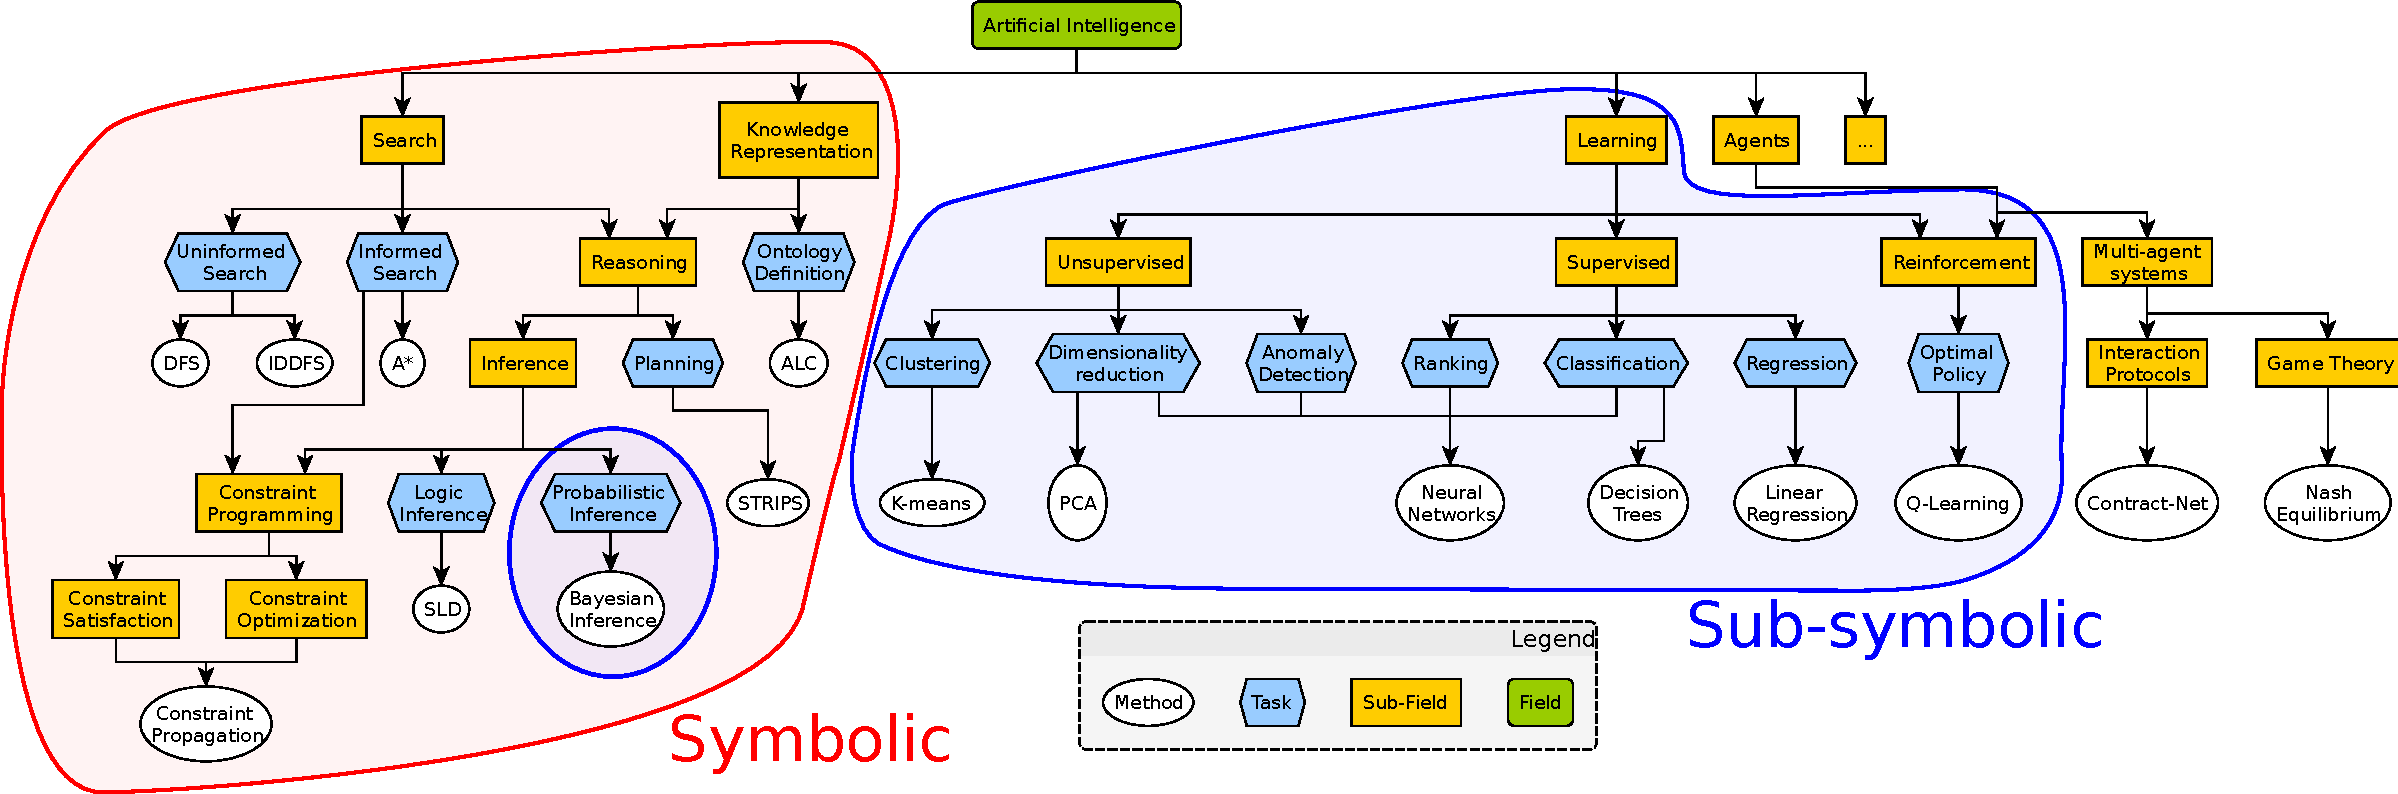
\includegraphics[angle=90, height=0.9\textheight]{figures/ai-map2}
    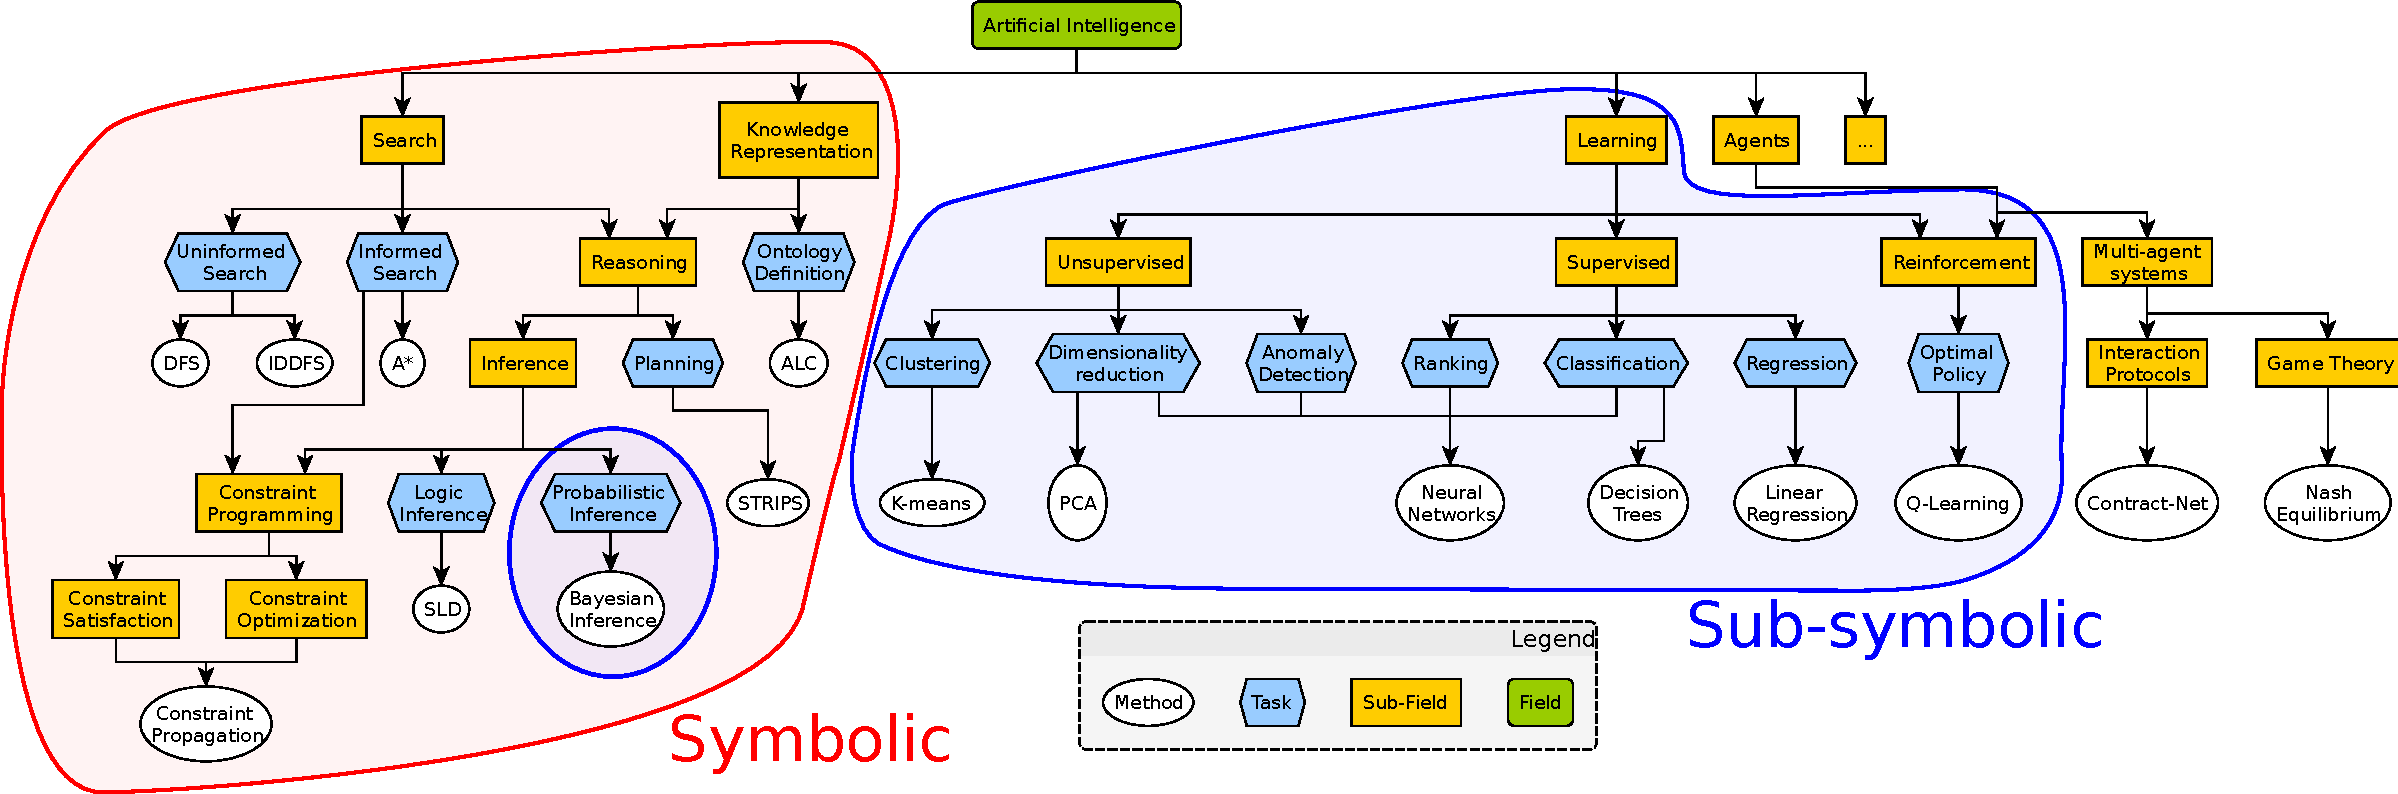
\includegraphics[width=\textwidth]{figures/ai-map2}
    \caption[Overview of the field of artificial intelligence]{
        \Gls{AI} map (not exhaustive) illustrating the main subfields with a focus on symbolic and sub-symbolic approaches.
        %
        On the left side, symbolic \gls{AI} is represented by search algorithms, \glspl{KR}, and reasoning.
        %
        On the right side, sub-symbolic \gls{AI} is represented by learning technique families, such as unsupervised learning, supervised learning, and reinforcement learning.
    }
    \label{fig:ai-map}
\end{figure}


\paragraph{Local vs. distributed}
%
Multidimensional arrays are the fundamental building block of sub-symbolic data representation.
%
Formally, a $D$-order array is an ordered container of real numbers, where $D$ indicates the number of indices required to access each element.
%
We refer to 1-order arrays as \emph{vectors}, 2-order arrays as \emph{matrices}, and arrays of order greater than two as \emph{tensors}.
%
In sub-symbolic tasks based on arrays, information is typically conveyed both by the values stored in the array and their position within it.
%
The dimensions of the array -- denoted as $(d_1 \times \dots \times d_D)$ -- also play a crucial role, as sub-symbolic systems are usually designed to operate on arrays of fixed shape.
%
That is, the values of $d_1, \dots, d_D$ are chosen at design time and remain unchanged thereafter.
%
This violates \Cref{itm:symbolic-req-2} above; accordingly, we define sub-symbolic \gls{KR} as the task of encoding information into rigid numeric arrays.
%
\emph{Local} and \emph{distributed} representations are two key modes for encoding data into such arrays.
%
In local representations, each entry in the array corresponds to a well-defined concept from the target domain---its semantic meaning is clear and independent.
%
In distributed representations, by contrast, individual values carry little or no standalone meaning: their interpretation depends on the configuration of values across a neighbourhood in the indexing space.
%
Consequently, while the exact location of values is largely irrelevant in local representations, it becomes essential in distributed ones.
%
Notably, distributed representations violate \Cref{itm:symbolic-req-3}, and for this reason, recent literature often labels as \emph{sub-symbolic} those predictors that rely on distributed encoding of data.

%----------------------------------------------------------------------------------------
%------------------------------------ Symbolic AI ---------------------------------------
%----------------------------------------------------------------------------------------

\subsection[Symbolic AI]{Symbolic \Gls{AI}}\label{subsec:symbolic-ai}
%
Symbolic \gls{AI} has been regarded as crucial since \gls{AI}'s inception.
%
Symbolic \gls{KR} offers enhanced flexibility, expressiveness, and intelligibility, being interpretable both by machines and by humans.

\paragraph{Intentional vs. extensional}
%
In formal logic, one may define concepts either \emph{extensionally} or \emph{intensionally}.
%
Extensional definitions are direct representations of data.
%
For example, the set of square numbers admits the extensional definition $\{0,1,4,9,16,\dots\}$ by listing every member explicitly.
%
Conversely, an \emph{intensional} definition is an indirect representation of data.
%
In \gls{FOL}, this corresponds to defining a relation via a formula; for instance, the set of square numbers can be defined as $\{\,x\mid \exists n\in\mathbb{Z}\,(x = n^2)\}$ which succinctly encodes an infinite extension with a single schema.
%
Recursive intensional predicates further enhance expressivity: for example, the ancestor relation can be axiomatized by $\mathit{Ancestor}(x,y)\;\Leftrightarrow\;\mathit{Parent}(x,y)\;\lor\;\exists z\,[\,\mathit{Parent}(x,z)\wedge\mathit{Ancestor}(z,y)\,]$ allowing a compact representation of an infinite set of pairs with a finite rule.
%
In formal logic, intensional definitions are prized for their ability to model potentially unbounded domains within finite logical formalisms.


\paragraph{Expressiveness vs. tractability}
%
\begin{SCfigure}
    \centering
    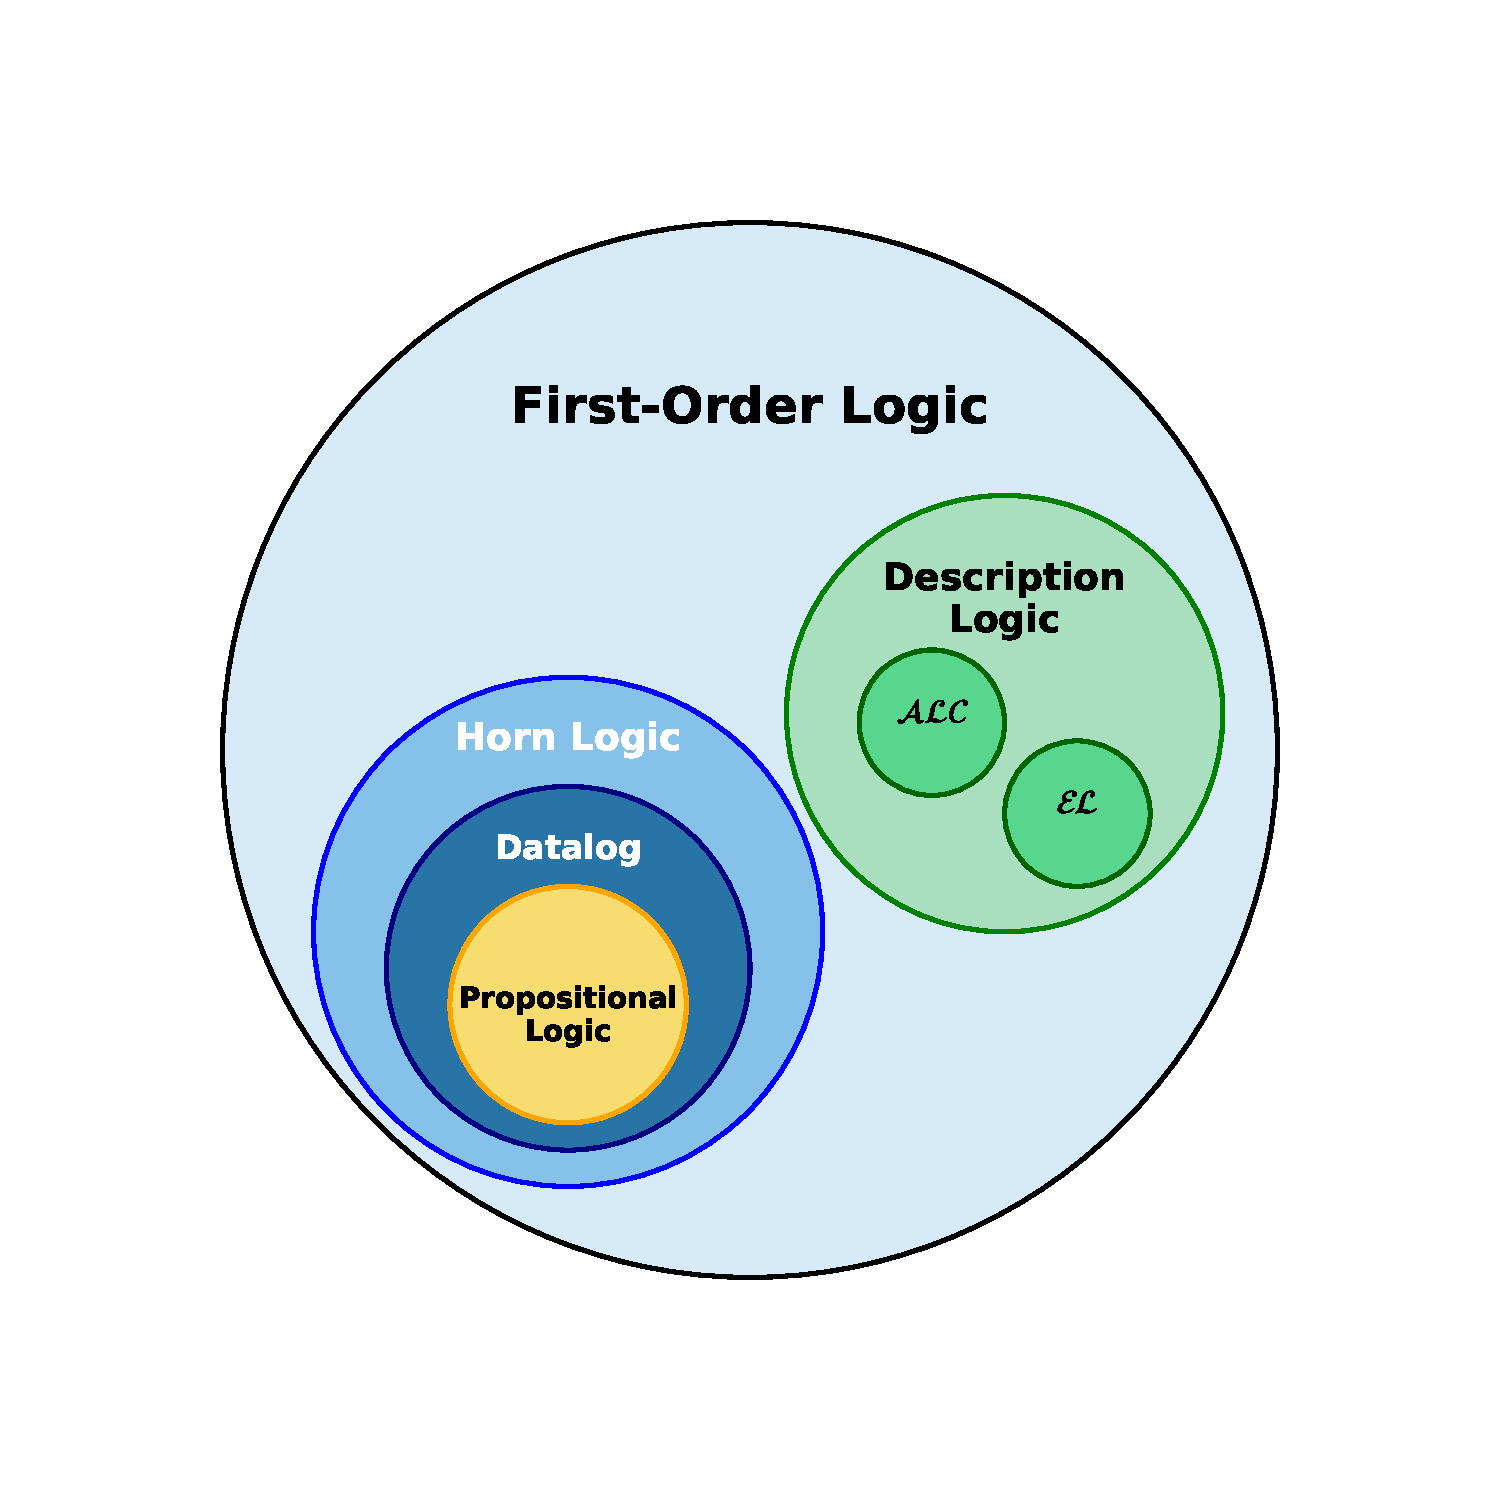
\includegraphics[width=0.58\textwidth]{figures/venn_diagram_logics}
    \caption[Venn diagram of different logic families]{
        %
        Venn diagram of different logic families, illustrating the trade-off between expressiveness and tractability.
        %
        \Gls{FOL} is the most expressive logic -- not the most expressive logic in general -- encompassing all others.
        %
        On the other hand, propositional logic is the least expressive, as it can only represent atomic propositions and their combinations.
        %
        All the other logics fall somewhere in between, with varying degrees of expressiveness and tractability.
    }
    \label{fig:venn-diagram-logics}
\end{SCfigure}

%
Tractability addresses the theoretical question of whether a logic reasoner can determine the truth of a given formula within feasible time and space bounds.
%
The answer is deeply tied to the specific reasoning algorithm and the logic's formal properties.
%
Depending on the features a logic provides -- such as quantifiers, function symbols, or recursive definitions -- it may be more or less expressive.
%
The higher the expressiveness, the more complex the problems that can be represented and reasoned about, but this also increases the computational burden.
%
This well-known phenomenon is often referred to as the expressiveness/tractability trade-off~\cite{DBLP:journals/jlp/CadoliS93,BRACHMAN2004327,DBLP:journals/ci/LevesqueB87}.
%
In practice, highly expressive logics make it easier for human users to model rich domains, often requiring fewer and more concise formulas.
%
However, this comes at the cost of automated inference, which may become computationally intractable, undecidable, or non-terminating in the general case.
%
To mitigate this issue, various fragments and extensions of \gls{FOL} have been identified, each providing different tradeoffs between what can be expressed and what can be decided efficiently.
%
\Cref{fig:venn-diagram-logics} illustrates the relationships among different logic families, highlighting the trade-off between expressiveness and tractability.


\subsubsection[First-order logic]{\Glsentrylong{FOL}}\label{subsubsec:first-order-logic}
%
\Gls{FOL} is a general-purpose formalism that underpins most symbolic \gls{KR} systems.
%
It enables both human and computational agents to model entities and their interrelations through predicates and terms within a defined domain of discourse.
%
Its syntax comprises variables (quantified explicitly or implicitly), constants, function symbols, and predicate symbols, which are combined via logical operators such as conjunction (\(\wedge\)), disjunction (\(\vee\)), implication (\(\rightarrow\)), and equivalence (\(\leftrightarrow\)).
%
\Gls{FOL} allows for both \emph{extensional} and \emph{intensional} definitions.
%
Recursive intensional definitions, in particular, are powerful, enabling finite representations of infinite sets.
%
Despite its flexibility, \gls{FOL} is semi-decidable in general: there is no algorithm that can determine the truth of every \gls{FOL} formula in finite time, which limits its use in systems requiring guaranteed termination~\cite{DBLP:conf/dlog/2003handbook}.


\subsubsection{Horn logic}\label{subsubsec:horn-logic}
%
Horn logic is a significant subset of \gls{FOL}, offering a balanced trade-off between theoretical expressiveness and practical tractability~\cite{DBLP:journals/jcss/Makowsky87}.
%
It is built around the concept of \emph{Horn clauses}~\cite{DBLP:journals/jsyml/Horn51}, which are formulas in \gls{FOL} that exclude quantifiers and consist of a disjunction of predicates, with at most one non-negated literal.
%
Alternatively, a Horn clause can be expressed as an implication where the consequent is a single predicate and the antecedent is a conjunction of predicates: \(h \gets b_1, \dots, b_n\).
%
Here, \(\gets\) denotes logical implication (from right to left), commas represent logical conjunctions, and \(b_i\) as well as \(h\) are predicates of arbitrary arity, potentially containing \gls{FOL} terms such as variables, constants, or functions.

Horn clauses can be interpreted as \emph{if-then} rules written in reverse order, where only conjunctions of predicates are allowed in the antecedent.
%
In essence, Horn logic is a constrained subset of \gls{FOL} characterized by the following limitations:
%
\begin{inlinelist}
%
    \item formulas are reduced to clauses, containing only predicates, conjunctions, and a single implication operator;
    %
    \item operators such as \(\lor\), \(\leftrightarrow\), or \(\neg\) (negation) are not allowed;
    %
    \item variables are implicitly quantified; and
    %
    \item terms behave as they do in \gls{FOL}.
    %
\end{inlinelist}


\subsubsection{Datalog}\label{subsubsec:datalog}
%
Datalog is a declarative query language and a restricted subset of \gls{FOL}, designed for deductive databases and knowledge representation~\cite{DBLP:journals/jcss/AjtaiG94}.
%
It represents knowledge using function-free Horn clauses, as defined in \Cref{subsubsec:horn-logic}.
%
This restriction eliminates the use of function symbols, thereby forbidding structured terms such as recursive data structures.
%
As a result, Datalog is well-suited for applications requiring finite and decidable reasoning, as the absence of function symbols ensures termination of inference algorithms.
%
Similar to Horn logic, Datalog’s knowledge bases consist of sets of function-free Horn clauses, which are interpreted as rules and facts.
%
Rules in Datalog follow the form \(h \gets b_1, \dots, b_n\), where \(h\) is the head of the rule and \(b_1, \dots, b_n\) are the body predicates.
%
Unlike general \gls{FOL}, Datalog does not allow disjunctions, negations, or explicit quantifiers, as variables are implicitly universally quantified.
%
Datalog is widely used in areas such as \glspl{KG}, semantic web technologies, and database systems, where efficient reasoning over large datasets is required.
%
Its simplicity and computational efficiency make it a practical choice for symbolic \gls{AI} tasks that demand tractable reasoning.


\subsubsection[Description logic]{\Glsentrylong{DL}}\label{subsubsec:dl}
%
\Gls{DL} are a family of subsets of \gls{FOL}, typically involving limited or no quantifiers, no structured terms, and no \textit{n}-ary predicates where \(n \geq 3\)~\cite{DBLP:books/daglib/0041477}.
%
In essence, \gls{DL} represents knowledge using constants and variables, along with atomic, unary, and binary predicates.


The differences among specific variants of \gls{DL} lie in the set of supported logical connectives and whether negation is allowed.
%
The wide variety of \gls{DL} stems from the well-known trade-off between expressiveness and tractability.
%
Depending on the application, one may prefer a more expressive \gls{DL} variant, which offers richer features at the cost of reduced tractability or even decidability of algorithms manipulating the knowledge, or vice versa.


In \gls{DL}, it is common practice to use specific terminology for different elements of knowledge representation:
%
\begin{itemize}
    %
    \item Constant terms are referred to as \textit{individuals}, as each constant represents a single entity within a domain.
    %
    \item Unary predicates are called \textit{classes} or \textit{concepts}, grouping sets of individuals for which the predicate holds true.
    %
    \item Binary predicates are referred to as \textit{properties} or \textit{roles}, connecting pairs of individuals.
    %
\end{itemize}
%

Using this nomenclature, knowledge in \gls{DL} can be represented by associating entities with constants (e.g., URLs) and defining concepts and properties accordingly.
%
Binary predicates are particularly significant as they enable the connection of pairs of entities.
%
This is typically achieved through subject–predicate–object triplets, represented as ground binary predicates of the form \(\langle a \, f \, b\rangle\) or \(f(a, b)\), where \(a\) is the subject, \(f\) is the predicate, and \(b\) is the object.

Collections of such triplets form \glspl{KG}, which are directed graphs where vertices represent individuals and arcs represent binary properties connecting these individuals.
%
\glspl{KG} may explicitly or implicitly instantiate a specific ontology, which is a formal description of classes characterizing a domain, their relationships (e.g., inclusion, exclusion, intersection, equivalence), and the properties they must or must not include.


\glspl{DL} are widely used in applications such as semantic web~\cite{DBLP:conf/coopis/GangemiM03} and ontology engineering~\cite{DBLP:books/ios/HGJKP2016}, where efficient reasoning and knowledge representation are essential.
%
Their ability to balance expressiveness and computational efficiency makes them a cornerstone of symbolic reasoning systems.


\subsubsection[Ontologies and knowledge graph]{Ontologies and \glsentrylong{KG}}\label{subsubsec:ontologies-and-kg}
%
An ontology is a formal and explicit specification of a shared conceptualisation of a domain~\cite{DBLP:books/daglib/p/Grimm10}.
%
It provides a structured vocabulary to describe the entities relevant in that domain, along with their attributes and the relationships among them.
%
This organisation enables both human understanding and machine-based reasoning.

Ontologies are typically expressed using \glspl{DL}, a family of logic-based formalisms for knowledge representation.
%
\Glspl{DL} define three main components:
%
\begin{inlinelist}
    %
    \item\emph{concepts} (or \emph{classes}), which group entities sharing similar features;
    %
    \item\emph{individuals} (or \emph{instances}), which are the concrete elements of the domain;
    %
    \item\emph{roles} (or \emph{properties}), which describe binary relationships between individuals.
    %
\end{inlinelist}
%
Different \glspl{DL} vary in their expressive power: for example, \gls{EL} supports only conjunction and existential quantification to ensure efficient reasoning, while more expressive DLs like \gls{ALC} allow for full Boolean operators and universal quantification.

Concepts are typically denoted using capital italic letters, such as $\mathit{Animal}$ or $\mathit{Cat}$.
%
These can be combined using logical constructors like intersection ($\sqcap$), union ($\sqcup$), or negation ($\lnot$) to form more complex classes.
%
A statement like $\mathit{Cat} \sqsubseteq \mathit{Animal}$ expresses that all cats are animals.

Individuals are constants representing specific entities in the domain and are usually written in monospaced lowercase, for example \texttt{tom}.
%
Membership of an individual in a concept is denoted using the ``is-a'' relation, written as \texttt{tom}~:~$\mathit{Cat}$, meaning ``Tom is a cat.''
%
Each individual may belong to multiple concepts.

Roles represent binary relations between individuals and are written in lowercase sans-serif font, such as \textsf{eats}.
%
They connect pairs of individuals, and their domain and range can be restricted using expressions such as $\textsf{eats} \sqsubseteq \mathit{Animal} \times \mathit{Edible}$.
%
Assertions like $\textsf{eats}(\texttt{tom}, \texttt{mouse})$ state that Tom eats the mouse.

The subsumption relation ($\sqsubseteq$) is used to express inclusion between concepts or roles.
%
For instance, $\mathit{Cat} \sqsubseteq \mathit{Animal}$ means that every cat is also an animal, and $\textsf{predatorOf} \sqsubseteq \textsf{eats}$ means that every predator-prey relationship implies eating.
%
Special concepts such as $\top$ and $\bot$ are used to denote the most general and the most specific concepts, respectively.

Collections of such axioms form an ontology.
%
\Gls{TBOX} define concepts and roles and their interrelations, while \gls{ABOX} specify which individuals belong to which concepts or are related via which roles.

\Glspl{KG} also provide a structured way to represent knowledge as graphs.
%
They consist of triplets (or \emph{facts}) of the form $(s, p, o)$, where $s$ is the subject, $p$ is the predicate (or property), and $o$ is the object.
%
These triplets form a directed graph where nodes represent individuals and edges represent relationships.

Unlike ontologies, KGs do not necessarily impose formal constraints on the structure or semantics of the triplets.
%
This flexibility allows for representing heterogeneous and incomplete data.
%
However, some \glspl{KG} are explicitly grounded in an ontology, and may follow its vocabulary and logical constraints.

In summary, ontologies and knowledge graphs both aim to formally capture structured knowledge.
%
Ontologies provide formal semantics and enable logical reasoning, while knowledge graphs emphasise scalability and flexibility in representing factual data.


\subsubsection{Propositional Logic}\label{subsubsec:propositional-logic}
%
Propositional logic is a restricted subset of \gls{FOL} in which quantifiers, terms, and non-atomic predicates are absent.
%
Its language consists solely of atomic propositions—also called 0-ary predicates—combined using standard logical connectives such as conjunction ($\land$), disjunction ($\lor$), negation ($\lnot$), and implication ($\rightarrow$).
%
Each proposition can be interpreted as a Boolean variable that takes a truth value in \{\texttt{true}, \texttt{false}\}.
%
The semantics of propositional logic aligns with Boolean algebra, making it straightforward to evaluate the truth of a formula given the truth values of its atomic components.

For example, a propositional formula such as $p \land \lnot q \rightarrow r$ can be interpreted as follows:
%
$p$ might stand for the proposition ``it is raining,'' $q$ for ``there is a roof,'' and $r$ for ``the floor is wet.''
%
In this case, the formula asserts that if it is raining and there is no roof, then the floor will be wet.

Compared to \gls{FOL}, propositional logic is significantly less expressive.
%
The absence of quantifiers means that general statements over a domain cannot be made.
%
Similarly, the lack of terms prevents direct reference to entities in the domain.
%
As a consequence, each relevant aspect of a scenario must be explicitly encoded as an individual proposition.

This limitation in expressiveness has important computational implications.
%
In particular, determining the satisfiability of a propositional formula is a decidable problem.
%
This makes propositional logic attractive in scenarios where tractable reasoning is required.

Despite its apparent simplicity, propositional logic can model a surprising range of situations.
%
Expressions involving numerical constants, variables, and comparisons (e.g., $x > 5$ or $y = 3$) can be encoded propositionally by introducing a distinct Boolean variable for each comparison.
%
This reduction allows the use of propositional logic in settings where the original problem does not explicitly involve logical variables or quantifiers, but can be decomposed into atomic truth conditions.


\subsubsection[Limits of symbolic AI]{Limits of symbolic \Gls{AI}}\label{subsubsec:limits-of-symbolic-ai}


%-----------------------------------------------------------------------------------------
%------------------------------------ Sub-symbolic AI ------------------------------------
%-----------------------------------------------------------------------------------------

\subsection[Sub-symbolic AI]{Sub-symbolic \Gls{AI}}\label{subsec:sub-symbolic-ai}
%
Sub-symbolic \gls{AI} encompasses a wide range of techniques that rely on numerical representations.
%
Contributions come from varius fields, including \gls{ML}, statistical learning, and data mining.
%
The huge number of approaches is also motivated by the well known \gls{NFL} theorem~\cite{DBLP:journals/tec/DolpertM97} that states that no single learning algorithm can outperform all others across all possible tasks.
%
The most common predictor families are linear models, \glspl{DT}, \glspl{RF}, \glspl{SVM}, \glspl{NN} (including \glspl{LLM}), and many others.


\paragraph{Predictive performance vs. interpretability}
%
\begin{figure}[h]
    \centering
    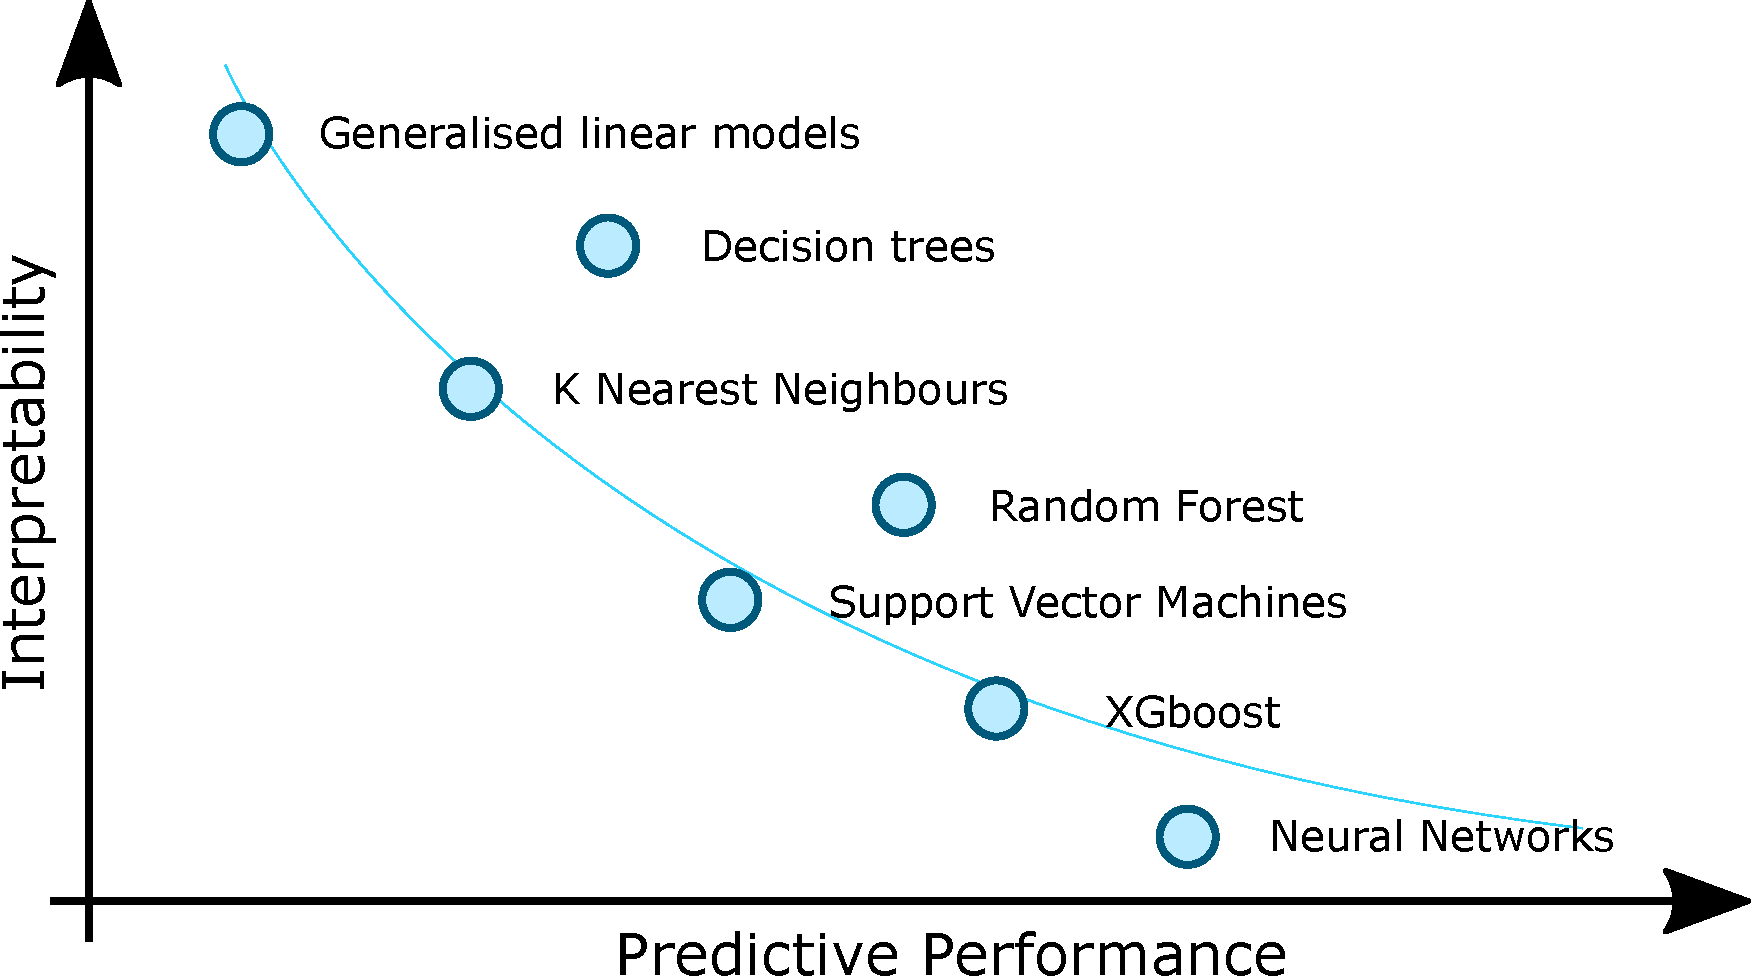
\includegraphics[width=0.9\textwidth]{figures/interpretability-performance-tradeoff}
    \caption[Performance vs. interpretability trade-off]{
        %
        Trade-off between predictive performance and interpretability in common sub-symbolic predictors.
        %
        The figure illustrates how different predictor families balance these two aspects, with simpler models being more interpretable but potentially less accurate.
        %
    }
    \label{fig:performance-vs-interpretability}
\end{figure}
%
The \emph{complexity} of a sub-symbolic predictor can vary significantly.
%
By complexity we mean the overall structure of the model, including the number of parameters, the operations that are performed, and possibly the way the model is trained.
%
\Glspl{DT}, for example, are relatively simple models that can be easily interpreted by humans.
%
The downside of \glspl{DT} is that they make predictions by linearly partitioning the input space, which can lead to poor generalisation on unseen data.
%
On the other hand, \glspl{NN} can be extremely complex, with millions of parameters and intricate architectures that are difficult to interpret.
%
However, \glspl{NN} can capture highly non-linear relationships in the data, often leading to superior predictive performance compared to simpler models.
%
The definition of interpretability is not univocal, and it lacks measures that are widely accepted~\cite{DBLP:journals/natmi/Rudin19}.
%
Despite that, \Cref{fig:performance-vs-interpretability} illustrates in an informal way the trade-off between predictive performance and interpretability in sub-symbolic predictors.


\subsubsection[Non-neural models]{\Glsentrylongpl{DT}}\label{subsubsec:non-neural-models}
%
\paragraph{Decision trees}
%
\Glspl{DT} are a family of predictors that support both classification and regression tasks.
%
During the learning phase, the input space is recursively partitioned into multiple regions through a series of splits (i.e., decisions) based on the input data \(X\).
%
Each region is associated with a constant prediction, and the splits are designed to minimize the error with respect to the expected outputs \(Y\), while keeping the total number of regions low.
%
The learning process synthesizes a hierarchical structure of decision rules, which are followed to compute predictions for any \(x \in X\).
%
In the inference phase, these decision rules are evaluated sequentially, starting from the root of the tree and proceeding to a leaf node.
%
Each leaf corresponds to a specific region of the input space, resulting in a single prediction for each \(x\).

Unlike other predictor families, \glspl{DT} produce a tree of decision rules as the outcome of the learning process.
%
This tree is straightforwardly interpretable by humans and can be graphically represented in two-dimensional charts.
%
This property is particularly valuable when the internal workings of an automatic predictor need to be understood by a human agent.
%
\Glspl{DT} are often used in applications where interpretability is crucial, as their structure provides clear insights into the decision-making process.
%
For further details on the advantages and limitations of \glspl{DT}, refer to \Cref{subsubsec:limits-of-sub-symbolic-ai}.


\paragraph[Random forests]{\Glsentrylongpl{RF}}


\paragraph[Support vector machines]{\Glsentrylongpl{SVM}}


\subsubsection[Neural networks]{\Glsentrylongpl{NN}}\label{subsubsec:neural-networks}
\note{Todo: add figures representing the architectures and how it works.}
%
\Glspl{NN} are a family of predictors inspired by the structure and function of biological neural networks.
%
They consist of interconnected nodes (neurons) interconnected into a \gls{DAG} and organized into layers, where each neuron receives inputs, applies a non-linear activation function, and produces an output.
%
Despite being very popular nowadays, the first idea of a \gls{NN} has been proposed back in 1943~\cite{mcculloch1943logical}.
%
The so-called perceptron -- a single-layer \gls{NN} -- has been introduced in 1958~\cite{rosenblatt1958perceptron}.
%
Due to the limited expressiveness of single-layer \glspl{NN}, the perceptron could only learn linearly separable functions~\cite{DBLP:books/daglib/0066902}.

To overcome these limitations, researchers proposed to stack multiple layers of neurons, leading to the concept of \glspl{MLP}.
%
Although the theoretical foundations of such models were clear early on, the lack of an effective training algorithm hindered their practical use.
%
This changed with the rediscovery and popularization of the \textit{backpropagation} algorithm in the 1980s~\cite{rumelhart1986learning}, which allowed efficient computation of gradients through multiple layers using the chain rule of calculus.
%
This innovation enabled \glspl{MLP} to learn complex non-linear functions and marked the beginning of modern \gls{NN} research.

Many different architectures have been proposed since then, including fully connected \glspl{NN}, \glspl{CNN}, \glspl{RNN}, and more.
%
These architectures are designed specifically to handle different types of data and tasks, such as image classification, natural language processing, and time series analysis.

\paragraph{Feedforward Neural Networks.}
%
The simplest class of \glspl{NN} is the family of feedforward networks, in which information flows unidirectional from the input layer through one or more hidden layers to the output layer, without forming cycles.
%
Among these, \glspl{MLP} are the canonical example, consisting of fully connected layers interleaved with non-linear activation functions.
%
Given sufficient capacity, \glspl{MLP} are universal function approximators~\cite{hornik1989multilayer}, capable of representing any Borel measurable function under mild assumptions.
%
Despite their theoretical expressiveness, \glspl{MLP} are inefficient when processing structured inputs such as images or sequences, as they fail to exploit the inherent inductive biases of the data.

\paragraph{Convolutional Neural Networks.}
%
To overcome the limitations of \glspl{MLP} on grid-like data such as images, \glspl{CNN} were introduced.
%
Pioneering work on hierarchical feature extraction was done by Fukushima with the Neocognitron~\cite{fukushima1980neocognitron}, followed by the successful application of convolutional networks to handwritten digit classification in LeNet-5~\cite{lecun1998gradient}.
%
\glspl{CNN} apply learnable convolutional filters that exploit local spatial correlations, reducing the number of parameters and enabling translation equivariance.
%
Pooling layers further promote translation invariance by down sampling intermediate representations.
%
These properties make \glspl{CNN} particularly well-suited for tasks involving visual perception.

\paragraph{Recurrent Neural Networks.}
%
In contrast, \glspl{RNN} are designed for processing sequential data by incorporating temporal recurrence.
%
Each unit in an \gls{RNN} receives input not only from the current time step but also from its own past activations, effectively providing a form of memory across time.
%
This architecture allows \glspl{RNN} to model temporal dependencies and variable-length input sequences.
%
However, standard \glspl{RNN} suffer from the vanishing and exploding gradient problems~\cite{bengio1994learning}, which hinder their ability to learn long-range dependencies.
%
To address these issues, more sophisticated variants were developed, notably \glspl{LSTM} (Long Short-Term Memory)~\cite{hochreiter1997long} and \glspl{GRU} (Gated Recurrent Units)~\cite{cho2014learning}, which introduce gating mechanisms to regulate information flow and preserve long-term context.


\subsubsection[Limits of sub-symbolic AI]{Limits of sub-symbolic \Gls{AI}}\label{subsubsec:limits-of-sub-symbolic-ai}


%-----------------------------------------------------------------------------------------
%----------------------------------- AI and society --------------------------------------
%-----------------------------------------------------------------------------------------

\section{AI and society}\label{sec:ai-and-society}
%
\subsection[Explainable AI]{\Glsentrylong{XAI}}\label{subsec:xai}
%
Modern intelligent systems increasingly rely on sub-symbolic predictive models to support their intelligent behaviour.
%
These models are typically trained using a data-driven approach, leveraging the vast availability of data generated in recent years.
%
\Gls{ML} algorithms enable the semi-automatic detection of statistical patterns hidden within data.
%
Such patterns can then be used to support decision-making, planning, and forecasting across various domains where data is available.


Despite their predictive capabilities, \gls{ML} models face significant challenges in critical applications.
%
One of the most notable issues is \emph{algorithmic opacity}, which refers to the difficulty humans face in understanding how these models operate or make decisions.
%
Opacity arises due to the complex interplay between high-dimensional datasets, the algorithms processing them, and the dynamic behaviour of these algorithms during training~\cite{DBLP:journals/bigdatasociety/Burrell16}.
%
This lack of transparency is particularly problematic in domains such as healthcare, finance, and law, where human accountability and explainability are essential.


The term \emph{black box} is often used to describe \gls{ML} predictors, as their internal workings are not symbolically represented~\cite{interpretability-lipton-2018}.
%
Without symbolic representations, it becomes challenging for humans to comprehend the operation of these systems or the rationale behind their decisions.
%
This can lead to a lack of trust and acceptance of \gls{AI}-based solutions.


Regulatory frameworks, such as the \gls{GDPR}, have started to recognise the \emph{right to explanation}~\cite{DBLP:journals/aim/GoodmanF17}.
%
This right mandates that intelligent systems must be understandable to ensure fairness, identify biases, and verify that they function as intended.
%
However, the concept of \emph{understandability} remains neither standardised nor systematically assessed~\cite{DBLP:journals/ai/Miller19}.
%
While some \gls{ML} models are more interpretable than others, there is no consensus on what constitutes an adequate explanation.


Interpretability and explainability are desirable properties for intelligent systems.
%
\Gls{XAI} aims to make sub-symbolic \gls{AI} more interpretable for humans, often by automating the generation of explanations.
%
Interpretability refers to the cognitive effort required by humans to assign meaning to the behaviour or outcomes of intelligent systems.
%
It is often associated with properties such as algorithmic transparency, decomposability, and predictability.


An \emph{explanation}, on the other hand, is a set of statements or accounts that clarify an object or justify an action.
%
Explanations can involve constructing more interpretable representations of a black-box model.
%
For instance, \emph{model simplification} techniques translate a complex model into a simpler one with high fidelity~\cite{DBLP:conf/kdd/TolomeiSHL17,DBLP:journals/csur/GuidottiMRTGP19}.
%
Alternatively, symbolic knowledge can be extracted from sub-symbolic predictors, producing interpretable objects from less interpretable ones.


Another approach to improving interpretability involves injecting symbolic knowledge into sub-symbolic predictors.
%
This process does not produce explanations but increases the model's transparency by aligning its behaviour with more interpretable systems.

Interpretability and explainability enhance trustworthiness in \gls{AI}-based solutions.
%
However, they also enable users to exercise finer control over these systems, deciding whether to trust them or not~\cite{10.1214/21-SS133}.
%
The surveyed \gls{SKE} and \gls{SKI} methods should be regarded as tools for increasing user control over \gls{AI} systems.


\subsection{Sorts of Explanation}\label{subsec:sorts-of-explanation}
%
Two major approaches exist to bring explainability or interpretability to intelligent systems: \emph{by design} and \emph{post-hoc}~\cite{DBLP:conf/atal/CiattoSOC20,DBLP:journals/inffus/ArrietaRSBTBGGM20,DBLP:journals/csur/GuidottiMRTGP19}.


\paragraph{\Gls{XAI} by Design}
\label{par:xai-by-design}
%
This approach aims to make systems interpretable or explainable from the outset, treating these features as primary design goals.
%
Methods in this category can be further divided into:
%
\begin{itemize}
    \item \emph{Symbols as constraints}, where predictive models are constrained by symbolic rules, often expressed in subsets of \gls{FOL}.
    \item \emph{Transparent box design}, where models are inherently interpretable and require no further manipulation.
\end{itemize}

\paragraph{Post-hoc Explainability}
%
This approach involves manipulating pre-existing systems to make them interpretable or explainable.
%
Methods in this category include:
%
\begin{itemize}
    \item \emph{Text explanation}, which generates textual descriptions of model behaviour.
    \item \emph{Visual explanation}, which visualises model behaviour, often using dimensionality reduction techniques.
    \item \emph{Local explanation}, which segments the solution space into simpler subspaces and explains them.
    \item \emph{Explanation by example}, which extracts representative examples to illustrate internal relationships.
    \item \emph{Model simplification}, which constructs a simplified system that optimises similarity to the original while reducing complexity.
    \item \emph{Feature relevance}, which assigns relevance scores to features, revealing their importance in the model's output.
\end{itemize}


\subsection[Fairness in AI]{Fairness in \gls{AI}}
\label{subsec:fairness-in-ai}

\note{TODO: introduction to fairness in AI, why it is important, and how it relates to this work.}


\subsection{Data protection and privacy}
\label{subsec:data-protection-and-privacy}

\note{TODO: introduction to data protection and privacy, why it is important, and how it relates to this work.}

%%! Author = matteomagnini
%! Date = 05/03/25

%----------------------------------------------------------------------------------------
\chapter[Artificial Intelligence]{\Glsentrylong{AI}}
\label{ch:ai}
\minitoc
%----------------------------------------------------------------------------------------

\section{Overview}\label{sec:ai-overview}
%
The wide range of \gls{AI} techniques used to be divided into two main categories: \emph{symbolic} and \emph{sub-symbolic} \gls{AI}.
%
The thing that distinguishes the two categories is the way they \emph{represent knowledge} and how they process it.
%
No intelligence can exist without knowledge and no computation can occur in lack of representation.
%
In the rest of the thesis, we will use the term symbolic (resp., sub-symbolic) \gls{AI} and symbolic (resp., sub-symbolic) \gls{KR} almost interchangeably.
%
Symbolic \gls{AI} is based on \emph{symbols}, which come with a \emph{meaning} and could be manipulated according to the formalism and rules of a given \gls{AI} system.
%
On the other hand, sub-symbolic \gls{AI} is based on a numerical representation -- a.k.a., sub-symbolic -- where the numbers are not directly interpretable.
%
Numbers are technically symbols, but numbers, arrays and their functions are not recognised as means for symbolic \gls{KR}.
%
According to Van Gelder~\cite{DBLP:conf/ogai/Gelder90}, in order to be considered symbolic, \gls{KR} approaches must:
%
\begin{requirements}
    %
    \item \label{itm:symbolic-req-1} involve a set of symbols;
    %
    \item \label{itm:symbolic-req-2} the symbols can be combined following a set of grammatical rules;
    %
    \item \label{itm:symbolic-req-3} elementary symbols and combinations of symbols can be assigned a meaning.
    %
\end{requirements}


\paragraph{Local vs. distributed}
%
Multidimensional arrays are the fundamental building block of sub-symbolic data representation.
%
Formally, a $D$-order array is an ordered container of real numbers, where $D$ indicates the number of indices required to access each element.
%
We refer to 1-order arrays as \emph{vectors}, 2-order arrays as \emph{matrices}, and arrays of order greater than two as \emph{tensors}.
%
In sub-symbolic tasks based on arrays, information is typically conveyed both by the values stored in the array and their position within it.
%
The dimensions of the array -- denoted as $(d_1 \times \dots \times d_D)$ -- also play a crucial role, as sub-symbolic systems are usually designed to operate on arrays of fixed shape.
%
That is, the values of $d_1, \dots, d_D$ are chosen at design time and remain unchanged thereafter.
%
This violates \Cref{itm:symbolic-req-2} above; accordingly, we define sub-symbolic \gls{KR} as the task of encoding information into rigid numeric arrays.
%
\emph{Local} and \emph{distributed} representations are two key modes for encoding data into such arrays.
%
In local representations, each entry in the array corresponds to a well-defined concept from the target domain---its semantic meaning is clear and independent.
%
In distributed representations, by contrast, individual values carry little or no standalone meaning: their interpretation depends on the configuration of values across a neighbourhood in the indexing space.
%
Consequently, while the exact location of values is largely irrelevant in local representations, it becomes essential in distributed ones.
%
Notably, distributed representations violate \Cref{itm:symbolic-req-3}, and for this reason, recent literature often labels as \emph{sub-symbolic} those predictors that rely on distributed encoding of data.


\section{Symbolic \Gls{AI}}\label{sec:symbolic-ai}
%
Symbolic \gls{AI} has been regarded as crucial since \gls{AI}'s inception.
%
Symbolic \gls{KR} offers enhanced flexibility, expressiveness, and intelligibility, being interpretable both by machines and by humans.

\paragraph{Intentional vs. extensional}
%
In formal logic, one may define concepts either \emph{extensionally} or \emph{intensionally}.
%
Extensional definitions are direct representations of data.
%
For example, the set of square numbers admits the extensional definition $\{0,1,4,9,16,\dots\}$ by listing every member explicitly.
%
Conversely, an \emph{intensional} definition is an indirect representation of data.
%
In \gls{FOL}, this corresponds to defining a relation via a formula; for instance, the set of square numbers can be defined as $\{\,x\mid \exists n\in\mathbb{Z}\,(x = n^2)\}$ which succinctly encodes an infinite extension with a single schema.
%
Recursive intensional predicates further enhance expressivity: for example, the ancestor relation can be axiomatized by $\mathit{Ancestor}(x,y)\;\Leftrightarrow\;\mathit{Parent}(x,y)\;\lor\;\exists z\,[\,\mathit{Parent}(x,z)\wedge\mathit{Ancestor}(z,y)\,]$ allowing a compact representation of an infinite set of pairs with a finite rule.
%
In formal logic, intensional definitions are prized for their ability to model potentially unbounded domains within finite logical formalisms.


\paragraph{Expressiveness vs. tractability}
%
\begin{SCfigure}
    \centering
    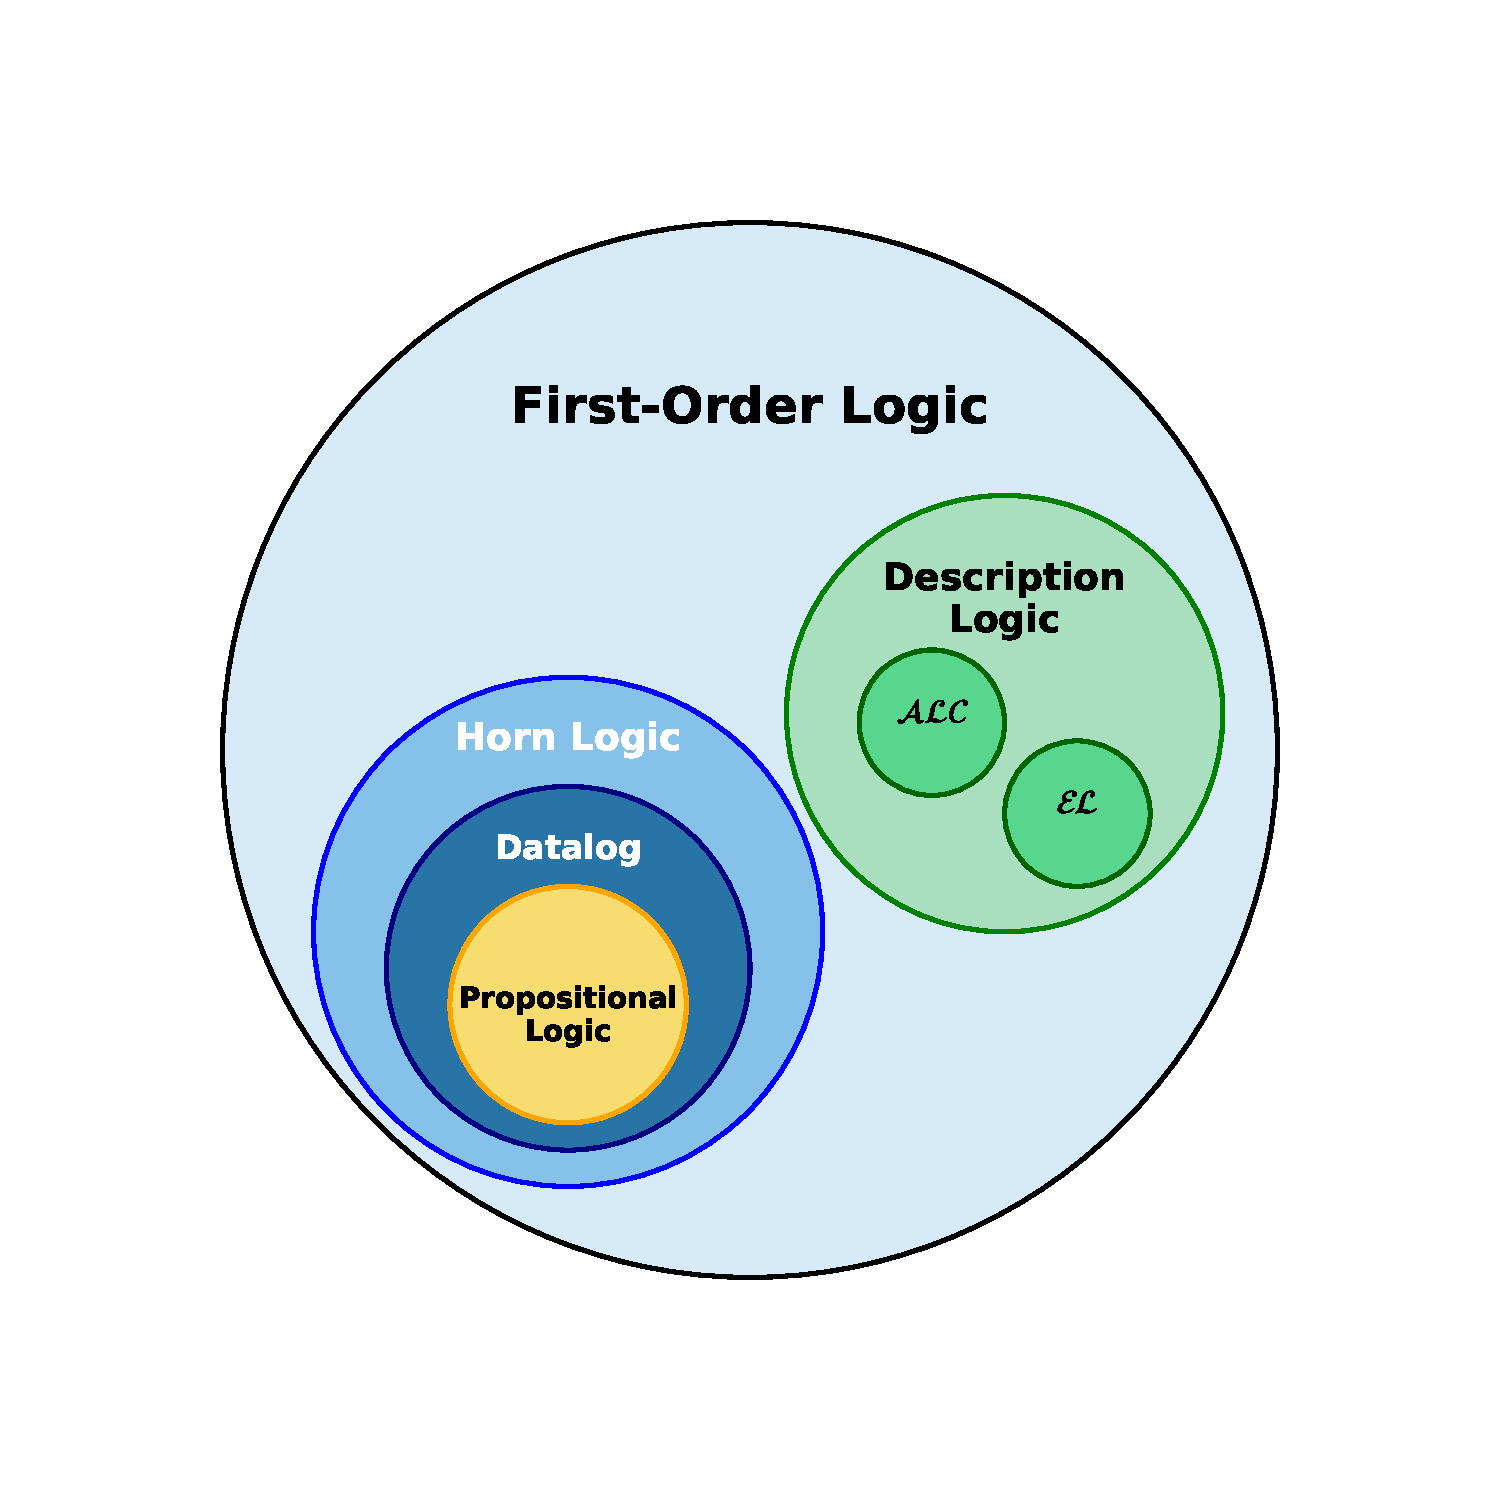
\includegraphics[width=0.58\textwidth]{figures/venn_diagram_logics}
    \caption[Venn diagram of different logic families]{
        %
        Venn diagram of different logic families, illustrating the trade-off between expressiveness and tractability.
        %
        \Gls{FOL} is the most expressive logic -- not the most expressive logic in general -- encompassing all others.
        %
        On the other hand, propositional logic is the least expressive, as it can only represent atomic propositions and their combinations.
        %
        All the other logics fall somewhere in between, with varying degrees of expressiveness and tractability.
    }
    \label{fig:venn-diagram-logics}
\end{SCfigure}

%
Tractability addresses the theoretical question of whether a logic reasoner can determine the truth of a given formula within feasible time and space bounds.
%
The answer is deeply tied to the specific reasoning algorithm and the logic's formal properties.
%
Depending on the features a logic provides -- such as quantifiers, function symbols, or recursive definitions -- it may be more or less expressive.
%
The higher the expressiveness, the more complex the problems that can be represented and reasoned about, but this also increases the computational burden.
%
This well-known phenomenon is often referred to as the expressiveness/tractability trade-off~\cite{DBLP:journals/jlp/CadoliS93,BRACHMAN2004327,DBLP:journals/ci/LevesqueB87}.
%
In practice, highly expressive logics make it easier for human users to model rich domains, often requiring fewer and more concise formulas.
%
However, this comes at the cost of automated inference, which may become computationally intractable, undecidable, or non-terminating in the general case.
%
To mitigate this issue, various fragments and extensions of \gls{FOL} have been identified, each providing different tradeoffs between what can be expressed and what can be decided efficiently.
%
\Cref{fig:venn-diagram-logics} illustrates the relationships among different logic families, highlighting the trade-off between expressiveness and tractability.


\subsection{\Glsentrylong{FOL}}\label{subsec:first-order-logic}
%
\Gls{FOL} is a general-purpose formalism that underpins most symbolic \gls{KR} systems.
%
It enables both human and computational agents to model entities and their interrelations through predicates and terms within a defined domain of discourse.
%
Its syntax comprises variables (quantified explicitly or implicitly), constants, function symbols, and predicate symbols, which are combined via logical operators such as conjunction (\(\wedge\)), disjunction (\(\vee\)), implication (\(\rightarrow\)), and equivalence (\(\leftrightarrow\)).
%
\Gls{FOL} allows for both \emph{extensional} and \emph{intensional} definitions.
%
Recursive intensional definitions, in particular, are powerful, enabling finite representations of infinite sets.
%
Despite its flexibility, \gls{FOL} is semi-decidable in general: there is no algorithm that can determine the truth of every \gls{FOL} formula in finite time, which limits its use in systems requiring guaranteed termination~\cite{DBLP:conf/dlog/2003handbook}.


\subsection{Horn logic}\label{subsec:horn-logic}
%
Horn logic is a significant subset of \gls{FOL}, offering a balanced trade-off between theoretical expressiveness and practical tractability~\cite{DBLP:journals/jcss/Makowsky87}.
%
It is built around the concept of \emph{Horn clauses}~\cite{DBLP:journals/jsyml/Horn51}, which are formulas in \gls{FOL} that exclude quantifiers and consist of a disjunction of predicates, with at most one non-negated literal.
%
Alternatively, a Horn clause can be expressed as an implication where the consequent is a single predicate and the antecedent is a conjunction of predicates: \(h \gets b_1, \dots, b_n\).
%
Here, \(\gets\) denotes logical implication (from right to left), commas represent logical conjunctions, and \(b_i\) as well as \(h\) are predicates of arbitrary arity, potentially containing \gls{FOL} terms such as variables, constants, or functions.

Horn clauses can be interpreted as \emph{if-then} rules written in reverse order, where only conjunctions of predicates are allowed in the antecedent.
%
In essence, Horn logic is a constrained subset of \gls{FOL} characterized by the following limitations:
%
\begin{inlinelist}
%
    \item formulas are reduced to clauses, containing only predicates, conjunctions, and a single implication operator;
    %
    \item operators such as \(\lor\), \(\leftrightarrow\), or \(\neg\) (negation) are not allowed;
    %
    \item variables are implicitly quantified; and
    %
    \item terms behave as they do in \gls{FOL}.
    %
\end{inlinelist}


\subsection{Datalog}\label{subsec:datalog}
%
Datalog is a declarative query language and a restricted subset of \gls{FOL}, designed for deductive databases and knowledge representation~\cite{DBLP:journals/jcss/AjtaiG94}.
%
It represents knowledge using function-free Horn clauses, as defined in \Cref{subsec:horn-logic}.
%
This restriction eliminates the use of function symbols, thereby forbidding structured terms such as recursive data structures.
%
As a result, Datalog is well-suited for applications requiring finite and decidable reasoning, as the absence of function symbols ensures termination of inference algorithms.
%
Similar to Horn logic, Datalog’s knowledge bases consist of sets of function-free Horn clauses, which are interpreted as rules and facts.
%
Rules in Datalog follow the form \(h \gets b_1, \dots, b_n\), where \(h\) is the head of the rule and \(b_1, \dots, b_n\) are the body predicates.
%
Unlike general \gls{FOL}, Datalog does not allow disjunctions, negations, or explicit quantifiers, as variables are implicitly universally quantified.
%
Datalog is widely used in areas such as \glspl{KG}, semantic web technologies, and database systems, where efficient reasoning over large datasets is required.
%
Its simplicity and computational efficiency make it a practical choice for symbolic \gls{AI} tasks that demand tractable reasoning.


\subsection{\Glsentrylong{DL}}\label{subsec:dl}
%
\Gls{DL} are a family of subsets of \gls{FOL}, typically involving limited or no quantifiers, no structured terms, and no \textit{n}-ary predicates where \(n \geq 3\)~\cite{DBLP:books/daglib/0041477}.
%
In essence, \gls{DL} represents knowledge using constants and variables, along with atomic, unary, and binary predicates.


The differences among specific variants of \gls{DL} lie in the set of supported logical connectives and whether negation is allowed.
%
The wide variety of \gls{DL} stems from the well-known trade-off between expressiveness and tractability.
%
Depending on the application, one may prefer a more expressive \gls{DL} variant, which offers richer features at the cost of reduced tractability or even decidability of algorithms manipulating the knowledge, or vice versa.


In \gls{DL}, it is common practice to use specific terminology for different elements of knowledge representation:
%
\begin{itemize}
    %
    \item Constant terms are referred to as \textit{individuals}, as each constant represents a single entity within a domain.
    %
    \item Unary predicates are called \textit{classes} or \textit{concepts}, grouping sets of individuals for which the predicate holds true.
    %
    \item Binary predicates are referred to as \textit{properties} or \textit{roles}, connecting pairs of individuals.
    %
\end{itemize}
%

Using this nomenclature, knowledge in \gls{DL} can be represented by associating entities with constants (e.g., URLs) and defining concepts and properties accordingly.
%
Binary predicates are particularly significant as they enable the connection of pairs of entities.
%
This is typically achieved through subject–predicate–object triplets, represented as ground binary predicates of the form \(\langle a \, f \, b\rangle\) or \(f(a, b)\), where \(a\) is the subject, \(f\) is the predicate, and \(b\) is the object.

Collections of such triplets form \glspl{KG}, which are directed graphs where vertices represent individuals and arcs represent binary properties connecting these individuals.
%
\glspl{KG} may explicitly or implicitly instantiate a specific ontology, which is a formal description of classes characterizing a domain, their relationships (e.g., inclusion, exclusion, intersection, equivalence), and the properties they must or must not include.


\glspl{DL} are widely used in applications such as semantic web~\cite{DBLP:conf/coopis/GangemiM03} and ontology engineering~\cite{DBLP:books/ios/HGJKP2016}, where efficient reasoning and knowledge representation are essential.
%
Their ability to balance expressiveness and computational efficiency makes them a cornerstone of symbolic reasoning systems.


\subsection{Ontologies and \glsentrylong{KG}}\label{subsec:ontologies-and-kg}
%
An ontology is a formal and explicit specification of a shared conceptualisation of a domain~\cite{DBLP:books/daglib/p/Grimm10}.
%
It provides a structured vocabulary to describe the entities relevant in that domain, along with their attributes and the relationships among them.
%
This organisation enables both human understanding and machine-based reasoning.

Ontologies are typically expressed using \glspl{DL}, a family of logic-based formalisms for knowledge representation.
%
\Glspl{DL} define three main components:
%
\begin{inlinelist}
    %
    \item\emph{concepts} (or \emph{classes}), which group entities sharing similar features;
    %
    \item\emph{individuals} (or \emph{instances}), which are the concrete elements of the domain;
    %
    \item\emph{roles} (or \emph{properties}), which describe binary relationships between individuals.
    %
\end{inlinelist}
%
Different \glspl{DL} vary in their expressive power: for example, \gls{EL} supports only conjunction and existential quantification to ensure efficient reasoning, while more expressive DLs like \gls{ALC} allow for full Boolean operators and universal quantification.

Concepts are typically denoted using capital italic letters, such as $\mathit{Animal}$ or $\mathit{Cat}$.
%
These can be combined using logical constructors like intersection ($\sqcap$), union ($\sqcup$), or negation ($\lnot$) to form more complex classes.
%
A statement like $\mathit{Cat} \sqsubseteq \mathit{Animal}$ expresses that all cats are animals.

Individuals are constants representing specific entities in the domain and are usually written in monospaced lowercase, for example \texttt{tom}.
%
Membership of an individual in a concept is denoted using the ``is-a'' relation, written as \texttt{tom}~:~$\mathit{Cat}$, meaning ``Tom is a cat.''
%
Each individual may belong to multiple concepts.

Roles represent binary relations between individuals and are written in lowercase sans-serif font, such as \textsf{eats}.
%
They connect pairs of individuals, and their domain and range can be restricted using expressions such as $\textsf{eats} \sqsubseteq \mathit{Animal} \times \mathit{Edible}$.
%
Assertions like $\textsf{eats}(\texttt{tom}, \texttt{mouse})$ state that Tom eats the mouse.

The subsumption relation ($\sqsubseteq$) is used to express inclusion between concepts or roles.
%
For instance, $\mathit{Cat} \sqsubseteq \mathit{Animal}$ means that every cat is also an animal, and $\textsf{predatorOf} \sqsubseteq \textsf{eats}$ means that every predator-prey relationship implies eating.
%
Special concepts such as $\top$ and $\bot$ are used to denote the most general and the most specific concepts, respectively.

Collections of such axioms form an ontology.
%
\Gls{TBOX} define concepts and roles and their interrelations, while \gls{ABOX} specify which individuals belong to which concepts or are related via which roles.

\Glspl{KG} also provide a structured way to represent knowledge as graphs.
%
They consist of triplets (or \emph{facts}) of the form $(s, p, o)$, where $s$ is the subject, $p$ is the predicate (or property), and $o$ is the object.
%
These triplets form a directed graph where nodes represent individuals and edges represent relationships.

Unlike ontologies, KGs do not necessarily impose formal constraints on the structure or semantics of the triplets.
%
This flexibility allows for representing heterogeneous and incomplete data.
%
However, some \glspl{KG} are explicitly grounded in an ontology, and may follow its vocabulary and logical constraints.

In summary, ontologies and knowledge graphs both aim to formally capture structured knowledge.
%
Ontologies provide formal semantics and enable logical reasoning, while knowledge graphs emphasise scalability and flexibility in representing factual data.


\subsection{Propositional Logic}\label{subsec:propositional-logic}
%
Propositional logic is a restricted subset of \gls{FOL} in which quantifiers, terms, and non-atomic predicates are absent.  
%
Its language consists solely of atomic propositions—also called 0-ary predicates—combined using standard logical connectives such as conjunction ($\land$), disjunction ($\lor$), negation ($\lnot$), and implication ($\rightarrow$).  
%
Each proposition can be interpreted as a Boolean variable that takes a truth value in \{\texttt{true}, \texttt{false}\}.  
%
The semantics of propositional logic aligns with Boolean algebra, making it straightforward to evaluate the truth of a formula given the truth values of its atomic components.

For example, a propositional formula such as $p \land \lnot q \rightarrow r$ can be interpreted as follows:  
%
$p$ might stand for the proposition ``it is raining,'' $q$ for ``there is a roof,'' and $r$ for ``the floor is wet.''  
%
In this case, the formula asserts that if it is raining and there is no roof, then the floor will be wet.

Compared to \gls{FOL}, propositional logic is significantly less expressive.  
%
The absence of quantifiers means that general statements over a domain cannot be made.  
%
Similarly, the lack of terms prevents direct reference to entities in the domain.  
%
As a consequence, each relevant aspect of a scenario must be explicitly encoded as an individual proposition.

This limitation in expressiveness has important computational implications.  
%
In particular, determining the satisfiability of a propositional formula is a decidable problem.  
%
This makes propositional logic attractive in scenarios where tractable reasoning is required.

Despite its apparent simplicity, propositional logic can model a surprising range of situations.  
%
Expressions involving numerical constants, variables, and comparisons (e.g., $x > 5$ or $y = 3$) can be encoded propositionally by introducing a distinct Boolean variable for each comparison.  
%
This reduction allows the use of propositional logic in settings where the original problem does not explicitly involve logical variables or quantifiers, but can be decomposed into atomic truth conditions.


\subsection{Limits of symbolic \Gls{AI}}\label{subsec:limits-of-symbolic-ai}
%



\section{Sub-symbolic \Gls{AI}}\label{sec:sub-symbolic-ai}
%
Sub-symbolic \gls{AI} encompasses a wide range of techniques that rely on numerical representations.
%
Contributions come from varius fields, including \gls{ML}, statistical learning, and data mining.
%
The huge number of approaches is also motivated by the well known \gls{NFL} theorem~\cite{DBLP:journals/tec/DolpertM97} that states that no single learning algorithm can outperform all others across all possible tasks.
%
The most common predictor families are linear models, \glspl{DT}, \glspl{RF}, \glspl{SVM}, \glspl{NN} (including \glspl{LLM}), and many others.


\paragraph{Predictive performance vs. interpretability}
%
\begin{figure}[h]
    \centering
    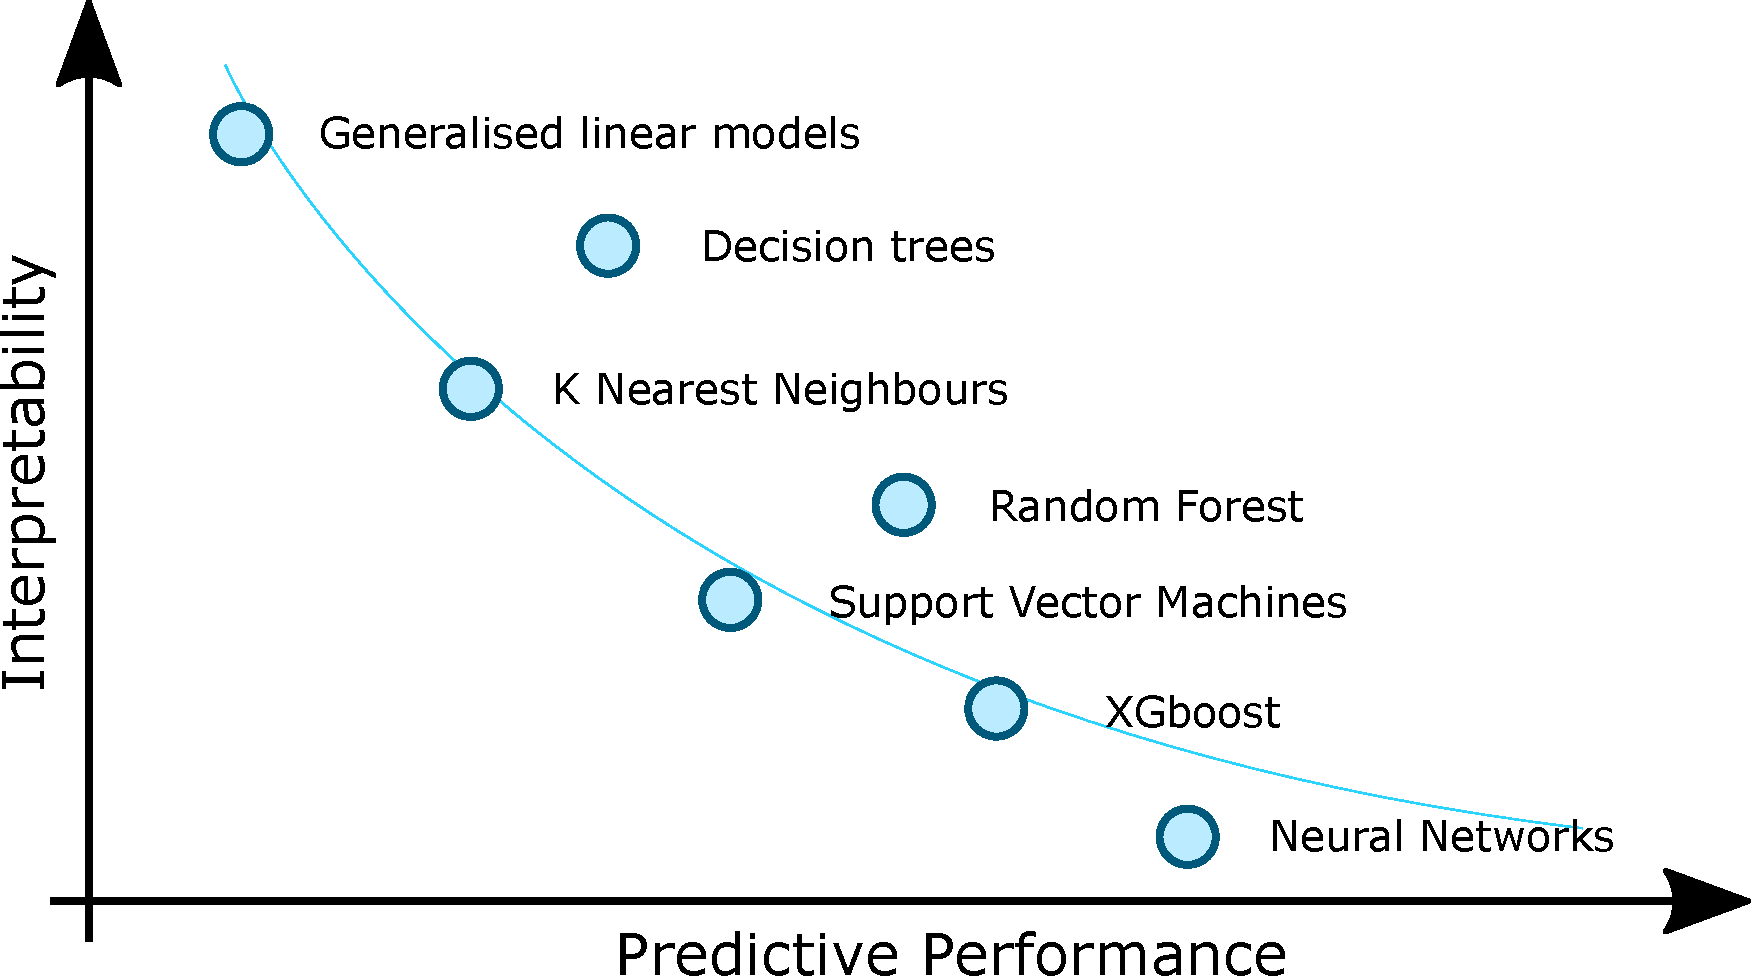
\includegraphics[width=0.9\textwidth]{figures/interpretability-performance-tradeoff}
    \caption[Performance vs. interpretability trade-off]{
        %
        Trade-off between predictive performance and interpretability in common sub-symbolic predictors.
        %
        The figure illustrates how different predictor families balance these two aspects, with simpler models being more interpretable but potentially less accurate.
        %
    }
    \label{fig:performance-vs-interpretability}
\end{figure}
%
The \emph{complexity} of a sub-symbolic predictor can vary significantly.
%
By complexity we mean the overall structure of the model, including the number of parameters, the operations that are performed, and possibly the way the model is trained.
%
\Glspl{DT}, for example, are relatively simple models that can be easily interpreted by humans.
%
The downside of \glspl{DT} is that they make predictions by linearly partitioning the input space, which can lead to poor generalisation on unseen data.
%
On the other hand, \glspl{NN} can be extremely complex, with millions of parameters and intricate architectures that are difficult to interpret.
%
However, \glspl{NN} can capture highly non-linear relationships in the data, often leading to superior predictive performance compared to simpler models.
%
The definition of interpretability is not univocal, and it lacks measures that are widely accepted~\cite{DBLP:journals/natmi/Rudin19}.
%
Despite that, \Cref{fig:performance-vs-interpretability} illustrates in an informal way the trade-off between predictive performance and interpretability in sub-symbolic predictors.


\subsection{\Glsentrylongpl{DT}}\label{subsec:decision-trees}

\subsection{\Glsentrylongpl{RF}}\label{subsec:random-forests}

\subsection{\Glsentrylongpl{SVM}}\label{subsec:svm}

\subsection{\Glsentrylongpl{NN}}\label{subsec:neural-networks}

\subsection{Limits of sub-symbolic \Gls{AI}}\label{subsec:limits-of-sub-symbolic-ai}
%! Author = matteomagnini
%! Date = 05/03/25

%----------------------------------------------------------------------------------------
\chapter{Neuro-symbolic AI}
\label{ch:nesy-ai}
\minitoc
%----------------------------------------------------------------------------------------

The origins of \gls{NeSy} \gls{AI} can be traced back to the 1950s and 1960s, during the early days of \gls{AI} research~\cite{Youheng_2023}.
%
At that time, the focus was on developing systems based on symbolic reasoning and rule-based problem-solving.
%
However, by the 1980s, the limitations of purely symbolic approaches became evident.
%
For instance, symbolic \gls{AI} struggled with tasks such as \gls{NLP} and computer vision, where the complexity of real-world data posed significant challenges.
%
To address these shortcomings, researchers began incorporating principles inspired by neuroscience into \gls{AI} systems.
%
This shift marked the beginning of efforts to integrate sub-symbolic methods, such as neural networks, into the field.

In the early 21st century, the idea of combining symbolic reasoning with neural networks gained traction.
%
This led to the emergence of \gls{NeSy} \gls{AI}, a hybrid approach that leverages the strengths of both symbolic and sub-symbolic paradigms.


\Gls{NeSy} \gls{AI} has since been applied to a wide range of domains, including healthcare, robotics, and \gls{NLP}.
%
It represents one of the most promising directions in \gls{AI} research, aiming to create systems capable of both learning from data and reasoning logically, much like humans.
%
The ``neuro'' component of \gls{NeSy} \gls{AI} is inspired by the human brain's ability to process information and learn from experience.
%
This is achieved through the use of neural networks, which enable the system to adapt and generalize from data.
%
On the other hand, the ``symbolic'' component relies on logical reasoning and structured representations of knowledge.
%
This allows the system to perform tasks such as deductive reasoning and to represent knowledge in a human-interpretable form, using symbols and rules.
%
By combining these two components, \gls{NeSy} \gls{AI} aims to overcome the limitations of purely symbolic or sub-symbolic approaches.
%
It enables the development of intelligent systems that can reason, learn, and adapt in complex environments.


According to a recent survey~\cite{DBLP:journals/nca/BhuyanRTS24} there exist at least six different types of integrating symbolic \gls{AI} and sub-symbolic \gls{ML} predictors.
%
Approaches to \gls{NeSy} can be categorised w.r.t. how the connectionist and symbolic components are integrated.
%
\begin{enumerate}
    \item \emph{Symbolic neuro-symbolic} (Type 1): utilizes neural networks for representational learning, which subsequently feeds into symbolic logic and inference mechanisms.
    %
    This approach is particularly effective in tasks such as language translation and classification, where neural-based semantic representations enhance symbolic reasoning;
    %
    \item \emph{symbolic[neuro]} (Type 2): incorporates neural networks as subcomponents within predominantly symbolic frameworks.
    %
    This integration improves pattern recognition capabilities within symbolic reasoning systems;
    %
    \item \emph{neuro|symbolic} (Type 3): involves a collaborative interaction between neural and symbolic components, which remain distinct and separate.
    %
    This type of integration is commonly applied in reinforcement learning and probabilistic logic systems;
    %
    \item \emph{neuro-symbolic$\rightarrow$neuro} (Type 4): embeds symbolic knowledge directly into neural network architectures or training processes.
    %
    This influences the decision-making and learning pathways of the neural networks;
    %
    \item \emph{neuro-symbolic} (Type 5): encodes symbolic constraints within neural architectures, often using soft logic constraints to directly affect neural computations;
    %
    \item \emph{neuro[symbolic]} (Type 6): represents a deeply integrated approach where symbolic reasoning capabilities are embedded directly within neural architectures.
    %
    However, achieving robust combinatorial reasoning in this type remains a significant challenge.
    %
\end{enumerate}

In the rest of this chapter, we focus on two sub-fields of \gls{NeSy} \gls{AI} -- namely \gls{SKI} and \gls{SKE} -- that cannot be mapped into a fixed one-to-one correspondence with the six types of integration above.
%
\Gls{SKI} and \gls{SKE} are two popular way to integrate symbolic \gls{AI} and sub-symbolic \gls{ML} predictors.
%
In the literature, there are hundreds of works that propose methods for these two tasks coming from different communities.
%
Here, we present both \gls{SKI} and \gls{SKE} in a unified way, providing a clear taxonomy of the methods, their properties, and their limitations.
%
What follows is a re-elaboration of the result of an \gls{SLR} that we conducted on the two topics: \emph{Symbolic Knowledge Extraction and Injection with Sub-symbolic Predictors: A Systematic Literature Review}~\cite{DBLP:journals/csur/CiattoSAMO24}.
%
\note{TODO: consider to add a brief explanation about in which type of integration \gls{SKI} and \gls{SKE} fit.}


\section[Symbolic knowledge injection]{\Glsentrylong{SKI}}\label{sec:ski}
%
\Gls{SKI} is a wide sub-field of \gls{NeSy}, which encompasses all the methods that in some way \emph{inject} symbolic knowledge into sub-symbolic predictors.
%
More precisely, we define \gls{SKI} as:
%
\begin{definition}[\gls{SKI}]
    \label{def:ski}
    any \textbf{algorithmic} procedure affecting how sub-symbolic predictors draw their inferences in such a way that predictions are either \textbf{computed} as a function of, or made \textbf{consistent} with, some given symbolic knowledge~\cite{DBLP:journals/csur/CiattoSAMO24}.
\end{definition}
%
We adopt this broad definition because the amount of works in the literature is vast and varied, furthermore the contributions come from different communities (e.g., \gls{ML}, \gls{AI}, \gls{NLP}, \gls{XAI}, logics, etc.), and they often use different terminologies.
%
This definition highlights several key aspects of \gls{SKI} that merit further discussion.
%
\gls{SKI} is conceptualized as a class of algorithms, and it involves procedures that take symbolic knowledge as input and produce \gls{ML} predictors as output.

Regarding the inputs of \gls{SKI} procedures, the primary requirement is that the knowledge must be symbolic and provided by the user, ensuring it is human interpretable.
%
Additionally, since the knowledge must be processed algorithmically, it is implicitly required to be machine interpretable.
%
This necessitates the use of formal languages, such as \gls{FOL} or decision trees, for knowledge representation, while avoiding free text or natural language.

Another implicit requirement is that the input knowledge must align functionally with the task of the predictor undergoing injection.
%
For instance, if a predictor is designed to classify customer profiles as either creditworthy or un-creditworthy, the symbolic knowledge should encode decision rules that serve the same purpose and utilize the same input features.

In terms of outcomes, \gls{SKI} procedures can be categorized into two non-exclusive scenarios.
%
First, they may enable sub-symbolic predictors to accept symbolic knowledge as input.
%
This is achieved through pre-processing algorithms that encode symbolic knowledge into sub-symbolic forms, allowing predictors to compute predictions based on this knowledge.
%
Second, \gls{SKI} procedures may modify sub-symbolic predictors to ensure their predictions are consistent with the symbolic knowledge.
%
This involves altering the structure or training process of the predictors so that they incorporate the symbolic knowledge into their inference process.
%
Regardless of the specific outcome, \gls{SKI} procedures are typically applied during the early stages of the \gls{ML} workflow, influencing both pre-processing and training phases.

Consistency plays a central role in \gls{SKI}.
%
To measure this, a consistency score is used to evaluate how effectively the predictor utilizes the injected knowledge in relation to the domain and task it was trained for.
%
For example, if a knowledge base specifies that loans should be granted to individuals from a specific minority group if their annual income exceeds a certain threshold, the predictor should generate predictions that adhere to this rule or minimize violations of it.

In the rest of this thesis, we will refer to \emph{uneducated predictor} to indicate a sub-symbolic predictor that does not use symbolic knowledge -- i.e., before the injection takes place --, and to \emph{educated predictor} to indicate a sub-symbolic predictor that uses symbolic knowledge---i.e., after the injection takes place.
%
Sometimes, in the literature the term \emph{enriched predictor} is also used instead of \emph{educated predictor}.


\subsection{Motivations and goals}\label{subsec:ski-motivations-and-goals}
%
\Gls{SKI} can be used for several reasons, such as:
%
\begin{inlinelist}
    %
    \item \label{itm:prediction}\emph{improving the model's predictive performance}, by leveraging symbolic knowledge to guide their learning or inference;
    %
    \item \label{itm:interpretability}\emph{improving the model's interpretability}, by making their predictions consistent with symbolic knowledge;
    %
    \item \label{itm:robustness}\emph{increase the robustness} of sub-symbolic predictors, by making them less sensitive to data perturbations (e.g., noise, data scarcity, etc.);
    %
    \item \label{itm:complexity}\emph{reduce the model complexity} of the models, by shaping their structure or by constraining their parameters;
    %
    \item and possibly many more.
    %
\end{inlinelist}


\Cref{itm:prediction} is one of the most common motivations for \gls{SKI}.
%
The idea is simple: if there is already some (symbolic) knowledge about a particular domain or task, then it is reasonable to expect that the predictor can benefit from it.
%
In this way the model learns both from the data -- inductively -- and from the symbolic knowledge---mimicking deductive reasoning.


Another common reason to use \gls{SKI} is to increase the \emph{interpretability} of the model, as stated in \Cref{itm:interpretability}.
%
In the context of \gls{XAI}, this is usually referred as \gls{XAI} \emph{by design} (\Cref{par:xai-by-design}).
%
The intuition is simple: the model is made to be consistent -- up to a certain extent -- with the symbolic knowledge, which is usually more interpretable than the model itself.
%
This can be done in two ways: either by using \emph{symbols as constraints} or by \emph{transparent box design}.
%
More details about these two approaches are provided in \Cref{par:guided-learning} and \Cref{par:structuring}, respectively.


Predictive performances and \gls{XAI} are the main motivations for \gls{SKI}, but not the only ones.
%
The \emph{robustness} (\Cref{itm:robustness}) of a predictive model is another important challenge~\cite{DBLP:conf/eccv/LiuCZH18}, and it relates to predictors' ability to maintain performance despite the presence of input perturbations.
%
A metric of robustness in the context of \gls{SKI} is defined in the work ``An Empirical Study on the Robustness of Knowledge Injection Techniques Against Data Degradation''~\cite{DBLP:conf/woa/RafanelliMACO24}.
%
The content of the paper is presented in~\Cref{sec:empirical-study-on-the-robustness-of-ski-methods}.
%
Along with robustness, there are other metrics -- often neglected -- that play a crucial role in the design of intelligent systems, such as \emph{memory footprint} (\Cref{itm:complexity}), \emph{latency}, data efficiency, and so on.
%
These \gls{QoS} metrics are presented in the work ``Symbolic Knowledge Injection Meets Intelligent Agents: QoS metrics and experiments''~\cite{DBLP:journals/aamas/AgiolloRMCO23}, which is discussed in~\Cref{sec:ski-meets-intelligent-agents}.


\subsection{What to inject}\label{subsec:what-to-inject}
%
\begin{figure}
    \centering
    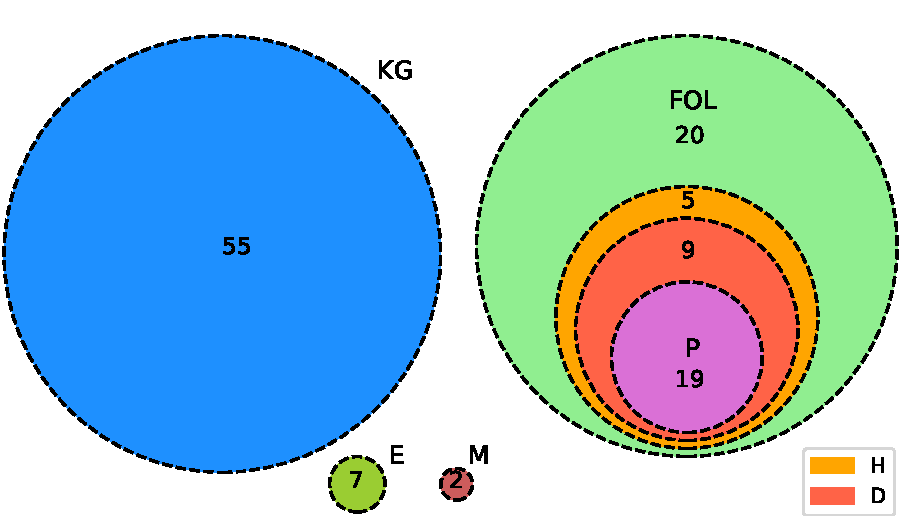
\includegraphics[width=.6\linewidth]{figures/ski-logic}
    \caption[Venn diagram categorising SKI methods w.r.t. the input knowledge]{
        Venn diagram categorising SKI methods w.r.t.\ the \emph{input knowledge} type: knowledge graphs (KG), propositional logic (P), first-order logic (FOL), expert knowledge (E), Datalog (D), Horn logic (H), or modal logic (M).
        %
        The image is taken from~\cite{DBLP:journals/csur/CiattoSAMO24} and it refers to 117 surveyed \gls{SKI} methods.
    }
    \label{fig:pie-ski-logic}
\end{figure}
%
\note{ERROR: there is an inconsistency between this image and \Cref{fig:venn-diagram-logics}. P here is subset of D, there it is not.}
%
A key distinction in \gls{SKI} methods lies in whether the chosen formalism is \emph{machine interpretable}, \emph{human interpretable}, or both.
%
\Gls{SKI} methods can be categorized into two primary groups based on the formalism used to represent input knowledge~\cite{DBLP:journals/csur/CiattoSAMO24}:
%
\begin{itemize}
    \item \textbf{Logic formulas or \glspl{KB}:} These adhere to \gls{FOL} or its subsets, making them interpretable by both humans and machines.
    %
    The sub-categories, ordered by decreasing expressiveness, include:
    %
    \begin{itemize}
        %
        \item \emph{\gls{FOL} formulas:} These encompass recursive terms, variables, predicates of any arity, and various logic connectives, potentially expressing definitions.
        %
        \item \emph{Horn logic:} Often referred to as Prolog-like logic, this formalism consists of head–body rules involving predicates and terms of any kind.
        %
        \item \emph{Datalog:} A restricted subset of Horn logic that excludes recursive terms, allowing only constants or variables as terms.
        %
        \item \emph{Modal logics:} These extend the above logics with modal operators (e.g., \(\square\) and \(\lozenge\)), which express modalities such as necessity or possibility.
        %
        \item \emph{Knowledge graphs:} A practical application of description logics designed to represent entity–relation graphs.
        %
        \item \emph{Propositional logic:} This involves Boolean variables and logical connectives, offering a simpler yet effective formalism.
    \end{itemize}
    %
    \item \textbf{Expert knowledge:} This category includes human-interpretable knowledge that is not inherently machine-readable.
    %
    Examples include physics equations, syntactical rules, or domain-specific expertise.
    %
    Since expert knowledge is not directly machine interpretable, it often requires transformation into tensorial form through data generation, a process that typically involves human engineers and can be labor-intensive.
\end{itemize}
%
\Cref{fig:pie-ski-logic} illustrates the distribution of surveyed \gls{SKI} methods based on their formalism of choice.
%
\Glspl{KG} emerge as the most prevalent category, representing nearly half of the surveyed methods.
%
In contrast, modal logics constitute the smallest group.
%
Methods based on \gls{FOL} or its subsets (excluding \glspl{KG}) form another significant cluster, with propositional logic being particularly prominent due to its relative simplicity and widespread use.
%
The specific logic formalism employed in the surveyed papers is reported where available.
%
However, this information is rarely explicitly stated by the authors.
%
Instead, the logic is often inferred from the constraints and descriptions provided in the respective works.

Practical examples of symbolic knowledge that can be injected into sub-symbolic predictors are the public health guidelines on type-2 diabetes of the National Institute of Diabetes and Digestive and Kidney Diseases\footnote{\url{https://www.niddk.nih.gov/health-information/diabetes/}}.
%
These guidelines have been encoded into logic formulas~\cite{DBLP:conf/pkdd/KunapuliBSMS10} and used in works related to \gls{SKI}~\cite{Magnini-telmed2025}.
%
The first guideline state that if a patient has a glucose value greater or equal to 125 mg/dL and a \gls{BMI} greater or equal to 30, then the patient is considered diabetic.
%
The second one says that if a patient has a glucose value lower or equal to 100 mg/dL and a \gls{BMI} lower or equal to 25, then the patient is considered non-diabetic.
%
In \gls{FOL}, the first statement can be encoded as:
%
\begin{equation}\label{eq:rule-diabetic}
  \forall x . ( \text{glucose}(x) \geq 125 \land \text{bmi}(x) \geq 30 \rightarrow \text{Diabetic}(x))
\end{equation}
%
whereas the second statement can be encoded as:
%
\begin{equation}\label{eq:rule-not-diabetic}
  \forall x . ( \text{glucose}(x) \leq 100 \land \text{bmi}(x) \leq 25 \rightarrow \neg \text{Diabetic}(x))
\end{equation}


\subsection{Where to inject}\label{subsec:where-to-inject}
%
\begin{figure}
    \centering
    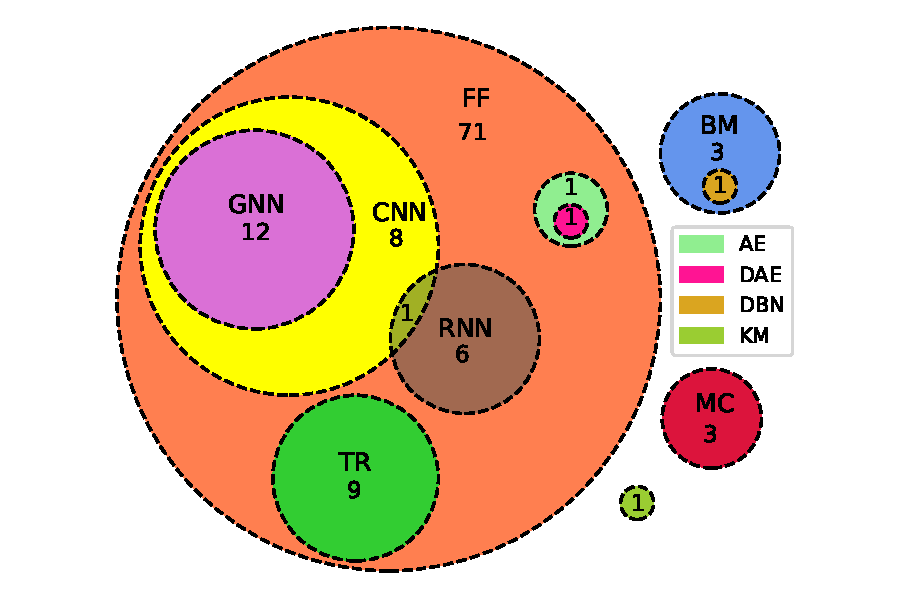
\includegraphics[width=.6\linewidth]{figures/ski-predictors}
    \caption[Venn diagram categorising SKI methods w.r.t. the predictor type]{
        Venn diagram categorising \gls{SKI} methods w.r.t.\ the type of sub-symbolic predictor: feed-forward (FF), convolutional (CNN), graph (GNN) or recurrent (RNN) neural networks, Boltzmann machines (BM), Markov chains (MC), transformers (TR), auto-encoders (AE), deep belief networks (DBN), denoising auto-encoders (DAE), kernel machines (KM).
        %
        The image is taken from~\cite{DBLP:journals/csur/CiattoSAMO24} and it refers to 117 surveyed \gls{SKI} methods.
    }
    \label{fig:pie-ski-predictors}
\end{figure}
%
\Gls{SKI} methods can target many different types of sub-symbolic predictors.
%
The vast majority of them are \glspl{NN}.
%
Among \glspl{NN}, there are different kinds of architectures that one can use to inject symbolic knowledge including.
%
In addition to \glspl{NN}, \gls{SKI} methods can also target other types of sub-symbolic predictors.
%
The predictors targeted by the surveyed \gls{SKI} methods are:
%
\begin{itemize}
    \item \textbf{feed-forward NNs} multi-layered \glspl{NN} in which neurons from layer i are only connected with layer i + 1, and multiple ($\ge$ 2) layers may exist;
    %
    \item \textbf{convolutional NNs} (CNNs) particular case of FF, \glspl{NN} that use convolutional layers to extract features from the input data, typically used in computer vision tasks;
    %
    \item \textbf{graph NNs} (GNNs) particular case of \glspl{CNN}, \glspl{NN} that operate on graph-structured data, allowing for the injection of symbolic knowledge in the form of graph structures;
    %
    \item \textbf{recurrent NNs} (RNNs) \glspl{NN} that use recurrent connections to process sequential data, such as time series or natural language;
    %
    \item \textbf{transformers} (TR) a type of \glspl{NN} architecture that uses self-attention mechanisms to process sequences, widely used in natural language processing tasks;
    %
    \item \textbf{auto-encoders} (AE) a type of \glspl{NN} that learns to encode input data into a lower-dimensional representation and then decode it back to the original input, often used for dimensionality reduction or feature extraction;
    %
    \item \textbf{denoising auto-encoders} (DAE) a type of auto-encoder that learns to reconstruct the original input from a corrupted version, often used for noise reduction or data augmentation;
    %
    \item \textbf{Boltzmann machines} (BM) a type of stochastic \glspl{NN} that can learn complex distributions over their inputs, often used for generative tasks;
    %
    \item \textbf{Markov chains} (MC) probabilistic models that represent systems that transition between states based on certain probabilities, often used for sequence prediction;
    %
    \item \textbf{deep belief networks} (DBN) a type of generative model that consists of multiple layers of stochastic, latent variables, often used for unsupervised learning tasks;
    %
    \item \textbf{kernel machines} (KM) a type of sub-symbolic predictor that uses kernel functions to map input data into a higher-dimensional space, allowing for non-linear decision boundaries.
\end{itemize}
%
\Cref{fig:pie-ski-predictors} illustrates the distribution of surveyed \gls{SKI} methods based on the type of sub-symbolic predictor they target.

One reason why the vast majority of methods rely on \glspl{NN} is straightforward: methods tailored to \glspl{GNN} (resp., \glspl{CNN}) assume the networks to accept specific kinds of data as input, e.g., graphs (resp., images), while ordinary feed-forward \glspl{NN} accept raw vectors of real numbers.
%
Another reason is that \glspl{NN} are the most popular sub-symbolic predictors in the \gls{ML} community, and they are often used as a default choice for many tasks.
%
Finally, \glspl{NN} are highly flexible and easy to manipulate, making them ideal for \gls{SKI} methods.


\subsection{How to inject}\label{subsec:how-to-inject}
%
\begin{SCfigure}
    \centering
    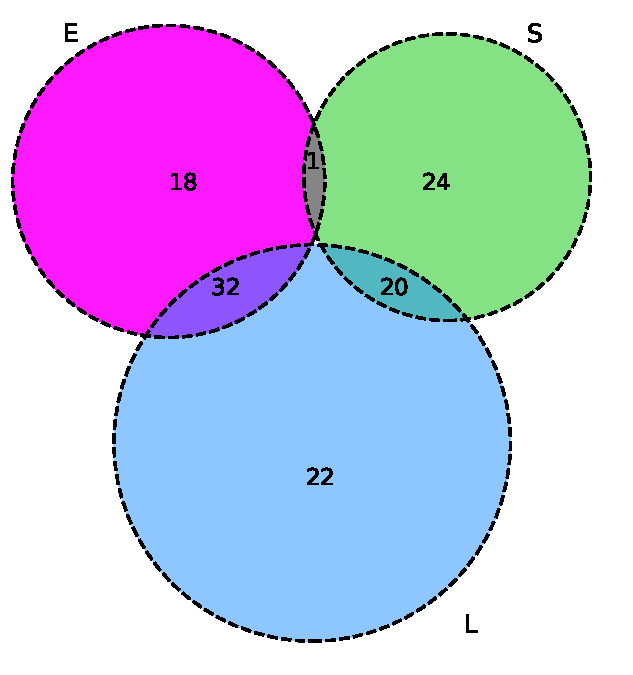
\includegraphics[width=.4\linewidth]{figures/ski-integration}
    \caption[Venn diagram categorising SKI methods]{
        Venn diagram categorising SKI methods w.r.t.\ the \emph{injection} strategy type: structuring (S), embedding (E), or guided learning (L).
        %
        The image is taken from~\cite{DBLP:journals/csur/CiattoSAMO24} and it refers to 117 surveyed \gls{SKI} methods.
    }
    \label{fig:pie-ski-injection}
\end{SCfigure}
%
How can symbolic knowledge, such as the ones in \Cref{eq:rule-diabetic,eq:rule-not-diabetic}, be injected into sub-symbolic predictors?
%
To answer this question, scientists have designed several strategies, which can be broadly grouped into three main categories~\cite{DBLP:journals/csur/CiattoSAMO24}: structuring, guided learning, and embedding.
%
It may occur that a method uses more than one strategy at a time.
%
\Cref{fig:pie-ski-injection} illustrates the distribution of surveyed \gls{SKI} methods based on their strategy of choice.
%
The survey revealed that all three strategies are widely used, with learning being the most frequent but not dominant.

The main entities involved in the \gls{SKI} process -- and that are common to virtually all \gls{SKI} methods -- are:
%
\begin{itemize}
    %
    \item \textbf{symbolic knowledge:} in the vast majority of cases, this is a set of logic formulas or a \gls{KB} that encodes the symbolic knowledge to be injected;
    %
    \item \textbf{parsed knowledge:} a syntactic structure that represents the \emph{parsed} symbolic knowledge, often in the form of a \gls{AST} or graph;
    %
    \item \textbf{sub-symbolic component:} a sub-symbolic instance built upon the parsed symbolic knowledge;
    %
    \item \textbf{uneducated sub-symbolic predictor:} a sub-symbolic predictor that has not been enriched with the symbolic knowledge;
    %
    \item \textbf{educated sub-symbolic predictor:} the final sub-symbolic predictor that has been enriched with the symbolic knowledge.
    %
\end{itemize}
%


\paragraph{Structuring}\label{par:structuring}
%
\begin{figure}
    \centering
    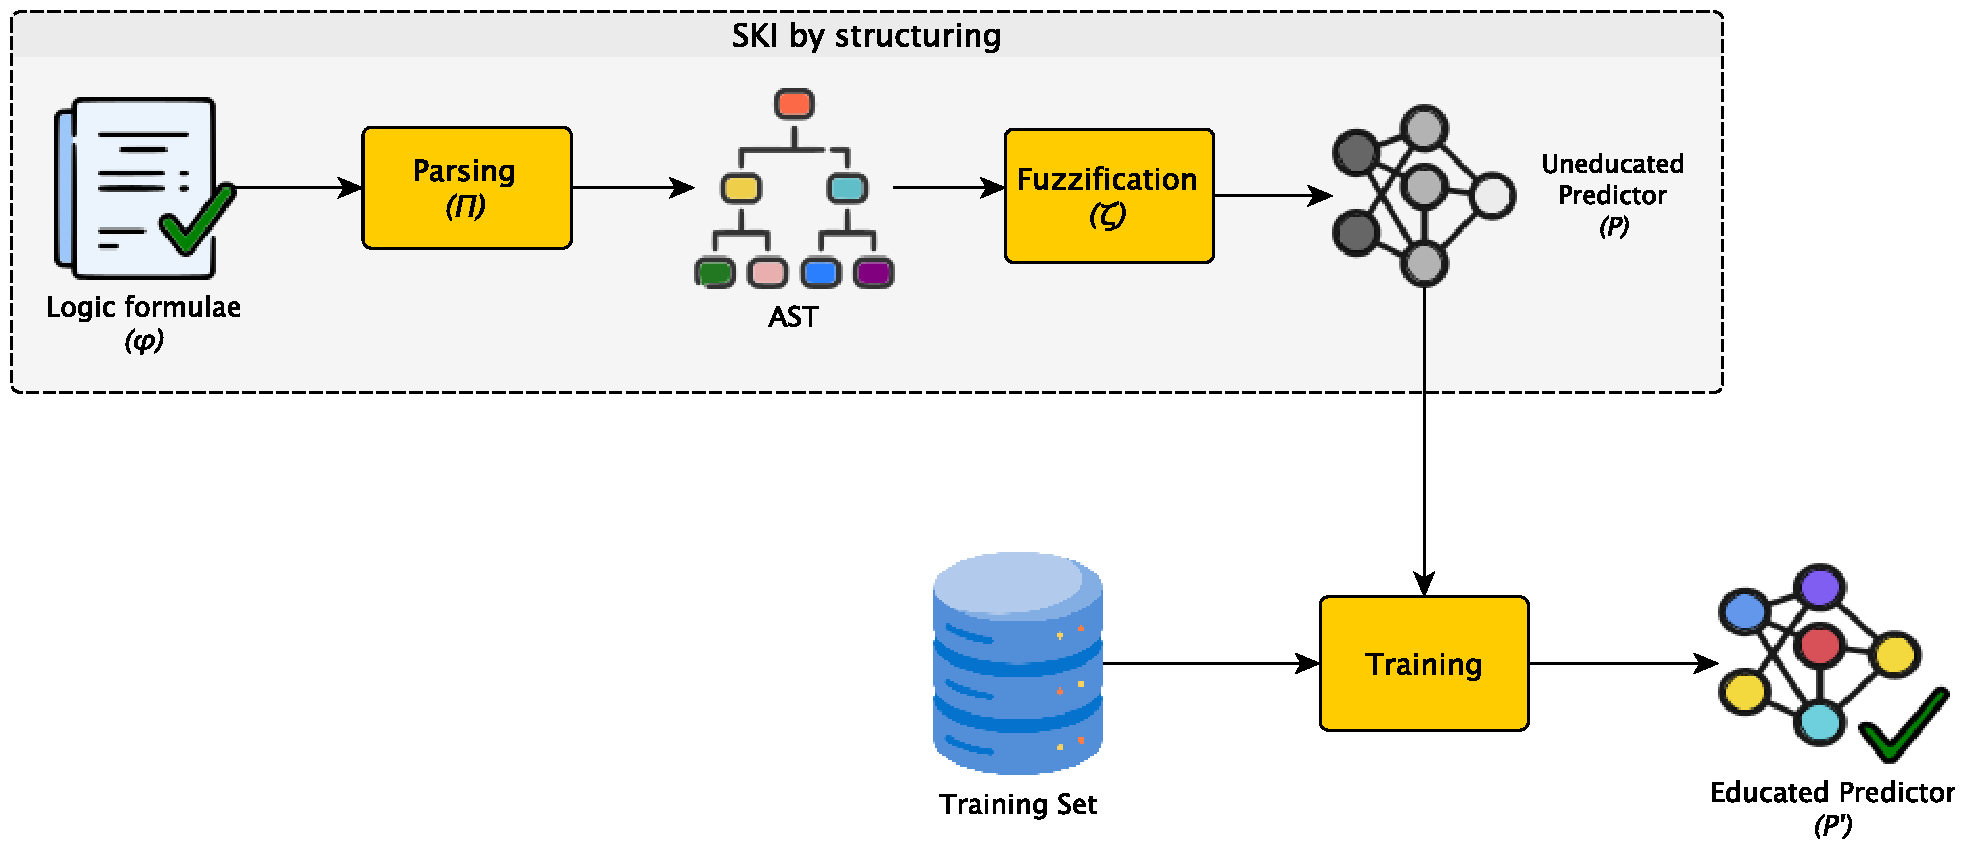
\includegraphics[width=.9\linewidth]{figures/workflow-structuring}
    \caption[SKI workflow of structuring strategy]{
        Workflow of the structuring strategy.
        %
        The symbolic knowledge is parsed and used to create a sub-symbolic predictor -- or part of it -- that mimics the symbolic knowledge.
        %
        The resulting predictor is then trained on data, if needed.
    }
    \label{fig:workflow-structuring}
\end{figure}
%
By predictor structuring, or simply structuring, we identify all those methods that use a part (or the whole) of a sub-symbolic predictor to \emph{mirror} the symbolic knowledge via its own internal structure.
%
A predictor is either created or extended to mimic the behavior of the symbolic knowledge.
%
For instance, when the predictors are \glspl{NN}, their internal structure is crafted to represent logic predicates via neurons, and logic connectives via synapses.
%
\Cref{fig:workflow-structuring} illustrates the workflow of the structuring strategy.
%
Usually, in the structuring strategy, the symbolic knowledge is in the form of logic formulas ($\phi$) (e.g., subsets of \gls{FOL}).
%
The formulas are then parsed into a syntactic structure (e.g., \gls{AST}).
%
At this point, a \emph{fuzzification} ($\zeta$) step is performed to convert the \emph{boolean} (also the term \emph{crisp} is used in the literature) -- because a logic predicate is either \emph{true} or \emph{false} -- symbolic knowledge into a \emph{fuzzy} interpretation of it, which is more suitable for sub-symbolic predictors.
%
This fuzzy interpretation is often \emph{continuous} and bounded to a predefined range, such as \([0, 1]\).
%
The property of continuity is a key requirement for training sub-symbolic structures via gradient descent (e.g., \glspl{NN} or part of them).
%
In practice, $\zeta$ is implemented as a mapping function that transforms logic operators into continuous functions (e.g., see \Cref{subsec:kill-fuzzifier,subsec:kins-fuzzifier}).
%
The result of the fuzzification process is an \emph{uneducated} predictor ($P$) that is then trained on the training set.
%
After the training, the predictor is now \emph{educated} ($P'$) and can be used to make predictions on the test set or in production.
%

\paragraph{Guided learning}\label{par:guided-learning}
%
\begin{figure}
    \centering
    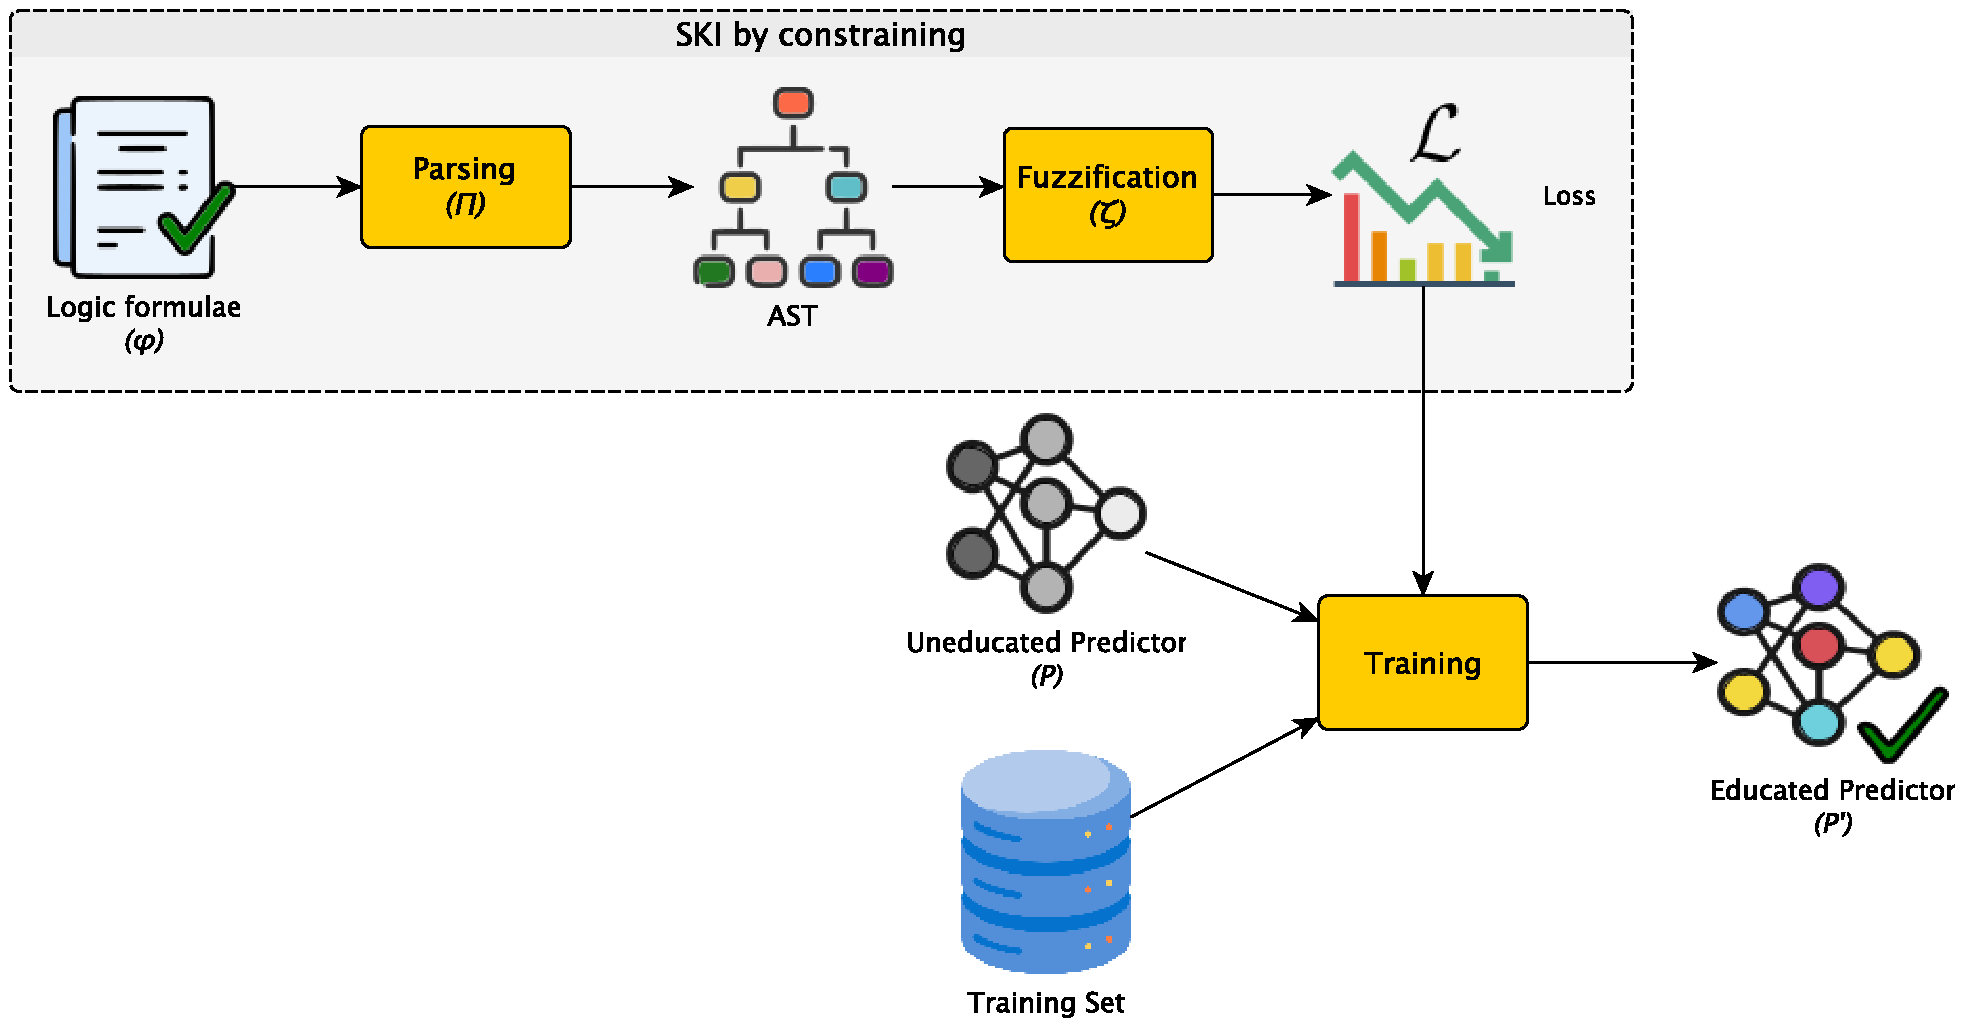
\includegraphics[width=.9\linewidth]{figures/workflow-constraining}
    \caption[SKI workflow of guided learning strategy]{
        \gls{SKI} workflow of the guided learning strategy.
        %
        The symbolic knowledge is used to guide the training of a sub-symbolic predictor, which is then trained on data.
    }
    \label{fig:workflow-learning}
\end{figure}
%
By guided learning, we refer to all those methods that affect the sub-symbolic predictor's training process by using the symbolic knowledge as a \emph{constraint}/\emph{guidance}.
%
Usually, \gls{SKI} algorithms based on this strategy target sub-symbolic predictors that can be trained with gradient descent, such as \glspl{NN}.
%
\Cref{fig:workflow-learning} illustrates the workflow of the guided learning strategy.
%
Like in the case of structuring, the symbolic knowledge is parsed and fuzzified.
%
Differently from structuring, the result of the fuzzification process is not a subcomponent of the predictor's architecture (e.g., neurons, connections), but rather a set of continuous numeric functions.
%
Conceptually, these functions represent the degree of violation of the symbolic knowledge by the predictor's predictions.
%
The higher the degree of violation, the higher the value of the function.
%
The symbolic-derived functions are then included in the loss function of the predictor, which is then trained on the training set.
%
The combination between the ``classical'' loss function (e.g., cross-entropy, mean squared error, etc.) and the symbolic-derived functions can be done in many ways, but it is usually done via a weighted sum.


\paragraph{Embedding}\label{par:ski-embedding}
%
\begin{figure}
    \centering
    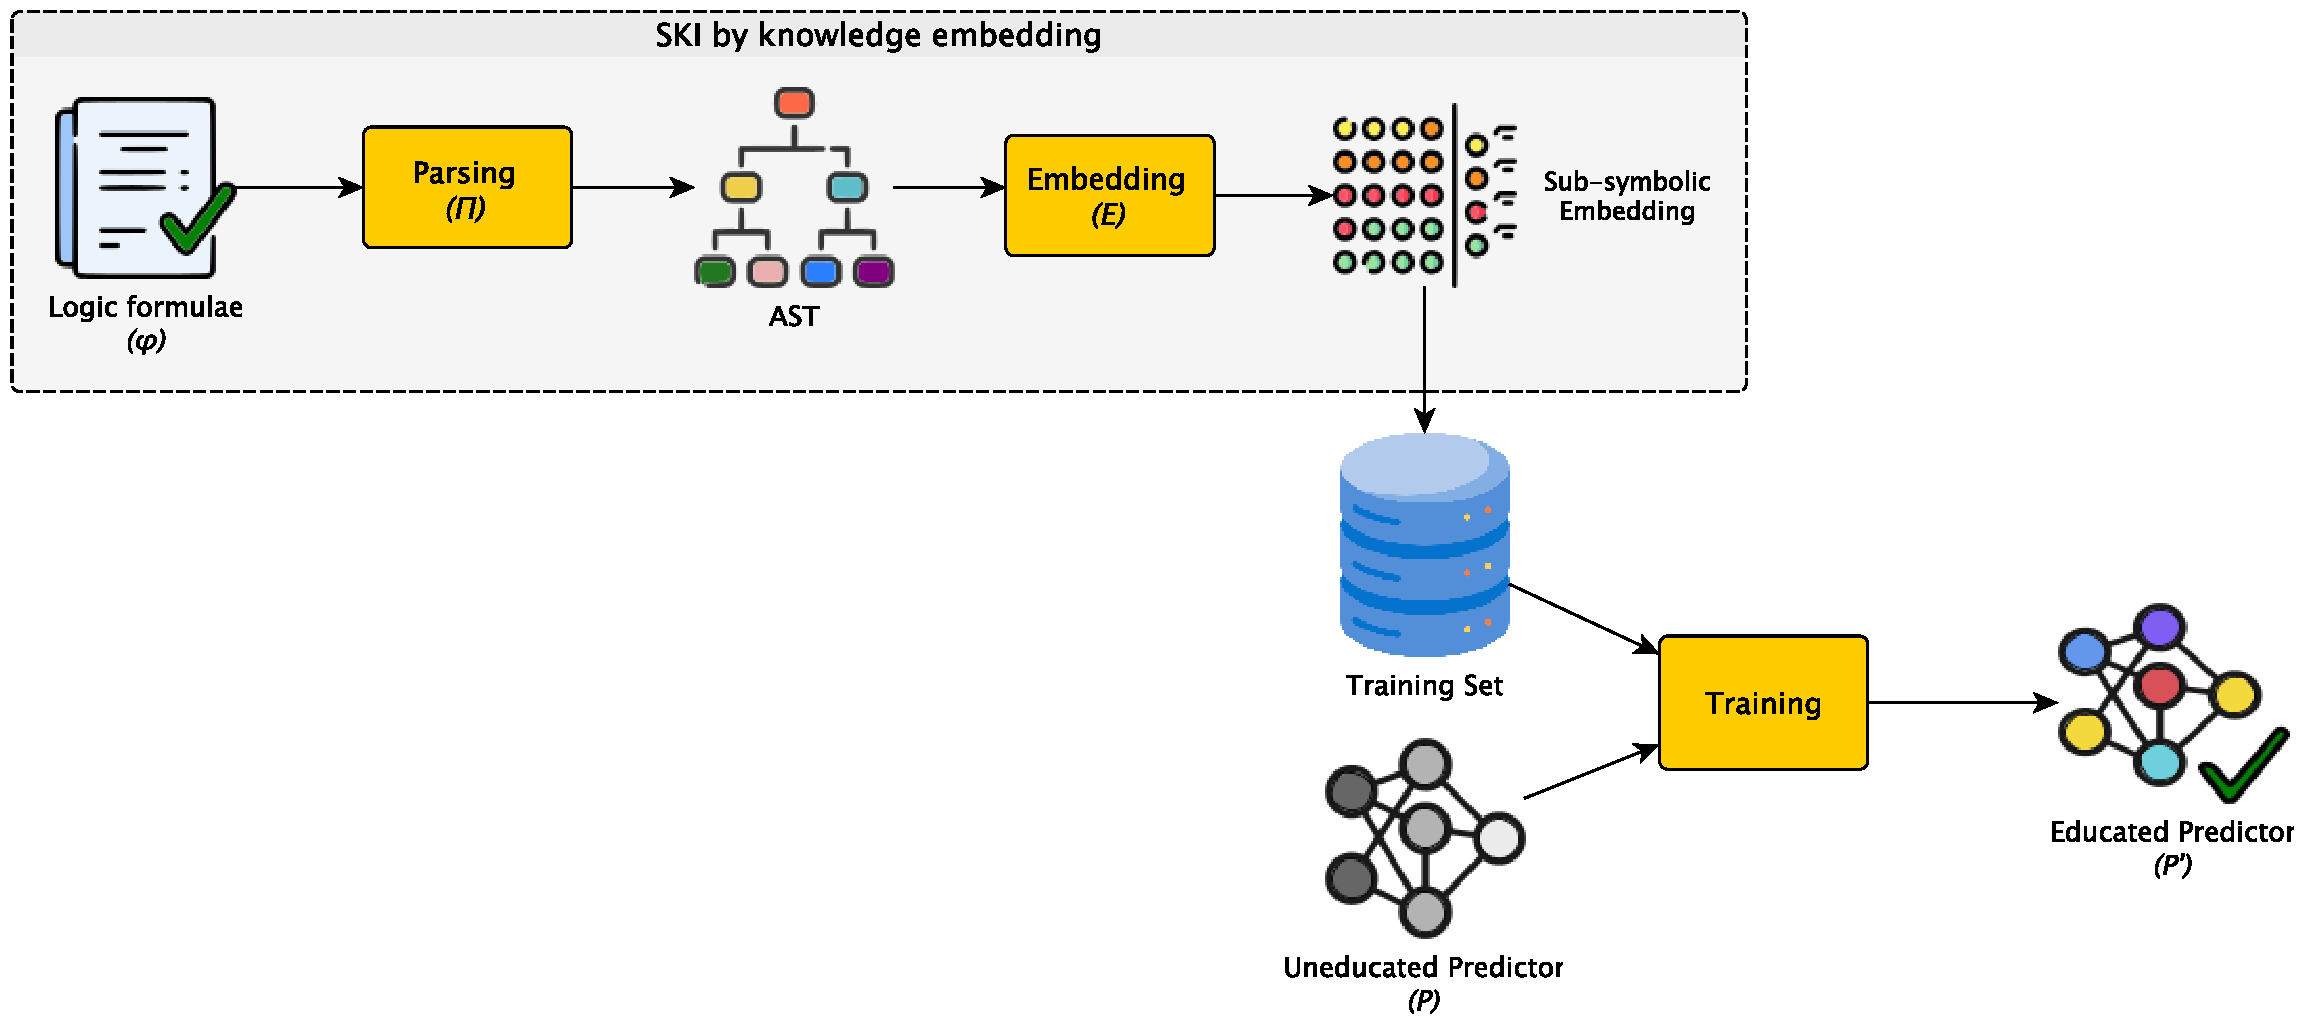
\includegraphics[width=.9\linewidth]{figures/workflow-embedding}
    \caption[SKI workflow of embedding strategy]{
        \gls{SKI} workflow of the embedding strategy.
        %
        The symbolic knowledge is parsed and embedded into a sub-symbolic predictor, which is then trained on data.
    }
    \label{fig:workflow-embedding}
\end{figure}
%
In the embedding strategy, the symbolic knowledge is converted -- i.e., \emph{embedded}-- into numeric-array representations.
%
\Cref{fig:workflow-embedding} illustrates the workflow of the embedding strategy.
%
The output of the fuzzification process is a set of numeric arrays (e.g., vectors, matrices, and tensors) that represent the symbolic knowledge.
%
These arrays are then provided as input to the sub-symbolic predictor.
%
This is the common strategy exploited by the \gls{KG}~\cite{DBLP:conf/ijcai/LambGGPAV20} embedding community as well as by \glspl{GNN}~\cite{DBLP:journals/tkde/WangMWG17}.


\subsection[Limitations and challenges of SKI]{Limitations and challenges of \Gls{SKI}}\label{subsec:limitations-and-challenges-of-ski}
%
Despite the numerous advantages of \gls{SKI}, there are several limitations and challenges that need to be addressed.
%
Here, we elicit the most common and relevant limitations and challenges of \gls{SKI} that we encountered in the literature:
%
\begin{itemize}
    %
    \item \textbf{Lack of generality}, many \gls{SKI} methods are tailored to domain-specific tasks.
    %
    Often, even if they are presented as general-purpose, their implementation is not and it requires significant effort to adapt them to different tasks or domains;
    %
    \item \textbf{Lack of reproducibility}, the experiments presented -- if any -- in the papers are often not reproducible.
    %
    This happens because the authors do not provide enough details about the implementation of the method (e.g., they do not mention the value of some key hyperparameters), or they do not share the code and data used in the experiments.
    %
    Only 49 out of 117 surveyed methods provide public code base for the experiments\footnote{\label{foot:supplementary}see Table B of the supplementary material of~\cite{DBLP:journals/csur/CiattoSAMO24}};
    %
    \item \textbf{Lack of availability}, the vast majority of \gls{SKI} methods is not available as open-source software.
    %
    Only 11 out of 117 surveyed methods provide a public library for the method$^{\ref{foot:supplementary}}$.
    %
    Authors usually do not mention any code base in their papers, and if they do, the code can lack the necessary dependencies, lack documentation, or it could have been removed from public repositories;
    %
    \item \textbf{Limits of the symbolic knowledge}, despite the variety of symbolic knowledge that can be injected (see \Cref{fig:pie-ski-logic}), there are still many limitations.
    %
    Indeed, the claimed expressiveness of the logic formalism supported by a method is often not fully exploited in practice.
    %
    In particular, \gls{FOL} allows for the representation of recursive terms, but most \gls{SKI} methods do not support them because of the target predictors.
    %
    Target predictors are almost always \glspl{NN}, which cannot support recursion in their architecture---modern \glspl{NN} are \glspl{DAG}.
    %
\end{itemize}

\section[Symbolic knowledge extraction]{\Glsentrylong{SKE}}\label{sec:ske}
%
\gls{SKE} is the process of extracting symbolic knowledge from sub-symbolic predictors.
%
Here, we provide the broad definition of \gls{SKE} that we adopt in this thesis:
%
\begin{definition}[\gls{SKE}]
    \label{def:ske}
    any \textbf{algorithmic} procedure accepting \textbf{trained} sub-symbolic predictors as input and producing \textbf{symbolic} knowledge as output so that the extracted knowledge reflects the behavior of the predictor with high \textbf{fidelity}~\cite{DBLP:journals/csur/CiattoSAMO24}.
\end{definition}
%
Once again, the definition is broad because the amount of contributions in the literature is vast and varied, they often use different terminologies and come from different communities.
%
\Gls{SKE} is conceptualized as a class of algorithms, which are finite-step procedures defined by their inputs and outputs.

The input to \gls{SKE} procedures must be trained \glspl{ML} predictors.
%
There are no restrictions on the type of predictor, meaning that \gls{SKE} methods can, in principle, be applied to any predictor family.
%
However, this requirement implies that the predictor must have already undergone training and achieved satisfactory performance for its intended task.
%
Thus, within an \gls{ML} workflow, \gls{SKE} is performed after the training and validation phases are complete.

The output of \gls{SKE} procedures is symbolic knowledge, which is broadly defined as human-intelligible information.
%
This can include logic formulas, decision trees, or even plain human-readable text.
%
For an algorithm to qualify as a valid \gls{SKE} procedure, the extracted knowledge must closely reflect the behavior of the original predictor within the domain it was trained for.
%
This fidelity is typically measured using a fidelity score, which evaluates how well the extracted knowledge replicates the predictor's behavior for the given task and domain.

The extracted knowledge should ideally function as a predictor itself, allowing it to be queried in the same way as the original predictor.
%
For example, if the original predictor is an image classifier, the extracted knowledge should enable an intelligent agent to classify similar images and produce equivalent results.
%
This agent could be either computational (e.g., a software program) or human, depending on whether the extracted knowledge is machine or human interpretable.
%
The use of logic-based knowledge as the target of \gls{SKE} is particularly advantageous, as it supports both machine and human interpretability.


\subsection{Motivations and goals}\label{subsec:ske-motivations-and-goals}
%
\Gls{SKE} serves multiple purposes, including:
%
\begin{inlinelist}
    %
    \item \label{itm:inspection} the inspection of the internal operations of opaque predictors, which are otherwise treated as black boxes,
    %
    \item \label{itm:automation} the automation and acceleration of the process of acquiring symbolic knowledge, eliminating the need for manually crafting \glspl{KB},
    %
    \item \label{itm:xai} providing valuable capabilities within the scope of \gls{XAI} to analyze black-box predictors.
\end{inlinelist}

\Cref{itm:inspection} is particularly important for understanding the behavior of opaque predictors.
%
By inspecting their internal operations, \gls{SKE} allows researchers and practitioners to identify patterns in mispredicted inputs or even detect correctly predicted patterns that rely on unethical or biased decision processes.
%
This capability is crucial for ensuring the ethical and transparent use of \gls{ML} systems, especially in sensitive domains such as healthcare or finance.

\Cref{itm:automation} highlights another key advantage of \gls{SKE}: the ability to automate the extraction of symbolic knowledge.
%
This eliminates the labor-intensive process of manually crafting \glspl{KB}, which often requires significant domain expertise and time.
%
By automating this process, \gls{SKE} not only accelerates knowledge acquisition but also enables the reuse of extracted knowledge across different tasks or systems, provided the knowledge is represented in a compatible format.

Finally, \Cref{itm:xai} emphasizes the role of \gls{SKE} in \gls{XAI}.
%
The extracted knowledge can be used to construct explanations for the behavior of black-box predictors, making their decision-making processes more interpretable.
%
In some cases, this knowledge may even serve as an interpretable surrogate model, replacing the original predictor if it achieves a high fidelity score~\cite{DBLP:conf/atal/CiattoCSO20}.
%
Additionally, \gls{SKE} enables the comparison of multiple black-box predictors performing the same task, highlighting their differences and commonalities.
%
It also facilitates the merging of knowledge extracted from various predictors, even if they belong to different families, as long as the same representation format is used~\cite{DBLP:conf/aiia/CiattoCOC19}.


\subsection{What to extract}\label{subsec:what-to-extract}
%
\begin{figure}
    \centering
    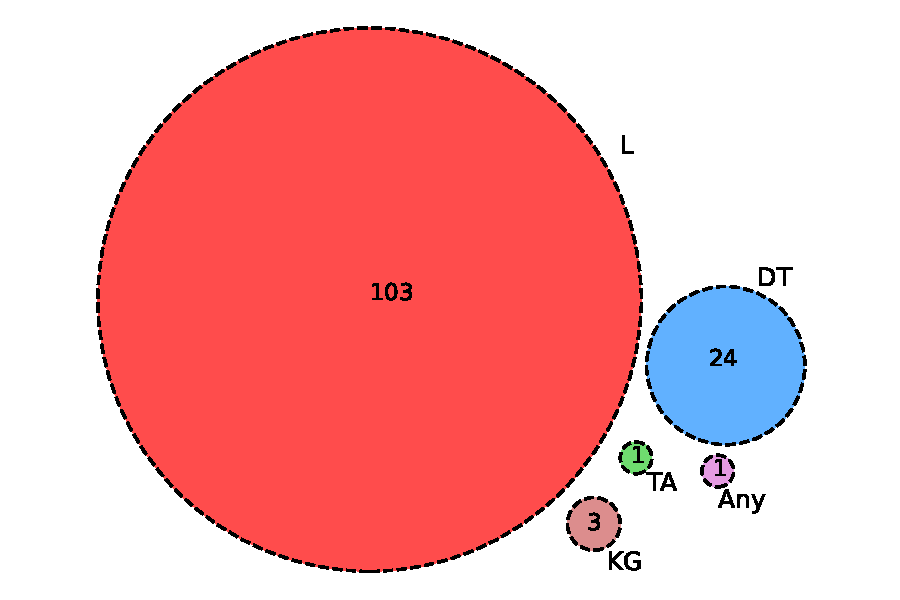
\includegraphics[width=.6\linewidth]{figures/ske-rule-shape}
    \caption[Venn diagram categorising SKE methods]{
        %
        Venn diagram categorising \gls{SKE} methods w.r.t.\ the \emph{shape} of the extracted symbolic knowledge: rule lists (L), decision trees (DT), decision tables (TA), or knowledge graphs (KG).
        %
        The image is taken from~\cite{DBLP:journals/csur/CiattoSAMO24} and it refers to 132 surveyed \gls{SKE} methods.
    }
    \label{fig:pie-ski-shape}
\end{figure}
%
\begin{figure}
    \centering
    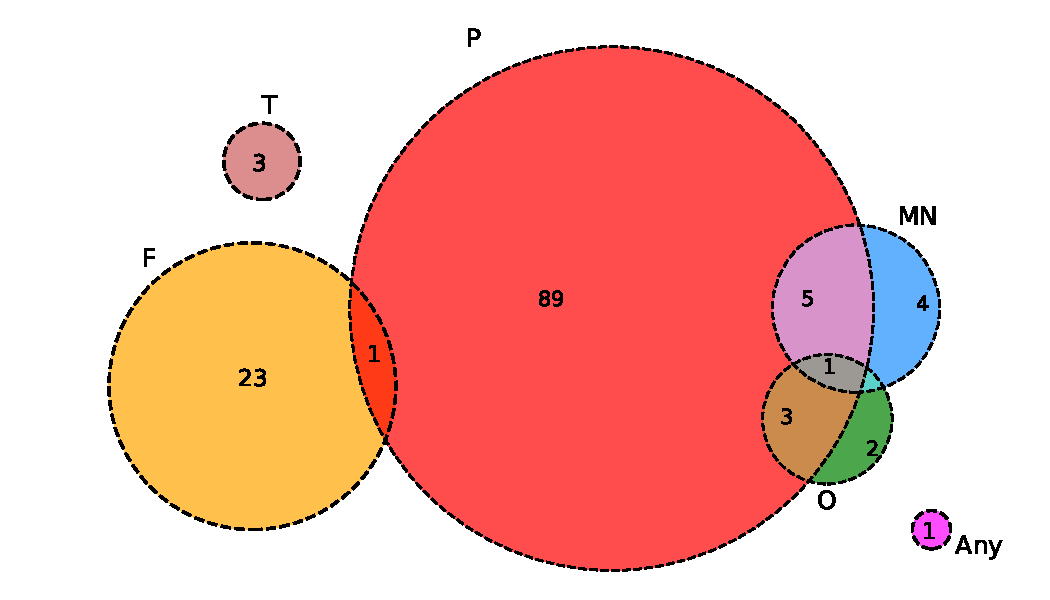
\includegraphics[width=.6\linewidth]{figures/ske-rule-format}
    \caption[Pie chart categorising SKE methods]{
        %
        Pie chart categorising \gls{SKE} methods w.r.t.\ the semantic \emph{expressiveness} of the extracted symbolic knowledge: propositional rules (P), fuzzy rules (F), oblique rules (O), m-of-n rules (MN), or triplets (T).
        %
        The image is taken from~\cite{DBLP:journals/csur/CiattoSAMO24} and it refers to 132 surveyed \gls{SKE} methods.
    }
    \label{fig:pie-ski-expressiveness}
\end{figure}

What kind of symbolic knowledge can be extracted?
%
Symbolic knowledge extracted from \glspl{ML} predictor should ideally mimic the behavior of the predictor itself.
%
For supervised \gls{ML}, this means that the extracted knowledge should represent a function mapping input features to output features, such as classes in classification tasks.
%
These functions can be expressed in symbolic formats, which vary in both syntax and semantics.

\paragraph{Shape of the extracted knowledge}
%
From a syntactic perspective, the shape of the extracted symbolic knowledge is crucial for its interpretability.
%
The most common formats include decision rules and decision trees, as they are widely recognized for their human-comprehensibility.
%
Other formats, such as decision tables and knowledge graphs, are also used, though less frequently.
%
Regardless of the format, the extracted knowledge typically uses symbols to represent the same input and output features as the original \gls{ML} predictor.

We identify four primary syntactic shapes for extracted symbolic knowledge:
%
\begin{itemize}
    \item \textbf{Lists of rules:} Sequences of logic rules presented in a predefined order.
    %
    \item \textbf{Decision trees:} Hierarchical structures where each node represents a decision rule (see \Cref{subsubsec:decision-trees}).
    %
    \item \textbf{Decision tables:} Tabular representations specifying conclusions for different sets of conditions.
    %
    These can be exhaustive, listing all possible combinations, or incomplete, covering only a subset of cases.
    %
    Each row (or column) corresponds to a rule, with cells indicating variable values.
    %
    An example is provided in the supplementary material.
    %
    \item \textbf{Knowledge graphs:} Graph-based representations of entities and their relationships (see \Cref{subsubsec:ontologies-and-kg}).
\end{itemize}

\Cref{fig:pie-ski-shape} illustrates the distribution of these shapes across surveyed \gls{SKE} methods.
%
Rule lists are the most prevalent, likely due to their simplicity and algorithmic tractability.

\paragraph{Expressiveness of the extracted knowledge}
%
From a semantic perspective, the expressiveness of the extracted symbolic knowledge depends on the logical constructs it employs.
%
Statements may include predicates, relations, logic connectives, and arithmetic comparators, which determine what can be expressed.
%
We categorize the semantic formats of extracted symbolic knowledge as follows:
%
\begin{itemize}
    \item \textbf{Propositional rules:} Statements involving Boolean input/output features connected by logic operators such as negation, conjunction, and disjunction.
    %
    Arithmetic comparisons between continuous features and constants are also included in this category.
    %
    \item \textbf{Fuzzy rules:} Extensions of propositional rules where truth values range continuously between 0 and 1.
    %
    \item \textbf{Oblique rules:} Rules with conditions expressed as inequalities involving linear combinations of input variables, allowing comparisons between features.
    %
    \item \textbf{m-of-n rules:} Rules that are true if at least \(m\) out of \(n\) conditions are satisfied.
    %
    These are a concise way of representing disjunctions of conjunctions.
    %
    \item \textbf{Triplets:} Representations commonly used in knowledge graphs, consisting of subject-predicate-object triples (see \Cref{subsubsec:ontologies-and-kg}).
\end{itemize}

\Cref{fig:pie-ski-expressiveness} summarizes the occurrence of these semantic formats in surveyed \gls{SKE} methods.
%
Propositional rules dominate due to their simplicity and tractability.
%
They allow a divide-and-conquer approach, focusing on one input feature at a time, which simplifies the extraction process.


\subsection{Where to extract}\label{subsec:where-to-extract}
%
\begin{figure}
    \centering
    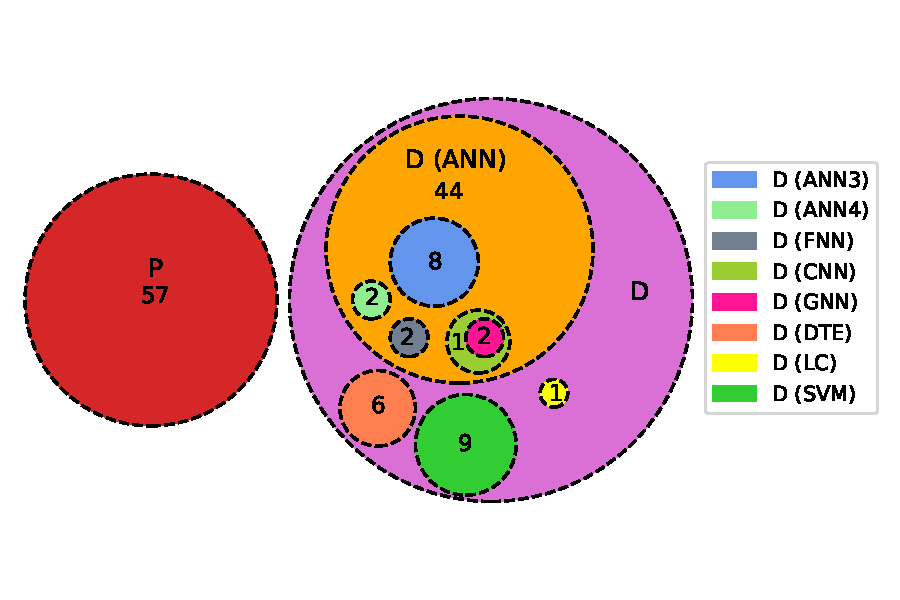
\includegraphics[width=.6\linewidth]{figures/ske-translucency}
    \caption[Venn diagram categorising SKE methods]{
        %
        Venn diagram categorising \gls{SKE} methods w.r.t.\ the \emph{translucency} of the algorithm: decompositional (D) or pedagogical (P).
        %
        For decompositional methods, we report the target predictor type: ANN<n> = artificial \gls{NN} (possibly having exactly <n> layers), CNN = convolutional \gls{NN}, GNN = graph \gls{NN}, FNN = fuzzy \gls{NN}, SVM = support vector machines, DTE = decision tree ensembles, LC = linear classifiers.
        %
        The image is taken from~\cite{DBLP:journals/csur/CiattoSAMO24} and it refers to 132 surveyed \gls{SKE} methods.
    }
    \label{fig:pie-ske-translucency}
\end{figure}
%
The sort of \gls{ML} predictors from which symbolic knowledge can be extracted is strongly related to the \emph{translucency} of the \gls{SKE} algorithms.
%
The translucency of a \gls{SKE} algorithm refers to its ability to access the internal structure of the predictor, such as its parameters, weights, and architecture.
%
So, in other words, the question of where to extract symbolic knowledge is related to the question of how \gls{SKE} algorithms work.
%
There are two ways for \gls{SKE} methods to deal with sub-symbolic predictors:
%
\begin{itemize}
    \item \textbf{Decompositional} $\rightarrow$ if the method needs to inspect -- even partially -- the internal structure of the predictor, such as its parameters, weights, and architecture;
    %
    \item \textbf{Pedagogical} $\rightarrow$ if the method does not need to inspect the internal structure of the predictor, but rather it can treat it as a black box and it relies on the input/output behavior of the predictor.
\end{itemize}

The different nature of decompositional \gls{SKE} methods is detailed in \Cref{fig:pie-ske-translucency}.
%
We observe that for what concern decompositional methods, the vast majority of them are designed to work with \gls{NN} of various types and different number of hidden layers.
%
Also \glspl{SVM} and \glspl{DTE} are targeted by some decompositional methods.
%
Around 43\% of the surveyed methods are pedagogical, meaning that these methods can work with virtually any type of sub-symbolic predictor, as long as it can be queried for input/output pairs.
%
Therefore, in general \gls{SKE} methods can be applied to any type of predictor, but for the decompositional ones, \glspl{NN} are definitely the most targeted type.


\subsection{How to extract}\label{subsec:how-to-extract}
%
The way \gls{SKE} methods extract symbolic knowledge highly depends on the translucency of the method itself.
%
Pedagogical methods treat the underlying predictor as an oracle to be queries for predictions the symbolic knowledge should mimic.
%
\note{TODO: add citations}
%
In most of these cases, the \gls{SKE} method exploits a \emph{surrogate} model, which is a simpler, more interpretable model that approximates the behavior of the original predictor.
%
This model can be used as the final output of the \gls{SKE} process if it is already in a symbolic or interpretable (e.g., a linear model) format, or it can be further processed to extract symbolic knowledge.
%
Decompositional methods, on the other hand, require access to the internal structure of the predictor and each method has its own way of extracting symbolic knowledge.
%
\note{TODO: does it make sense to talk about this here?}
%
Another important aspect of \gls{SKE} methods when it comes to how symbolic knowledge is extracted is the \emph{granularity} of the extraction.

\paragraph{Local explanations}\label{par:local-explanations}
%
\begin{figure}
    \centering
    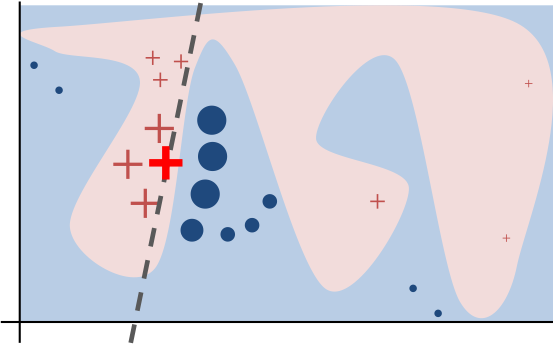
\includegraphics[width=.6\linewidth]{figures/local-explanation}
    \caption[Local explanations]{
        %
        Simple example to of how a local explanation can be provided for a specific input.
        %
        The sub-symbolic model's decision function $f$ is represented by the blue and pink background, which cannot be approximated well by a linear model.
        %
        The bold red cross is the instance being explained.
        %
        A \gls{SKE} method can sample inctances, get prediction using $f$, and weights them by the proximity to the instance being explained (the bigger the cross/circle, the closer to the instance).
        %
        The dashed line is the trained interpretable model that is locally faithful to the sub-symbolic model.
        %
        The image is taken from~\cite{DBLP:conf/kdd/Ribeiro0G16}.
    }
    \label{fig:local-explanations}
\end{figure}
%
When the interest in the extracted symbolic knowledge is focused on a specific input, i.e., we want to know why a predictor produced a particular outcome, the \gls{SKE} method is said to produce \emph{local explanations}.
%
A local explanation is symbolic knowledge that explains only the behavior of the predictor for a specific input.
%
The knowledge is not necessary encoded into logic rules, it can be provided for instance through \emph{feature importance} scores, which indicate the relevance of each input feature for the prediction~\cite{DBLP:conf/kdd/Ribeiro0G16}.
%
\Cref{fig:local-explanations} illustrates a simple example of how a local explanation can be provided for a specific input using a pedagogical \gls{SKE} method.


\paragraph{Global explanations}\label{par:global-explanations}
%
Conversely, when the interest is in understanding the overall behavior of the predictor, we say that the \gls{SKE} method produces \emph{global explanations}.
%
Global explanations aim to capture the general patterns and rules that govern the predictor's behavior across all inputs, rather than focusing on individual instances.
%
For example, this can be done by training a surrogate model -- if we want to use a pedagogical \gls{SKE} method -- using for instance the training set used to train the predictor.
%
However, instead of using the labels of the training set, the surrogate model is trained using the predictions of the original predictor.


\subsection[Limitations and challenges of SKE]{Limitations and challenges of \Gls{SKE}}\label{subsec:limitations-and-challenges-of-ske}
\note{TODO}
%%! Author = matteomagnini
%! Date = 05/03/25

%----------------------------------------------------------------------------------------
\chapter{Large Language Models}
\label{ch:llm}
\minitoc
%----------------------------------------------------------------------------------------

\section{Architectures}\label{sec:llm-architectures}

\subsection{Transformer}\label{subsec:transformer}

\subsection{Attention}\label{subsec:attention}

\section{Fine-tuning}\label{sec:llm-fine-tuning}

\section{\Glsentrylong{RAG}}\label{sec:rag}

\subsection{Embedding}\label{subsec:rag-embedding}

\subsection{Retrieval}\label{subsec:retrieval}

\section{Limitations and challenges}\label{sec:limitations-and-challenges}

\subsection{Resources}\label{subsec:resources}

\subsection{Data and privacy}\label{subsec:data-and-privacy}

\subsection{Hallucinations}\label{subsec:hallucinations}

\subsection{Stochastic parrot or something more?}\label{subsec:stochastic-parrot-or-something-more}
\printbibliography[title=References,heading=bibintoc]
\end{refsection}

%----------------------------------------------------------------------------------------
%-------------------------------------- PART II -----------------------------------------
%----------------------------------------------------------------------------------------

\part{Methods and Platform for \gls{SKI} \& \gls{SKE}}
\label{part:engineering-of-ski-ske}

\begin{refsection}
%! Author = matteomagnini
%! Date = 05/03/25

%----------------------------------------------------------------------------------------
\chapter{SKI: methods and contributions}
\label{ch:ski-methods-and-contributions}

\begin{flushright}
\begin{minipage}{0.5\textwidth}
    How to design and implement \emph{\gls{SKI} methods}?

    -- \textbf{\Cref{itm:rq0,itm:rq3}}
\end{minipage}
\end{flushright}

\mtcaddchapter
\minitoc
%----------------------------------------------------------------------------------------

In this chapter we present two main algorithmic contributions to the field of \gls{SKI}.
%
First, we provide the motivations behind the design and development of these contributions in \Cref{sec:ski-motivations}.
%
Second, we detail the contributions themselves in \Cref{sec:ski-contribution-kill,sec:ski-contribution-kins}, and we report the results of the empirical evaluation of these contributions.
%
Finally, we discuss the implications of these contributions and outline future directions in \Cref{sec:ski-discussion-and-future-direction}.


\section{Motivations}\label{sec:ski-motivations}
%
Aware by the limitations reported in \Cref{subsec:limitations-and-challenges-of-ski}, we wanted to develop novel \gls{SKI} methods that could be used in many different domains.
%
For this reason, these methods include all the elements described in \Cref{subsec:how-to-inject}.
%
In particular, a \emph{parser} is provided to convert symbolic knowledge into a format that can be injected into a neural network.
%
In this way, we are not bounded to a specific knowledge base nor to a specific domain.
%
The transformation of the parsed rules into a numeric interpretation is automatically performed by a \emph{fuzzification step}.
%
Finally, the sub-symbolic component is injected into a neural network, which is trained to learn the symbolic knowledge.
%
Another limitation that we wanted to address is the expressiveness of the symbolic knowledge that can be injected.
%
What we target in these two works is knowledge expressed in \emph{stratified Datalog with negation}.


\subsection{Stratified Datalog with negation}\label{subsec:ski-stratified-datalog-with-negation}
%
This logic is a variant of Datalog~\cite{DBLP:books/mc/18/MaierTKW18} with no recursion -- neither direct nor indirect -- yet supporting negated atoms.
%
We choose Datalog because of its expressiveness (strictly higher than propositional logic) and its acceptable limitations.
%
The lack of recursion, in particular, prevents issues when it comes to convert formulas into neural structures (which are \glspl{DAG}).
%
Since we rely on Datalog with negation, we allow atoms in the bodies od clauses to be negated.
%
Using the same notation as in \Cref{subsubsec:datalog}, in case the $i^{th}$ atom in the body of some clause is negated, we write $\neg b_{i}$.
%
There, each atom $h$, $b_{1}$, $b_{2}$, \dots{} may be a predicate of arbitrary arity.

An \(l\)-ary predicate \(p\) denotes a relation among \(l\) entities: \(p(t_1, \dots, t_l)\), where each \(t_i\) is a term, i.e., either a constant (denoted in \texttt{monospace}) representing a particular entity, or a logic variable (denoted by \textit{Capitalised Italic}) representing some unknown entity or value.
%
Well-known binary predicates – e.g., \(>\), \(<\), \(=\) – are admissible, too, and retain their usual semantics from arithmetic.
%
For the sake of readability, we may write these predicates in infix form—hence \(>(X, 1) \equiv X > 1\).

To support injection into a particular \gls{NN}, we further assume the input knowledge base defines one (and only one) outer relation -- say \texttt{output} or \texttt{class} -- involving as many variables as the input and output features the \gls{NN} has been trained upon.
%
That relation must be defined via one clause per output neuron.
%
Yet, each clause may contain other predicates in their bodies, in turn defined by one or more clauses.
%
In that case, since we rely on stratified Datalog, we require the input knowledge to not include any (directly or indirectly) recursive clause definition.

For example, for a 3-class classification task, any provided knowledge base should include a clause such as the following one:
%
\begin{align*}
    \texttt{class}(\bar{X}, y_1) &\leftarrow \texttt{p}_1(\bar{X}) \land \texttt{p}_2(\bar{X}) \\
    \texttt{p}_1(\bar{X}) &\leftarrow \dots \\
    \texttt{p}_2(\bar{X}) &\leftarrow \dots \\
    \texttt{class}(\bar{X}, y_2) &\leftarrow \texttt{p}'_1(\bar{X}) \land \texttt{p}'_2(\bar{X}) \\
    \texttt{p}'_1(\bar{X}) &\leftarrow \dots \\
    \texttt{p}'_2(\bar{X}) &\leftarrow \dots \\
    \texttt{class}(\bar{X}, y_3) &\leftarrow \texttt{p}''_1(\bar{X}) \land \texttt{p}''_2(\bar{X}) \\
    \texttt{p}''_1(\bar{X}) &\leftarrow \dots \\
    \texttt{p}''_2(\bar{X}) &\leftarrow \dots
\end{align*}
%
where \(\bar{X}\) is a tuple having as many variables as the neurons in the output layer, \(y_i\) is a constant denoting the \(i\)-th class, and \(\texttt{p}_1\), \(\texttt{p}_2\), \(\texttt{p}'_1\), \(\texttt{p}'_2\), \(\texttt{p}''_1\), \(\texttt{p}''_2\) are ancillary predicates defined via Horn clauses as well.


\section{Knowledge injection via lambda layer}\label{sec:ski-contribution-kill}
%
In this section we present the paper ``A view to a KILL: Knowledge Injection via Lambda Layer''~\cite{kill-woa2022}, presented at the 23rd Workshop ``From Objects to Agents'' (WOA 2022)~\footnote{\url{https://sites.google.com/view/woa2022/}}.
%
The paper introduces a novel \gls{SKI} method, called \gls{KILL}, which allow to inject symbolic knowledge in stratified Datalog with negation into \glspl{NN} of any shape.
%
\Gls{KILL} does not require the input formulas to be \emph{ground}, and it does not impose any constraint on the \gls{NN} undergoing injection.
%
The method acts directly at the backpropagation level, by increasing the penalty to be back-propagated whenever the \gls{NN} output is violating the knowledge to be injected.
%
For this reason, \gls{KILL} falls under the \emph{guided learning} strategy, as described in \Cref{subsec:how-to-inject}.


\subsection{$\Lambda$-layer}\label{subsec:lambda-layer}
%
\begin{figure}
    \centering
    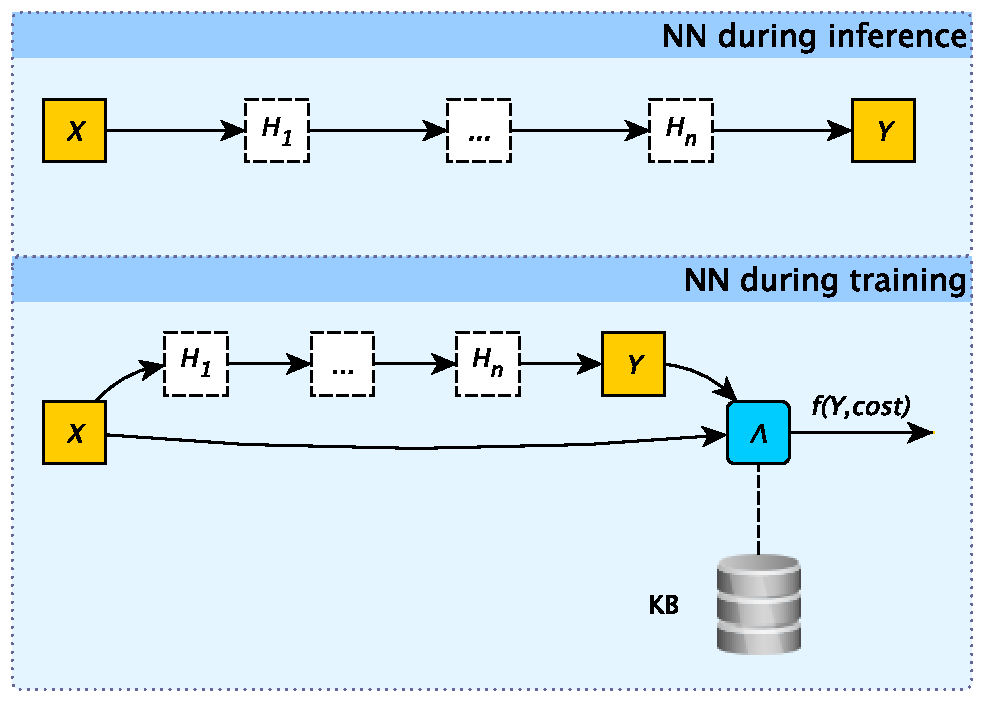
\includegraphics[width=0.8\linewidth]{figures/lambda-layer}
    \caption[General architecture of a NN with $\Lambda$-layer]{
        General architecture of a \gls{NN} with $n$ hidden layers, $X$ and $Y$ are respectively the input and output layers.
        %
        Before training, \gls{KILL} is applied to the predictor so that a new model constrained by the knowledge base (KB) is obtained.
        %
        The $\Lambda$-layer is added to the output layer, and then removed for the inference phase.
    }
    \label{fig:lambda-layer}
\end{figure}
%
The idea behind \gls{KILL} is to perform injection during training.
%
The injection is performed by appending one further layer -- the \emph{$\Lambda$-layer} -- at the output end of the \gls{NN}, and by training the overall network as usual (e.g., via gradient descent or similar).
%
The $\Lambda$-layer introduces an error whenever the prediction from the network's output layer violates the symbolic knowledge being injected.
%
This error influences the gradient descent or other optimization functions, discouraging violations of the symbolic knowledge.
%
In essence, the \gls{NN} learns inductively to avoid wrong predictions by penalizing violations during training.
%
To achieve this, the $\Lambda$-layer employs a custom activation function that modifies the output of the network's original output layer.
%
Additionally, the symbolic knowledge must be numerically interpreted, converting logical formulas into real-valued functions to compute error values.
%
Once the training phase is complete, the $\Lambda$-layer can be removed, leaving the original network architecture intact.


To elaborate on the $\Lambda$-layer, we consider a symbolic knowledge base, denoted as \(\mathcal{K}\), to be injected into a feedforward \gls{NN} of arbitrary depth, denoted as \(\mathcal{N}\).
%
Let \(\mathcal{N}\) have an input layer \(\mathbf{X}\) and an output layer \(\mathbf{Y}\), where \(\mathbf{Y}\) is assumed to be of shape \(n \times 1\).
%
This discussion applies to layers of any shape, including multidimensional ones.
%
No assumptions are made about the activation function of \(\mathbf{Y}\), the topology or nature of the hidden layers, or the shape of \(\mathbf{X}\).
%
The output of \(\mathbf{Y}\) is denoted as \(\mathbf{y} = [y_1, \dots, y_n]\), representing the network's prediction for a given input \(\mathbf{x}\).
%
The knowledge base \(\mathcal{K}\) consists of \(n\) rules, \(\mathcal{K} = \{\varphi_1, \dots, \varphi_n\}\), where each rule \(\varphi_i\) constrains the relationship between \(\mathbf{x}\) and \(y_i\).


To inject \(\mathcal{K}\), the $\Lambda$-layer is added to the network architecture, as illustrated in \Cref{fig:lambda-layer}.
%
This layer is densely connected to both \(\mathbf{X}\) and \(\mathbf{Y}\), and its activation function introduces a penalty on \(y_i\) whenever the corresponding rule \(\varphi_i\) is violated for an input-output pair \((\mathbf{x}, \mathbf{y})\).
%
The output of the $\Lambda$-layer, denoted as \(\boldsymbol{\lambda}\), is defined as:
%
\[
\boldsymbol{\lambda} = \mathbf{y} \times (1 + \mathbf{C}(\mathbf{x}, \mathbf{y}))
\]
%
where \(\mathbf{C}(\mathbf{x}, \mathbf{y})\) is a positive penalty vector representing the cost of modifying the network's output \(\mathbf{y}\).
%
The penalty vector \(\mathbf{C}(\mathbf{x}, \mathbf{y})\) is given by:
%
\[
\mathbf{C}(\mathbf{x}, \mathbf{y}) = [c_1(\mathbf{x}, y_1), \dots, c_i(\mathbf{x}, y_i), \dots, c_n(\mathbf{x}, y_n)]
\]
%
where \(c_i : \mathbf{X} \times \mathbf{Y} \to [0, 1]\) interprets the rule \(\varphi_i\) as a cost in the range \([0, 1]\) for the given values of \(\mathbf{x}\) and \(y_i\).
%
A penalty is applied to the \(i\)-th neuron of \(\mathbf{Y}\) whenever the corresponding rule \(\varphi_i\) is violated.
%
The penalty is higher when the violation is severe and approaches zero when the violation is minimal or absent.


\subsection{KILL fuzzifier}\label{subsec:kill-fuzzifier}
%
% !TeX spellcheck = en_GB
% !TeX root = ../phd-thesis.tex

\begin{table}
    \centering
    %
    \begin{tabular}{l|r||cl|r}
        \textbf{Formula} & \textbf{C. interpretation} & & \textbf{Formula} & \textbf{C. interpretation}
        \\
        \hline\hline
        $\llbracket\neg \phi\rrbracket$ & $\eta(1 - \llbracket\phi\rrbracket)$ & & $\llbracket\phi \le \psi\rrbracket$  & $\eta(\llbracket\phi\rrbracket - \llbracket\psi\rrbracket)$
        \\
        $\llbracket\phi  \wedge \psi\rrbracket$ &  $\eta(max(\llbracket\phi\rrbracket, \llbracket\psi\rrbracket))$ & & $\llbracket \pred{class}(\bar{X}, \const{y}_i) \leftarrow \psi \rrbracket$ & $\llbracket \psi \rrbracket^{*}$
        \\
        $\llbracket\phi  \vee \psi\rrbracket$ & $\eta(min(\llbracket\phi\rrbracket, \llbracket\psi\rrbracket))$ & & $\llbracket \text{expr}(\bar{X}) \rrbracket$ & $\text{expr}(\llbracket\bar{X}\rrbracket)$
        \\
        $\llbracket\phi = \psi\rrbracket$ & $\eta(|\llbracket\phi\rrbracket-\llbracket\psi\rrbracket|)$ & & $\llbracket \mathtt{true} \rrbracket$ & $0$
        \\
        $\llbracket\phi \ne \psi\rrbracket$ & $\llbracket \neg ( \phi = \psi )\rrbracket$ & & $\llbracket \mathtt{false} \rrbracket$ & $1$
        \\
        $\llbracket\phi > \psi\rrbracket$  & $\eta(0.5 - \llbracket\phi\rrbracket + \llbracket\psi\rrbracket) $ & & $\llbracket X \rrbracket$ & $x$
        \\
        $\llbracket\phi \ge \psi\rrbracket$ & $\eta(\llbracket\psi\rrbracket - \llbracket\phi\rrbracket)$ & & $\llbracket \const{k} \rrbracket$ & $k$
        \\
        $\llbracket\phi < \psi\rrbracket$  &  $\eta(0.5 + \llbracket\phi\rrbracket - \llbracket\psi\rrbracket)$ & & $\llbracket \pred{p}(\bar{X}) \rrbracket^{**}$ & $\llbracket \psi_1 \vee \ldots \vee \psi_k \rrbracket$
        
    \end{tabular}
    %
    \begin{center}\scriptsize
        $^{*}$ encodes the penalty for the $i^{th}$ neuron
        \\
        \smallskip
        $^{**}$ assuming predicate $p$ is defined by $k$ clauses of the form:
        \\
        $\pred{p}(\bar{X}) \leftarrow \psi_1,\ \ldots,\ \pred{p}(\bar{X}) \leftarrow \psi_k$
    \end{center}
    %
    \caption[KILL Fuzzifier: Logic Formulae Encoding]{
        Logic formulas' encoding into real-valued functions.
        %
        There, $X$ is a logic variable, while $x$ is the corresponding real-valued variable, whereas is $\bar{X}$ a tuple of logic variables.
        %
        Similarly, $\const{k}$ is a numeric constant, and $k$ is the corresponding real value, whereas $\const{k}_i$ is the constant denoting the $i^{th}$ class of a classification problem.
        %
        Finally, $\text{expr}(\bar{X})$ is an arithmetic expression involving the variables in $\bar{X}$.
    }
    %
    \label{tab:kill-logic-formulae}
    %
\end{table}
%
% !TeX spellcheck = en_GB
% !TeX root = ../phd-thesis.tex

\begin{figure*}[t]
    \centering
    \def\astscale{0.4}
    \begin{minipage}[c]{0.4\textwidth}
        \centering
        \begin{subfigure}{\linewidth}
            \centering
            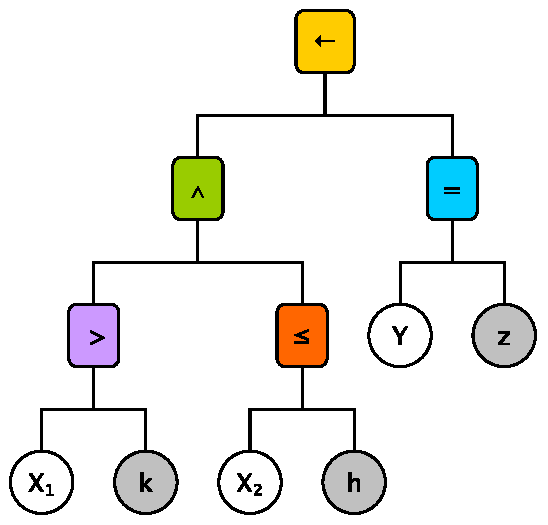
\includegraphics[scale=\astscale]{figures/ast-unencoded}
            \subcaption{AST of a logic formula}
            \label{fig:ast-kill-unencoded}
        \end{subfigure}
        \vspace{1.5ex}
        \tikz{\draw[->, thick] (0,0) -- (0,-0.4);}
        \vspace{2ex}
        \begin{subfigure}{\linewidth}
            \centering
            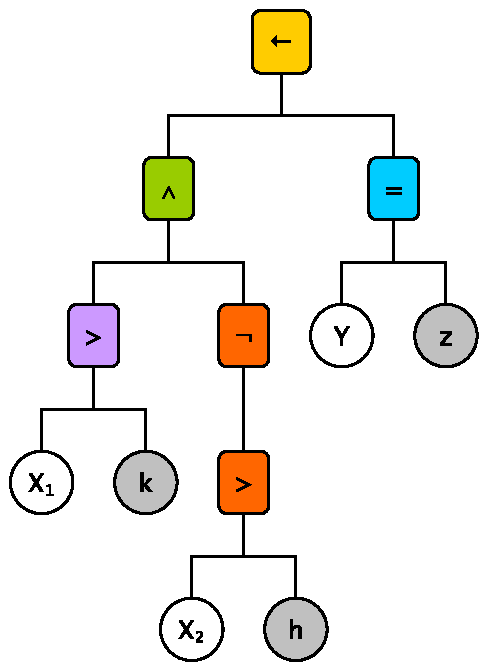
\includegraphics[scale=\astscale]{figures/ast-simplified}
            \subcaption{Simplified AST of a logic formula}
            \label{fig:ast-kill-simplified}
        \end{subfigure}
    \end{minipage}
    \hspace{0.5cm}
    \raisebox{-1cm}{\tikz{\draw[->, thick] (0,0) -- (0.7,0);}}
    \hspace{0.5cm}
    \begin{minipage}[c]{0.4\textwidth}
        \centering
        \begin{subfigure}{\linewidth}
            \centering
            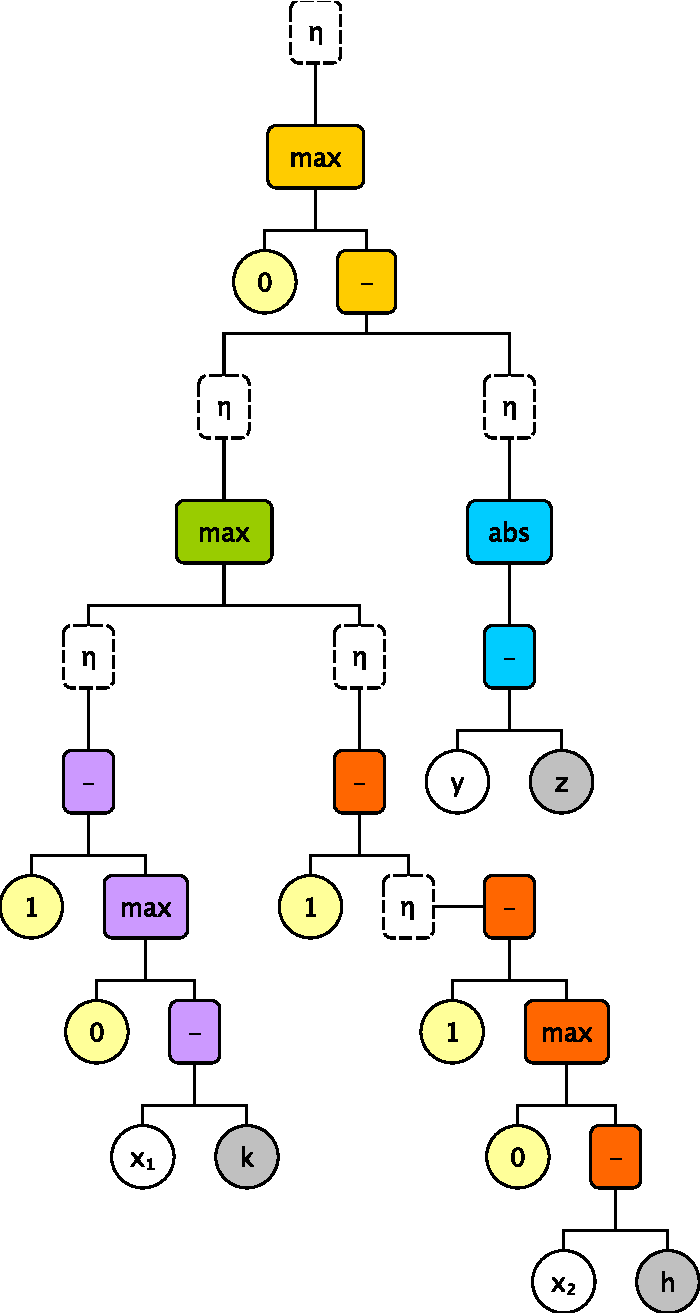
\includegraphics[scale=\astscale]{figures/ast-encoded}
            \subcaption{AST of the same formula, encoded as real-valued function}
            \label{fig:ast-kill-encoded}
        \end{subfigure}
    \end{minipage}
    \caption[KILL Encoding of logic formulas into real-valued functions]{
        %
        Example of the encoding process of logic formulas into real-valued functions.
        %
        Only \gls{AST} are depicted.
        %
        Boxes coloured in the same way represent the encoding of a given operator through each encoding step.
        %
        For instance, operator $<$ (red) is first converted into a negated $\geq$, and then into a combination of $max$ and subtractions.
    }
    \label{fig:ast-kill}
\end{figure*}

%
Before injecting symbolic knowledge into a neural network, each formula associated with an output neuron must be converted into a real-valued function to compute the cost of violating that formula.

This conversion relies on a multivalued interpretation of logic inspired by \L{}ukasiewicz's logic~\cite{DBLP:journals/jsyml/Hay63}.
%
Each formula is encoded using the \(\llbracket \cdot \rrbracket\) function, which maps logical formulas to real-valued functions.
%
These functions accept real vectors of size \(m + n\) as input and return scalars in \(\mathbb{R}\) as output.
%
The resulting scalars are clipped to the \([0, 1]\) range using the \(\eta : \mathbb{R} \to [0, 1]\) function, defined as:
%
\begin{equation}
    \label{eq:eta-function}
    \eta(x) =
    \begin{cases}
        0 & \text{if } x \leq 0, \\
        x & \text{if } 0 < x < 1, \\
        1 & \text{if } x \geq 1.
    \end{cases}
\end{equation}

The values obtained from \(\eta(x)\) represent penalties, as discussed in \Cref{subsec:lambda-layer}.
%
The penalty for the \(i^{\text{th}}\) neuron violating rule \(\varphi_i\) is expressed as \(c_i(\mathbf{x}, y_i) = \eta(\llbracket \varphi_i \rrbracket(\mathbf{x}, y_i))\).

The \(\llbracket \cdot \rrbracket\) encoding function is recursively defined in \Cref{tab:kill-logic-formulae}.
%
To compute the penalty \(c_i(\mathbf{x}, y_i)\) for the \(i^{\text{th}}\) neuron, \gls{KILL} identifies the Datalog rule of the form:
%
\begin{align*}
    \texttt{class}(\bar{X}, y_i) &\leftarrow \psi.
\end{align*}
%
The method focuses on the body \(\psi\) of the rule, ignoring its head, as the head specifies the expected output for the rule.
%
If \(\psi\) contains predicates \(p_1, p_2\), defined by one or more clauses in the knowledge base, these predicates are replaced by the disjunction of the bodies of all clauses defining them.
%
This process is repeated until \(\psi\) contains only binary expressions involving input variables, constants, arithmetic operators, and logical connectives.
%
Finally, operators and connectives are replaced by continuous functions, as detailed in \Cref{tab:kill-logic-formulae}.
%
The entire process produces a real-valued interpretation of the original formula, which \gls{KILL} uses to compute \(c_i(\mathbf{x}, y_i)\).

\Cref{fig:ast-kill} illustrates an example of the encoding process.
%
The example formula is:
%
\begin{align*}
    \texttt{class}(X_1, X_2, z) &\leftarrow (X_1 \geq k) \land (X_2 \geq h),
\end{align*}
%
where \(k\), \(h\), and \(z\) are numeric constants, \(X_1\) and \(X_2\) are input variables, and \(Y\) is an output variable.
%
\Cref{fig:ast-kill-unencoded} shows the \gls{AST} of this formula.
%
\Cref{fig:ast-kill-simplified} depicts the same \gls{AST} after replacing the \(\leq\) operator with a negated \(>\) operator.
%
Finally, \Cref{fig:ast-kill-encoded} shows the \gls{AST} of the encoded function.
%
A public implementation of \gls{KILL} is available as part of the \gls{PSyKI}~\cite{DBLP:conf/atal/MagniniCO22} library\footnote{\label{foot:psyki}\url{https://github.com/psykei/psyki-python}}.


\subsection{Validation}\label{subsec:kill-validation}
%
% !TeX spellcheck = en_GB
% !TeX root = ../phd-thesis.tex

\begin{table}[!t]
    \centering
    % \begin{adjustbox}{width=0.8\linewidth,center}
    \begin{tabular}{l|r|r|r|r}
        \textbf{Class} & \makecell{\textbf{Train.}\\\textbf{Instances}} & \makecell{\textbf{Train.}\\\textbf{Freq. (\%)}} & \makecell{\textbf{Test}\\\textbf{Instances}} & \makecell{\textbf{Test}\\\textbf{Freq. (\%)}}
        \\\hline\hline
        \text{high card} & 12,493 &  49.95 & 501,209 &  50.12
        \\
        \text{pair} & 10,599 & 42.38 & 422,498 & 42.25
        \\
        \text{two pairs} & 1,206 & 4.82 & 47,622 & 4.76
        \\
        \text{three of a kind} & 513 & 2.05 & 21,121 & 2.11
        \\
        \text{straight} & 93 & 0.37 & 3,885 & 0.39
        \\
        \text{flush} & 54 & 0.22 & 1,996 & 0.2
        \\
        \text{full house} & 36 & 0.14 & 1,424 & 0.14
        \\
        \text{four of a kind} & 6 & 0.024 & 230 & 0.023
        \\
        \text{straight flush} & 5 & 0.02 & 12 & 0.001
        \\
        \text{royal flush} & 5 &  0.02 & 3 & \scinum{3}{-4}
        \\
        \hline
        \textbf{Total} & 25,010 & 100 & 1,000,000 & 100
    \end{tabular}
    % \end{adjustbox}
    \caption[PHDS statistics per class]{
        \Gls{PHDS} statistics per class.
        %
        The dataset is heavily imbalanced, with the \emph{high card} class being the most frequent.
        %
        Considering together the two most frequent classes, \emph{high card} and \emph{pair}, they account for over 92\% of the training instances.
    }
    \label{tab:phds-dataset}
\end{table}
%
The method has been validated on the \glsentrylong{PHDS} (\glsentryshort{PHDS})~\cite{poker_hand_158}, a dataset for poker hand classification.
%
To ensure reproducibility, the code used for our experiments is publicly available\footnote{\url{https://github.com/MatteoMagnini/kill-experiments-woa-2022}}.
%
The task consists in a multiclass classification problem on a finite -- yet very large -- discrete domain.
%
Classes are overlapped and heavily imbalanced, but exact classification rules can be written in logic formulas.
%
\Gls{PHDS} has $1,025,010$ records\footnote{the size of the input space is the amount 5-permutations of 52 cards, i.e., $\frac{52!}{(52 - 5)!}$}, each with $10$ features, and $1$ output class.
%
Each record represents a poker hand of $5$ cards, each card is identified by two features: a rank and a suit.
%
Suit is a categorical feature (e.g., \texttt{spades}, \texttt{hearts}, \texttt{diamonds}, \texttt{clubs}), while rank is a numeric feature (e.g., $1$ for Ace, $2$ for Two, \dots, $13$ for King).
%
Each hand can be classified as one of $10$ different classes denoting the poker hand type (e.g., \texttt{high card}, \texttt{pair}, \texttt{two pairs}, \texttt{three of a kind}, etc.).
%
\Cref{tab:phds-dataset} reports the statistics of the dataset per class for both training and test sets.


\paragraph{\Gls{PHDS} logic rules}\label{par:phds-logic-rules}
%
% !TeX spellcheck = en_GB
% !TeX root = ../phd-thesis.tex

\begin{table}
    \centering
    \begin{adjustbox}{width=\linewidth, center}
        \begin{tabular}{c|p{1.385\linewidth}}
            \textbf{Class} & \textbf{Logic Formulation}
            \\\hline\hline
            Pair & $\begin{array}{l}
                \pred{class}(R_1, \ldots, S_5, \const{pair}) \leftarrow \pred{pair}(R_1, \ldots, S_5)
                \\
                \pred{pair}(R_1, \ldots, S_5) \leftarrow R_1 = R_2
                \\
                \pred{pair}(R_1, \ldots, S_5) \leftarrow R_1 = R_3
                \\
                \pred{pair}(R_1, \ldots, S_5) \leftarrow R_1 = R_4
                \\
                \pred{pair}(R_1, \ldots, S_5) \leftarrow R_1 = R_5
                \\
                \pred{pair}(R_1, \ldots, S_5) \leftarrow R_2 = R_3
                \\
                \pred{pair}(R_1, \ldots, S_5) \leftarrow R_2 = R_4
                \\
                \pred{pair}(R_1, \ldots, S_5) \leftarrow R_2 = R_5
                \\
                \pred{pair}(R_1, \ldots, S_5) \leftarrow R_3 = R_4
                \\
                \pred{pair}(R_1, \ldots, S_5) \leftarrow R_3 = R_5
                \\
                \pred{pair}(R_1, \ldots, S_5) \leftarrow R_4 = R_5
            \end{array}$
            \\\hdashline
            Two Pairs & $\begin{array}{l}
                \pred{class}(R_1, \ldots, S_5, \const{two}) \leftarrow \pred{two}(R_1, \ldots, S_5)
                \\
                \pred{two}(R_1, \ldots, S_5) \leftarrow R_1 = R_2 \wedge R_3 = R_4
                \\
                \pred{two}(R_1, \ldots, S_5) \leftarrow R_1 = R_3 \wedge R_2 = R_4
                \\
                \pred{two}(R_1, \ldots, S_5) \leftarrow R_1 = R_4 \wedge R_2 = R_3
                \\
                \pred{two}(R_1, \ldots, S_5) \leftarrow R_1 = R_2 \wedge R_3 = R_5
                \\
                \pred{two}(R_1, \ldots, S_5) \leftarrow R_1 = R_3 \wedge R_3 = R_5
                \\
                \pred{two}(R_1, \ldots, S_5) \leftarrow R_1 = R_5 \wedge R_2 = R_3
                \\
                \pred{two}(R_1, \ldots, S_5) \leftarrow R_1 = R_2 \wedge R_4 = R_5
                \\
                \pred{two}(R_1, \ldots, S_5) \leftarrow R_1 = R_4 \wedge R_2 = R_5
                \\
                \pred{two}(R_1, \ldots, S_5) \leftarrow R_1 = R_5 \wedge R_2 = R_4
                \\
                \pred{two}(R_1, \ldots, S_5) \leftarrow R_1 = R_3 \wedge R_4 = R_5
                \\
                \pred{two}(R_1, \ldots, S_5) \leftarrow R_1 = R_4 \wedge R_3 = R_5
                \\
                \pred{two}(R_1, \ldots, S_5) \leftarrow R_1 = R_5 \wedge R_3 = R_4
                \\
                \pred{two}(R_1, \ldots, S_5) \leftarrow R_2 = R_3 \wedge R_4 = R_5
                \\
                \pred{two}(R_1, \ldots, S_5) \leftarrow R_2 = R_4 \wedge R_3 = R_5
                \\
                \pred{two}(R_1, \ldots, S_5) \leftarrow R_2 = R_5 \wedge R_3 = R_4
            \end{array}$
            \\\hdashline
            Three of a Kind & $\begin{array}{l}
                \pred{class}(R_1, \ldots, S_5, \const{three}) \leftarrow \pred{three}(R_1, \ldots, S_5)
                \\
                \pred{three}(R_1, \ldots, S_5) \leftarrow R_1 = R_2 \wedge R_1 = R_3
                \\
                \pred{three}(R_1, \ldots, S_5) \leftarrow R_1 = R_2 \wedge R_1 = R_4
                \\
                \pred{three}(R_1, \ldots, S_5) \leftarrow R_1 = R_2 \wedge R_1 = R_5
                \\
                \pred{three}(R_1, \ldots, S_5) \leftarrow R_1 = R_3 \wedge R_1 = R_4
                \\
                \pred{three}(R_1, \ldots, S_5) \leftarrow R_1 = R_3 \wedge R_1 = R_5
                \\
                \pred{three}(R_1, \ldots, S_5) \leftarrow R_1 = R_4 \wedge R_1 = R_5
                \\
                \pred{three}(R_1, \ldots, S_5) \leftarrow R_2 = R_3 \wedge R_2 = R_4
                \\
                \pred{three}(R_1, \ldots, S_5) \leftarrow R_2 = R_3 \wedge R_2 = R_5
                \\
                \pred{three}(R_1, \ldots, S_5) \leftarrow R_2 = R_4 \wedge R_2 = R_5
                \\
                \pred{three}(R_1, \ldots, S_5) \leftarrow R_3 = R_4 \wedge R_3 = R_5
            \end{array}$
            \\\hdashline
            Straight & $\begin{array}{l}
                \pred{class}(R_1, \ldots, S_5, \const{straight}) \leftarrow \pred{royal}(R_1, \ldots, S_5)
                \\
                \pred{class}(R_1, \ldots, S_5, \const{straight}) \leftarrow \pred{straight}(R_1, \ldots, S_5)
                \\
                \pred{straight}(R_1, \ldots, S_5) \leftarrow (R_1 + R_2 + R_3 + R_4 + R_5) = (5 * \text{min}(R_1, \ldots, R_5) + 10) \wedge \neg \pred{pair}(R_1, \ldots, S_5)
                \\
                \pred{royal}(R_1, \ldots, S_5) \leftarrow \text{min}(R_1, \ldots, R_5) = 1 \wedge (R_1 + R_2 + R_3 + R_4 + R_5 = 47) \wedge \neg \pred{pair}(R_1, \ldots, S_5)
                \\
            \end{array}$
            \\\hdashline
            Flush & $\begin{array}{l}
                \pred{class}(R_1, \ldots, S_5, \const{flush}) \leftarrow \pred{flush}(R_1, \ldots, S_5)
                \\
                \pred{flush}(R_1, \ldots, S_5) \leftarrow S_1 = S_2 \wedge S_1 = S_3 \wedge S_1 = S_4 \wedge S_1 = S_5
            \end{array}$
            \\\hdashline
            Four of a Kind & $\begin{array}{l}
                \pred{class}(R_1, \ldots, S_5, \const{four}) \leftarrow \pred{four}(R_1, \ldots, S_5)
                \\
                \pred{four}(R_1, \ldots, S_5) \leftarrow R_1 = R_2 \wedge R_1 = R_3 \wedge R_1 = R_4
                \\
                \pred{four}(R_1, \ldots, S_5) \leftarrow R_1 = R_2 \wedge R_1 = R_3 \wedge R_1= R_5
                \\
                \pred{four}(R_1, \ldots, S_5) \leftarrow R_1 = R_2 \wedge R_1 = R_4 \wedge R_1 = R_5
                \\
                \pred{four}(R_1, \ldots, S_5) \leftarrow R_1 = R_3 \wedge R_1 = R_4 \wedge R_1 = R_5
                \\
                \pred{four}(R_1, \ldots, S_5) \leftarrow R_2 = R_3 \wedge R_2 = R_4 \wedge R_2 = R_5
            \end{array}$
            \\\hdashline
            Full House & $\begin{array}{l}
                \pred{class}(R_1, \ldots, S_5, \const{full}) \leftarrow three(S_1,\dots,R_5) \wedge two(S_1,\dots,R_5) \wedge \neg four(S_1,\dots,R_5)
            \end{array}$
            \\\hdashline
            Straight Flush & $\begin{array}{l}
                \pred{class}(R_1, \ldots, S_5, \const{straight\_flush}) \leftarrow \pred{straight}(R_1, \ldots, S_5) \wedge \pred{flush}(R_1, \ldots, S_5)
                \\
                 \pred{class}(R_1, \ldots, S_5, \const{straight\_flush}) \leftarrow \pred{royal}(R_1, \ldots, S_5) \wedge \pred{flush}(R_1, \ldots, S_5)
            \end{array}$
            \\\hdashline
            Royal Flush & $\begin{array}{l}
                \pred{class}(R_1, \ldots, S_5, \const{royal}) \leftarrow \pred{royal}(R_1, \ldots, S_5) \wedge \pred{flush}(R_1, \ldots, S_5)
            \end{array}$
            \\\hdashline
            High Card & $\begin{array}{l}
                \pred{class}(R_1, \ldots, S_5, \const{nothing}) \leftarrow \neg \pred{pair}(R_1, \ldots, S_5) \wedge \neg \pred{flush}(R_1, \ldots, S_5) \wedge \neg \pred{straight}(R_1, \ldots, S_5) \wedge \neg \pred{royal}(R_1, \ldots, S_5)
            \end{array}$
        \end{tabular}
    \end{adjustbox}
    \caption{
        Stritified datalog with negation formulas describing poker hands.
        %
        For the sake of readability variables in the head of formulas and in the arguments of predicates are abbreviated.
    }
    \label{tab:phds-logic-rules}
\end{table}
%
We define a \emph{class} rule for each class, encoding the correct way of classifying a poker hand.
%
For instance, let $\{R_{1}, S_{1}, \dots, R_{5}, S_{5}\}$ be the logic variables representing a poker hand (i.e., $R$ for rank and $S$ for suit), then for class \texttt{flush} we have:
%
\begin{equation}\label{eq:flush-class}
     \begin{array}{rcl}
        \pred{class}(R_1, S_1, \ldots, R_5, S_5, \const{flush}) & \leftarrow & \pred{flush}(R_1, S_1, \ldots, R_5, S_5)
        \\
        \pred{flush}(R_1, S_1, \ldots, R_5, S_5) & \leftarrow & S_1 = S_2 \wedge S_1 = S_3 \wedge S_1 = S_4 \wedge S_1 = S_5
    \end{array}
\end{equation}
%
All other rules have the same structure as \Cref{eq:flush-class}: the left-hand side declares the expected class, while the right-hand side describes the necessary conditions for that class—possibly, via some ancillary predicates such as \emph{flush}.
%
\Cref{tab:phds-logic-rules} provides an overview of all the rules we rely upon in our experiments.


\paragraph{Methodology}\label{par:phds-methodology}
%
We adopt the same data partitioning strategy proposed by the dataset authors~\cite{poker_hand_158}.
%
Specifically, the training set consists of $25,010$ samples, while the test set includes $1,000,000$ samples.
%
This unusual ratio between training and test set sizes makes the task more challenging but ensures more reliable results.

For all experiments, we use a fully connected \gls{NN} with three layers.
%
The first two layers consist of $128$ neurons each, while the output layer has $10$ neurons, corresponding to the number of classes.
%
The activation function for the first two layers is \gls{ReLU}, whereas the output layer uses softmax.
%
The network is trained using categorical cross-entropy as the loss function.

We set the batch size to $32$ and train the network for up to $100$ epochs.
%
To evaluate the network's performance, we rely on metrics such as accuracy, macro-F1, and weighted-F1 scores.
%
After training, the \(\Lambda\)-layer is removed, and the resulting \gls{NN} is used for inference.

To prevent overfitting, we employ three stopping criteria during training.
%
First, for 99\% of the training examples, the activation of every output unit must be within 0.25 of the correct value.
%
Second, training stops after 100 epochs.
%
Third, the predictor must achieve at least 90\% accuracy on the training examples but show no improvement in classification performance for five consecutive epochs.
%
These criteria are inspired by previous work~\cite{DBLP:conf/aaai/TowellSN90}.
%
Finally, we conduct 30 runs for each configuration to obtain a statistically significant population for comparisons.


\paragraph{Results and discussion}\label{par:phds-results}
%
% !TeX spellcheck = en_GB
% !TeX root = ../phd-thesis.tex

\begin{table}
    \centering
     \begin{adjustbox}{width=\linewidth,center}
         \begin{tabular}{l|rr||l|rr}
             \textbf{Metric} & \textbf{Uneducated} & \textbf{Educated} & \textbf{Metric} & \textbf{Uneducated} & \textbf{Educated}
             \\
             \hline\hline
             \textbf{Accuracy} & 0.962 & 0.978 & \textbf{Acc. Straight} & 0.415 & 0.509
             \\
             \textbf{Macro-F1} & 0.512 & 0.538 & \textbf{Acc. Flush} & 0.002 & 0.002
             \\
             \textbf{Weighted-F1} & 0.96 & 0.977 & \textbf{Acc. Full} & 0.628 & 0.69
             \\
             \textbf{Acc. High Card} & 0.977 & 0.989 & \textbf{Acc. Four} & 0.186 & 0.19
             \\
             \textbf{Acc. Pair} & 0.968 & 0.985 & \textbf{Acc. Straight F.} & 0.003 & 0
             \\
             \textbf{Acc. Two Pairs} & 0.867 & 0.914 & \textbf{Acc. Royal F.} & 0 & 0
             \\
             \textbf{Acc. Three} & 0.913 & 0.922 & & &
        \end{tabular}
     \end{adjustbox}
    \caption{
        Test set accuracy, macro-F1 and weighted-F1 on all classes and single mean class accuracies.
        %
        All measures represent the mean over the experiment population (30).
        %
        The Wilcoxon signed-rank test shows that for the accuracy, macro-F1 and weighted-F1 metrics the educated model is significantly better than the uneducated one ($p < 0.05$).
        %
        Also, the educated model is significantly better than the uneducated one for the single mean class accuracies, except for \emph{high card}, \emph{pair} and \emph{straight} classes.
    }
    \label{tab:phds-kill-results}
\end{table}
%
\begin{figure}
    \centering
    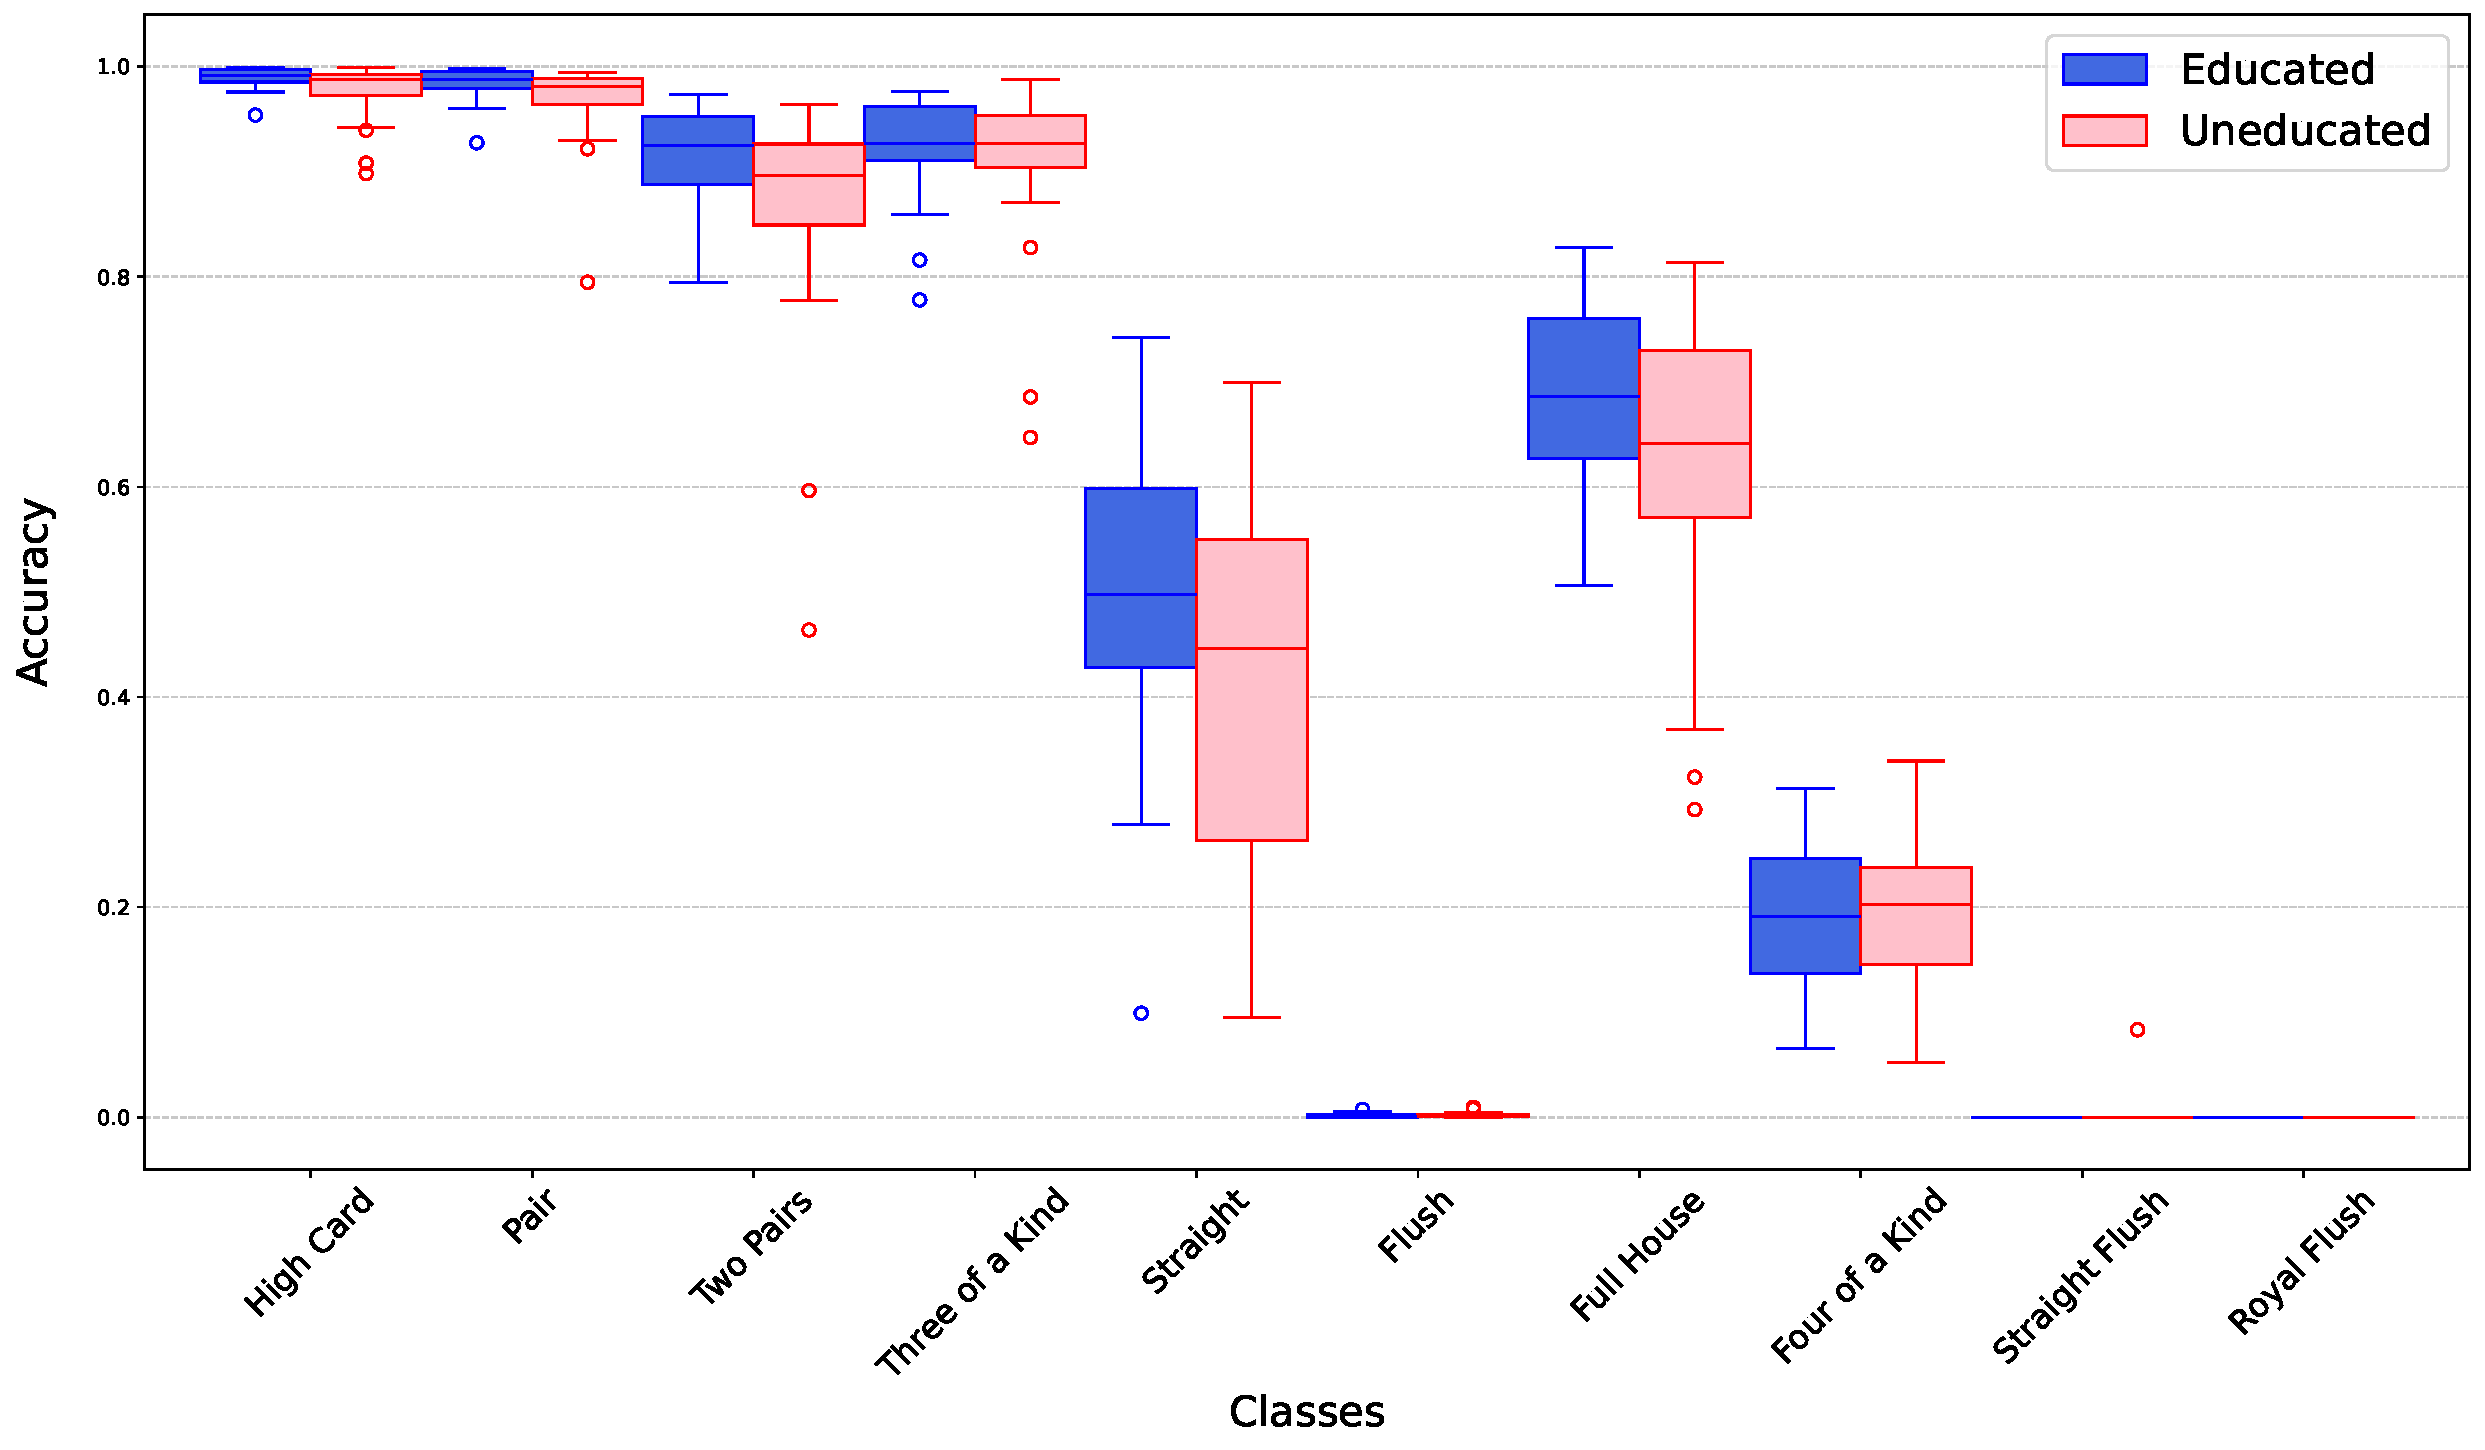
\includegraphics[width=\linewidth]{figures/phds-kill-results}
    \caption[PHDS KILL results]{
        Per class results of the experiments on the \gls{PHDS} dataset using \gls{KILL}.
        %
        The \gls{KILL} method outperforms the uneducated \gls{NN} in the prediction of almost all classes.
        %
        For all class prediction, the Wilcoxon signed-rank test has been applied to compare the two configurations.
        %
        With a p-value threshold of $0.05$, we reject the null hypothesis in the case of \emph{high card}, \emph{pair}, and \emph{straight} classes.
    }
    \label{fig:phds-kill-results}
\end{figure}
%
We define two different configurations for experiments:
%
\begin{inlinelist}
    %
    \item ``uneducated'', where we use the \gls{NN} described in \Cref{par:phds-methodology},
    %
    \item ``educated'', where we apply \gls{KILL} on the same network architecture.
    %
\end{inlinelist}
%
For both configurations we use the same hyperparameters and perform $30$ runs.
%
Results are reported in \Cref{tab:phds-kill-results} and in \Cref{fig:phds-kill-results}.
%
In general, experiments show that both predictors are very good at classifying frequent classes such as \emph{high card} and \emph{pair}.
%
Also for less frequent classes, \emph{two pairs} and \emph{three of a kind}, accuracy is still high.
%
The remaining six classes represent the $0.8\%$ of the training set and therefore much more difficult to correctly predict.
%
For \emph{full house} and \emph{straight}, accuracy has middle values, while for the remaining classes accuracy is pretty close to $0$.
%
All of this is quite expected due to the strong imbalance in the distribution of classes.
%
The only remarkable fact is that accuracy is extremely low for class \emph{flush} even if less frequent classes such as \emph{full house} and \emph{four of a kind} have higher accuracy.
%
We hypothesise that this happens because the vast majority of data consists in classes which depend only on the values of rank and therefore the network tends to consider it much more.
%
Indeed, only \emph{flush}, \emph{straight flush} and \emph{royal flush} (about the $0.26\%$ of the training set) depend on the values of suit.
%
Concerning the comparison between the \emph{uneducated} predictor -- with no additional knowledge -- and the \emph{educated} predictor -- obtained by applying KILL algorithm -- results show that the latter has higher performances with statistic significance.
%
The Wilcoxon signed-rank test~\cite{wilcoxon1945} has been applied to compare the two configurations on all the metrics reported in \Cref{tab:phds-kill-results}.
%
In particular, because of the imbalanced nature of the dataset, the test on macro-F1 and weighted-F1 metrics is more reliable than the test on accuracy.
%
The test shows that the \emph{educated} predictor is significantly better than the \emph{uneducated} one for the overall accuracy, macro-F1 and weighted-F1 metrics (with $p < 0.05$).
%
Also, the \emph{educated} predictor is significantly better than the \emph{uneducated} one for the single mean class accuracies, except for \emph{high card}, \emph{pair} and \emph{straight} classes.


\section{Knowledge injection via network structuring}\label{sec:ski-contribution-kins}
%
In this section we present the paper ``KINS: Knowledge Injection via Network Structuring''~\cite{kins-cilc2022}, presented at the 37th Italian Conference on Computational Logic (CILC 2022)~\footnote{\url{http://cilc2022.apice.unibo.it/}}.
%
The paper introduces a novel \gls{SKI} methods, named \gls{KINS}, which similarly to \gls{KILL} allows to inject symbolic knowledge in stratified Datalog with negation into \glspl{NN} of any shape.
%
Differently from \gls{KILL}, \gls{KINS} does not act at the backpropagation level, but it modifies the structure of the \gls{NN} to inject symbolic knowledge.
%
Hence, \gls{KINS} falls under the \emph{structuring} strategy, as described in \Cref{subsec:how-to-inject}.


\subsection{KINS architecture}\label{subsec:kins-architecture}
%
\begin{figure}
    \centering
    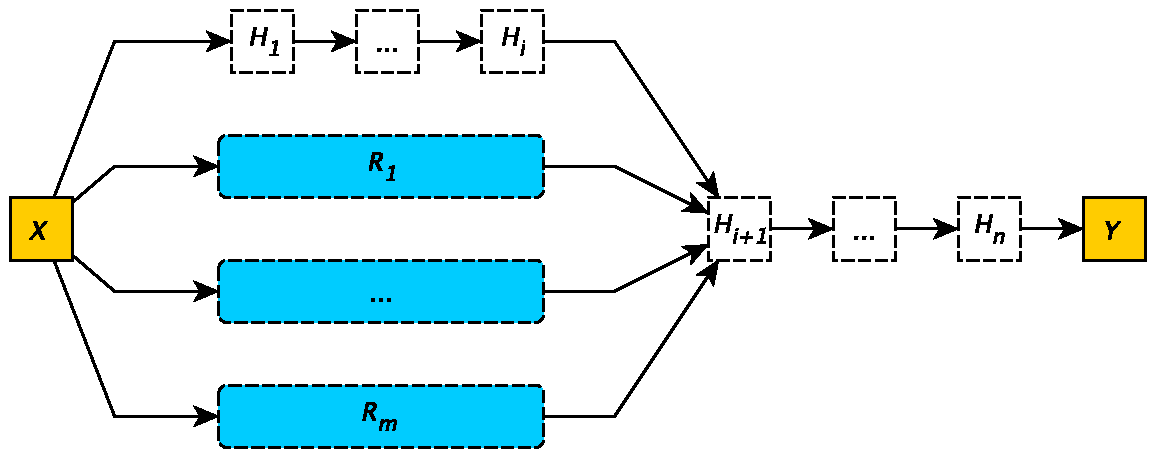
\includegraphics[width=\textwidth]{figures/kins-network-architecture}
    \caption[General architecture of a NN with KINS modules]{
        %
        General architecture of a \gls{NN} with $m$ modules injected, $X$ and $Y$ are respectively the input and output layers.
        %
        Each module is a subnetwork that evaluates a logic formula under a continuous interpretation.
        %
        The modules can be injected at any layer $H_i$ or at the output layer $Y$.
    }
    \label{fig:kins-network-architecture}
\end{figure}
%
A \gls{NN} architecture can be extended with additional neural \emph{modules} designed to reflect and mimic symbolic knowledge provided by designers.
%
Each module is a subnetwork that shares the same input layer as the original network and outputs a value representing the evaluation of a logic formula under a continuous interpretation.
%
The primary purpose of these modules is twofold:
\begin{inlinelist}
    %
    \item to evaluate a specific logic formula against the current input, and
    %
    \item to compute the degree of truth of that formula, expressed as a value in the range \([0, 1]\), which complements the network's output.
    %
\end{inlinelist}
%
During the feed-forward phase, variables in the formulas are dynamically grounded with respect to the current input.
%
This dynamic grounding allows non-ground formulas to be directly exploited for \gls{SKI}, eliminating the need for prior groundisation steps, which may be infeasible for complex domains.
%
It is important to note that the provided formulas are not required to cover all possible scenarios.
%
For instance, in classification problems, rules may only cover a subset of all possible classes.

\Cref{fig:kins-network-architecture} illustrates the general architecture of a \gls{NN} after the injection of \(m\) modules, represented as blue rectangles.
%
Each module corresponds to one of the \(m\) rules to be injected.
%
Modules can be arbitrarily complex subnetworks that share the same input and final outputs with the original \gls{NN}.
%
White boxes represent arbitrary hidden layers \(H_1, \dots, H_n\) of the original \gls{NN}, while \(X\) and \(Y\) denote the input and output layers, respectively.
%
Knowledge injection can be performed at any hidden layer \(H_i\) or at the output layer \(Y\).
%
For example, in networks that first extract features from the input (e.g., convolutional \glspl{NN}) and then perform classification, knowledge can be injected between these two phases.
%
The injection procedure involves three main steps.
%
First, formulas are encoded into real-valued functions, as described in \Cref{subsec:kill-fuzzifier}.
%
Second, a neural module is constructed to approximate each real-valued function, following the strategy outlined in \Cref{subsec:kill-fuzzifier}.
%
Finally, the module is added to the original \gls{NN}, as depicted in \Cref{fig:kins-network-architecture}.
%
The inner synapses of the modules can be either immutable, meaning their weights and biases remain fixed during training, or mutable, meaning their weights are trainable.
%
All other synapses, including those within hidden layers \(H_1, \dots, H_i\), as well as the ingoing synapses of layer \(H_{i+1}\) and subsequent layers, remain trainable.
%
This design allows the \gls{NN} to leverage both prior knowledge and information gathered from data during training.
%
The synapses connecting each module and the final hidden layer to the output layer are also trainable.
%
This enables the \gls{NN} to adjust the relative importance of the injected knowledge during training.
%
The rationale is that logic rules may not hold universally across all patterns in a given domain but may generally be true with a certain degree of confidence.

\gls{KINS} does not impose constraints on the network architecture, such as the number of layers, number of neurons, types of activation functions, or initialization status (e.g., random weights or partially trained).
%
It can be applied to both untrained and partially trained networks.
%
However, it requires the network to have an input and output layer and to be trainable via gradient descent or similar algorithms.
%
Additionally, symbolic knowledge must be expressed using one or more formulas in Datalog form, and logic statements about the network's input or output features must be encoded.


\subsection{KINS fuzzifier}\label{subsec:kins-fuzzifier}
%
% !TeX spellcheck = en_GB
% !TeX root = ../phd-thesis.tex

\begin{table}
    \centering
    \begin{tabular}{l|r||cl|r}
        \textbf{Formula} & \textbf{C. interpretation} & & \textbf{Formula} & \textbf{C. interpretation}
        \\
        \hline\hline
        $\llbracket\neg \phi\rrbracket$ & $\eta(1 - \llbracket\phi\rrbracket)$ & & $\llbracket\phi \le \psi\rrbracket$  & $\eta(1 + \llbracket \psi \rrbracket - \llbracket \phi \rrbracket)$  % Negation % Less equal
        \\
        $\llbracket\phi  \wedge \psi\rrbracket$ &  $\eta(min(\llbracket\phi\rrbracket, \llbracket\psi\rrbracket))$ & &  $\llbracket \pred{class}(\bar{X}, \const{y}_i) \leftarrow \psi \rrbracket$ & $\llbracket \psi \rrbracket^{*}$ % Conjunction % Class
        \\
        $\llbracket\phi  \vee \psi\rrbracket$ & $\eta(max(\llbracket\phi\rrbracket, \llbracket\psi\rrbracket))$ & & $\llbracket \text{expr}(\bar{X}) \rrbracket$ & $\text{expr}(\llbracket\bar{X}\rrbracket)$ % Disjunction
        \\
        $\llbracket\phi = \psi\rrbracket$ & $\eta(\llbracket\neg( \phi \ne \psi )\rrbracket )$ & &$\llbracket \mathtt{true} \rrbracket$ & $1$ % Equal
        \\
        $\llbracket\phi \ne \psi\rrbracket$ & $\eta(|\llbracket\phi\rrbracket-\llbracket\psi\rrbracket|)$ & & $\llbracket \mathtt{false} \rrbracket$ & $0$ % Not Equal
        \\
        $\llbracket\phi > \psi\rrbracket$ & $\eta(max(0, \frac{1}{2} + \llbracket\phi\rrbracket - \llbracket\psi\rrbracket))$ & & $\llbracket X \rrbracket$ & $x$ % Greater
        \\
        $\llbracket\phi \ge \psi\rrbracket$  & $\eta(1 + \llbracket \phi \rrbracket - \llbracket \psi \rrbracket)$ & & $\llbracket \const{k} \rrbracket$ & $k$ % Greater Equal
        \\
        $\llbracket\phi < \psi\rrbracket$  &  $\eta(max(0, \frac{1}{2} + \llbracket\psi\rrbracket - \llbracket\phi\rrbracket))$ & & $\llbracket \pred{p}(\bar{X}) \rrbracket^{**}$ & $\llbracket \psi_1 \vee \ldots \vee \psi_k \rrbracket$ % Less 
    \end{tabular}
    \begin{center}\scriptsize
        $^{*}$ encodes the value for the $i^{th}$ output
        \\
        \smallskip
        $^{**}$ assuming $p$ is defined by $k$ clauses of the form:
        \\
        $\pred{p}(\bar{X}) \leftarrow \psi_1,\ \ldots,\ \pred{p}(\bar{X}) \leftarrow \psi_k$
    \end{center}
    \caption{
        Logic formulas' encoding into real-valued functions.
        %
        There, $X$ is a logic variable, while $x$ is the corresponding real-valued variable, whereas is $\bar{X}$ a tuple of logic variables.
        %
        Similarly, $\const{k}$ is a numeric constant, and $k$ is the corresponding real value, whereas $\const{k}_i$ is the constant denoting the $i^{th}$ class of a classification problem.
        %
        Finally, $\text{expr}(\bar{X})$ is an arithmetic expression involving the variables in $\bar{X}$.
        %
        The $\eta$ function is a scaling function described in \Cref{eq:eta-function}.
    }
    \label{tab:kins-logic-formulae}
\end{table}


%
To inject symbolic knowledge into a neural network, each formula associated with an output neuron must first be converted into a real-valued function to compute the degree of truth of that formula.
%
This conversion relies on a multivalued interpretation of logic -- inspired by \L{}ukasiewicz's logic~\cite{DBLP:journals/jsyml/Hay63} -- similarly to the one used for \gls{KILL}.
%
Differently from \gls{KILL}, the fuzzification function is not used to compute a penalty, but rather to compute the degree of truth of the formula.
%
For this reason, $\mathtt{true}$ and $\mathtt{false}$ are interpreted as $1$ and $0$, respectively, rather than as $0$ and $1$.
%
While \Cref{tab:kins-logic-formulae} describes the mapping between formulas and their fuzzy interpretation, we now discuss how such interpretation can be further encoded into neural modules to be added to the \gls{NN} undergoing injection.


% !TeX spellcheck = en_GB
% !TeX root = ../phd-thesis.tex

\begin{figure*}
    \centering
    \def\astscale{0.38}
    \begin{subfigure}[]{0.25\linewidth}
        \centering
        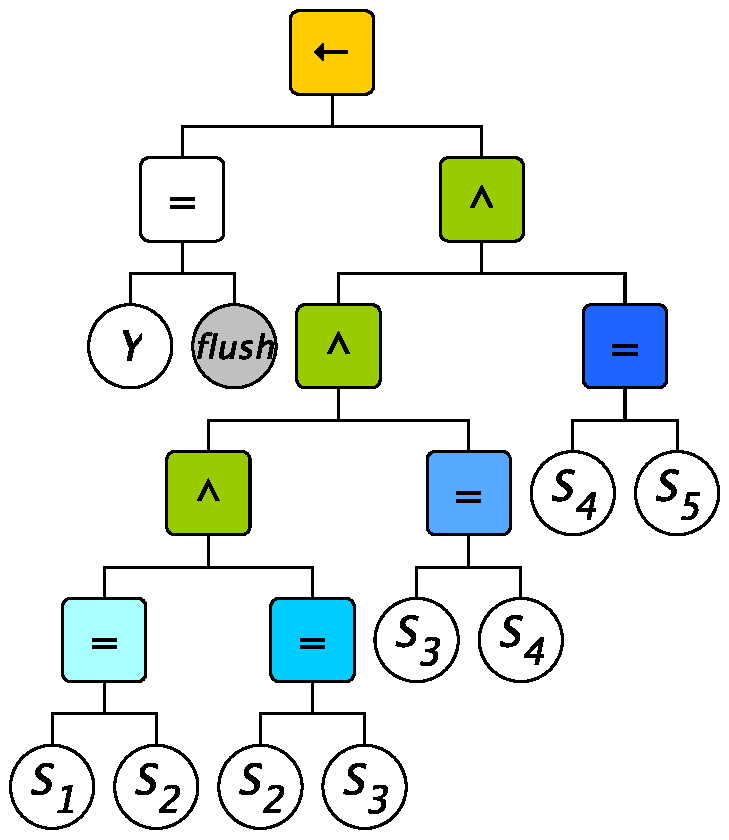
\includegraphics[width=\linewidth]{figures/ast-flush-1.pdf}
        \caption{AST of a formula}
        \label{fig:ast-kins-unencoded}
    \end{subfigure}
    \hfill$\rightarrow$\hfill
    \begin{subfigure}[]{0.32\linewidth}
        \centering
        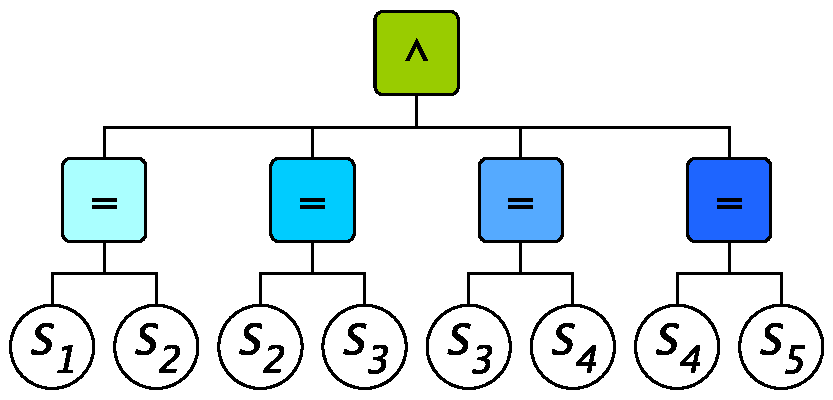
\includegraphics[width=\linewidth]{figures/ast-flush-2.pdf}
        \caption{Optimised AST of a formula}
        \label{fig:ast-kins-optimised}
    \end{subfigure}
    \hfill$\rightarrow$\hfill
    \begin{subfigure}[]{0.35\linewidth}
        \centering
        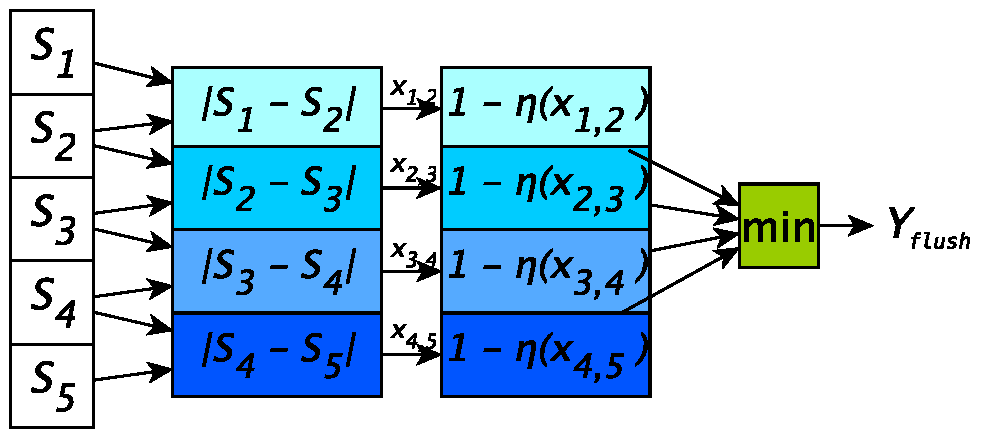
\includegraphics[width=\linewidth]{figures/net-flush.pdf}
        \caption{Layers from the optimised AST}
        \label{fig:net-kins-encoded}
    \end{subfigure}
    \caption[KINS Encoding of logic formulas into module networks]{
        %
        Example of the encoding process of formulas into module network.
        %
        Box coloured in the same way represent the encoding of a given operator through each encoding step.
    }
    \label{fig:ast-kins}
\end{figure*}

%
\begin{figure}
    \centering
    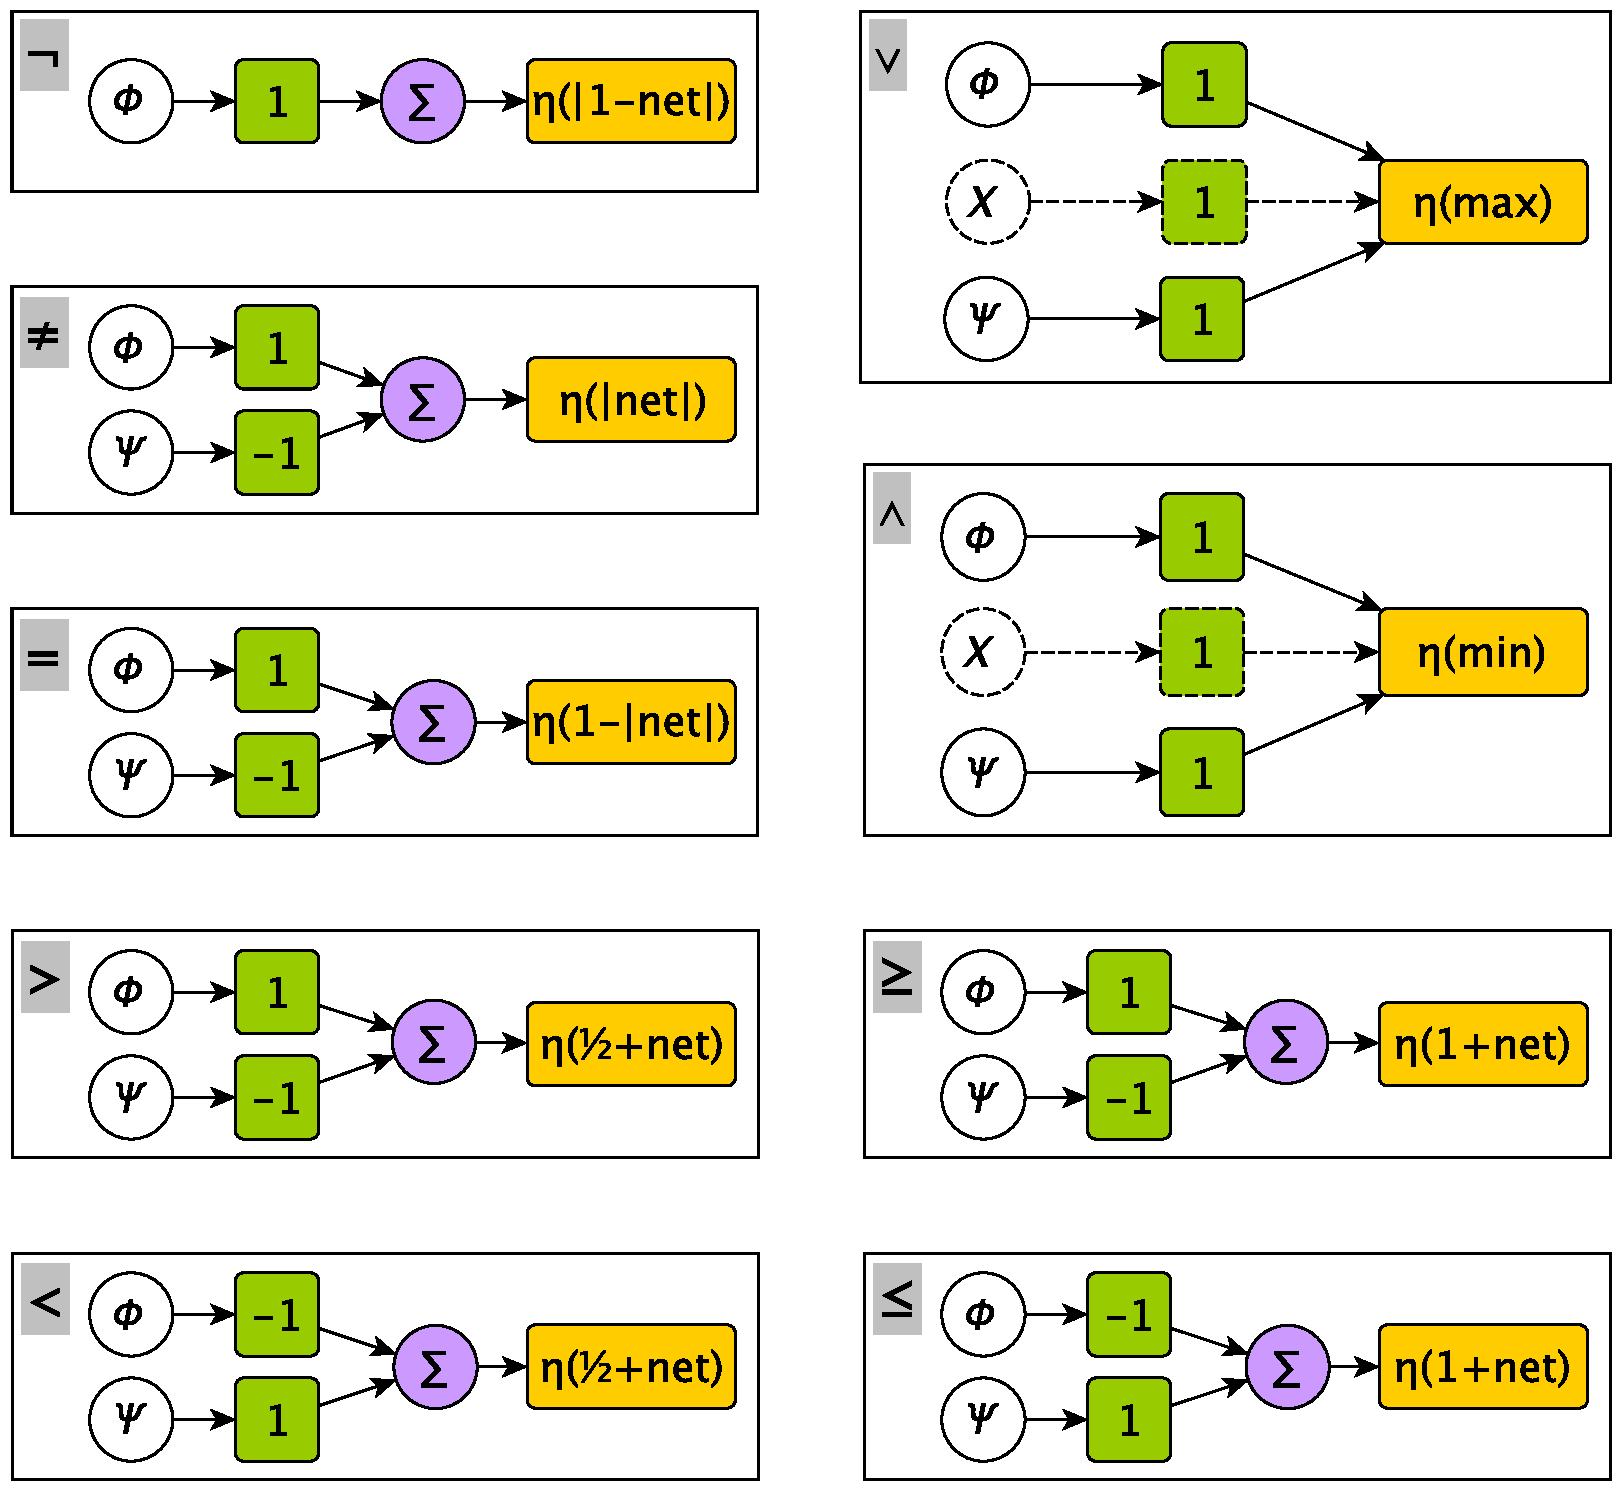
\includegraphics[width=0.8\linewidth]{figures/neurons}
    \caption[KINS mapping of formulas into neurons]{
        %
        \gls{KINS} mapping of formulas into neurons.
        %
        White circles are input variables ($I$), green boxes represent the corresponding weights ($W$), purple circles are the sum of the weighted inputs ($W x I$).
        %
        Yellow rectangles are activation functions, net is the output of $W x I$, maz and min respectively the maximum and minimum of input values, $\eta$ is the function described in \Cref{eq:eta-function}.
    }
    \label{fig:kins-neurons-mapping}
\end{figure}
%
By considering the same domain of the \gls{PHDS} used in \Cref{subsec:kill-validation}, we can take \Cref{eq:flush-class} as an example of a formula to be injected.
%
The procedure for encoding a logic formula into a dedicated neural module is illustrated in \Cref{fig:ast-kins}.
%
In this example, \Cref{eq:flush-class} is transformed into a neural module through three distinct phases.
%
First, the logic formula is parsed to construct its \gls{AST}, as shown in \Cref{fig:ast-kins-unencoded}.
%
Second, the \gls{AST} is simplified by merging commutative binary operators, as depicted in \Cref{fig:ast-kins-optimised}.
%
Third, the simplified \gls{AST} is encoded into a neural network, where each operator is mapped to a neuron that implements the corresponding operation, as specified in \Cref{tab:kins-logic-formulae}.
%
During the final step, the encoding rules defined in \Cref{fig:kins-neurons-mapping} are recursively applied to convert operators into neurons.
%
Input variables, such as \(S_i\), are represented as input neurons, while constants appearing in the formulas are mapped to neurons with fixed outputs.
%
Additionally, algebraic operations, including addition and multiplication, are implemented using single neurons that perform the respective operations.
%
This approach ensures that the symbolic knowledge is seamlessly integrated into the neural network structure.
%
A public implementation of the \gls{KINS} algorithm is available as part of the \gls{PSyKI}~\cite{DBLP:conf/atal/MagniniCO22} library$^\text{\ref{foot:psyki}}$.


\subsection{Validation}\label{subsec:kins-validation}
%
\begin{table}
    \centering
    \begin{adjustbox}{width=\linewidth, center}
        \begin{tabular}{c||c|c|c|c||l}
            \textbf{Symbol} & \textbf{Adenine} & \textbf{Cytosine} & \textbf{Guanine} & \textbf{Thymine} & \textbf{Logic form}
            \\
            \hline\hline
            $\const{d}$ & \yes & & \yes & \yes & $(\var{X}_i = \const{d}) \equiv (\var{X}_i = \const{a} \vee \var{X}_i = \const{g} \vee \var{X}_i = \const{t})$
            \\\hline
            $\const{m}$ & \yes & \yes & & & $(\var{X}_i = \const{m}) \equiv (\var{X}_i = \const{a} \vee \var{X}_i = \const{c})$
            % \\\hline
            % $\const{n}$ & \yes & \yes & \yes & \yes
            \\\hline
            $\const{r}$ & \yes & & \yes & & $(\var{X}_i = \const{r}) \equiv (\var{X}_i = \const{a} \vee \var{X}_i = \const{g})$
            \\\hline
            $\const{s}$ & & \yes & \yes & & $(\var{X}_i = \const{s}) \equiv (\var{X}_i = \const{c} \vee \var{X}_i = \const{g})$
            \\\hline
            $\const{y}$ & & \yes & & \yes & $(\var{X}_i = \const{y}) \equiv (\var{X}_i = \const{c} \vee \var{X}_i = \const{t})$
        \end{tabular}
    \end{adjustbox}
    \caption{
        Mapping of aggregative symbols and the four nucleotides.
        %
        Each symbol can be substituted with one base on the right that has a dot.
    }
    \label{tab:dna-symbols}
\end{table}
%
In this section, we evaluate the performance of \gls{KINS} in improving the predictive capabilities of \glspl{NN} through \gls{SKI}.
%
To ensure reproducibility, the code used for our experiments is publicly available\footnote{\url{https://github.com/MatteoMagnini/kins-experiments-cilc-2022}}.
%
The validation is conducted using the well-known \gls{PSJGS} dataset~\cite{splice-junction_gene_sequences_69}.
%
This dataset consists of 3190 records, each representing a sequence of 60 DNA nucleotides.
%
The nucleotides are adenine (\texttt{a}), cytosine (\texttt{c}), guanine (\texttt{g}), and thymine (\texttt{t}).
%
Auxiliary symbols are used to denote multiple possible nucleotides in a compact way, as shown in \Cref{tab:dna-symbols}.
%
Each sequence spans positions from -30 to +30, excluding position 0.
%
The classification task involves identifying whether a sequence corresponds to an \gls{IE} boundary, an \gls{EI} boundary, or neither (N).
%
The dataset is imbalanced, with class frequencies distributed as follows: 50\% for N, and 25\% each for \gls{IE} and \gls{EI}.
%
This imbalance poses challenges for accurate classification, making it a suitable benchmark for testing \gls{KINS}.


\paragraph{\gls{PSJGS} logic rules}\label{par:kins-psjgs-logic-rules}
%
\begin{table}
    \centering
    \begin{adjustbox}{width=\linewidth, center}
        \begin{tabular}{c|p{\linewidth-4cm}}
            \textbf{Class} & \textbf{Logic Formulation}
            \\\hline\hline
            \emph{EI} & $\begin{array}{l}
                \begin{aligned}
                    \\
                    \pred{class}(\bar{\var{X}}, \const{ei}) \leftarrow& \var{X}_{-3} = \const{m} \wedge \var{X}_{-2} = \const{a} \wedge \var{X}_{-1} = \const{g} \wedge \var{X}_{+1} = \const{g}\ \wedge\\
                    & \var{X}_{+2} = \const{t} \wedge \var{X}_{+3} = \const{a} = \const{r} \wedge \var{X}_{+4} = \const{a}\ \wedge \\
                    & \var{X}_{+5} = \const{g} \wedge \var{X}_{+6} = \const{t} \wedge \neg(\pred{ei\_stop}(\bar{\var{X}}))
                \end{aligned}
                \\
                \pred{ei\_stop}(\bar{\var{X}}) \leftarrow \var{X}_{-3} = \const{t} \wedge \var{X}_{-2} = \const{a} \wedge \var{X}_{-1} = \const{a}
                \\
                \pred{ei\_stop}(\bar{\var{X}}) \leftarrow \var{X}_{-3} = \const{t} \wedge \var{X}_{-2} = \const{a} \wedge \var{X}_{-1} = \const{g}
                \\
                \pred{ei\_stop}(\bar{\var{X}}) \leftarrow \var{X}_{-3} = \const{t} \wedge \var{X}_{-2} = \const{g} \wedge \var{X}_{-1} = \const{a}
                \\
                \pred{ei\_stop}(\bar{\var{X}}) \leftarrow \var{X}_{-4} = \const{t} \wedge \var{X}_{-3} = \const{a} \wedge \var{X}_{-2} = \const{a}
                \\
                \pred{ei\_stop}(\bar{\var{X}}) \leftarrow \var{X}_{-4} = \const{t} \wedge \var{X}_{-3} = \const{a} \wedge \var{X}_{-2} = \const{g}
                \\
                \pred{ei\_stop}(\bar{\var{X}}) \leftarrow \var{X}_{-4} = \const{t} \wedge \var{X}_{-3} = \const{g} \wedge \var{X}_{-2} = \const{a}
                \\
                \pred{ei\_stop}(\bar{\var{X}}) \leftarrow \var{X}_{-5} = \const{t} \wedge \var{X}_{-4} = \const{a} \wedge \var{X}_{-3} = \const{a}
                \\
                \pred{ei\_stop}(\bar{\var{X}}) \leftarrow \var{X}_{-5} = \const{t} \wedge \var{X}_{-4} = \const{a} \wedge \var{X}_{-3} = \const{g}
                \\
                \pred{ei\_stop}(\bar{\var{X}}) \leftarrow \var{X}_{-5} = \const{t} \wedge \var{X}_{-4} = \const{g} \wedge \var{X}_{-3} = \const{a}
                \\
            \end{array}$
            \\
            \\
            \hdashline
            \\
            \emph{IE} & $\begin{array}{l}
                \begin{aligned}
                  \pred{class}(\bar{\var{X}}, \const{ie}) \leftarrow &\pred{pyramidine\_rich}(\bar{\var{X}}) \wedge \neg(\pred{ie\_stop}(\bar{\var{X}}))\ \wedge\\
                    & \var{X}_{-3} = \const{y} \wedge \var{X}_{-2} = \const{a} \wedge \var{X}_{-1} = \const{g} \wedge \var{X}_{+1} = \const{g}
                \end{aligned}
                \\
                \pred{pyramidine\_rich}(\bar{\var{X}}) \leftarrow 6 \le (\var{X}_{-15} = \const{y} + \ldots + \var{X}_{-6} = \const{y})
                \\
                \pred{ie\_stop}(\bar{\var{X}}) \leftarrow \var{X}_{+2} = \const{t} \wedge \var{X}_{+3} = \const{a} \wedge \var{X}_{+4} = \const{a}
                \\
                \pred{ie\_stop}(\bar{\var{X}}) \leftarrow \var{X}_{+2} = \const{t} \wedge \var{X}_{+3} = \const{a} \wedge \var{X}_{+4} = \const{g}
                \\
                \pred{ie\_stop}(\bar{\var{X}}) \leftarrow \var{X}_{+2} = \const{t} \wedge \var{X}_{+3} = \const{g} \wedge \var{X}_{+4} = \const{a}
                \\
                \pred{ie\_stop}(\bar{\var{X}}) \leftarrow \var{X}_{+3} = \const{t} \wedge \var{X}_{+4} = \const{a} \wedge \var{X}_{+5} = \const{a}
                \\
                \pred{ie\_stop}(\bar{\var{X}}) \leftarrow \var{X}_{+3} = \const{t} \wedge \var{X}_{+4} = \const{a} \wedge \var{X}_{+5} = \const{g}
                \\
                \pred{ie\_stop}(\bar{\var{X}}) \leftarrow \var{X}_{+3} = \const{t} \wedge \var{X}_{+4} = \const{g} \wedge \var{X}_{+5} = \const{a}
                \\
                \pred{ie\_stop}(\bar{\var{X}}) \leftarrow \var{X}_{+4} = \const{t} \wedge \var{X}_{+5} = \const{a} \wedge \var{X}_{+6} = \const{a}
                \\
                \pred{ie\_stop}(\bar{\var{X}}) \leftarrow \var{X}_{+4} = \const{t} \wedge \var{X}_{+5} = \const{a} \wedge \var{X}_{+6} = \const{g}
                \\
                \pred{ie\_stop}(\bar{\var{X}}) \leftarrow \var{X}_{+4} = \const{t} \wedge \var{X}_{+5} = \const{g} \wedge \var{X}_{+6} = \const{a}
                \\
            \end{array}$
        \end{tabular}
    \end{adjustbox}
    \caption{Datalog formul\ae{} describing DNA classification criteria generated from the original one.}
    \label{tab:dna-rules}
\end{table}

%
\begin{figure}
    \centering
    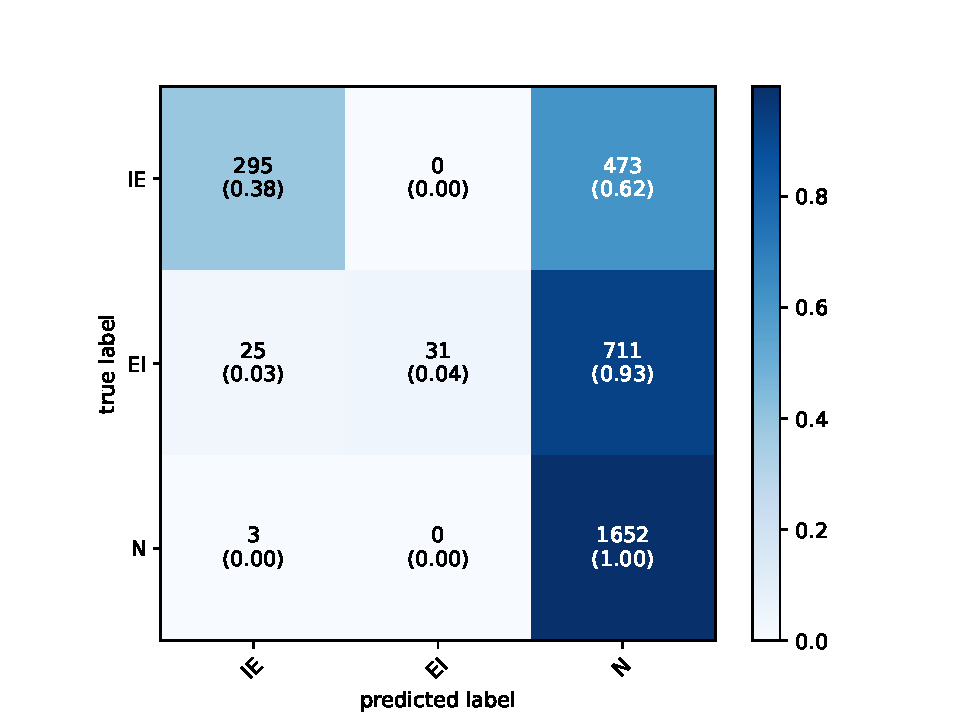
\includegraphics[width=0.8\linewidth]{figures/psjgs-rules-confusion-matrix}
    \caption[Confusion matrix of the knowledge for the PSJGS dataset]{
        %
        Confusion matrix of the knowledge for the \gls{PSJGS} dataset.
        %
        The matrix shows the classification results of the knowledge rules on the dataset if applied directly.
    }
    \label{fig:psjgs-rules-confusion-matrix}
    %
\end{figure}
%
The \gls{PSJGS} dataset includes a set of textual logical rules designed by human experts to classify DNA sequences.
%
\Cref{tab:dna-rules} presents these rules converted into Datalog form, which is equivalent to the original custom formalism but machine-interpretable.
%
In Datalog, variables are indexed from $-30$ to $30$, excluding position $0$.
%
Each variable $X_{\pm i}$ represents the nucleotide at position $\pm i$, encoded using constants such as \texttt{a}, \texttt{c}, \texttt{g}, and \texttt{t}.
%
For simplicity, the notation $\bar{X}$ is used to represent the full sequence of variables $X_{-30}, \dots, X_{-1}, X_{+1}, \dots, X_{+30}$.

The original rules also utilize additional symbols to compactly represent multiple possible nucleotides.
%
\Cref{tab:dna-symbols} provides the mapping of these symbols to their corresponding nucleotide combinations.

When applying the rules in \Cref{tab:dna-rules} to classify sequences in the \gls{PSJGS} dataset, sequences of type \gls{IE} are correctly classified $295$ times as \gls{TP}.
%
However, the same rule also incorrectly classifies $25$ \gls{EI} sequences and $3$ N sequences as \gls{FP}.
%
In contrast, \gls{EI} sequences are correctly classified $31$ times, with no \gls{FP}.

To address the classification of sequences of type N, a fictional rule is introduced, which negates both \gls{IE} and \gls{EI} rules:
%
\begin{align}
    \pred{class}(\bar{X}, \const{n}) &\leftarrow \neg \pred{class}(\bar{X}, \const{ei}) \land \neg \pred{class}(\bar{X}, \const{ie}).
\end{align}

\Cref{fig:psjgs-rules-confusion-matrix} shows the confusion matrix of the knowledge rules applied to the dataset.
%
Although these rules do not perfectly describe the domain, they are sufficiently accurate to positively influence the training of the predictor.
%
Further refinements or additional rules may improve the classification performance.


\paragraph{Methodology}\label{par:kins-psjgs-methodology}
%
To ensure comparability with existing literature benchmarks, we adopt the methodology proposed by Towell and Shavlik~\cite{DBLP:journals/ai/TowellS94}.
%
Specifically, we perform 10-fold cross-validation using a training set of $1,000$ randomly selected records from the $3,190$ available ones, which corresponds to $31.3\%$ of the dataset.
%
For each fold, we train one instance of \gls{KINS}.
%
The test accuracy is computed on the remaining $2,190$ records by averaging the predictions of the $10$ trained \gls{KINS} instances.
%
Unlike the original method, we repeat the experiment $30$ times instead of $10$ to improve statistical significance.

Each \gls{KINS} instance is trained using a fully connected \gls{NN} with three layers.
%
The input layer consists of $60$ neurons, the hidden layer has a configurable number of neurons, and the output layer includes $3$ neurons corresponding to the classification task.
%
To mitigate overfitting, we apply dropout~\cite{DBLP:journals/jmlr/SrivastavaHKSS14} with a rate of $0.2$ to each layer during training.
%
The activation function for the hidden layers is \gls{ReLU}, while the output layer uses the softmax function.
%
The network is optimized using the Adam optimizer~\cite{DBLP:journals/corr/KingmaB14} and categorical cross-entropy as the loss function.

We employ the stopping criteria described in~\cite{DBLP:journals/ai/TowellS94}.
%
These criteria include ensuring that $99\%$ of the training examples have output activations within $0.25$ of the correct value, limiting training to a maximum of $100$ epochs, and stopping when the predictor achieves at least $90\%$ accuracy on the training examples but shows no improvement for five consecutive epochs.

The rules $\pred{ei\_stop}(\bar{\var{X}})$ and $\pred{ie\_stop}(\bar{\var{X}})$ are immutable, meaning their weights remain fixed during training.
%
In contrast, the rules $\pred{class}(\bar{\var{X}}, \const{ei})$, $\pred{class}(\bar{\var{X}}, \const{ie})$, and $\pred{pyramidine\_rich}(\bar{\var{X}})$ are mutable, allowing their weights to be adjusted during training.
%
Immutable rules preserve their structure, while mutable rules adapt to the data to improve predictive performance.



\paragraph{Results and discussion}\label{par:kins-psjgs-results}
%
\begin{figure}
    \centering
    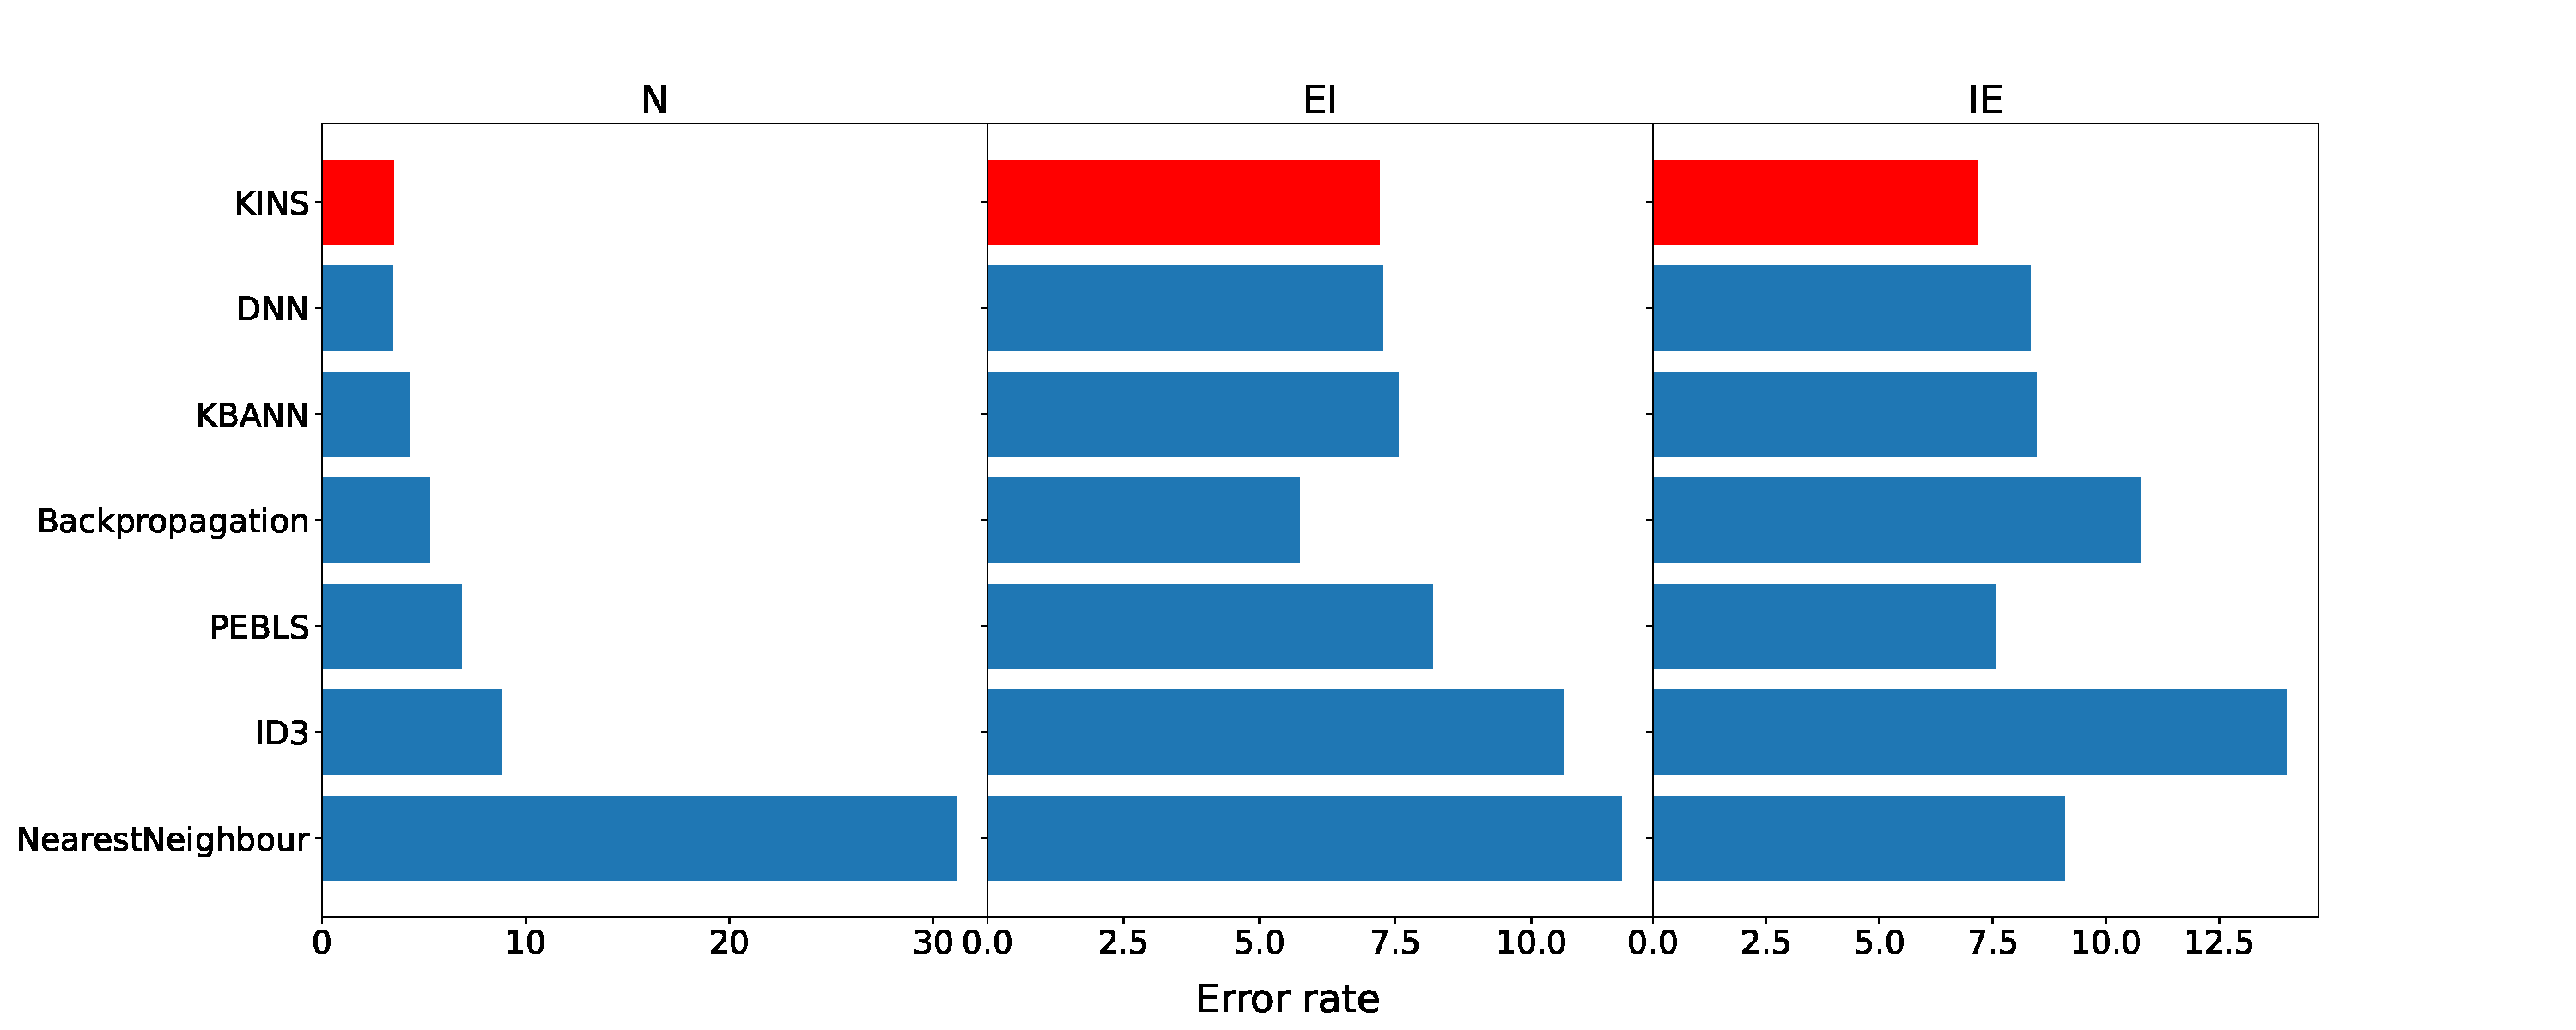
\includegraphics[width=\linewidth]{figures/psjgs-kins-error-rate}
    \caption[KINS PSJGS error rate]{
        %
        Error rate per class for the \gls{PSJGS} dataset using \gls{KINS}.
        %
        The results are compared with other algorithms, including DNN (the network used in KINS without knowledge injection) and KBANN~\cite{DBLP:journals/ai/TowellS94}.
        %
        The error rate is significantly lower for \gls{KINS} compared to DNN and KBANN.
    }
    \label{fig:kins-psjgs-error-rate}
\end{figure}
%
We evaluate \gls{KINS} by injecting prior knowledge into different layers of the \gls{NN} described earlier.
%
The best results are achieved when the injection is performed at the first hidden layer.
%
Following the methodology outlined in \Cref{par:kins-psjgs-methodology}, we train $10$ predictors on $900$ records each, resulting in a total of $1,000$ unique training records out of $3,190$ for each experiment.
%
We conduct $30$ experiments using 10-fold cross-validation with random weight initialization.
%
After injecting prior knowledge into the first hidden layer and training, the mean accuracy across the $30$ experiments on the test set is \(94.73\%\).
%
The mean class accuracies are as follows: \gls{IE} \(92.79\%\), \gls{EI} \(92.49\%\), and N \(96.67\%\).

For comparison, we perform $30$ additional runs using the same base \gls{NN} architecture without injecting any knowledge.
%
The results are: mean accuracy \(94.45\%\), \gls{IE} \(91.67\%\), \gls{EI} \(92.73\%\), and N \(96.54\%\).
%
Using Student's \(t\)-test, we reject the null hypothesis, confirming that predictors generated with \gls{KINS} achieve statistically significant improvements in accuracy.
%
The accuracy improvement using \gls{KINS} is notable even when the injected knowledge is imperfect.

\Cref{fig:kins-psjgs-error-rate} illustrates the error rate per class for different algorithms.
%
\gls{KINS} represents our knowledge injection method, while \gls{DNN} refers to the same network used in \gls{KINS} without knowledge injection.
%
\Gls{KBANN}, as proposed in~\cite{DBLP:journals/ai/TowellS94}, performs slightly worse than both \gls{DNN} and \gls{KINS}.
%
The primary reason for this difference is that \gls{KBANN} fully reflects the provided knowledge in its structure, whereas \gls{KINS} allows a portion of the network to adapt to the data.
%
This flexibility is advantageous when the knowledge closely aligns with the domain rules but can be a limitation in the opposite scenario.
%
Other algorithms, including standard backpropagation~\cite{rumelhart1987learning}, \gls{PEBLS}~\cite{DBLP:journals/ml/CostS93}, ID3~\cite{quinlan1986induction}, and nearest neighbors, generally perform worse than \gls{KINS}.


% \section{Discussion and future direction}\label{sec:ski-discussion-and-future-direction}
%! Author = matteomagnini
%! Date = 05/03/25

%----------------------------------------------------------------------------------------
\chapter[Platform for symbolic knowledge injection]{\Glsentrylong{PSyKI}}
\label{ch:psyki}
\minitoc
%----------------------------------------------------------------------------------------

In this chapter, we present the \Gls{PSyKI} platform, which is a framework for \gls{SKI} methods.
%
\Gls{PSyKI} provides a unified way to implement \gls{SKI} methods, aiming to facilitate the development and comparison of different approaches.
%
It also provides a set of tools to evaluate the performance of \gls{SKI} methods, including metrics for measuring the quality of the injected knowledge and the performance of the resulting models.
%
In \Cref{sec:psyki}, we present the work ``\emph{On the Design of PSyKI: A Platform for Symbolic Knowledge Injection into Sub-symbolic Predictors}''~\cite{DBLP:conf/atal/MagniniCO22}, which describes the design and implementation of \gls{PSyKI}.
%
Then, in \Cref{sec:ski-meets-intelligent-agents,sec:empirical-study-on-the-robustness-of-ski-methods}, we present respectively two works that study the quality of service of \gls{SKI} methods:
%
in \Cref{sec:ski-meets-intelligent-agents} the paper ``\emph{Symbolic Knowledge Injection Meets Intelligent Agents}''~\cite{DBLP:journals/aamas/AgiolloRMCO23},
%
which introduces metrics for evaluating the performance of \gls{SKI} methods in the context of intelligent agents,
%
and in \Cref{sec:empirical-study-on-the-robustness-of-ski-methods} the paper ``\emph{An Empirical Study on the Robustness of Symbolic Knowledge Injection Techniques Against Data Degradation}''~\cite{DBLP:conf/woa/RafanelliMACO24},
%
which studies the robustness of \gls{SKI} methods against data degradation.


\section{PSyKI}\label{sec:psyki}
%
\Gls{PSyKI} is a (Python) platform for the development and evaluation of \gls{SKI} methods.
%
It is designed to provide a unified framework for implementing \gls{SKI} methods, allowing researchers and practitioners to easily develop, test, and compare different approaches.
%
In the following, we present a summary of the work ``\emph{On the Design of PSyKI: A Platform for Symbolic Knowledge Injection into Sub-symbolic Predictors}''~\cite{DBLP:conf/atal/MagniniCO22}, presented at the 4th international workshop on \gls{EXTRAAMAS}, 2022\footnote{\url{https://extraamas.ehealth.hevs.ch/archive.html}}.
%
The library is public available on GitLab and PyPi\footnote{\url{https://gitlab.com/psykei/psyki-python} and \url{https://pypi.org/project/psyki/}}.


\subsection{Motivations}\label{subsec:psyki-motivations}
%
This work is motivated by the need to address the common challenges that affect \gls{SKI} methods (see \Cref{subsec:limitations-and-challenges-of-ski}).
%
In particular, we want to address the following points:
%
\begin{inlinelist}
    \item \emph{lack of generality}, by providing the proper tools to automatically translate symbolic knowledge of arbitrary domains into a format suitable for injection into sub-symbolic predictors,
    %
    \item \emph{lack of reproducibility}, by providing a unified framework for implementing \gls{SKI} methods, allowing researchers to easily develop, test, and compare different approaches, and
    %
    \item \emph{lack of availability}, by encouraging the development of reusable software libraries for \gls{SKI} methods.
    %
\end{inlinelist}
%
Concerning the last point mentioned in \Cref{subsec:limitations-and-challenges-of-ski}, we identified in the logic language of stratified Datalog with negation a suitable candidate for the symbolic knowledge representation.
%
It is expressive enough to represent a wide range of symbolic knowledge, while being simple enough to be easily translated into a format suitable for injection into sub-symbolic predictors.


\subsection{Design}\label{subsec:design-and-implementation}
%
\begin{figure}
    \centering
    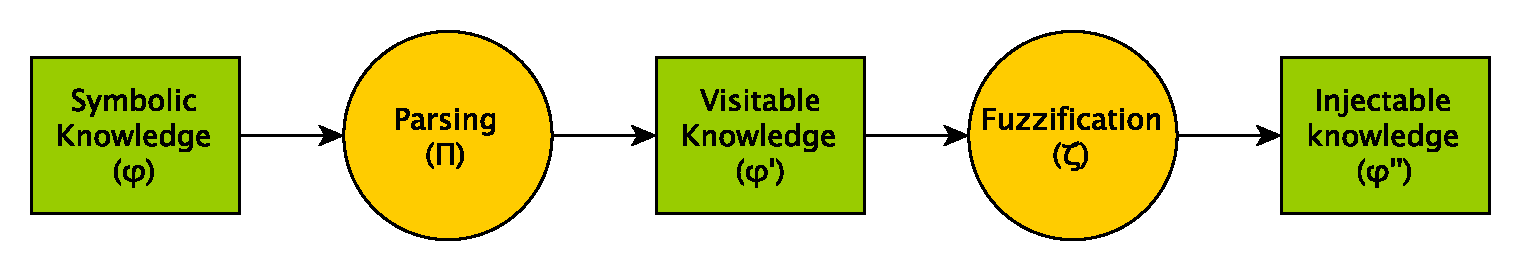
\includegraphics[width=\textwidth]{figures/knowledge-workflow-psyki}
    \caption[Symbolic knowledge transformation in PSyKI]{
        General workflow of symbolic knowledge transformation in \Gls{PSyKI}.
        The symbolic knowledge ($\phi$), typically expressed as logical formulas, is first parsed into a visitable form ($\phi'$), and then fuzzified into a machine-injectable representation ($\phi''$).
    }
    \label{fig:knowledge-workflow-psyki}
\end{figure}
%
All symbolic knowledge injection (\gls{SKI}) methods implemented in \gls{PSyKI} share a common transformation pipeline, illustrated in \Cref{fig:knowledge-workflow-psyki}.
%
Symbolic knowledge \(\phi\) cannot usually be injected directly into a sub-symbolic predictor.
%
Instead, it undergoes a two-step transformation:
%
\begin{inlinelist}
    %
    \item \emph{Parsing} (\(\Pi\)): the knowledge is converted into a visitable data structure, such as an \gls{AST} in the case of logic formulas, resulting in \(\phi'\);
    %
    \item \emph{Fuzzification} (\(\zeta\)): the parsed representation is transformed into a sub-symbolic form \(\phi''\), suitable for injection.
    %
\end{inlinelist}
%
Fuzzification plays a key role in bridging the symbolic and sub-symbolic domains.
%
It translates crisp Boolean logic into a form compatible with sub-symbolic models, often by relaxing discrete truth values into continuous-valued functions or generating neural components such as layers or entire \glspl{NN}.

\begin{figure}
    \centering
    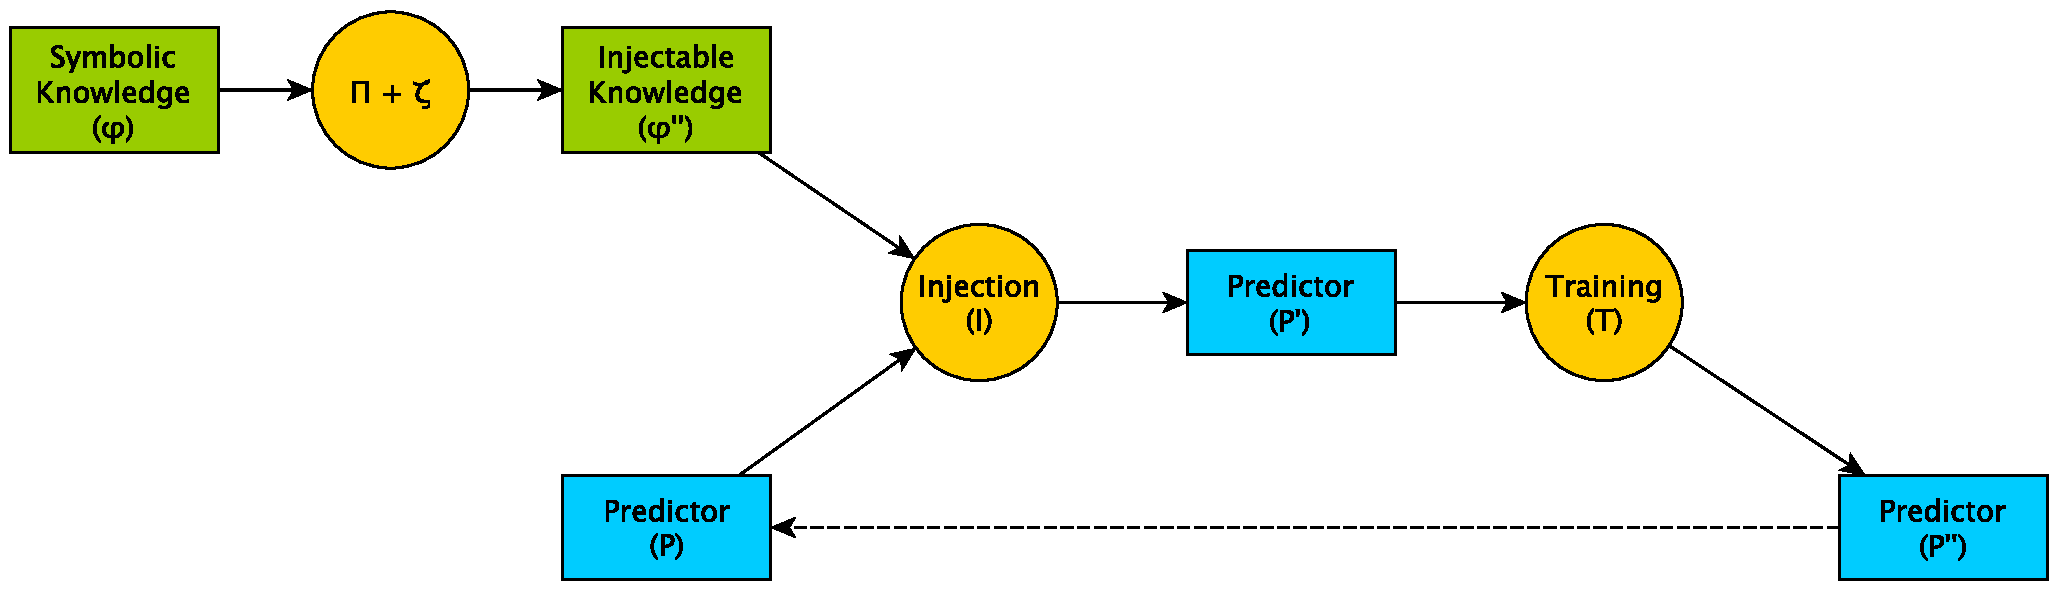
\includegraphics[width=\textwidth]{figures/psyki-workflow}
    \caption[General workflow of PSyKI]{
        Complete workflow of structuring and guided learning \gls{SKI} methods in \Gls{PSyKI}.
        The symbolic knowledge is transformed and injected into the sub-symbolic predictor, which is then trained on data.
    }
    \label{fig:psyki-workflow}
\end{figure}
%
\Cref{fig:psyki-workflow} shows the overall injection process in \gls{PSyKI}, including both the transformation of the symbolic knowledge and its integration into the learning system.
%
After the transformation phase, the different \gls{SKI} methods diverge:
%
\begin{inlinelist}
    %
    \item \emph{Structuring} and \emph{guided learning} inject \(\phi''\) directly into the architecture or training process of the predictor;
    %
    \item \emph{Embedding}-based methods use symbolic knowledge to enrich or generate the input data, so they are not directly represented in \Cref{fig:psyki-workflow}.
    %
\end{inlinelist}

\Gls{PSyKI} supports all three approaches, although it is primarily designed for \emph{structuring} and \emph{guided learning}, where the injection occurs directly into the predictor.
%
In general, \gls{SKI} algorithms operate on a predictor \(P\) and symbolic knowledge \(\phi\), producing a new predictor \(P'\) as output.
%
This modified predictor is then trained on data, resulting in a final model \(P''\), which can be reused in further iterations with different knowledge or injection strategies.


\paragraph{Architecture}\label{par:architecture}
%
\begin{figure}
    \centering
    \includegraphics[width=\textwidth]{figures/class-diagram}
    \caption[Class diagram of PSyKI]{
        Class diagram of \Gls{PSyKI}.
        %
        The main components are the \emph{Injector}, the \emph{Formula} and the \emph{Fuzzifier}.
        %
        The package \emph{logic.datalog} is an examplification showing two \emph{Injector} implementations and their relationships.
    }
    \label{fig:psyki-class-diagram}
\end{figure}
%
Essentially, \gls{PSyKI} is designed around the notion of injector.
%
An injector is any algorithm accepting a \gls{ML} predictor and prior symbolic knowledge -- predominantly logic formulas -- as input that produces a new predictor as output.
%
In order to properly perform injection, injectors may require additional information such as algorithm specific hyperparameters.


\gls{PSyKI} supports the processing of symbolic knowledge represented via logic formulas.
%
Based on the sort of logic, user can build an \gls{AST} for each formula.
%
The \gls{AST} can be inspected through a fuzzifier via pattern visitor to encode the symbolic knowledge to a sub-symbolic form (e.g. fuzzy logic functions, ad-hoc layers).
%
The resulting sub-symbolic object can finally be used by an injector to create a new predictor.
%
This process -- denoted with $\zeta$ \Cref{fig:psyki-workflow} -- is injector specific; instead, the same parser $\Pi$ can be used for logic formulas of the same sort independently of the injector.


The software is organized into well-separated packages to ensure easy extensibility towards new sort of logic and fuzzifiers---see \Cref{fig:psyki-class-diagram}
%
An \gls{AST} is a \emph{formula} object, and it can have different language specific elements w.r.t. the logic form that is covered.
%
Each formula implementation is self-contained inside a standalone package so that if a user wants to add a new logic form it is sufficient to add its implementation in a new package.
%
Similarly, a fuzzifier object that targets a specific logic form can be added inside the same package of the logic, there can be any number of fuzzifiers for a given logic.


\subsection{Implementation}\label{subsec:psyki-implementation}
%
\paragraph{Knowledge representation}\label{par:knowledge-representation}
%
\begin{figure}
    \centering
    \includegraphics[width=\textwidth]{figures/grammar}
    \caption[Class diagram for the representation of Datalog formulas]{
        A supported grammar of \Gls{PSyKI} for logic formulas.
        %
        The grammar is designed to represent Datalog formulas.
    }
    \label{fig:grammar}
\end{figure}
%
A crucial point in the \gls{SKI} workflow is the embedding of knowledge from symbolic into sub-symbolic form.
%
Ideally, there is no constraint on the formalism used to represent the prior knowledge (e.g., logic formulas, knowledge graph).
%
The most common knowledge representation form that \gls{SKI} algorithms claim to support is \gls{FOL} or one of its subsets.
%
However, there are characteristics of \gls{FOL} that are not ideal for some predictors.
%
Recursion and function symbols -- that allow recursive structures -- cannot be easily integrated into a predictor that is acyclic -- i.e., no recursive -- by construction such as conventional \gls{NN} (virtually all \gls{NN}, with few exceptions like fibred \gls{NN}~\cite{DBLP:conf/flairs/BaderGH05}).
%
Conversely, in this work we consider one of the most general and expressive logic formalism that does not support recursion and function symbols: stratified Datalog with negation.


Stratified Datalog with negation has been already described in detail in \Cref{subsec:ski-stratified-datalog-with-negation}.
%
To support injection into a particular predictor, we further assume the input knowledge base defines at least one outer relation -- say output or class -- involving as many variables as the input and output features the predictor has been trained upon.
%
Such a relation may be defined via one or more clauses, and each clause may leverage on other predicates in their bodies.
%
In turn, each predicate may be defined through one or more clause.
%
In that case, since we rely on stratified Datalog, we require input knowledge to not include any (directly or indirectly) recursive clause definition.


Once that the logic has been formalized, the implementation of a \emph{Formula} -- visitable data structure like an \gls{AST} -- is quite straightforward.
%
\Cref{fig:grammar} depicts the general API for representing logic formulas, as currently supported by \gls{PSyKI}.
%
To make \gls{PSyKI} able to parse bare text into actual logic formulas compliant to that API, we rely on well-established parser-generation facilities such as ANTLR~\cite{DBLP:journals/spe/ParrQ95}.
%
As further discussed below, the knowledge contained into a Formula object, can then be embedded in sub-symbolic form, via a fuzzifier, to be later injected into a predictor.


Later in the evolution of \gls{PSyKI} (i.e., from v. 0.2.1), we considered switching to a more established logic language for representing the symbolic knowledge: Prolog~\cite{DBLP:journals/tplp/KornerLBCDHMWDA22}.
%
In particular, we abandoned the manual parsing of logic formulas with ANTLR, and we rely on the tuProlog~\cite{DBLP:conf/padl/DentiOR01} framework.
%
We use the parser of tuProlog to parse the logic formulas, but \gls{PSyKI} does not support the full Prolog language because of the limitations of injecting into \gls{NN} mentioned in \Cref{subsec:limitations-and-challenges-of-ski} (i.e., we still support only stratified Datalog with negation).


\paragraph{Fuzzification}\label{par:fuzzification}
%
While logic formulas are commonly interpreted in a Boolean way -- i.e., they can be assigned with one truth value among true and false --, sub-symbolic predictors are more flexible-hence supporting formulas to hold up to some extent.
%
Switching from the former interpretation to the latter is, essentially, the purpose of fuzzifiers.
%
In practice, this implies converting a logic formula into a function of real numbers.
%
Along this line, fuzzification may be performed in (at least) two ways; real numbers may either represent
%
\begin{inlinelist}
    %
    \item a \emph{penalty} for the violation of a formula, or
    %
    \item the \emph{degree of truth} of that formula.
    %
\end{inlinelist}

To serve this purpose, one may rely on a multivalued interpretation of logic inspired to $\L$ukasiewicz's logic, where the value true is represented by 0 (resp. 1), while higher (resp. lower) values represent ``falsity''.
%
In particular, this approach may be useful to constrain a predictor during its training.
%
Examples of this fuzzification approach are \gls{KILL} (\Cref{subsec:kill-fuzzifier}) and \gls{KINS} (\Cref{subsec:kins-fuzzifier}).
%
\Cref{tab:kill-logic-formulae,tab:kins-logic-formulae} show the logic formulas encoding into real-valued functions for \gls{KILL} and \gls{KINS}, implementing \emph{penalty} and \emph{degree of truth} respectively.


\paragraph{Injection}\label{par:injection}
%
\lstinputlisting[
    basicstyle=\fontsize{8}{9.5}\ttfamily\selectfont,
    label=lst:psyki-injection,
    float,
    caption={General code snippet for the use of a \gls{SKI} method in the current version of \gls{PSyKI} (v. 0.4.3).},
    captionpos=b,
    language=Python,
]{listings/psyki-injection.py}
%
Knowledge injection is the central step in \gls{SKI}.
%
It is carried out by \emph{injectors}, i.e., objects wrapping a particular injection strategy.
%
Each injector is expected to accept one sub-symbolic predictors as input, other the logic formulas that should be injected into that predictor.
%
As part of its operation, the injector is in charge of producing a new predictor as output, of the same type as the one provided as input.
%
The new predictor is altered in such a way that it is consistent w.r.t. the provided logic formulas.


While the main architecture of \gls{PSyKI} has been maintained stable during the years, the implementation has been continuously improved.
%
The current version of \gls{PSyKI} (v. 0.4.3) is implemented in Python 3.9.13, with main dependencies being \texttt{tensorflow}, \texttt{2ppy}, \texttt{scikit-learn}, and \texttt{pandas}.
%
\Cref{lst:psyki-injection} shows a general code snippet for the use of a \gls{SKI} algorithm in \gls{PSyKI} (v. 0.4.3).


\section[SKI meets intelligent agents]{\Gls{SKI} meets intelligent agents}\label{sec:ski-meets-intelligent-agents}
%
In this and in the next section, we present two works that study the \gls{QoS} of \gls{SKI} methods.
%
\Gls{QoS} is a crucial aspect of any non-trivial systems, and it is particularly important for \gls{SKI} because the vast majority of the works in this field do not provide any evaluation but the performance of the resulting model.
%
Moreover, \gls{SKI} methods and the resulting educated models have many other dimensions that can be evaluated a part from the straight prediction performance.
%
The metrics introduced in these works have been implemented and integrated into \gls{PSyKI} from version 0.2.14 and later.


The work ``\emph{Symbolic Knowledge Injection Meets Intelligent Agents}''~\cite{DBLP:journals/aamas/AgiolloRMCO23}, published in the \emph{Autonomous Agents and Multi-Agent Systems} journal, presents a set of metrics for evaluating the performance of \gls{SKI} methods in the context of intelligent agents.
%
Here we present a summary of the work, including the motivations, the proposed metrics, and the evaluation of \gls{SKI} methods in terms of \gls{QoS}.


\subsection{Motivations}\label{subsec:ski-meets-intelligent-agents-motivations}
%
The current practice of assessing \gls{SKI} methods primarily focuses on measuring improvements in the predictive performance of an educated predictor \(\hat{N}\) over its uneducated counterpart \(N\).
%
However, predictive performance is not the only relevant benefit of \gls{SKI} that should be evaluated.

There are multiple aspects of \glspl{ML} predictors that can be influenced by \gls{SKI}, and for which specific metrics should be defined.
%
For instance, \gls{SKI} may impact the \emph{memory footprint}, \emph{latency}, \emph{data efficiency}, and \emph{energy consumption} of the predictors it is applied to.
%
Collectively, these properties contribute to what we refer to as the \emph{efficiency} of a predictor.

In this work, we consider the following efficiency properties:
%
\begin{properties}
    \item \textbf{Memory footprint}: the size of the predictor, typically measured in terms of the number of parameters or computational operations required.
    %
    \label{itm:memory-footprint}
    %
    \item \textbf{Latency}: the time required to perform a single inference.
    %
    \label{itm:latency}
    %
    \item \textbf{Data efficiency}: the amount of data required to train the predictor to achieve a certain level of performance.
    %
    \label{itm:data-efficiency}
    %
    \item \textbf{Energy consumption}: the energy required to train and/or run the predictor.
    %
    \label{itm:energy-consumption}
    %
    \item \textbf{Predictive performance}: standard metrics such as accuracy, F1-score, or mean squared error.
    %
    \label{itm:predictive-performance}
\end{properties}

For brevity, we refer to any function that measures one of these properties as an \emph{efficiency metric}.
%
These metrics quantify the improvement in a given property \(P\) of the uneducated predictor \(N\) when transformed into its educated counterpart \(\hat{N}\) through a \gls{SKI} mechanism.

The resulting efficiency scores can be influenced by several factors:
%
\begin{factors}
    %
    \item \textbf{Knowledge quality and coverage}:
    %
    The educated predictor \(\hat{N}\) is obtained by injecting symbolic knowledge \(K\).
    %
    Both \(N\) and \(\hat{N}\) are trained on the same dataset \(D\), which describes the learning task.
    %
    Key questions include:
    %
    \begin{inlinelist}
        \item Are \(K\) and \(D\) coherent?
        \item Does \(K\) cover situations exemplified in \(D\)?
        \item Is \(K\) consistent, coherent, and correct?
        \item Can the same be said for \(D\)?
    \end{inlinelist}
    %
    The answers to these questions significantly affect the efficiency scores, as they depend on the interplay between \(K\) and \(D\).
    %
    \label{itm:knowledge-quality-and-coverage}

    \item \textbf{Baseline quality}:
    %
    Both \(N\) and \(\hat{N}\) target the same learning task.
    %
    Questions to consider include:
    %
    \begin{inlinelist}
        \item Is \(N\) biased in a statistical sense?
        \item If so, can \(\hat{N}\) improve any efficiency metric \(P\)?
        \item Even if \(N\) is unbiased, is the selected injection mechanism \(\mathcal{I}\) suitable for \(N\)?
    \end{inlinelist}
    %
    These factors highlight the dependency of efficiency measures on the nature of \(N\) and the injection mechanism \(\mathcal{I}\).
    %
    \label{itm:baseline-quality}

    \item \textbf{Task at hand}:
    %
    The learning task determines the training dataset \(D\) and the test dataset \(T\).
    %
    The choice of \(T\) impacts the evaluation of both \(N\) and \(\hat{N}\), and consequently, the efficiency scores.
    %
    \label{itm:task-at-hand}
\end{factors}

In summary, efficiency metrics evaluate a \gls{SKI} method \(\mathcal{I}\) in a specific context defined by:
%
\begin{inlinelist}
    \item the symbolic knowledge \(K\),
    \item the predictor \(N\),
    \item the training dataset \(D\), and
    \item the test dataset \(T\).
\end{inlinelist}
%
Thus, any efficiency metric must be parametric with respect to \(K\), \(N\), \(D\), and \(T\).


\subsection{Metrics}\label{subsec:ski-meets-intelligent-agents-metrics}
%
In this section, we propose the implementation and formalization of metrics to evaluate the efficiency of \gls{SKI} methods.
%
Specifically, we introduce \emph{memory footprint}, \emph{latency}, \emph{energy consumption}, and \emph{data efficiency} as key performance indicators for assessing \gls{SKI}.
%
These metrics aim to quantify the computational resource usage of \gls{SKI} methods and provide insights into their design and optimization.
%
Our focus is on understanding how these metrics can guide the development of \gls{SKI}-based systems, particularly within the context of \glspl{MAS}.
%
An in-depth analysis of the trade-offs between performance and efficiency is crucial for the effective implementation of AI predictors in \glspl{MAS}.
%

\subsubsection{Memory footprint}\label{subsubsec:ski-meets-intelligent-agents-memory-footprint}
%
In the context of \glspl{MAS}, the importance of sub-symbolic predictors is growing as the field moves towards more efficient and sustainable \gls{AI}.
%
The increasing demand for \gls{AI} systems that can operate on resource-constrained devices, such as IoT and edge devices, has driven research into solutions requiring less memory and computational resources~\cite{DBLP:journals/tplp/KornerLBCDHMWDA22,shallow2deep-extraamas2021,nnconstrained-applsci11}.
%
Several metrics have been proposed to measure the memory footprint of \gls{AI} predictors, particularly sub-symbolic ones~\cite{Kang2018,wu2018shift,LiberisEurosys2021}.
%
For instance, the memory footprint of \glspl{NN} can be quantified by counting their parameters, \glspl{FLOP}, or \glspl{MAC}, which represent the operations required for a single inference~\cite{skiqs-woa2022,huang_condensenet_2018,cheng_msnet_2019}.
%
These metrics are effective for analyzing predictor complexity and computational efficiency.

%
\Gls{SKI} mechanisms can reduce the memory footprint of sub-symbolic predictors by injecting prior knowledge, thereby reducing the need for data-driven learning of complex concepts.
%
This reduction in learned concepts often translates to fewer parameters, \glspl{FLOP}, and \glspl{MAC}, resulting in a smaller memory footprint.
%
We define the memory footprint improvement score as the memory saved by the educated predictor \(\hat{N}\) compared to its uneducated counterpart \(N\):
%
\begin{equation}
    \label{eq:memory-footprint-improvement-score}
    \mu_{\Psi, K, N}(\mathcal{I}) = \Psi(N) - \Psi(\mathcal{I}(K, N)),
\end{equation}
%
where \(\mathcal{I}(K, N)\) (a.k.a., $\hat{N}$) represents the educated predictor obtained by injecting symbolic knowledge \(K\) into \(N\).

%
The improvement score depends on the quality and coverage of the input knowledge (\Cref{itm:knowledge-quality-and-coverage}) and the memory footprint of the input predictor (\Cref{itm:baseline-quality}).
%
Higher-quality knowledge reduces the memory requirements of the educated predictor.
%
Similarly, predictors with lower initial memory footprints exhibit smaller improvements.
%
It is important to note that the memory footprint of a \gls{NN} is task-independent, as it is a structural property of the network.

%
Finally, a negative score indicates that the educated predictor is more memory-intensive than the uneducated one, suggesting that the \gls{SKI} approach is ineffective in reducing memory usage.


\subsubsection{Energy consumption}\label{subsubsec:ski-meets-intelligent-agents-energy-consumption}
%
The relationship between \glspl{MAS} and energy consumption is multifaceted and critical.
%
To operate effectively in resource-constrained environments, \glspl{MAS} require \gls{AI} systems that minimize energy usage.
%
The distributed nature of \glspl{MAS}, combined with the increasing demand for scalable and power-efficient solutions, further emphasizes this need.
%
However, the dynamic and real-time requirements of many \glspl{MAS} applications often lead to high energy consumption due to computational and resource demands.
%
The complexity of \glspl{MAS}, with multiple agents and their interactions, adds another layer of difficulty, especially when processing large datasets or executing complex algorithms.
%
Thus, energy consumption becomes a crucial factor in the design and implementation of \gls{AI} systems within \glspl{MAS}.

%
Several strategies can address this challenge.
%
One approach involves using energy-efficient hardware, such as low-power processors, or adopting distributed and federated learning techniques to distribute computational loads across multiple devices~\cite{savazzi2021opportunities}.
%
Another approach focuses on optimizing algorithms and data structures to reduce the computational requirements of agents.
%
The integration of sub-symbolic predictors, which typically require fewer computational resources than symbolic \gls{AI} methods, can also significantly reduce energy consumption.
%
Additionally, techniques such as compression and optimization of sub-symbolic predictors can further enhance energy efficiency.

%
\gls{SKI} methods offer a promising opportunity to improve energy efficiency in \glspl{MAS}.
%
By introducing injection mechanisms into the data-driven pipeline of sub-symbolic training, \gls{SKI} reduces the computational complexity of training and running predictors.
%
This is achieved by leveraging prior knowledge, which complements the training data and simplifies the learning process.
%
As a result, it is essential to evaluate the extent to which \gls{SKI} mechanisms contribute to reducing the energy consumption of sub-symbolic predictors throughout their lifecycle.

%
To analyze energy consumption, we first define the lifecycle of \gls{AI} predictors, which includes the following stages:
%
\begin{enumerate}
    \item \textbf{Model definition}: Data scientists analyze the task and select suitable sub-symbolic predictors and hyperparameters.
    %
    \item \textbf{Model training}: The predictor's parameters are tuned using training data, where the size and dimensionality of the dataset impact energy consumption.
    %
    \item \textbf{Model testing}: The predictor is evaluated on a limited test set to ensure satisfactory performance.
    %
    \item \textbf{Model deployment}: The predictor is used for inference, with energy consumption depending on usage frequency and application lifespan.
\end{enumerate}

%
Among these stages, training and deployment are the most resource-intensive.
%
Training involves repeated executions and updates of the predictor, while deployment energy consumption depends on the frequency and duration of usage, which are often unpredictable.

%
We propose two metrics to measure energy consumption:
%
\begin{itemize}
    \item \textbf{Inference energy consumption}:
    %
    The average energy consumed by a predictor \(N\) for a single inference is defined as:
    %
    \begin{equation}
        \label{eq:inference-energy}
        \Upsilon^\mathsf{i}_{\upsilon}(N, T) = \frac{1}{\vert T \vert} \sum_{t \in T} \upsilon(N, t),
    \end{equation}
    %
    where \(\upsilon(N, t)\) measures the energy consumed by \(N\) during inference on a sample \(t\) from the test set \(T\).
    %
    \item \textbf{Training energy consumption}:
    %
    The average energy consumed during training is defined as:
    %
    \begin{equation}
        \label{eq:training-energy}
        \Upsilon^\mathsf{t}_{\upsilon, \gamma}(e, N, T) = \frac{\gamma(e, N, T)}{e \cdot \vert T \vert} -  \Upsilon^\mathsf{i}_\upsilon(N, T),
    \end{equation}
    %
    where \(e\) is the number of epochs, \(|T|\) is the size of the training set, and \(\gamma(e, N, T)\) estimates the total energy consumed during training, including inference costs.
\end{itemize}

%
The energy consumption improvement of a \gls{SKI} mechanism \(\mathcal{I}\) is defined as the energy saved by the educated predictor \(\hat{N} = \mathcal{I}(K, N)\) compared to the uneducated predictor \(N\).
%
We distinguish between improvements during inference and training:
%
\begin{align}
    \varepsilon^\mathsf{i}_{\upsilon, K, N, T}(\mathcal{I}) &= \Upsilon^\mathsf{i}_{\upsilon}(N, T) - \Upsilon^\mathsf{i}_{\upsilon}(\mathcal{I}(K, N), T)
    \\
    \varepsilon^\mathsf{t}_{\upsilon, \gamma, e, K, N, T}(\mathcal{I}) &= \Upsilon^\mathsf{t}_{\upsilon, \gamma}(e, N, T) - \Upsilon^\mathsf{t}_{\upsilon, \gamma}(e, \mathcal{I}(K, N), T)
\end{align}

%
These metrics depend on several factors:
%
\begin{itemize}
    \item \textbf{Input knowledge (\Cref{itm:knowledge-quality-and-coverage})}: Complex knowledge may increase training energy consumption but reduce inference energy.
    %
    \item \textbf{Baseline predictor (\Cref{itm:baseline-quality})}: Energy-hungry predictors are more likely to benefit from \gls{SKI}.
    %
    \item \textbf{Task at hand (\Cref{itm:task-at-hand})}: Task-specific datasets influence energy consumption improvements.
\end{itemize}

%
In summary, \gls{SKI} mechanisms have the potential to significantly reduce energy consumption in \glspl{MAS}, particularly during inference, while potentially increasing training energy costs.
%
These trade-offs must be carefully evaluated to optimize the overall efficiency of \gls{AI} systems.


\subsubsection{Latency}\label{subsubsec:ski-meets-intelligent-agents-latency}
%
Latency refers to the time required to generate a single prediction using a sub-symbolic predictor.
%
Low latency is crucial in real-world applications where timely responses are essential, such as in intelligent transportation~\cite{grigorescu_survey_2020} and e-health~\cite{esteva_deep_2021}.
%
In \glspl{MAS}, latency plays a significant role as collaboration between agents requires minimal computational delays~\cite{hou_consensus_2017}.
%
Additionally, tasks involving large datasets or complex algorithms, such as decision-making, can further increase latency, making it a critical efficiency measure.

%
\gls{SKI} methods can help reduce latency by incorporating symbolic representations, which simplify computations and reduce the complexity of the system.
%
This simplification can also aid in identifying the root causes of increased latency, making \gls{SKI} a valuable approach for improving computational efficiency.

%
Latency is typically measured as the average time required to generate predictions over a test dataset \(T\).
%
Formally, the latency of a predictor \(N\) is defined as:
%
\begin{equation}
    \label{eq:latency}
    \Lambda(N, T) = \frac{1}{\vert T \vert} \sum_{t \in T} \Theta(N, t),
\end{equation}
%
where \(\Theta(N, t)\) represents the time taken by \(N\) to generate a prediction for a sample \(t \in T\).

%
To evaluate the impact of \gls{SKI}, we define the latency gain $\lambda_{K, N, T}(\mathcal{I})$ as the difference in latency between the educated predictor \(\hat{N} = \mathcal{I}(K, N)\) and the uneducated predictor \(N\):
%
\begin{equation}
    \label{eq:latency-gain}
    \lambda_{K, N, T}(\mathcal{I}) = \frac{1}{\vert T \vert} \sum_{t \in T} \left( \Theta(N, t) - \Theta(\hat{N}, t) \right) = \Lambda(N, T) - \Lambda(\hat{N}, T),
\end{equation}
%
where \(\mathcal{I}(K, N)\) represents the \gls{SKI} mechanism injecting symbolic knowledge \(K\) into \(N\).

%
The latency gain depends on several factors:
%
\begin{itemize}
    \item \textbf{Input knowledge (\Cref{itm:knowledge-quality-and-coverage})}: Large or complex knowledge bases may increase latency due to additional computations, but they can also reduce inference time by simplifying the predictor's operations.
    %
    \item \textbf{Baseline predictor (\Cref{itm:baseline-quality})}: Predictors with higher initial latency are more likely to benefit from \gls{SKI}.
    %
    \item \textbf{Task at hand (\Cref{itm:task-at-hand})}: Task-specific datasets influence latency measurements, as different tasks may require varying levels of computational effort.
\end{itemize}

%
It is important to note that latency is not always directly proportional to the number of operations in the predictor.
%
Sparse or inefficient operations at the hardware level, as well as variations in input data complexity, can significantly affect latency~\cite{shumailov_sponge_2021}.
%
Thus, evaluating latency gain provides valuable insights into the computational efficiency of \gls{SKI} methods.


\subsubsection{Data efficiency}\label{subsubsec:ski-meets-intelligent-agents-data-efficiency}
%
Data-efficiency is a critical aspect of \glspl{MAS}, as these systems often generate and process substantial amounts of data.
%
Inefficient data management can lead to increased latency, reduced accuracy, and higher energy consumption, all of which negatively impact system performance.

%
Sub-symbolic predictors, which rely on data-driven training algorithms, offer significant flexibility and performance.
%
However, they require large amounts of data for training, resulting in increased storage and processing demands.
%
Moreover, the quality of the data, particularly its representativeness of the task, is crucial for effective learning.
%
These requirements make data collection time-consuming and potentially prone to subjectivity or uncertainty, as seen in applications like emotion recognition~\cite{deng_survey_2021}.

%
Recent research has focused on developing data-frugal predictors~\cite{sanchez_tinyml_2020}.
%
Among these, \gls{SKI} mechanisms play a significant role by leveraging \emph{a priori} knowledge to reduce the computational burden of learning.
%
Instead of learning all concepts from data, \gls{SKI} allows injecting prior knowledge into the predictor, potentially reducing the amount of data required to achieve acceptable performance levels.
%
In this sense, \gls{SKI} can be considered a data-efficiency mechanism.

%
To quantify the data-efficiency gain of a given \gls{SKI} mechanism \(\mathcal{I}\), we first define the \emph{data footprint} of a predictor \(N\).
%
The data footprint represents the amount of data required to train \(N\) to achieve a specific performance level.
%
Assuming \(N\) is trained on a dataset \(D\) with samples of varying dimensions, over \(e\) epochs, and achieves a performance score \(\pi(N, T)\) on a test set \(T\), the data footprint is defined as:
%
\begin{equation}
    \label{eq:data-footprint}
    \Delta_\pi(e, N, D, T) = \frac{e}{\pi(N, T)} \sum_{d \in D} \beta(d),
\end{equation}
%
where \(\beta(d)\) is the memory size (in bytes) of a single training sample \(d\).

%
The data-efficiency gain of a \gls{SKI} mechanism \(\mathcal{I}\) is then defined as the difference between the data footprints of the uneducated predictor \(N\) and the educated predictor \(\hat{N} = \mathcal{I}(K, N)\), trained on datasets \(D\) and \(D'\), respectively:
%
\begin{equation}
    \label{eq:data-efficiency-gain}
    \delta_{e, K, N, D, D', T}(\mathcal{I}) = \Delta_\pi(e, N, D, T) - \Delta_\pi(e, \mathcal{I}(K, N), D', T)
\end{equation}

%
To improve data-efficiency, one can reduce the size of the training dataset \(D'\), either by decreasing the number of samples or by reducing their dimensionality through compression.
%
Additionally, engineering the \gls{SKI} mechanism and the educated predictor can further enhance data-efficiency.
%
For instance, the input knowledge \(K\) can compensate for the reduced dataset size, as the gain depends on both the quality of \(K\) (\Cref{itm:knowledge-quality-and-coverage}) and the baseline predictor (\Cref{itm:baseline-quality}).
%
Predictors that are more data-hungry tend to exhibit higher data-efficiency gains.


\subsection{Validation}\label{subsec:ski-meets-intelligent-agents-validation}
%
The \gls{QoS} metrics are implemented as a set of classes that extend the \texttt{Metric} abstract class.
%
Each class corresponds to a specific metric and is responsible for computing its respective score.
%
The \texttt{Metric} class provides a unified interface for all metrics, ensuring consistency and ease of use.
%
Two main methods are available for computing metric values:
%
\begin{inlinelist}
    \item \texttt{compute\_during\_training}, which evaluates the metric during the training phase, and
    %
    \item \texttt{compute\_during\_inference}, which evaluates the metric after the predictors are trained.
\end{inlinelist}
%
Both methods accept predictors as input parameters and allow additional customization, such as specifying the training set or batch size.

%
The implemented metrics include:
%
\begin{enumerate}
    \item \textbf{Memory}: evaluates memory consumption efficiency, as defined in Equation~\eqref{eq:memory-footprint-improvement-score}.
    %
    \item \textbf{Energy}: measures energy consumption efficiency, as defined in Equation~\eqref{eq:training-energy}.
    %
    \item \textbf{Latency}: assesses latency efficiency, as defined in Equation~\eqref{eq:latency-gain}.
    %
    \item \textbf{Data Efficiency}: evaluates data efficiency, as defined in Equation~\eqref{eq:data-efficiency-gain}.
\end{enumerate}
%
These metrics are included in the \texttt{psyki.qos} package.
%
Notably, the metrics can be computed for any pair of predictors, whether they are educated or uneducated, enabling flexible comparisons.

%
To validate the proposed \gls{QoS} metrics, we conducted several experiments.
%
The experimental design is as follows:
%
\begin{enumerate}
    \item We selected three classification tasks from the literature, each associated with datasets of increasing cardinality.
    %
    \item For each task, we trained an uneducated neural predictor \(N\) on the dataset \(D\), using a train/test split.
    %
    Additionally, we selected a symbolic knowledge base \(K\) to inject into \(N\).
    %
    \item We applied \gls{SKI} using multiple injection techniques supported by \gls{PSyKI}, namely \gls{KBANN}, \gls{KINS}, and \gls{KILL}, resulting in educated predictors \(\hat{N}\).
    %
    \item Finally, we computed the \gls{QoS} metrics for each educated predictor \(\hat{N}\) and compared them with the uneducated predictor \(N\) in terms of data efficiency, energy consumption, memory footprint, latency, and accuracy variation.
\end{enumerate}
%
The goal of these experiments is to demonstrate the effectiveness of the \gls{QoS} metrics in evaluating the efficiency of different \gls{SKI} techniques.

%
It is important to note that these experiments are not intended as a comprehensive evaluation of \gls{SKI} techniques.
%
Instead, they aim to validate the proposed \gls{QoS} metrics by highlighting their ability to reveal variations in efficiency metrics introduced by \gls{SKI}.
%
Negative values in the results may reflect limitations in the injection algorithms or their implementation in \gls{PSyKI}.
%
The primary objective of \gls{PSyKI} is to provide correct, albeit not fully optimized, \gls{SKI} techniques.


\paragraph{Datasets}
%
We selected three datasets from the UCI\footnote{\url{https://archive.ics.uci.edu/}} repository: \gls{BCW}, \gls{PSJGS}, and \gls{CI}.
%
These datasets were chosen due to their varying cardinalities, ranging from \(10^2\) to \(10^4\), allowing us to evaluate the scalability and robustness of our predictors and metrics.

%
The \textbf{\glsfull{BCW}} dataset~\cite{breast_cancer_wisconsin_original_15} contains 699 instances of breast cancer biopsy results.
%
Each instance includes 9 features summarizing biological characteristics and one class label.
%
Feature values are integers in the range \([1, 10]\), and the \texttt{BareNuclei} feature has 16 missing values, which we replaced with 0.
%
The target variable is binary, indicating whether a biopsy is benign or malignant, with class distributions of 458 and 241, respectively.
%
The dataset is used to develop predictors for accurate breast cancer diagnosis based on biopsy features.

%
The \textbf{\glsfull{PSJGS}} dataset~\cite{splice-junction_gene_sequences_69} consists of 3,190 instances, each representing a sequence of 60 DNA nucleotides.
%
This dataset has been already introduced in this work in \Cref{subsec:kins-validation}.

%
The \textbf{\glsfull{CI}} dataset~\cite{census_income_20} contains 48,842 instances, each representing an individual from the 1994 United States Census.
%
Features include demographic and occupational information, and the target variable is binary, indicating whether an individual's annual income exceeds \(\$50,000\).
%
Class distributions are 37,155 for incomes less or equal to \(\$50,000\) and 11,687 for incomes greater than \(\$50,000\).
%
We converted the target variable to binary and removed irrelevant or biased features, such as \texttt{Fnlwgt} (similarity metric computed over the other features), \texttt{Education} (duplicated because of \texttt{EducationNumeric}), and \texttt{Race} (bias).
%
Remaining features were discretised, with \texttt{CapitalGain} and \texttt{CapitalLoss} binarised, and nominal categorical features one-hot encoded.

%
For all datasets, we divided the data into training and testing sets with a 2:3 ratio.
%
The knowledge bases for injection were obtained in a task-specific manner.
%
For the \gls{PSJGS} dataset, we used a knowledge base described in~\cite{DBLP:conf/aaai/TowellSN90}, converted into Prolog form.
%
For the \gls{BCW} and \gls{CI} datasets, we generated knowledge bases using a \gls{SKE} method~\cite{psyke-ia16}\footnote{more details about the knowledge extraction process is explained in the appendix of the original paper~\cite{DBLP:journals/aamas/AgiolloRMCO23}}.



\paragraph{Methodology}
%
For each dataset, we define and train several \glspl{NN}, including one uneducated network and multiple educated counterparts.
%
The educated networks are obtained by applying \gls{SKI} using the \gls{KINS}, \gls{KILL}, and \gls{KBANN} algorithms, each employing a distinct approach to knowledge injection.
%
This setup allows us to compare and evaluate the performance and efficiency metrics of the predictors.

%
For the uneducated predictors, we tune the structural hyperparameters, such as the number of layers and neurons per layer, using grid search with cross-validation.
%
The same process is applied to the educated predictors, except for those generated by \gls{KBANN}, where the architecture is determined by the input knowledge.
%
Specifically, we vary the number of layers (1 to 3) and the number of neurons per layer (10, 50, and 100) to ensure optimal hyperparameter selection while maintaining reasonable computation time.

%
To ensure statistical significance, we repeat the training process 30 times for each predictor, using different initial conditions and random seeds.
%
This approach reduces variability and provides a more accurate estimate of the predictors' average accuracy.
%
After computing the average accuracy, we evaluate the efficiency metrics for each predictor, including data-efficiency, energy consumption, memory footprint, and latency.
%
The results of this procedure are presented in \Cref{tab:qos-results}.


\subsection{Results and Discussion}\label{subsec:ski-meets-intelligent-agents-results-and-discussion}
%
\begin{table}
    \centering
    \begin{adjustbox}{width=\linewidth,center}
        \begin{tabular}{l|c|c|c|c|c|c|c}
            \toprule
            \textbf{Dataset} & \textbf{Model} & \textbf{Set} & \textbf{Data efficiency (KB)} & \textbf{Energy (mWh)} & \textbf{Memory (FLOPs)} & \textbf{Latency (ms)} & \textbf{Accuracy (\%
            )}\\
            \midrule
            % The table is devided into 3 macro rows, each devided into 4 macro rows, each devided into 2 rows (train and test):
            % 1. Breast Cancer
            % 1.1. uneducated
            % 1.2. KBANN
            % 1.3. KILL
            % 1.4. KINS
            % 2. Splice Junction
            % 2.1. uneducated
            % 2.2. KBANN
            % 2.3. KILL
            % 2.4. KINS
            % 3. Census Income
            % 3.1. uneducated
            % 3.2. KBANN
            % 3.3. KILL
            % 3.4. KINS
            \multirow{7}{*}{\textbf{BCW}} & \textbf{uneducated} & & -- & -- & -- & -- & 94.53\\
            \cmidrule{2-8}

            & \multirow{2}{*}{\textbf{KBANN}} & \textbf{train} & \multirow{2}{*}{35.89} & -1.47 & \multirow{2}{*}{3933} & \multirow{2}{*}{-1.70} & \multirow{2}{*}{95.45}\\
            & & \textbf{test} & & -0.10 & &  & \\
            \cline{2-8}

            & \multirow{2}{*}{\textbf{KILL}} & \textbf{train} & \multirow{2}{*}{4.09} & -0.99 & \multirow{2}{*}{0} & \multirow{2}{*}{0.35} & \multirow{2}{*}{94.63}\\
            & & \textbf{test} & & 0 & & &\\
            \cline{2-8}

            & \multirow{2}{*}{\textbf{KINS}} & \textbf{train} & \multirow{2}{*}{-9.97} & -1.22 & \multirow{2}{*}{-559} & \multirow{2}{*}{-1.41} & \multirow{2}{*}{94.29}\\
            & & \textbf{test} & & -0.09 & &  & \\
            \midrule


            \multirow{7}{*}{\textbf{PSJGS}} & \textbf{uneducated} & & -- & -- & -- & -- & 93.91\\
            \cline{2-8}
            & \multirow{2}{*}{\textbf{KBANN}} & \textbf{train} & \multirow{2}{*}{-4946.81} & -4.67 & \multirow{2}{*}{-66944} & \multirow{2}{*}{-2.56} & \multirow{2}{*}{92.84}\\
            & & \textbf{test} & & -0.22 & &  & \\
            \cline{2-8}
            & \multirow{2}{*}{\textbf{KILL}} & \textbf{train} & \multirow{2}{*}{553.89} & -3 & \multirow{2}{*}{0} & \multirow{2}{*}{0.04} & \multirow{2}{*}{94.02}\\
            & & \textbf{test} & & 0 & &  & \\
            \cline{2-8}
            & \multirow{2}{*}{\textbf{KINS}} & \textbf{train} & \multirow{2}{*}{-954.80} & -6.53 & \multirow{2}{*}{-161779} & \multirow{2}{*}{-4.75} & \multirow{2}{*}{93.70}\\
            & & \textbf{test} & & -0.51 & & & \\
            \midrule


            \multirow{7}{*}{\textbf{CI}} & \textbf{uneducated} & & -- & -- & -- & -- & 84.63\\
            \cline{2-8}
            & \multirow{2}{*}{\textbf{KBANN}} & \textbf{train} & \multirow{2}{*}{1653.79} & -1.41 & \multirow{2}{*}{-2468} & \multirow{2}{*}{-0.43} & \multirow{2}{*}{84.78}\\
            & & \textbf{test} & & -0.02 & & & \\
            \cline{2-8}
            & \multirow{2}{*}{\textbf{KILL}} & \textbf{train} & \multirow{2}{*}{4016.90} & -0.70 & \multirow{2}{*}{4200} & \multirow{2}{*}{0} & \multirow{2}{*}{84.81}\\
            & & \textbf{test} & & 0 & &  & \\
            \cline{2-8}
            & \multirow{2}{*}{\textbf{KINS}} & \textbf{train} & \multirow{2}{*}{4263.50} & -1.41 & \multirow{2}{*}{-6220} & \multirow{2}{*}{-0.44} & \multirow{2}{*}{84.77}\\
            & & \textbf{test} & & -0.02 & & & \\
            \bottomrule
        \end{tabular}
    \end{adjustbox}
    %
    \caption[QoS results for different \gls{SKI} methods]{
        %
        Comparison of the performance of different models after \gls{SKI} w.r.t. the uneducated one on the three datasets in terms data efficiency, energy consumption, memory usage, latency, and accuracy.
        %
        The values reported are the average of 30 runs for each model.
    }
    %
    \label{tab:qos-results}
\end{table}

%
Each column of \Cref{tab:qos-results} is examined to provide insights into the performance of the predictors.
%
The \emph{data-efficiency} scores vary significantly across predictors and datasets.
%
A positive score indicates that the educated predictor is more efficient than its uneducated counterpart, while a negative score suggests the opposite.
%
This variation highlights the importance of selecting the most suitable predictor for a given task.
%
For instance, the \gls{KINS}-based solution shows lower data-efficiency scores on the \gls{BCW} dataset compared to other predictors, suggesting it may not be the best choice for this task.
%
Conversely, all three predictors exhibit positive data-efficiency scores on the \gls{CI} dataset, indicating improvements across all \gls{SKI} algorithms.


The \emph{energy consumption} metrics, shown in the second column, are mostly negative for both training and testing phases.
%
This indicates that educated predictors often consume more energy than uneducated ones.
%
For example, the \gls{KBANN}-based solution generally requires more energy, while the \gls{KILL}-based solution is more energy-efficient.
%
The complexity of the input knowledge can significantly impact energy consumption, particularly during training.
%
Complex knowledge may improve data efficiency but at the cost of higher energy requirements.

%
The \emph{memory footprint} results, presented in the third column, reveal mixed outcomes.
%
A positive value indicates reduced memory usage by the educated predictor, while a negative value suggests increased memory consumption.
%
For instance, the \gls{KBANN}-based solution reduces memory usage on the \gls{BCW} dataset but increases it on the \gls{PSJGS} dataset.
%
The \gls{KILL}-based solution often shows no difference in memory usage, with a metric value of zero.

%
The \emph{latency} results, shown in the fourth column, compare the time required for inference between educated and uneducated predictors.
%
The \gls{KILL}-based solution exhibits similar latency to its uneducated counterpart, with metrics close to zero.
%
However, the \gls{KBANN} and \gls{KINS}-based solutions show slightly higher latency across all datasets.
%
This increase is likely due to the complexity of the injected knowledge.

%
Finally, the \emph{accuracy} scores, presented in the last column, indicate that both educated and uneducated predictors perform similarly across all datasets.
%
This suggests that the predictors are capable of achieving consistent and accurate results regardless of the injection mechanism.

%
In summary, educated predictors generally require fewer data to achieve similar accuracy, making them advantageous in resource-constrained settings.
%
However, they may incur higher energy and latency costs, depending on the complexity of the injected knowledge.
%
The memory usage varies, with some predictors showing improvements and others not.
%
These findings emphasize the importance of using specific metrics beyond accuracy to evaluate \gls{SKI} methods.

%
In this work, we propose a set of \gls{QoS} metrics to evaluate \gls{SKI} mechanisms, focusing on efficiency gains.
%
The metrics include \emph{memory footprint efficiency}, \emph{energy efficiency}, \emph{latency efficiency}, and \emph{data efficiency}.
%
To support their practical application, we extend the \gls{PSyKI} library with a general-purpose implementation of these metrics.

%
Our experiments demonstrate that these metrics provide valuable insights into the efficiency of \gls{SKI} mechanisms.
%
For instance, they reveal whether a given mechanism improves a predictor's efficiency according to specific criteria.
%
Additionally, the results highlight areas for improvement in the current \gls{PSyKI} injection mechanisms.

%
In the context of \glspl{MAS}, these metrics address challenges such as energy consumption, latency, memory, and data efficiency.
%
By reducing computational requirements and improving data quality, \gls{SKI} approaches can enhance the performance and efficiency of intelligent systems.
%
Measuring efficiency gains enables the automation of decision-making processes, allowing agents to dynamically optimize their sub-symbolic components to achieve their goals.


\section[Empirical study on the robustness of SKI methods]{Empirical study on the robustness of \Gls{SKI} methods}\label{sec:empirical-study-on-the-robustness-of-ski-methods}
%
Here we present the work \emph{``An Empirical Study on the Robustness of Knowledge Injection Techniques Against Data Degradation''}~\cite{DBLP:conf/woa/RafanelliMACO24}, presented at the 25th Workshop ``From Objects to Agents'' (WOA 2024)\footnote{\url{https://www.univda.it/woa2024/}}.
%
With this work, we extend the \gls{QoS} metrics introduced in \Cref{sec:ski-meets-intelligent-agents} to evaluate the robustness of \gls{SKI} methods.


\subsection{Motivations}\label{subsec:empirical-study-on-the-robustness-of-ski-methods-motivations}
%
Robustness is a critical challenge for \glspl{NN}~\cite{DBLP:conf/eccv/LiuCZH18}, referring to their ability to maintain performance despite input perturbations.
%
In general, a more robust neural network produces more reliable and accurate predictions.

%
Several techniques have been proposed to enhance the robustness of \glspl{NN}, including regularization~\cite{prechelt2012early}, data augmentation~\cite{shorten2019survey}, and adversarial training~\cite{shrivastava2017learning}.
%
The interest in robustness stems from two main factors:
%
\begin{enumerate}
    \item The need to address limitations of \glspl{NN}, such as their sensitivity to random perturbations~\cite{franceschi2018robustness,szegedy2013intriguing}.
    %
    \item The growing focus on \emph{trustworthy AI} (\gls{TAI}), which emphasizes transparency, responsibility, ethics, and safety in \gls{AI} systems.
\end{enumerate}

%
\Gls{TAI} has gained significant attention due to the increasing adoption of \gls{AI} and the interest of policymakers, as reflected in guidelines such as those from the European Union~\cite{eu_ethics_guidelines_ai}.
%
Robustness is a key component of \gls{TAI}, ensuring that \gls{AI} systems function consistently and accurately across diverse scenarios.
%
In this context, research on \gls{NN} trustworthiness has advanced significantly, with neuro-symbolic methods emerging as a promising approach.
%
This work focuses on \gls{SKI} as a neuro-symbolic integration approach and explores its robustness.
%
The effectiveness of \gls{SKI} is typically measured by the performance gain of the educated predictor \(\hat{N}\) compared to its uneducated counterpart \(N\), using metrics such as accuracy, F1-score, or mean squared error.
%
However, these metrics primarily assess predictive performance and do not capture the robustness of the injection mechanism.
%
To address this gap, this work introduces a metric to evaluate the robustness of \gls{SKI} mechanisms relative to their uneducated counterparts.


\subsection{Robustness of \gls{SKI} Methods}\label{subsec:empirical-study-on-the-robustness-of-ski-methods-robustness-of-ski-methods}
%
In counterfactual analysis~\cite{verma_conuterfactual_2020}, controlled perturbations of training data are commonly used to evaluate the robustness of predictors.
%
Inspired by this approach, we define the \emph{statistical robustness} of a \gls{SKI} procedure.
%
An injection mechanism is considered robust if the predictive performance of the educated predictor is minimally affected by small perturbations in the training data.
%
This section provides an overview of robustness, detailing the types of perturbations applicable to training data and how their magnitude can be quantified.
%
We define a data perturbation as a modification of a training dataset \(D\) by adding, removing, or editing its entries.
%
The perturbed dataset is denoted as \(D' = D \circ \Delta D\), where \(\circ\) represents the perturbation operator.
%
The magnitude of the perturbation, \(\|\Delta D\|\), is a non-negative scalar quantifying the extent of changes introduced.
%
Let \(\mathcal{D} = \{\Delta D_1, \ldots, \Delta D_n\}\) be a set of perturbations applied to \(D\).
%
Let \(N\) be a predictor trained on \(D\), and \(N_{\Delta D}\) be the predictor trained on the perturbed dataset \(D \circ \Delta D\), with the same hyperparameters as \(N\).
%
The robustness score of \(N\) with respect to \(\mathcal{D}\) is defined as:
%
\begin{equation}
    \label{eq:robustness-score}
    \rho_{N, D}(\mathcal{D}) = \frac{1}{n} \sum_{\Delta D \in \mathcal{D}} \|\Delta D\| \cdot \frac{\pi(N_{\Delta D}, D \circ \Delta D)}{\pi(N, D)},
\end{equation}
%
where \(\pi\) is a performance metric, such as accuracy, computed on the respective dataset.
%
Robustness is proportional to the magnitude of perturbations and the ratio of the performance of the perturbed predictor to the unperturbed one.
%
Although all components in Equation~\eqref{eq:memory-footprint-improvement-score} are positive, not all perturbations improve performance.
%
The performance ratio can exceed 1 when the perturbed model performs better, indicating a positive perturbation.
%
Conversely, it falls below 1 when the perturbed model performs worse, indicating a negative perturbation.
%
A robust predictor exhibits minimal performance degradation under significant perturbations, implying that its robustness increases as the impact of perturbations decreases.
%
The robustness of an injection mechanism can be evaluated by applying Equation~\eqref{eq:memory-footprint-improvement-score} to an educated predictor \(\hat{N} = \mathcal{I}(N, K, D)\), where \(\mathcal{I}\) is the injection mechanism and \(K\) is the symbolic knowledge.
%
The robustness gain score is defined as:
%
\begin{equation}
    \label{eq:robustness-gain}
    R_{N, D}(\mathcal{I}) = \frac{\rho_{\hat{N}, D}(\mathcal{D})}{\rho_{N, D}(\mathcal{D})}.
\end{equation}
%
A robustness gain \(R_{N, D}(\mathcal{I}) > 1\) indicates that the injection mechanism improves robustness compared to the uneducated predictor.
%
Conversely, \(R_{N, D}(\mathcal{I}) < 1\) suggests that the educated predictor is less robust under data perturbations.
%
This metric provides an intuitive measure for analyzing the robustness of \gls{SKI} mechanisms.


\subsubsection{Perturbation Strategies}\label{subsubsec:perturbation-strategies}
%
This section discusses three primary strategies for perturbing datasets: \emph{sample drop}, \emph{noise addition}, and \emph{label flipping}.
%
These strategies simulate common issues that degrade dataset quality, such as missing data, sensor noise, and mislabeling.

%
\paragraph{Sample Drop}
%
The \emph{sample drop} strategy models scenarios where an intelligent agent has limited access to training data.
%
This approach is often used to evaluate the effectiveness of neuro-symbolic methods in handling data scarcity~\cite{xu2018semantic}.
%
The process involves randomly removing samples from a dataset \(D\) to produce a perturbed dataset \(D'\).
%
The removal is controlled by a \emph{dropping probability} \(p \in (0, 1)\), which is shared across all data entries in \(D\).
%
Formally, \(p = \mathbb{E}[X_d]\), where \(X_d \sim \mathcal{B}(p)\) is a Bernoulli random variable indicating whether a data entry \(d \in D\) is included (\(X_d = 1\)) or excluded (\(X_d = 0\)) in \(D'\).
%
Under these assumptions, the perturbed dataset is defined as:
%
\[
D' = \{d \mid d \in D \text{ and } X_d = 1\}.
\]
%
To construct a set of perturbations \(\mathcal{D} = \{\Delta D_1, \ldots, \Delta D_n\}\), the sample drop process is applied \(n\) times with increasing dropping probabilities \(0 < p_1 < \ldots < p_n < 1\).

%
\paragraph{Noise Addition}
%
The \emph{noise addition} strategy simulates errors in the data acquisition process, such as sensor noise, to evaluate the robustness of neuro-symbolic methods against unreliable data.
%
This involves adding random noise to the entries of \(D\) to produce a perturbed dataset \(D'\).
%
The process is controlled by a \emph{noise intensity} \(v \geq 0\), which determines the covariance matrix of the noise.
%
Specifically, the noise is modeled as a zero-mean, multivariate normal random variable \(V_d \sim \mathcal{N}(0, v \cdot I)\), where \(I\) is the identity matrix.
%
The perturbed dataset is then defined as:
%
\[
D' = \{d + V_d \mid d \in D\}.
\]
%
The number of samples remains unchanged, i.e., \(|D| = |D'|\).
%
To construct a set of perturbations \(\mathcal{D} = \{\Delta D_1, \ldots, \Delta D_n\}\), the noise addition process is applied \(n\) times with increasing noise intensities \(0 < v_1 < \ldots < v_n\).

%
\paragraph{Handling Discrete Features}
%
For datasets with ordinal or categorical features, the noise addition process must account for discontinuities.
%
In such cases, the normal noise distribution \(\mathcal{N}(0, v \cdot I)\) is replaced with its discrete counterpart~\cite{KairouzIcml2021}.
%
For ordinal features, the noise is more likely to select values close to the original.
%
For categorical features, the noise selects values uniformly, similar to the label flipping strategy described below.

%
\paragraph{Label Flipping}
%
The \emph{label flipping} strategy models errors in the labeling process, such as human mislabeling, and is primarily applicable to classification tasks.
%
This involves randomly altering the output labels of data entries in \(D\) to produce a perturbed dataset \(D'\).
%
Assume the dataset has a single output feature with \(K\) possible classes.
%
For a data entry \(d = (x_{d,1}, \ldots, x_{d,m-1}, y_d) \in D\), where \(x_{d,j}\) are input features and \(y_d \in \{1, \ldots, K\}\) is the output label, the flipping process is controlled by a \emph{flipping probability} \(f \in (0, 1)\).
%
The new label \(Y_d\) is defined as:
%
\[
P(Y_d = k) =
\begin{cases}
f / (K - 1), & \text{if } k \neq y_d, \\
1 - f, & \text{if } k = y_d.
\end{cases}
\]
%
Thus, the perturbed dataset is:
%
\[
D' = \{(x_{d,1}, \ldots, x_{d,m-1}, y'_d) \mid d \in D \text{ and } Y_d = y'_d\}.
\]
%
To construct a set of perturbations \(\mathcal{D} = \{\Delta D_1, \ldots, \Delta D_n\}\), the label flipping process is applied \(n\) times with increasing flipping probabilities \(0 < f_1 < \ldots < f_n < 1\).

%
\paragraph{Applicability to Regression Problems}
%
Label flipping is not directly applicable to regression tasks, as the output features are continuous.
%
In such cases, label flipping can be modeled as a specific form of noise addition applied only to the output features.
%
However, this extension is beyond the scope of this work.


\subsection{Validation}\label{subsec:empirical-study-on-the-robustness-of-ski-methods-validation}
%
In this section, we describe the experimental setup and results used to evaluate the proposed robustness metric.
%
For reproducibility, the source code of the experiments is publicly available.\footnote{\url{https://github.com/pikalab-unibo/ski-data-robustness-experiments}}
%
We use the same three datasets as in \Cref{subsec:ski-meets-intelligent-agents-validation}:
%
These datasets were selected for their varying characteristics, allowing a comprehensive evaluation of the robustness metric.


For each dataset, we use symbolic knowledge in Prolog syntax to define classification rules.
%
The \gls{PSJGS} dataset uses the same knowledge base described in \Cref{tab:dna-rules}.
%
For the \gls{BCW} and \gls{CI} datasets, we define custom logic rules due to the lack of predefined knowledge bases like we did in \Cref{subsec:ski-meets-intelligent-agents-validation}.


We use the \gls{PSyKI} framework to apply three \gls{SKI} algorithms: \gls{KINS}~\cite{kins-cilc2022}, \gls{KILL}~\cite{kill-woa2022}, and \gls{KBANN}~\cite{DBLP:conf/aaai/TowellSN90}.
%
For each dataset, we train an uneducated model and apply the three injectors using the corresponding knowledge base.
%
The uneducated model consists of two hidden layers, one input layer, and one output layer, with \texttt{ReLU} activation functions and a \texttt{softmax} output layer.
%
The number of neurons per hidden layer is dataset-specific: [16, 8] for \gls{BCW}, [32, 16] for \gls{CI}, and [64, 32] for \gls{PSJGS}.
%
Training uses the categorical cross-entropy loss function, a batch size of 32, and a maximum of 100 epochs.


We apply three perturbation strategies: \emph{sample drop}, \emph{noise addition}, and \emph{label flipping}.
%
The \emph{drop probability} \(d\) varies from 0.0 to 0.95 in steps of 0.05.
%
The \emph{flipping probability} \(f\) varies from 0.0 to 0.90 in steps of 0.08.
%
The \emph{noise intensity} \(v\) varies from 0.0 to 1.0 in steps of 0.1.
%
Each experiment is repeated 30 times to ensure statistical significance.

%
Our analysis focuses exclusively on \gls{SKI} approaches, as no existing metrics directly evaluate training robustness.
%
The only related metric~\cite{RudenGB23} measures generalization capability.
%
Thus, we aim to validate the proposed robustness metric by assessing its ability to identify robust \gls{SKI} mechanisms.


\subsection{Results and Discussion}\label{subsec:empirical-study-on-the-robustness-of-ski-methods-results-and-discussion}
%
% !TeX root = ../phd-thesis.tex

\newcommand{\cellsize}{0.3\linewidth}

\begin{figure*}%[!h]
	\centering
	\begin{subfigure}{\cellsize}
		\caption{}
		\label{fig:bcw-drop}
		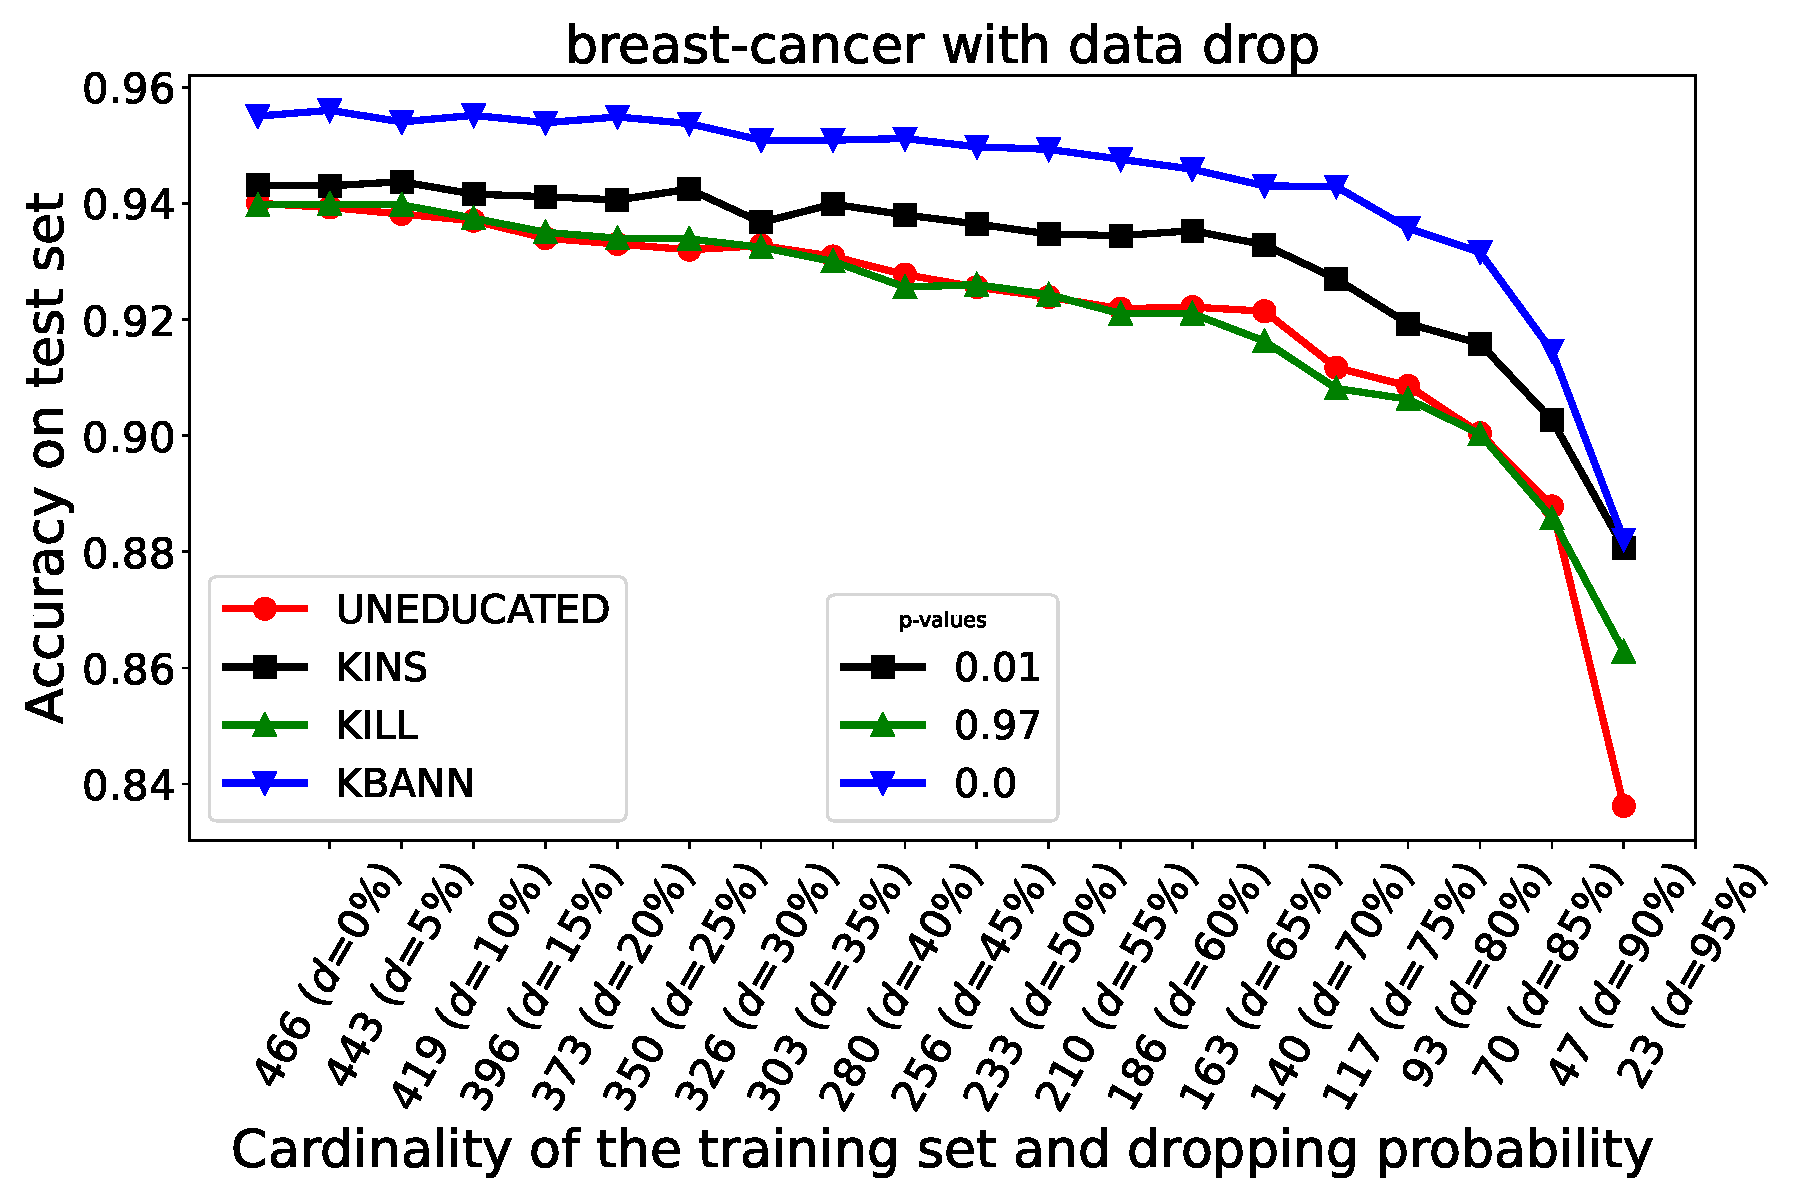
\includegraphics[width=\linewidth]{figures/drop/breast-cancer/uneducated-kins-kill-kbann-accuracy-average-curves}
	\end{subfigure}\hfil
	\begin{subfigure}{\cellsize}
		\caption{}
		\label{fig:psjgs-drop}
		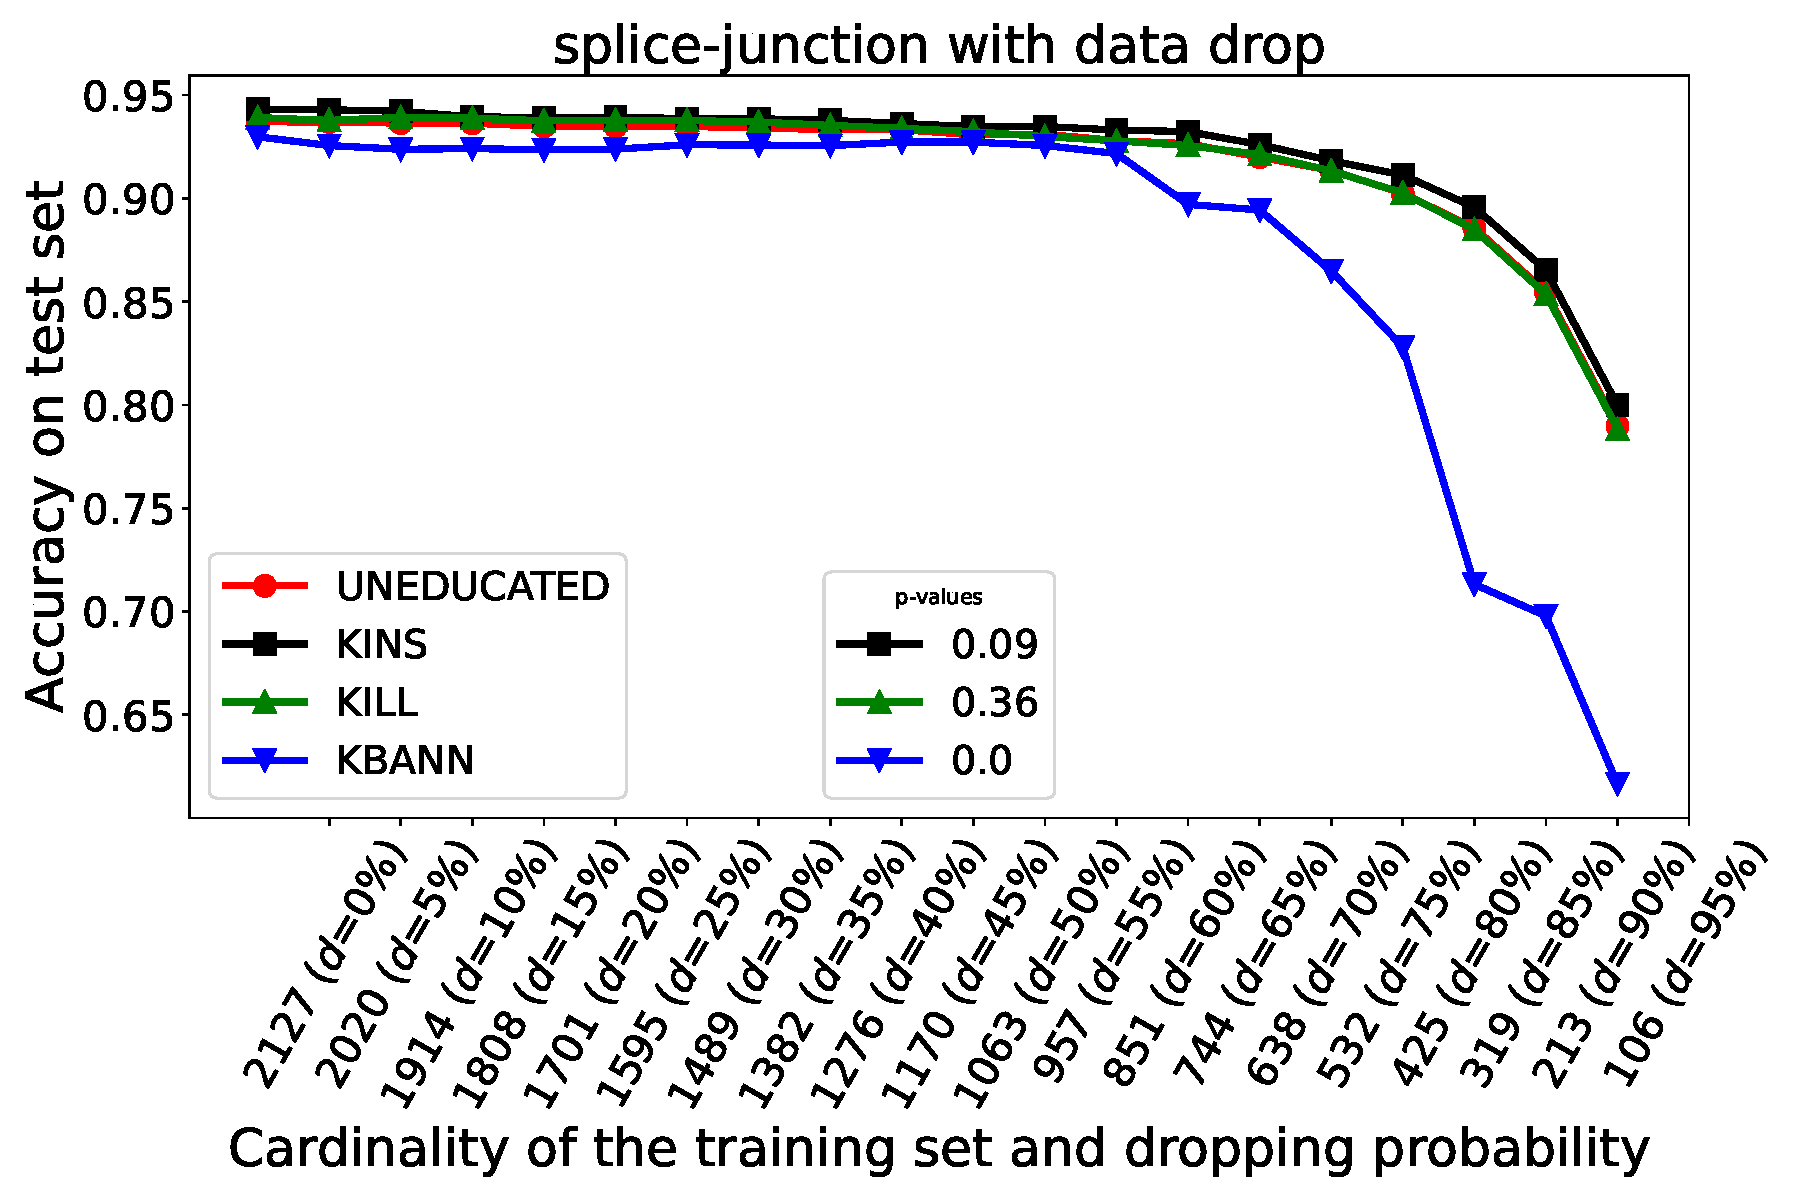
\includegraphics[width=\linewidth]{figures/drop/splice-junction/uneducated-kins-kill-kbann-accuracy-average-curves}
	\end{subfigure}\hfil
	\begin{subfigure}{\cellsize}
		\caption{}
		\label{fig:ci-drop}
		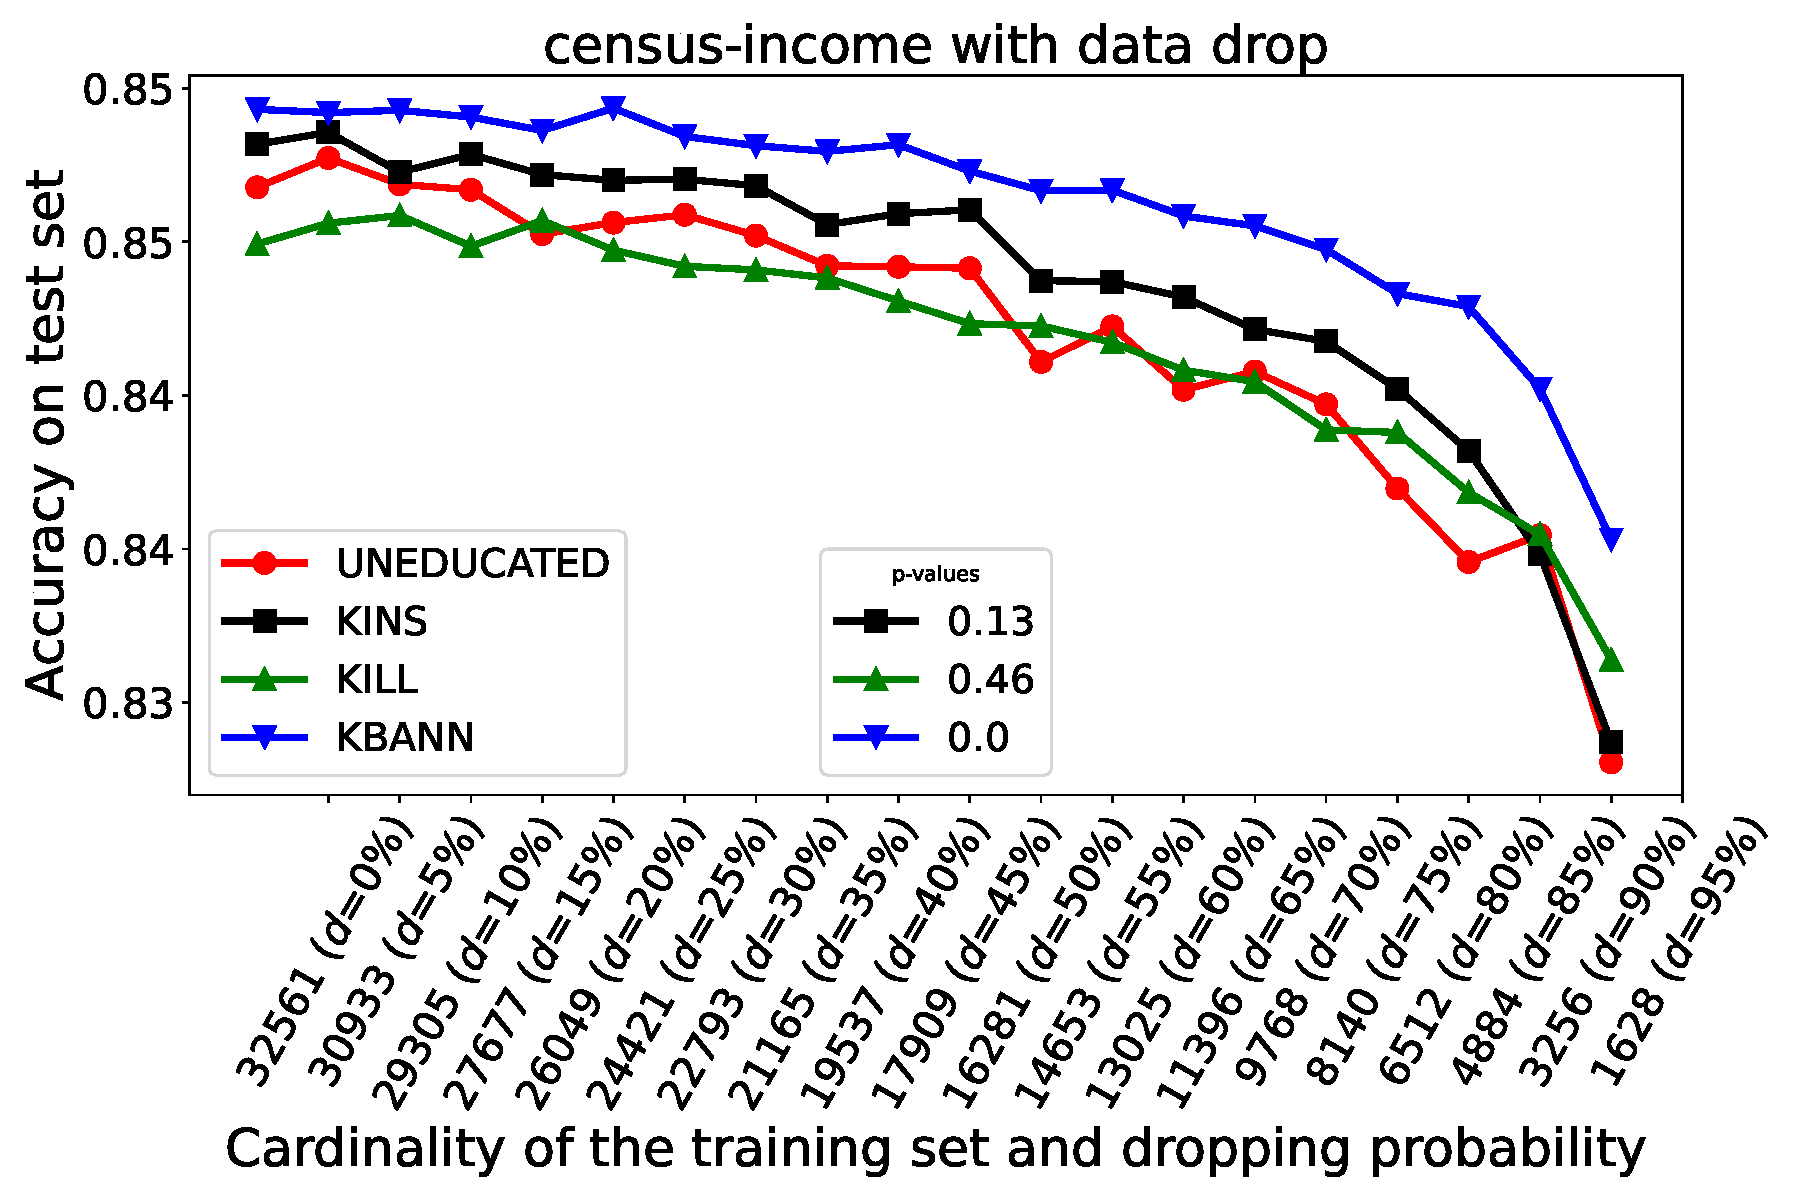
\includegraphics[width=\linewidth]{figures/drop/census-income/uneducated-kins-kill-kbann-accuracy-average-curves}
	\end{subfigure}

	\begin{subfigure}{\cellsize}
		\caption{}
		\label{fig:bcw-noise}
		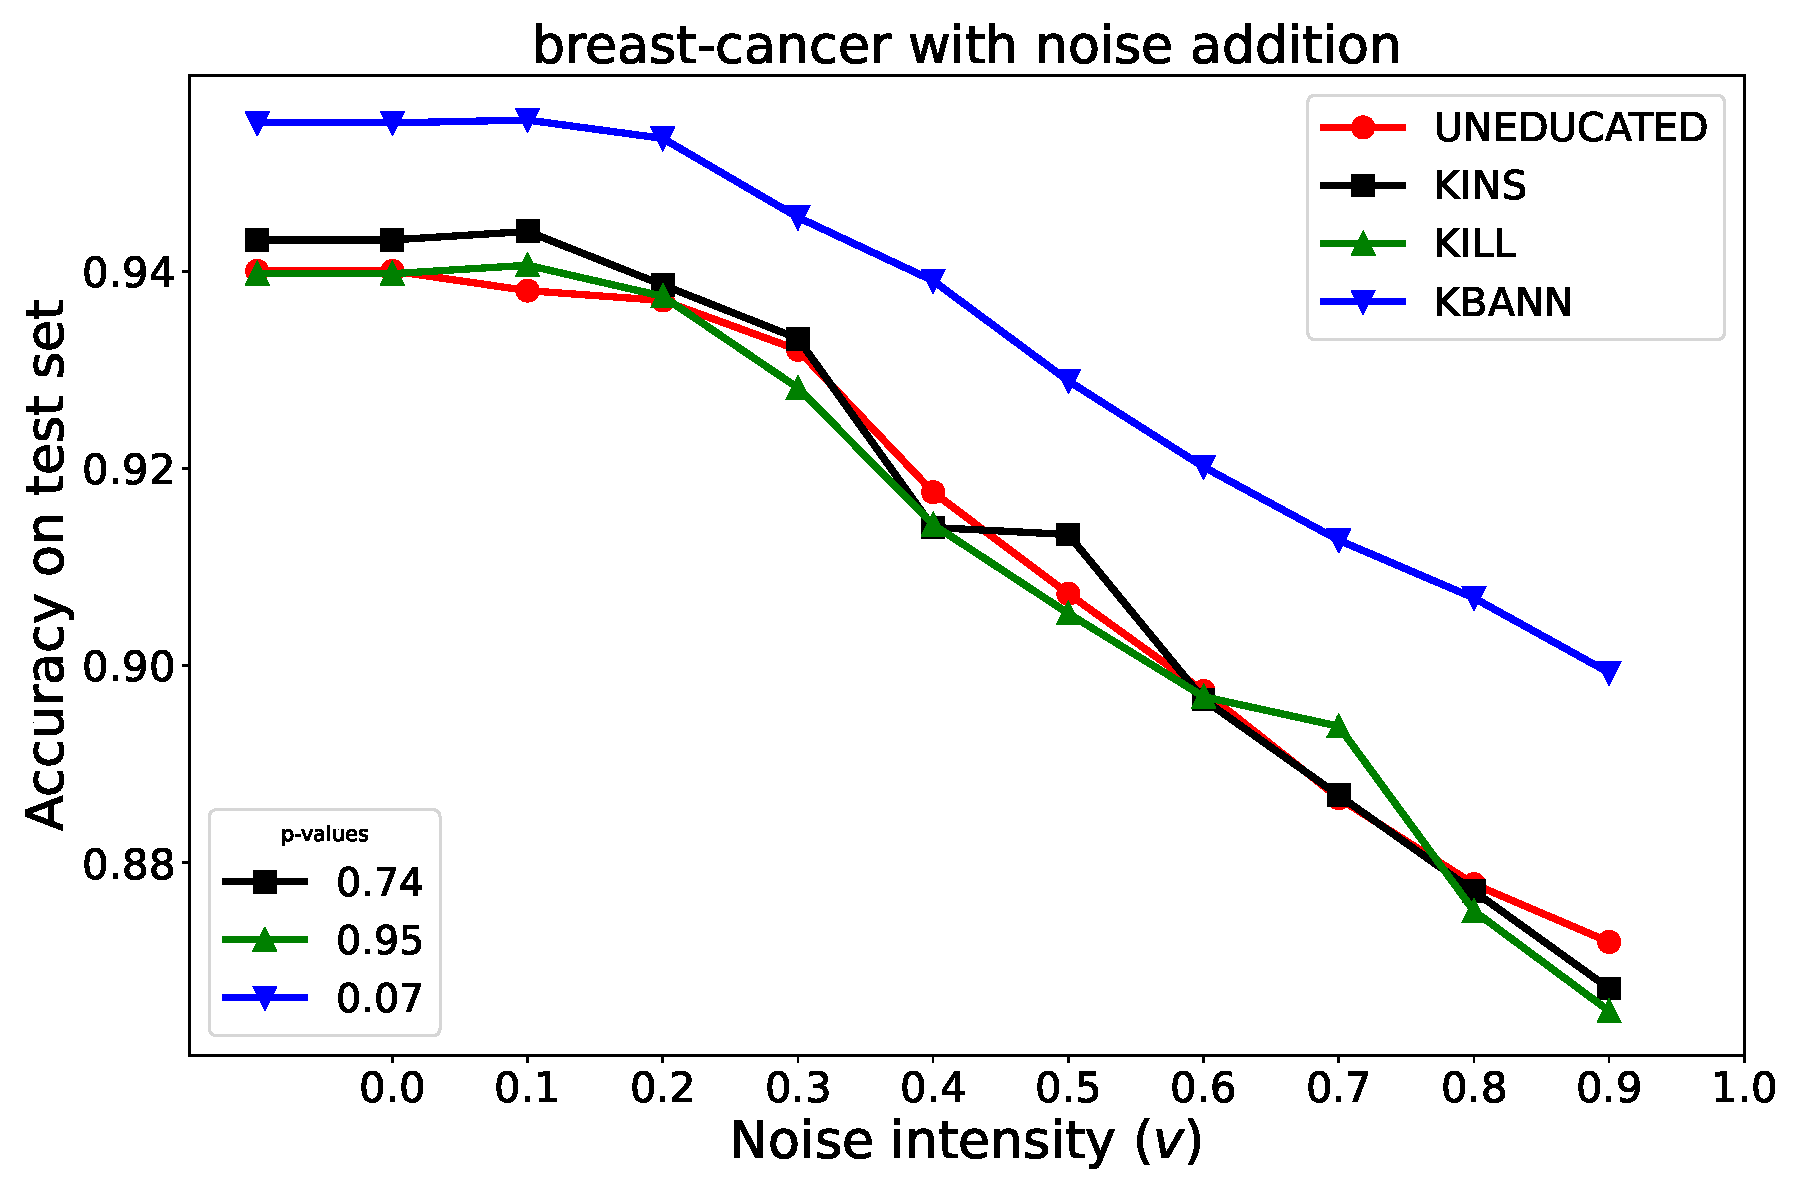
\includegraphics[width=\linewidth]{figures/noise/breast-cancer/uneducated-kins-kill-kbann-accuracy-average-curves}
	\end{subfigure}\hfil
	\begin{subfigure}{\cellsize}
		\caption{}
		\label{fig:psjgs-noise}
		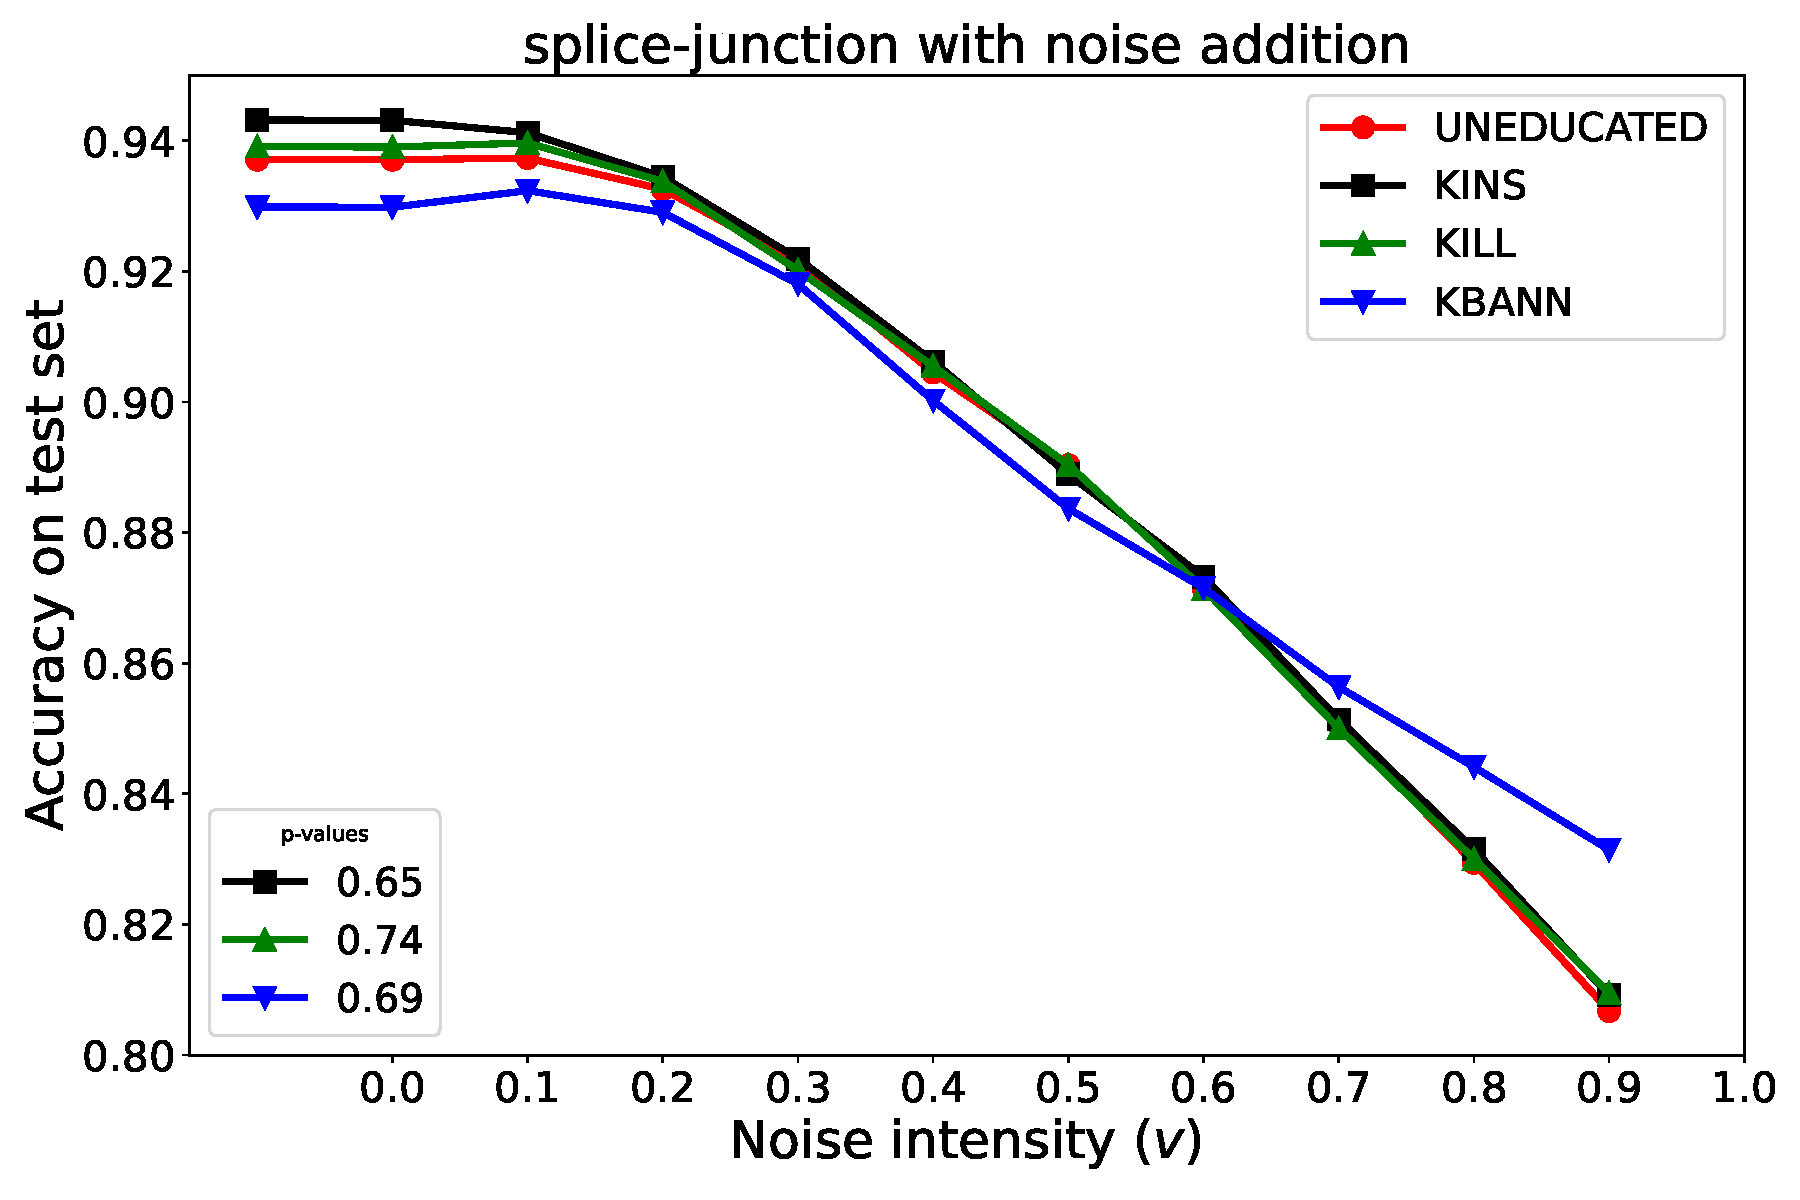
\includegraphics[width=\linewidth]{figures/noise/splice-junction/uneducated-kins-kill-kbann-accuracy-average-curves}
	\end{subfigure}\hfil
	\begin{subfigure}{\cellsize}
		\caption{}
		\label{fig:ci-noise}
		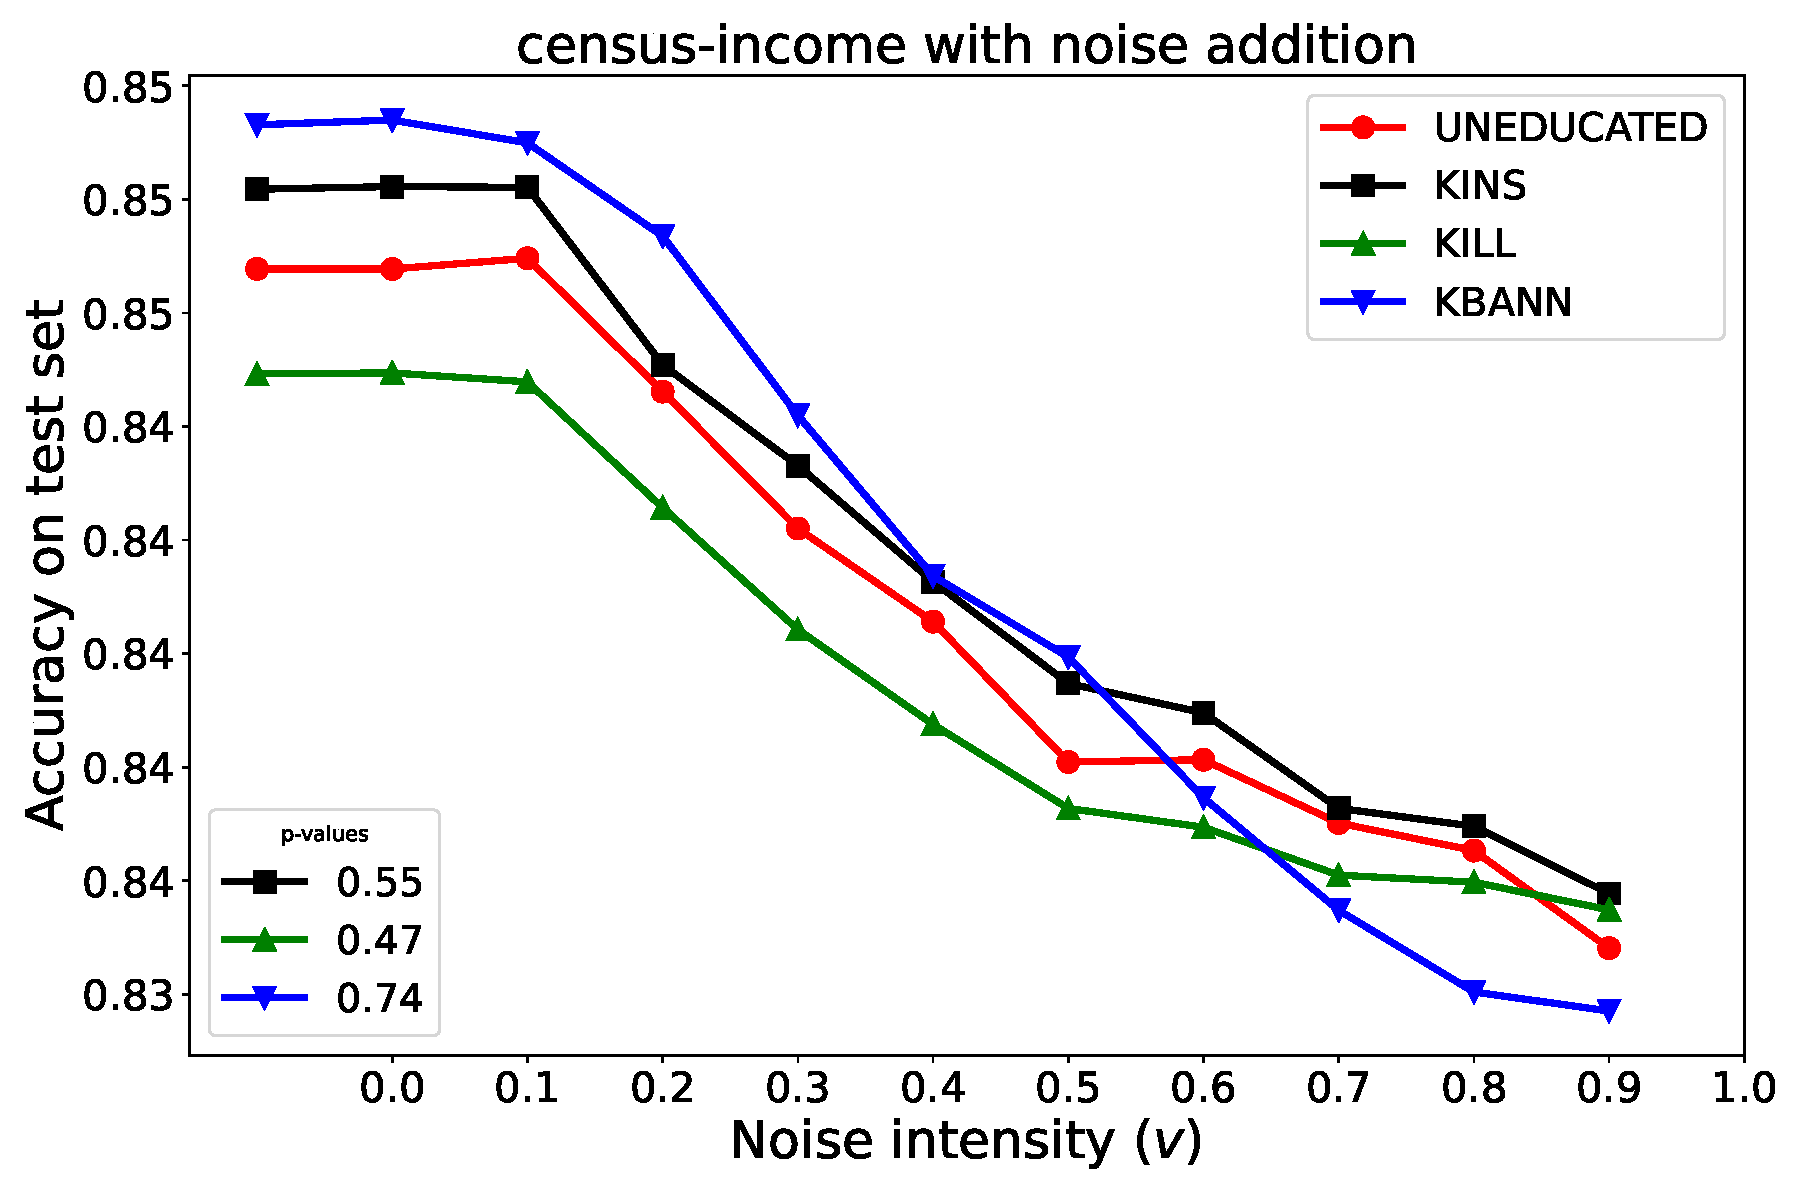
\includegraphics[width=\linewidth]{figures/noise/census-income/uneducated-kins-kill-kbann-accuracy-average-curves}
	\end{subfigure}

	\begin{subfigure}{\cellsize}
		\caption{}
		\label{fig:bcw-label}
		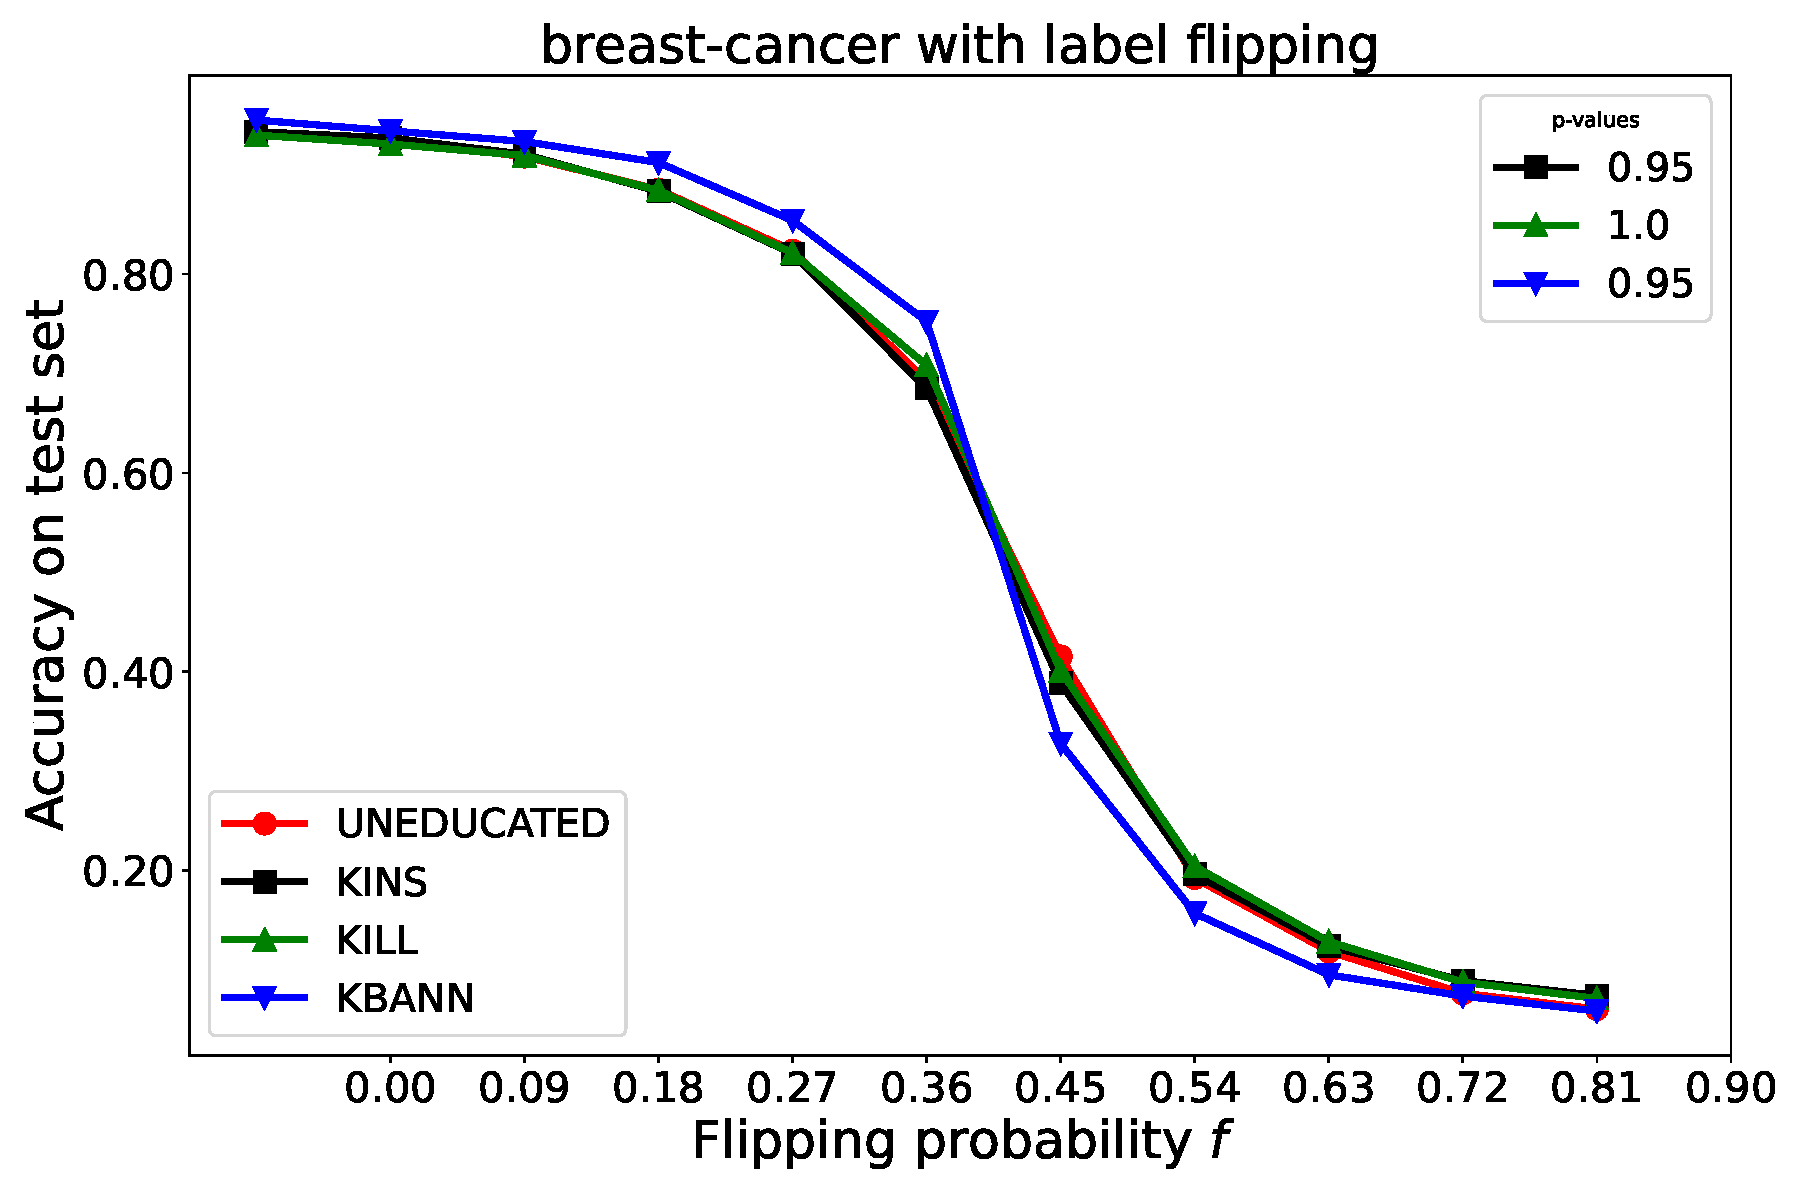
\includegraphics[width=\linewidth]{figures/label_flip/breast-cancer/uneducated-kins-kill-kbann-accuracy-average-curves}
	\end{subfigure}\hfil
	\begin{subfigure}{\cellsize}
		\caption{}
		\label{fig:psjgs-label}
		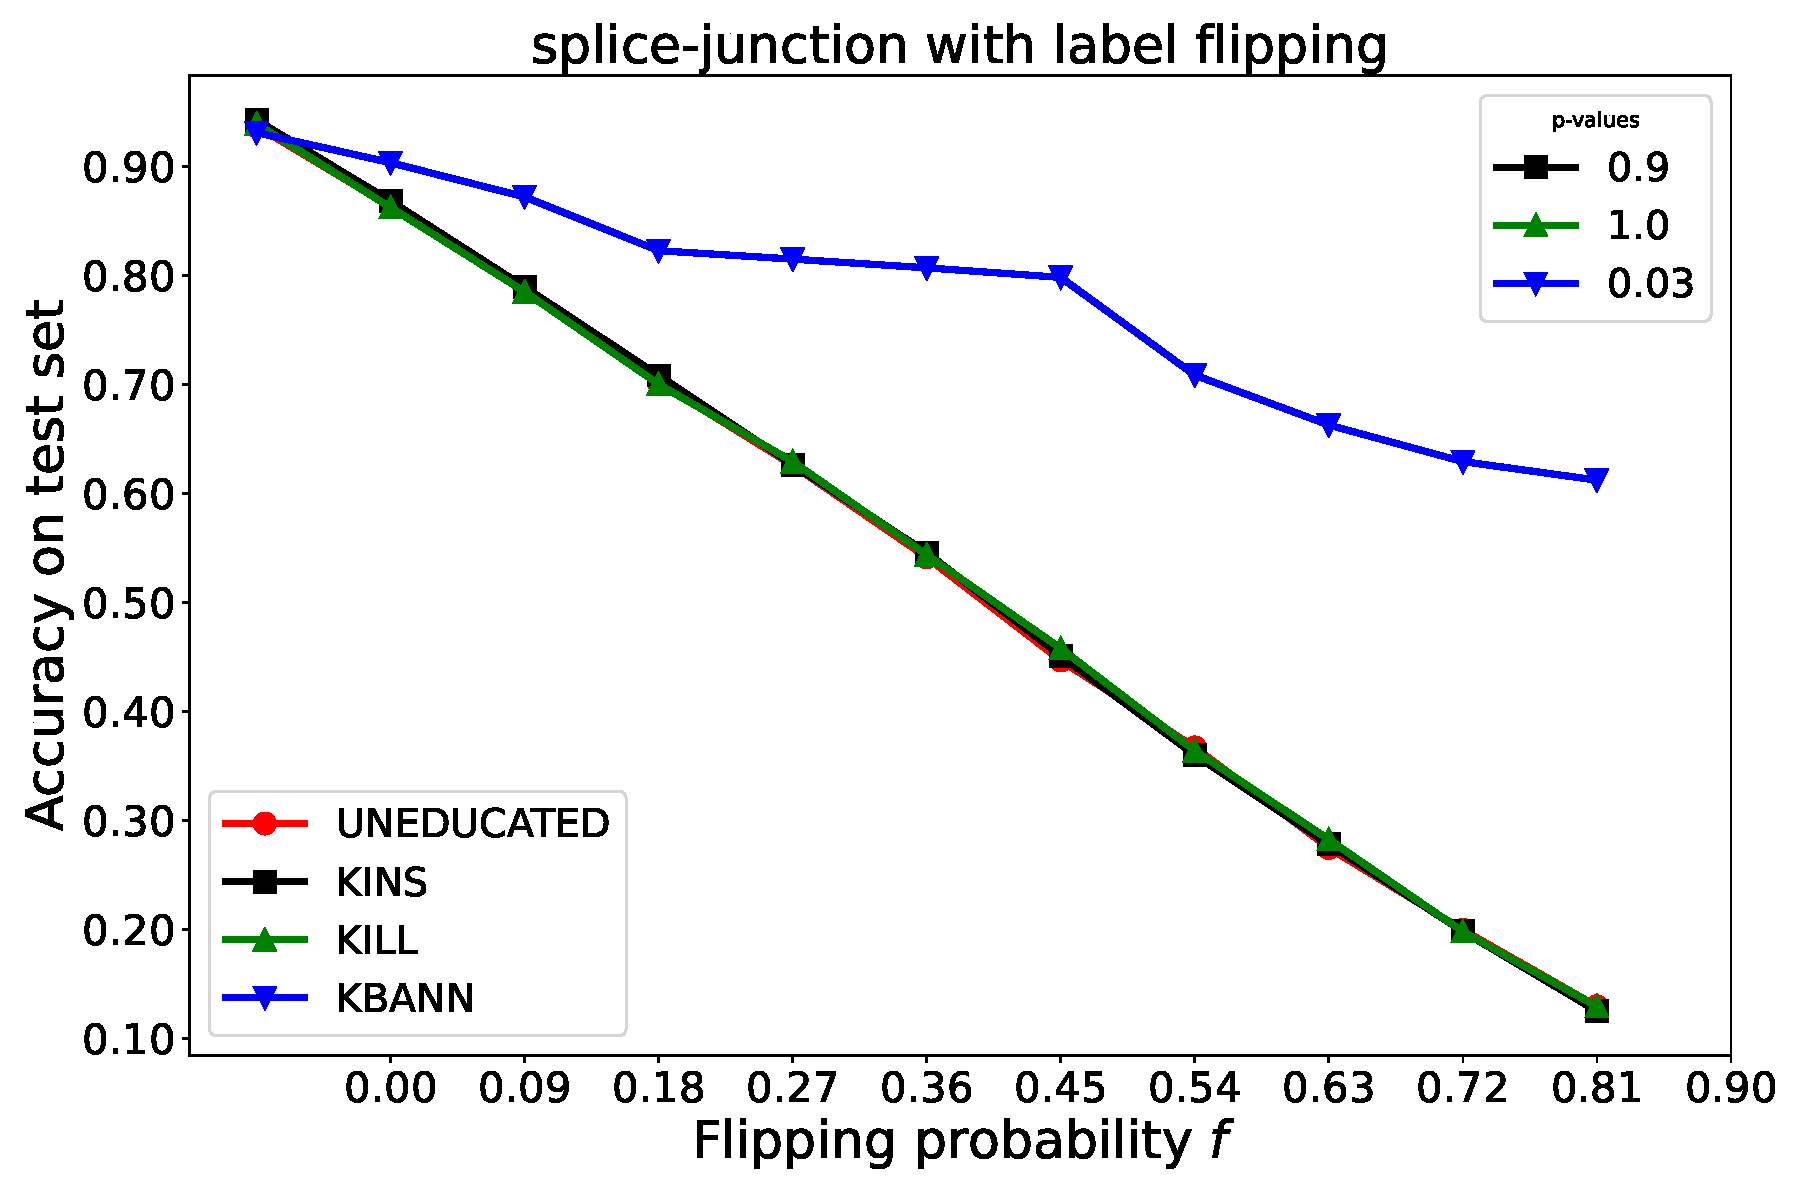
\includegraphics[width=\linewidth]{figures/label_flip/splice-junction/uneducated-kins-kill-kbann-accuracy-average-curves}
	\end{subfigure}\hfil
	\begin{subfigure}{\cellsize}
		\caption{}
		\label{fig:ci-label}
		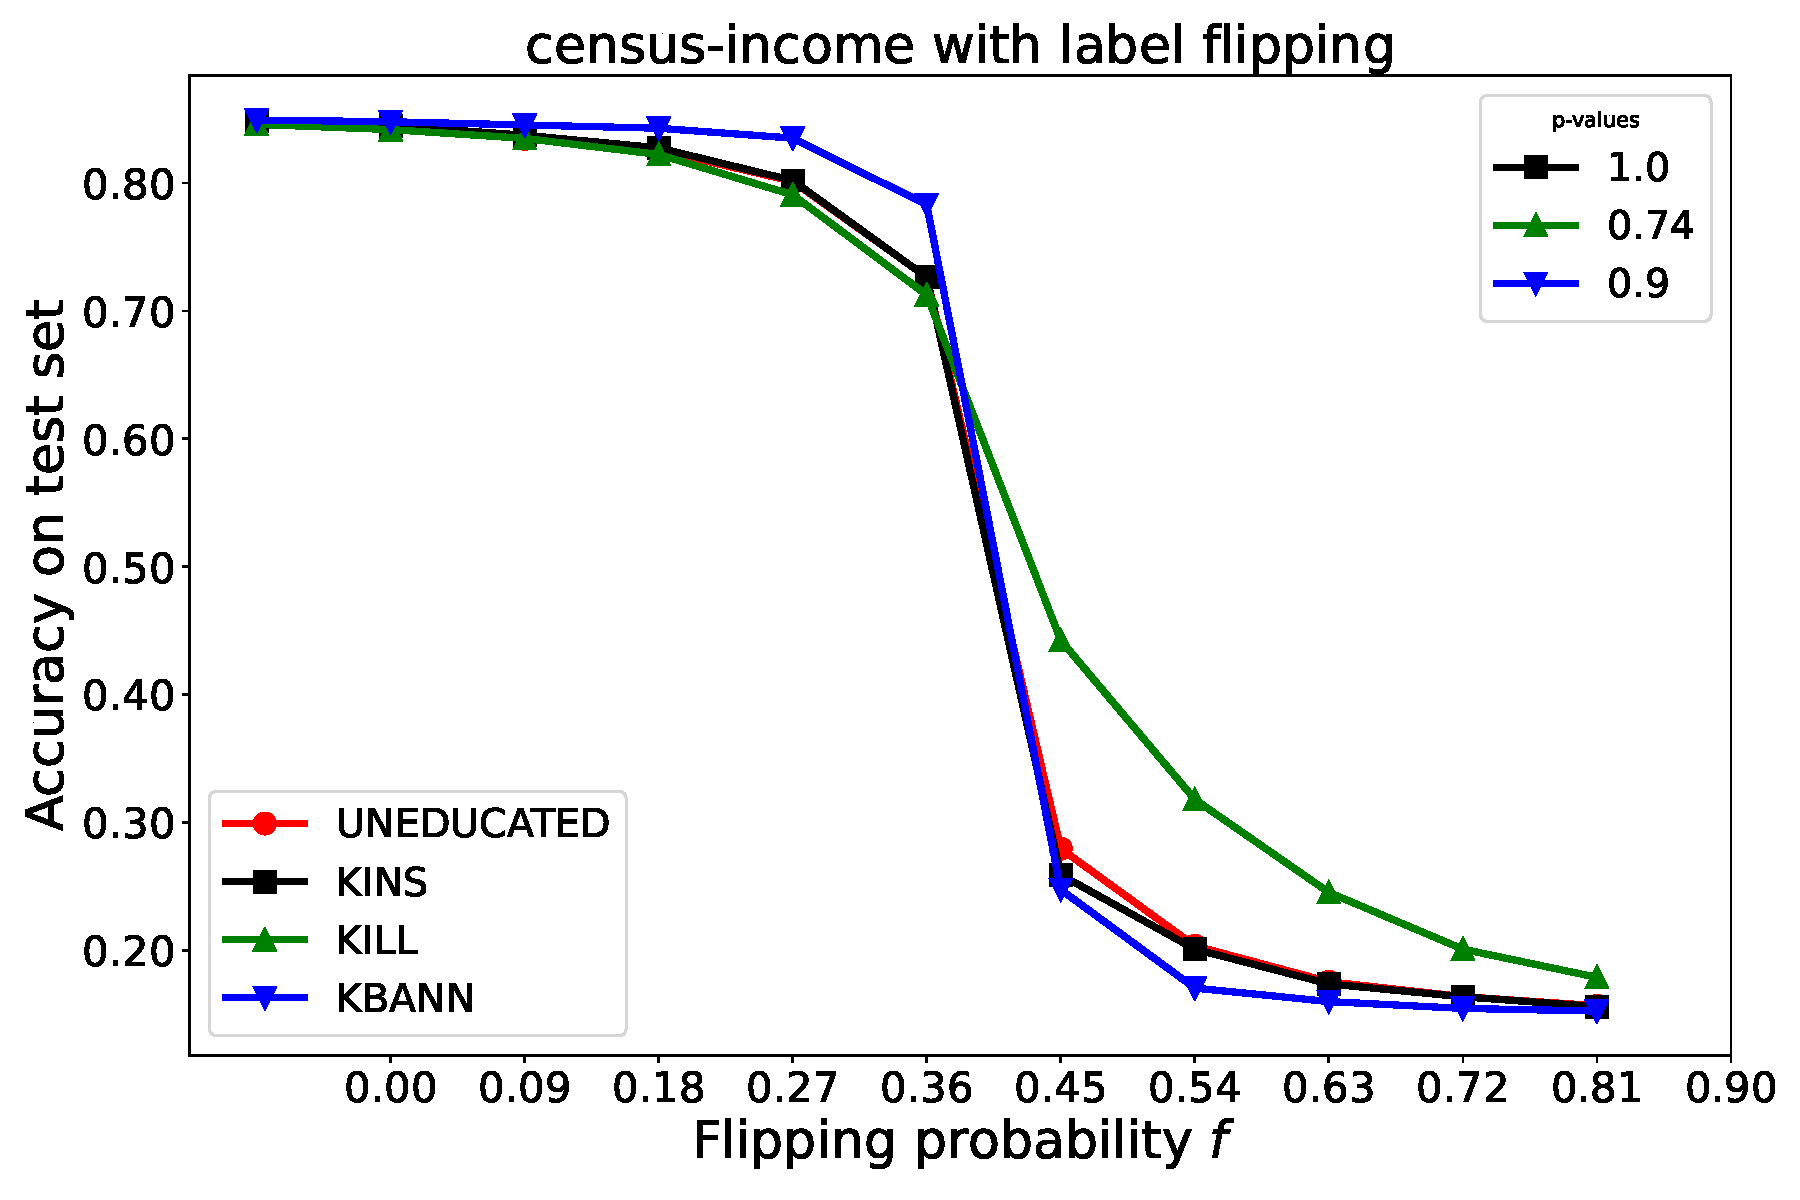
\includegraphics[width=\linewidth]{figures/label_flip/census-income/uneducated-kins-kill-kbann-accuracy-average-curves}
	\end{subfigure}
	\caption{Average accuracy over different datasets with different perturbation strategies}
	\label{fig:accuracy-results}
\end{figure*}
%
\note{TODO: generate again the figures because there is an issue with the x ticks labels}
%
% !TeX root = ../phd-thesis.tex
\begin{table}
    \centering
     \resizebox{\columnwidth}{!}{
         \begin{tabular}{l||rrr|rrr|rrr}
             \toprule
             \multirow{2}{*}{Dataset} &  \multicolumn{3}{c|}{$R_{N, D}(\mathcal{I})$ drop} &  \multicolumn{3}{c|}{$R_{N, D}(\mathcal{I})$ noise} &  \multicolumn{3}{c}{$R_{N, D}(\mathcal{I})$ flip}\\
             \cmidrule{2-10}
             & KINS &  KILL &  KBANN & KINS &  KILL &  KBANN & KINS &  KILL &  KBANN\\
             \midrule
             BCW    & \textbf{1.0493} & \textbf{1.0318} & \textbf{1.0382}  & 0.9960 & 0.9985 & \textbf{1.0109} & 0.9994 & \textbf{1.0184} & 0.9520\\
             PSJGS & \textbf{1.0045} & 0.9968 & 0.8425 & 0.9950 & 0.9984 & \textbf{1.0145} & 0.9962 &  \textbf{1.0026} & \textbf{1.6749} \\
             CI   &  0.9998 & \textbf{1.0039} & \textbf{1.0043} & 0.9992 & \textbf{1.0012} &  0.9965 & 0.9897 & \textbf{1.1703} & 0.9815 \\
             \bottomrule
         \end{tabular}
     }
    \caption[Robustness relative scores for drop, noise and label flip perturbations]{
        %
        Robustness relative scores $R_{N, D}(\mathcal{I})$ for the three perturbation strategies: drop, noise and label flip.
        %
        Bold numbers are the ones greater than 1 (i.e., the educated model is more robust than the uneducated one).
    }
    \label{tab:robustness}
\end{table}


%
This section presents the results of our experiments, focusing on the robustness of educated and uneducated predictors under different perturbation strategies.
%
To compare their performance, we use the \emph{Mann-Whitney U Test}~\cite{Mann-Whitney2010}, a non-parametric statistical test.
%
A p-value \(\geq 0.05\) indicates no significant difference between the average accuracy distributions, while a p-value \(< 0.05\) suggests otherwise.


\paragraph{Data Drop}
%
In the \emph{data drop} experiments (~\Cref{fig:bcw-drop,fig:psjgs-drop,fig:ci-drop}), \gls{KBANN} is the only predictor showing significant improvements compared to the uneducated model.
%
It performs better on the \gls{BCW} (\Cref{fig:bcw-drop}) and \gls{CI} (\Cref{fig:ci-drop}) datasets but exhibits a sharp decline on the \gls{PSJGS} dataset (\Cref{fig:psjgs-drop}) when 60\% of the data is removed (\(d = 0.6\)).
%
\gls{KINS} shows slightly better performance than the uneducated model, with a p-value of 0.01 on the \gls{BCW} dataset, indicating significant differences.
%
Overall, educated predictors improve robustness in 6 out of 9 experiments, as shown in \Cref{tab:robustness}.


\paragraph{Noise Addition}
%
The \emph{noise addition} experiments (\Cref{fig:bcw-noise,fig:psjgs-noise,fig:ci-noise}) reveal that \gls{SKI} mechanisms are more sensitive to noise than to missing data.
%
Predictors trained on noisy data show a rapid decline in accuracy, starting early in the perturbation process.
%
\gls{KBANN} outperforms other methods and the uneducated model on the \gls{BCW} dataset (\Cref{fig:bcw-noise}) but performs poorly on the \gls{CI} (\Cref{fig:ci-noise}) and \gls{PSJGS} (\Cref{fig:psjgs-noise}) datasets.
%
Interestingly, \gls{KINS} performs worse than \gls{KBANN}, likely due to its trainable modules being more prone to overfitting noisy data.
%
\gls{KILL} shows similar or worse performance compared to the uneducated model, suggesting that its penalty-based approach does not effectively handle noise perturbations.


\paragraph{Label Flipping}
%
In the \emph{label flipping} experiments (\Cref{fig:bcw-label,fig:psjgs-label,fig:ci-label}), predictors exhibit similar behavior on the \gls{BCW} (\Cref{fig:bcw-label}) and \gls{CI} (\Cref{fig:ci-label}) datasets, with no significant differences (p-values close to 1).
%
Performance degrades rapidly when more than 54\% of labels are flipped (\(f = 0.54\)).
%
On the \gls{PSJGS} dataset (\Cref{fig:psjgs-label}), \gls{KBANN} retains nearly 70\% accuracy even at the highest flipping probability (\(f = 0.9\)), outperforming other models, which drop to 20\%.
%
This highlights \gls{KBANN}'s strong adherence to injected knowledge, which mitigates the impact of flipped labels.
%
\gls{KILL} demonstrates good robustness across all datasets, likely due to its loss manipulation strategy, which de-emphasizes corrupted labels during training.


\paragraph{Discussion and Take-Home Message}
%
The experiments show that \gls{SKI} methods are most effective in handling missing data, leveraging integrated knowledge to compensate for data scarcity.
%
However, their robustness to noise perturbations is limited, with no significant improvements observed.
%
For label flipping, \gls{KILL} performs well due to its penalty-based approach, while \gls{KBANN} excels on the \gls{PSJGS} dataset due to its strong reliance on injected knowledge.
%
In summary:
%
\begin{enumerate}
    \item \gls{SKI} methods enhance robustness under data scarcity by utilizing integrated knowledge.
    %
    \item Loss-manipulating techniques like \gls{KILL} better tolerate label corruption by reducing the impact of flawed labels.
    %
    \item Structuring-based methods like \gls{KBANN} are more robust than trainable approaches like \gls{KINS}, as they preserve the integrity of injected knowledge.
\end{enumerate}
%
These findings emphasize the importance of selecting appropriate \gls{SKI} methods based on the type of perturbation and dataset characteristics.
%! Author = matteomagnini
%! Date = 05/03/25

%----------------------------------------------------------------------------------------
\chapter[Fairness through SKI]{Fairness through \gls{SKI}}
\label{ch:fairness-through-ski}
\minitoc
%----------------------------------------------------------------------------------------

\Gls{AI} has transformed various aspects of modern society.
%
With recent groundbreaking advancements, its applications are expected to grow exponentially.
%
However, the issue of fairness has become a significant concern.
%
When \gls{AI} systems are deployed without adequate safeguards, they risk perpetuating or amplifying existing social biases.
%
For example, a recruitment system trained on historical data dominated by male hires may discriminate against female applicants, reinforcing gender bias~\cite{kochling2020discriminated}.
%
To address such challenges, numerous techniques have been developed to mitigate bias in \gls{AI}.
%
Among these, regularization-based fairness techniques have gained prominence for balancing fairness and predictive performance.
%
Regularization, initially introduced to prevent overfitting, involves adding a penalty term to the loss function during training.
%
Recently, it has been extended to promote fairness by incorporating penalties derived from fairness constraints~\cite{DBLP:conf/icdm/KamishimaAS11}.
%
These methods aim to reduce the dependence of predictions on sensitive attributes, such as gender, making them effective for bias mitigation during optimization steps like \gls{SGD} in \gls{ML} algorithms.
%

\section{Background}\label{sec:fairness-background}
%
We provide a brief but comprehensive overview of fairness in \gls{ML} to understand our contributions without delving into the extensive literature on the topic.
%
The section is organised as follows.
%
In \Cref{subsec:fairness-in-ai}, we discussed the motivations for fairness in \gls{ML}.
%
In \Cref{subsec:fairness-metrics}, we introduce common group fairness metrics used in the literature, along with some of their limitations that motivate the development novel metrics.
%
We conclude the background section with a presentation of related works in \Cref{subsec:fairness-ski}.
%
Finally, in \Cref{sec:fauci}, we present our contributions to fairness in \gls{ML}.


\subsection{Fairness metrics}\label{subsec:fairness-metrics}
%
We introduce three of the most popular \emph{group fairness} metrics used in \gls{ML} to evaluate the fairness of models.
%
Despite being used in many works, these metrics suffer certain limitations, such as being applicable only to binary classification tasks or requiring specific types of sensitive attributes.
%
In particular, all three metrics -- as defined below in their first formulation -- can support only binary or categorical sensitive attributes, i.e., \( A \in \{0, 1\} \) or \( A \in \{a_1, a_2, \ldots, a_n\} \) for some \( n \in \mathbb{N} \).
%
Moreover, the metrics do not take into account the option to weight groups differently.
%
This possibility could be useful in scenarios of highly unbalanced groups.
%
These limitations are the driver that will lead to the development of novel fairness metrics in \Cref{sec:fauci}.


\Glsfull{DP} is a fairness metric, also referred to as \emph{statistical parity}, that evaluates whether the predictions of a \gls{ML} model are independent of a given protected attribute.
%
This implies that the values of the sensitive feature do not influence the model's output~\cite{DBLP:conf/innovations/DworkHPRZ12}.
%
\Gls{DP} compares the distribution of the model's predictions with the distribution of predictions conditioned on the values of the sensitive attribute.
%
For a binary classifier \( h \) and a discrete sensitive attribute \( A \), \gls{DP} is mathematically defined as:
%
\begin{equation}
    \label{eq:dp}
    \text{DP}_{h,A}(X) = \sum_{a \in A} \left| \mathbb{E}[h(X) \mid A = a] - \mathbb{E}[h(X)] \right|,
\end{equation}
%
where \( X \) represents the test data, \( A \) denotes the sensitive attribute, \( a \) is a specific value of \( A \), \( \mathbb{E} \) is the expectation operator, and \( \left| \cdot \right| \) is the absolute value.
%
A model \( h \) satisfies DP if the computed value is below a predefined bias threshold \( \epsilon \), commonly set to \( 0.01 \).
%
\Gls{DP} is particularly useful in applications such as loan approvals, where it ensures that approval rates are consistent across demographic groups, thereby mitigating discrimination.


\Glsfull{DI} quantifies the disproportionate effect of a classifier on individuals based on a sensitive attribute~\cite{DBLP:conf/kdd/FeldmanFMSV15}.
%
For binary classification tasks and binary sensitive attributes, \gls{DI} is initially defined as the ratio:
%
\begin{equation}
    \label{eq:di_unbounded}
    \text{di}_{h,A}(X) = \frac{\mathbb{E}[h(X) \mid A = 1]}{\mathbb{E}[h(X) \mid A = 0]}.
\end{equation}
%
To ensure bounded values within \([0, 1]\), DI is commonly standardized using the function \( \eta(x) = \min\{x, x^{-1}\} \), resulting in:
%
\begin{equation}
    \label{eq:di}
    \text{DI}_{h,A}(X) = \eta(\text{di}_{h,A}(X)).
\end{equation}
%
Values of \gls{DI} above \( 0.8 \) are generally considered acceptable, with lower values indicating higher fairness violations.
%
In scenarios requiring positive scores, \( 1 - \text{DI} \) may be reported, such as during the training of neural networks.
%
\Gls{DI} is applicable in contexts like loan approvals, where it helps identify disproportionate denial rates affecting specific demographic groups.


\Glsfull{EO} measures the extent to which a classifier predicts a given class equally across all values of a sensitive attribute~\cite{DBLP:conf/nips/HardtPNS16}.
%
For binary classification (\( Y \in \{0, 1\} \)) and a categorical sensitive attribute \( A \), \gls{EO} is defined as:
%
\begin{equation}
    \label{eq:eo}
    \text{EO}_{h,A}(X) = \sum_{(a, y) \in A \times Y} \text{eo}_{h,A}(X, a, y),
\end{equation}
%
where \( Y \) represents the ground truth, and \( \text{eo}_{h,A}(X, a, y) \) is given by:
%
\begin{equation}
    \label{eq:eo_partial}
    \text{eo}_{h,A}(X, a, y) = \left| \mathbb{E}[h(X) \mid A = a, Y = y] - \mathbb{E}[h(X) \mid Y = y] \right|.
\end{equation}
%
Similar to \gls{DP}, a classifier is considered fair if its \gls{EO} value is below a predefined bias threshold \( \epsilon \).
%
\Gls{EO} is valuable in applications like loan approvals, where it identifies disparities in approval rates that may favor specific demographic groups.



\subsection{Fairness and SKI}\label{subsec:fairness-ski}
%
How promoting fairness in \gls{ML} models can be achieved through \gls{SKI} methods?
%
It is definitively possible if we keep our attention on \emph{in-processing} methods, which enforce fairness during model training, and on \emph{group fairness} metrics, which measure the extent to which a model is biased against certain groups.
%
Indeed, the process of including fairness constraints in the training loss can be seen as a form of regularization, similar to how \gls{SKI} methods incorporate constraints into the optimization process.
%
The knowledge that usually \gls{SKI} methods leverage is about the \gls{ML} task at hand (e.g., classification, regression) and the relationships between features and target variables, most commonly in order to improve generalization and interpretability.
%
In the context of fairness, this knowledge includes fairness-related constraints -- still consisting in relationships between features and target variables -- that are used to ensure that the model does not discriminate against certain groups based on \emph{sensitive attributes}.
%
Instead of using logical operators between expressions involving features and constants (see for example \Cref{subsec:kill-validation}), fairness metrics are directly involved.
%
Still, a knowledge of this kind can be expressed with a symbolic formalism, and therefore the whole process can be seen as a form of \gls{SKI} according \Cref{def:ski}.


\subsubsection{Related Works}
%
This section highlights key contributions in the literature on \emph{in-processing} fairness methods applied to \emph{group fairness} metrics.
%
Among these, regularization-based approaches are widely used to mitigate bias in \gls{AI} systems.
%
These methods incorporate fairness constraints directly into the training process by modifying the loss function.
%
The regularization term penalizes unfair predictions, with variations in its definition leading to differences in effectiveness, efficiency, and scalability.
%

\paragraph{\Glsfull{KDE}}
\label{par:kde-fairness}
%
\Gls{KDE}~\cite{DBLP:conf/nips/ChoHS20} introduces a non-parametric fairness regularization approach using kernel density estimation.
%
The method estimates probabilities such as \( \mathbb{P}[h(X) = y^+ \mid S = s] \) and \( \mathbb{P}[h(X) = y^+ \mid S = s, Y = y] \) as differentiable functions with respect to model parameters.
%
This enables direct optimization through gradient-based methods for fairness metrics like \gls{DP} and \gls{EO}.
%
Instead of using the final model output \( h(X) \), the method relies on an internal value \( \tilde{Y} \in [0, 1] \), representing the probability of an instance belonging to the positive class.
%
The final output \( h(X) \) is assigned to the positive class if \( \tilde{y}_i \geq \tau \), where \( \tau \) is a predefined threshold.
%
For \gls{DP}, the probability density function is estimated using a Gaussian kernel:
%
\begin{equation}
    \label{eq:kde-fairness}
    f_k(\tilde{y}) = \frac{1}{\sqrt{2\pi}} \exp\left(-\frac{\tilde{y}^2}{2}\right).
\end{equation}
%
The probability estimate is obtained by integrating over the region \( \tilde{y} \geq \tau \):
%
\begin{equation}
    \label{eq:kde-fairness-probability}
    \mathbb{P}[h(X) = y^+ \mid S = s] = \int_{\tau}^{\infty} \frac{1}{|I_s|b} \sum_{i \in I_s} f_k\left(\frac{\tilde{y} - \tilde{y}_i}{b}\right) \, d\tilde{y},
\end{equation}
%
where \( I_s \) is the set of instances with sensitive attribute \( S = s \), \( \tilde{y}_i \) is the internal model value for instance \( i \), and \( b \) is the bandwidth parameter.
%
To achieve \gls{DP}, the difference in probabilities across sensitive groups is minimized:
%
\begin{equation}
    \label{eq:kde-fairness-regularizer}
    R_{\text{KDE}}(h, D_{\text{train}}, b) \approx \sum_{s \in S} H_\delta\left(\mathbb{P}[h(X) = y^+ \mid S = s] - \mathbb{P}[h(X) = y^+]\right),
\end{equation}
%
where \( H_\delta(\cdot) \) is the Huber function, a smooth approximation of the absolute value operator~\cite{10.1214/aoms/1177703732}.
%

\paragraph{\Glsfull{GDP}}
\label{par:gdp-fairness}
%
\Gls{GDP}~\cite{DBLP:conf/iclr/JiangHFYMH22} extends \gls{DP} to continuous sensitive attributes while ensuring differentiability.
%
It measures the deviation between the conditional probability \( \mathbb{P}[h(X) = y^+ \mid S = s] \) and the marginal probability \( \mathbb{P}[h(X) = y^+] \), weighted by the probability density function of \( S \).
%
Two estimation methods are proposed: histogram-based and kernel-based.
%
The histogram-based method partitions the range of \( S \) into non-overlapping bins \( B = \{B_1, \ldots, B_{|B|}\} \) of equal width \( b \).
%
Within each bin \( B_i \), the local and global prediction averages are computed as:
%
\begin{equation}
    \label{eq:gdp-averages}
    \text{avg}_{\text{local}}(B_i, h) = \sum_{j \in I_{B_i}} \tilde{y}_j, \quad \text{avg}_{\text{global}}(h, D_{\text{train}}) = \frac{1}{|D_{\text{train}}|} \sum_{n=1}^{|D_{\text{train}}|} \tilde{y}_n,
\end{equation}
%
where \( I_{B_i} \) contains the indices of instances in bin \( B_i \).
%
The fairness regulariser is defined as:
%
\begin{equation}
    \label{eq:gdp-regulariser}
    R_{\text{hist-GDP}}(h, D_{\text{train}}, b) = \sum_{i=1}^{b} \left(\text{avg}_{\text{local}}(B_i, h) - \text{avg}_{\text{global}}(h, D_{\text{train}})\right) \cdot \mathbb{P}[S \in B_i].
\end{equation}
%
Kernel-based estimation provides smoother results by assigning soft group memberships using a kernel function \( K(\cdot) \), avoiding discontinuities at bin boundaries.
%

\paragraph{\Glsfull{FNNC}}
\label{par:fnnc-fairness}
%
\Gls{FNNC}~\cite{DBLP:conf/ijcai/ManishaG20} formulates fairness as a constrained optimization problem.
%
The goal is to minimize predictive performance loss subject to a fairness constraint.
%
For \gls{DP}, the problem is defined as:
%
\begin{equation}
    \label{eq:fnnc-fairness}
    h^\ast = \arg\min_{h \in H} L(h, D_{\text{train}}) \quad \text{s.t.} \quad \mathbb{P}[h(X) = y^+ \mid S = s] - \mathbb{P}[h(X) = y^+ \mid S \neq s] \leq \epsilon,
\end{equation}
%
where \( \epsilon \) is a predefined fairness threshold.
%
The fairness constraint is integrated into the loss function using the Lagrangian multiplier method:
%
\begin{equation}
    \label{eq:fnnc-fairness-regularizer}
    R_{\text{FNNC}}(h, D_{\text{train}}) = \mathbb{P}[h(X) = y^+ \mid S = s] - \mathbb{P}[h(X) = y^+ \mid S \neq s] - \epsilon.
\end{equation}
%
Optimization is performed using a two-step \gls{SGD} procedure, alternating between minimizing model parameters and maximizing Lagrangian multipliers.
%

\paragraph{\Glsfull{NSIF}}
\label{par:ltn-fairness}
%
\Gls{NSIF}~\cite{DBLP:conf/aaaiss/WagnerG21} leverages the \gls{LTN} framework to enforce fairness constraints.
%
Fairness constraints are expressed as formal logic rules, which influence the training of \glspl{NN}.
%
The method validates its effectiveness using \gls{DP} and \gls{DI} metrics for categorical sensitive attributes.
%
Although not regularization-based, \gls{NSIF} provides a unique approach to fairness through symbolic reasoning.


\section[Fairness under constraints injection]{\Glsentrylong{FaUCI}}\label{sec:fauci}
%
In this section, we present the contribution of the work ``Enforcing Fairness via Constraint Injection with FaUCI''~\cite{DBLP:conf/aequitas/MagniniCCO24}, presented at the 2nd AEQUITAS workshop on fairness and bias in \gls{AI} 2024.
%
The work introduces two distinct contributions: the introduction of novel fairness metrics -- more precisely the extensions of \gls{DP}, \gls{DI}, and \gls{EO} to categorical and continuous sensitive attributes -- and the development of a novel fairness regularization method, called \gls{FaUCI}, which injects fairness constraints into the training loss of a model.


\subsection{Novel fairness metrics}\label{subsec:novel-fairness-metrics}
%
This section introduces weighted and generalized variants of fairness metrics to support both categorical and continuous sensitive attributes.
%
These extensions aim to generalize fairness metrics beyond binary data, enabling their application to real-world datasets.
%
For instance, they allow prioritizing fairness for underrepresented groups, such as specific ethnicities, when more than two groups exist.
%
We focus on three metrics: \gls{DP}, \gls{DI}, and \gls{EO}, and propose their weighted and generalized formulations.


\paragraph{Weighted and Generalized Demographic Parity}
%
\Gls{DP} evaluates whether the predictions of a model are independent of a sensitive attribute.
%
For binary classification, the values \( \mathbb{E}[h(X) \mid A = a] \) and \( \mathbb{E}[h(X)] \) from \Cref{eq:dp} are bounded within \([0, 1]\).
%
The maximum theoretical value of \gls{DP} depends on the number of possible values of the sensitive attribute \( A \), i.e., \( 0 \leq \text{DP} \leq |A| \).
%
This variability makes comparisons across datasets challenging.
%
To address this, we propose two variants: \glsfull{WDP} and \glsfull{GDP}.


\Gls{WDP} is defined as:
%
\begin{equation}
    \label{eq:wdp}
    \text{WDP}_{h,A}(X) = \sum_{a \in A} \left| \mathbb{E}[h(X) \mid A = a] - \mathbb{E}[h(X)] \right| \cdot w_a,
\end{equation}
%
where \( w_a \) represents the weight of the \( a \)-th value of \( A \), and \( \sum_{a \in A} w_a = 1 \).
%
Weights can be chosen based on the distribution of \( A \) or set equally to avoid bias towards frequent values.


\Gls{GDP} extends \gls{DP} to continuous sensitive attributes:
%
\begin{equation}
    \label{eq:gdp}
    \text{GDP}_{h,A}(X) = \int_{l}^{u} \left| \mathbb{E}[h(X) \mid A = a] - \mathbb{E}[h(X)] \right| \cdot w_a \, da,
\end{equation}
%
where \( l \) and \( u \) are the minimum and maximum values of \( A \), and \( w_a \) is a user-defined weight function satisfying \( \int_{l}^{u} w_a \, da = 1 \).
%
The definition of the \gls{GDP} has been already introduced in a recent work~\cite{DBLP:conf/iclr/JiangHFYMH22}.
%
It is the only metric among the ones presented in this section that was already existing in the literature.


\paragraph{Weighted and Generalized Disparate Impact}
%
\Gls{DI} quantifies the disproportionate effect of a classifier on groups defined by a sensitive attribute.
%
For categorical attributes, we define \glsfull{WDI} as:
%
\begin{equation}
    \label{eq:wdi}
    \text{WDI}_{h,A}(X) = \sum_{a \in A} \eta \left( \frac{\mathbb{E}[h(X) \mid A = a]}{\mathbb{E}[h(X) \mid A \neq a]} \right) \cdot w_a,
\end{equation}
%
where \( \eta(x) = \min\{x, x^{-1}\} \) ensures bounded values within \([0, 1]\).


For continuous attributes, \glsfull{GDI} is defined as:
%
\begin{equation}
    \label{eq:gdi}
    \text{GDI}_{h,A}(X) = \int_{l}^{u} \eta \left( \frac{\mathbb{E}[h(X) \mid A = a]}{\mathbb{E}[h(X) \mid A \neq a]} \right) \cdot w_a \, da.
\end{equation}


\paragraph{Weighted and Generalized Equalized Odds}
%
\Gls{EO} measures whether a classifier predicts equally across sensitive attribute values and ground truth classes.
%
To address the lack of bounded values, we define \glsfull{WEO} as:
%
\begin{equation}
    \label{eq:weo}
    \text{WEO}_{h,A}(X) = \sum_{(a, y) \in A \times Y} \text{eo}_{h,A}(X, a, y) \cdot w_a,
\end{equation}
%
where \( \text{eo}_{h,A}(X, a, y) \) is defined in \Cref{eq:eo}.


\Glsfull{GEO} extends \gls{EO} to continuous attributes:
%
\begin{equation}
    \label{eq:geo}
    \text{GEO}_{h,A}(X) = \int_{l}^{u} \left( \text{eo}_{h,A}(X, a, 0) + \text{eo}_{h,A}(X, a, 1) \right) \cdot w_a \, da.
\end{equation}



\subsection{Novel SKI fairness method}\label{subsec:novel-fairness-method}
%
The proposed method, \gls{FaUCI}, is designed for \gls{ML} models trained using \gls{SGD}, particularly \glspl{NN}.
%
It introduces a fairness-specific cost factor into the loss function, which depends on the fairness metric to be minimized.
%
The metrics considered include \gls{WDP}, \gls{GDP}, \gls{WDI}, \gls{GDI}, \gls{WEO}, and \gls{GEO}, as defined in \Cref{subsec:novel-fairness-metrics}.
%
Unlike other methods, \gls{FaUCI} ensures that the fairness metric is bounded within \([0, 1]\), supports binary, categorical, and continuous sensitive attributes, and can address intersectional fairness.

%
The loss function is originally formulated as:
%
\begin{equation}
    \label{eq:fauci_loss}
    \mathcal{L}_{h,A}(X, Y) = E(h(X), Y) + \lambda F_{h,A}(X, Y),
\end{equation}
%
where \(E\) represents the error function, \(F_{h,A}\) is the fairness regularization term, and \(\lambda \in \mathbb{R}_{>0}\) is a hyperparameter controlling the weight of the fairness term.
%
The choice of \(E\) depends on the task, such as accuracy or cross-entropy for classification, while \(F\) is selected from the fairness metrics introduced earlier.
%
In a later work -- currently under peer review -- \Cref{eq:fauci_loss} has been modified as follows:
%
\begin{equation}
    \label{eq:fauci_loss_new}
    \mathcal{L}_{h,A}(X, Y) = (1 - \lambda) E(h(X), Y) + \lambda F_{h,A}(X, Y),
\end{equation}
%
with $0 \le \lambda \le 1$.
%
In this way the comparison between \gls{FaUCI} and other fairness methods is simplified since the range of the hyperparameter \(\lambda\) is well-defined.

%
The fairness metric \(F_{h,A}\) is computed on the input data \(X\), which is divided into batches during training.
%
The batch size, a hyperparameter of \gls{SGD}, affects the accuracy of fairness estimation.
%
Larger batch sizes improve fairness estimation but slow down the training process, creating a trade-off.

%
\gls{FaUCI} offers several advantages over existing methods.
%
First, it supports sensitive attributes of any type and is agnostic to the choice of fairness metric, making it applicable to diverse scenarios.
%
Second, it avoids the need for additional hyperparameter tuning, such as those required by \gls{KDE}-based methods~\cite{DBLP:conf/nips/ChoHS20}.
%
Third, the weighted fairness metrics introduced in \Cref{subsec:novel-fairness-metrics} mitigate biases in unbalanced datasets, ensuring fairness across underrepresented groups.
%
Finally, \gls{FaUCI} is extensible to other fairness metrics and can be adapted for intersectional fairness, as discussed in \Cref{subsubsec:intersectional-fairness}.



\subsubsection{Theoretical Analysis}
\label{subsubsec:theoretical}
%
During the training of a \gls{NN}, the training set is divided into batches.
%
For each epoch, all batches are processed once for inference (forward propagation) and gradient descent (backpropagation).
%
Between these steps, the loss function is computed to update the model parameters.
%
This section outlines algorithms for computing the fairness cost factor for \gls{WDP}, \gls{WDI}, and \gls{WEO} metrics.
%
Continuous variants are omitted as their computation follows identical steps.
%
For simplicity, the weights are chosen based on the frequencies of the sensitive attribute values, which does not affect the computational complexity.

\begin{algorithm}
    \caption{Weighted Demographic Parity (returns $wdp$)}
    \label{alg:wdp}
    \begin{algorithmic}[1]
        \Require $h$ \hfill predictive model
        \Require $A$ \hfill sensitive attribute
        \Require $batch$ \hfill dataset batch
        \State $wdp \leftarrow 0$
        \State $estimated \leftarrow \mathbb{E}[h(batch)]$
        \ForAll{$a$ in $A$}
            \State $estimated\_a \leftarrow \mathbb{E}[h(batch) \mid A = a]$
            \State $p\_a \leftarrow \mathbb{P}[A = a]$
            \State $wdp \leftarrow wdp + \left( \| estimated - estimated\_a \| \cdot p\_a \right)$
        \EndFor
    \end{algorithmic}
\end{algorithm}

%
\Cref{alg:wdp} computes the \gls{WDP} metric for a single batch.
%
The cost of estimating probabilities in line 2 is \(O(B)\), where \(B\) is the batch size.
%
Lines 4 and 5 also have a cost of \(O(B)\), while line 6 has a constant cost.
%
These steps are repeated for each value of \(A\), resulting in a total computational cost of \(O(B) + 2O(BN) + O(N) = O(BN)\), where \(N\) is the number of distinct values of \(A\).

\begin{algorithm}
    \caption{Weighted Disparate Impact (returns $wdi$)}
    \label{alg:wdi}
    \begin{algorithmic}[1]
        \Require $h$, $A$, $batch$ \hfill as in \Cref{alg:wdp}
        \State $wdi \leftarrow 0$
        \ForAll{$a$ in $A$}
            \State $est\_a \leftarrow \mathbb{E}[h(batch) \mid A = a]$
            \State $est\_not\_a \leftarrow \mathbb{E}[h(batch) \mid A \neq a]$
            \State $p\_a \leftarrow \mathbb{P}[A = a]$
            \State $wdi \leftarrow wdi + \left( \min\left\{ \frac{est\_a}{est\_not\_a}, \frac{est\_not\_a}{est\_a} \right\} \cdot p\_a \right)$
        \EndFor
    \end{algorithmic}
\end{algorithm}

%
\Cref{alg:wdi} computes the \gls{WDI} metric.
%
Lines 3, 4, and 5 have a cost of \(O(B)\), while line 6 has a constant cost.
%
These steps are repeated \(N\) times, resulting in a total computational cost of \(3O(BN) + O(N) = O(BN)\).

\begin{algorithm}
    \caption{Weighted Equalized Odds (returns $weo$)}
    \label{alg:weo}
    \begin{algorithmic}[1]
        \Require $h$, $A$, $batch$ \hfill as in \Cref{alg:wdp}, \hfill $Y$: ground truth
        \State $weo \leftarrow 0$
        \State $est\_y\_i \leftarrow \mathbb{E}[h(batch) \mid Y = i]$ \hfill \(\forall i \in \{0, 1\}\)
        \ForAll{$a$ in $A$}
            \State $est\_a\_y\_i \leftarrow \mathbb{E}[h(batch) \mid A = a, Y = i]$ \hfill \(\forall i \in \{0, 1\}\)
            \State $p\_a \leftarrow \mathbb{P}[A = a]$
            \State $weo\_i \leftarrow \| est\_a\_y\_i - est\_y\_i \|$ \hfill \(\forall i \in \{0, 1\}\)
            \State $weo \leftarrow weo + \left( (weo\_0 + weo\_1) \cdot p\_a \right)$
        \EndFor
    \end{algorithmic}
\end{algorithm}

%
\Cref{alg:weo} computes the \gls{WEO} metric for binary classification tasks.
%
Lines 2 and 3 have a cost of \(O(B)\), while lines 5-7 inside the loop also cost \(O(B)\).
%
Lines 8-10 have a constant cost.
%
The total computational cost is \(2O(B) + 3O(BN) + 3O(N) = O(BN)\).

%
All three algorithms have a computational cost linear in both the batch size (\(B\)) and the number of values of \(A\) (\(N\)).
%
For continuous sensitive attributes, the computation involves integrals instead of discrete values.
%
The implementation used in experiments relies on histogram-based methods, dividing the range of \(A\) into non-overlapping intervals of equal width.
%
In this case, the computational cost depends on the number of intervals rather than the number of distinct values of \(A\).



\subsubsection{Intersectional fairness extension}\label{subsubsec:intersectional-fairness}
%
\Gls{FaUCI} is extended to optimize fairness in intersectional settings, where subgroups formed by the intersections of protected attributes are considered.
%
This extension supports fairness metrics involving multiple sensitive attributes through two approaches.
%
The first approach creates a dummy protected attribute by combining the original attributes, enabling \gls{FaUCI} to optimize fairness for the intersection of these attributes.
%
However, this method may become computationally intractable due to the increased complexity of the fairness metric.
%
To address this, an alternative approach is proposed.
%
The second approach combines multiple loss factors, each penalizing fairness violations for a single protected attribute.
%
The modified loss function is defined as:
%
\begin{equation}
    \label{eq:intersectional_loss}
    \mathcal{L}_{h,\bar{A}}(X, Y) = E(h(X), Y) + \lambda_1 F_{h,A_1}(X) + \cdots + \lambda_n F_{h,A_n}(X),
\end{equation}
%
where \(\bar{A}\) represents a set of protected attributes \(\{A_1, \ldots, A_n\}\), \(E\) is the error function, and \(F_{h,A_i}\) is the fairness regularization term for attribute \(A_i\).
%
This formulation ensures that the computational cost of the fairness metric remains linear in the number of attributes, rather than exponential.
%
It provides a trade-off between computational efficiency and the complexity of the fairness metric.
%


\subsection{Validation}\label{subsec:validation-fauci}
%
We validate \gls{FaUCI} using the UCI Adult dataset, a widely-used benchmark for fairness algorithms~\cite{census_income_20}.
%
The dataset has been already described in \Cref{subsec:ski-meets-intelligent-agents-validation} under the name \emph{census income}.
%
Despite its limitations~\cite{retiring-adult-2021}, the dataset is a standard in the fairness community due to its inherent biases, making it suitable for our experiments.

%
\paragraph{Experimental setup}
\label{par:experimental-setup}
%
To ensure consistency with prior works~\cite{DBLP:conf/ijcai/ManishaG20,DBLP:conf/aaaiss/WagnerG21}, we employ 5-fold cross-validation for all experiments.
%
The original dataset is combined into a single set of 48,842 records, standardized, and split into training (80\%) and test (20\%) sets.
%
The training set is further divided into 5 folds for validation.
%
We train a feed-forward \gls{NN} with two hidden layers containing 100 and 50 neurons, respectively.
%
Training is conducted for up to 5,000 epochs with a batch size of 500.
%
Two early stopping conditions are applied: one when both accuracy and fairness metrics reach predefined thresholds, and another when no improvement is observed for 100 epochs.
%
The target accuracy is set to \(0.9\), and fairness thresholds are \(0.01\), \(0.99\), and \(0.01\) for \gls{DP}, \gls{DI}, and \gls{EO}, respectively.
%
For \gls{DI}, the final metric value is expressed as \(1 - \text{DI}\) to align with the literature.
%
The baseline model, referred to as the ``\emph{uneducated}'', is trained without fairness constraints.

%
Experiments are conducted using \gls{WDP}, \gls{GDP}, \gls{WDI}, \gls{GDI}, \gls{WEO}, and \gls{GEO} metrics across three sensitive attributes: \emph{sex} (binary), \emph{ethnicity} (categorical), and \emph{age} (continuous).
%
For \gls{WDP}, \gls{WDI}, and \gls{WEO}, equal weights are assigned to each value of the sensitive attribute, i.e., \(w_a = \frac{1}{N}\), where \(N\) is the number of unique values of \(A\).
%
For \gls{GDP}, \gls{GDI}, and \gls{GEO}, weights are based on the density of the continuous attribute to account for its balanced distribution.
%
Users can define custom weights, provided they satisfy the properties outlined in \Cref{subsec:novel-fairness-metrics}.
%
We successfully reproduced the code for two state-of-the-art methods~\cite{DBLP:conf/nips/ChoHS20,DBLP:conf/iclr/JiangHFYMH22}, but results for other approaches~\cite{DBLP:conf/ijcai/ManishaG20,DBLP:conf/aaaiss/WagnerG21} are reported as provided by the original authors due to replication challenges
%
\footnote{
    for~\cite{DBLP:conf/aaaiss/WagnerG21} we contacted the authors asking explanations about the missing source code that was mentioned in the paper.
    %
    We received a reply from the authors stating that the code was not public anymore, and it was never shared with us.
    %
    In the case of~\cite{DBLP:conf/ijcai/ManishaG20}, the source code was not even mentioned in the paper, and we were not able to find it online.
}.

\subsection{Results and Discussion}\label{subsec:results-fauci}
%
% !TeX spellcheck = en_GB
% !TeX root = ../phd-thesis.tex

\newcommand{\onethirdsize}{0.32\linewidth}

\begin{figure}%[ht!]
    \centering
    \caption[Fairness-accuracy trade-off on the UCI Adult dataset]{%
        Experiments comparing \gls{FaUCI} to related works, using different (variants of) the \gls{DP}, \gls{DI}, and \gls{EO} fairness metrics.
        %
        Each row corresponds to a different fairness metric (\gls{DP}, \gls{DI}, and \gls{EO}).
        %
        Each column corresponds to a different variant of the fairness metric (normal, for binary attributes, weighted for categorical attributes, and generalised for continuous attributes).
        %
        Each dot of each chart is the average of 5 runs (5-folds cross-validation).
        %
        In each chart, red stars represent \gls{FaUCI}, blue diamonds Cho's method, green dots Jiang's method and the black cross the vanilla neural network (i.e., the \gls{NN} without fairness constraints).
        %
        For \gls{FNNC} and \gls{LTN} we were not able to reproduce experiments, so we report the results as reported by the authors---which implies only one dot per chart.
    }
    \begin{subfigure}[]{\onethirdsize}
        \centering
        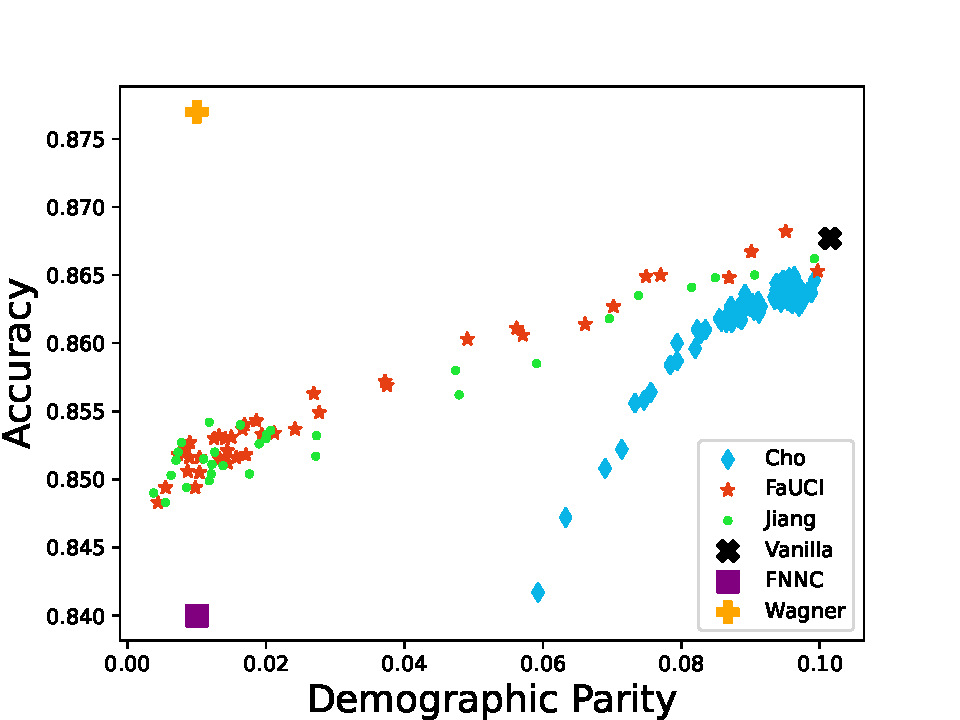
\includegraphics[width=\columnwidth]{figures/fauci/accuracy/demographic_parity_sex}
        \caption{Sensitive attribute: sex}
        \label{fig:dp-sex}
    \end{subfigure}
    %
    \begin{subfigure}[]{\onethirdsize}
        \centering
        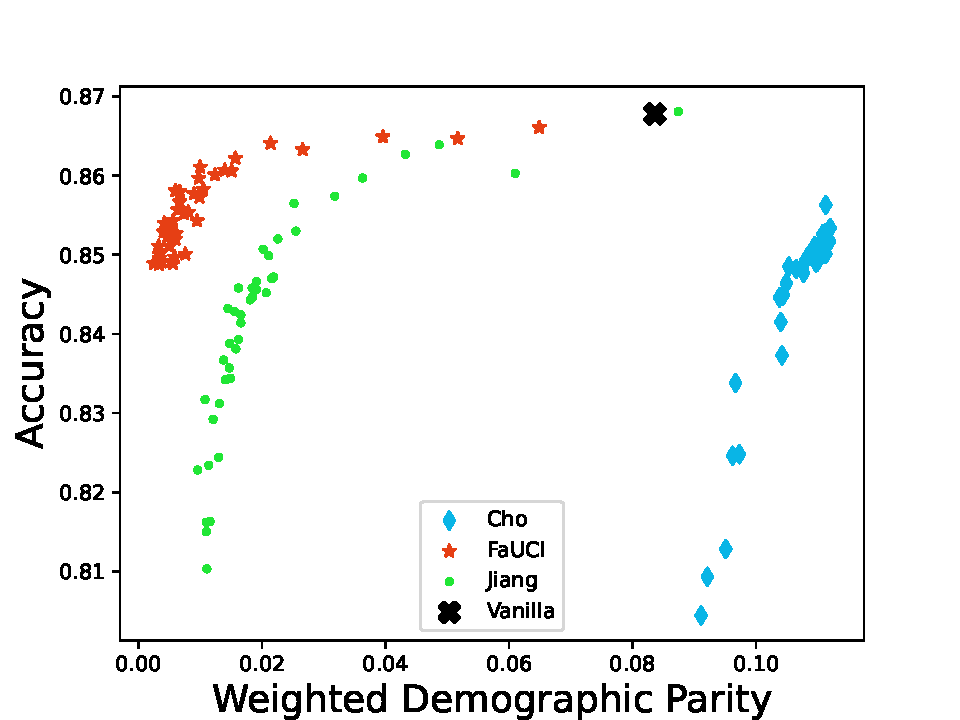
\includegraphics[width=\columnwidth]{figures/fauci/accuracy/demographic_parity_ethnicity}
        \caption{Sensitive attribute: ethnicity}
        \label{fig:dp-ethnicity}
    \end{subfigure}
    %
    \begin{subfigure}[]{\onethirdsize}
        \centering
        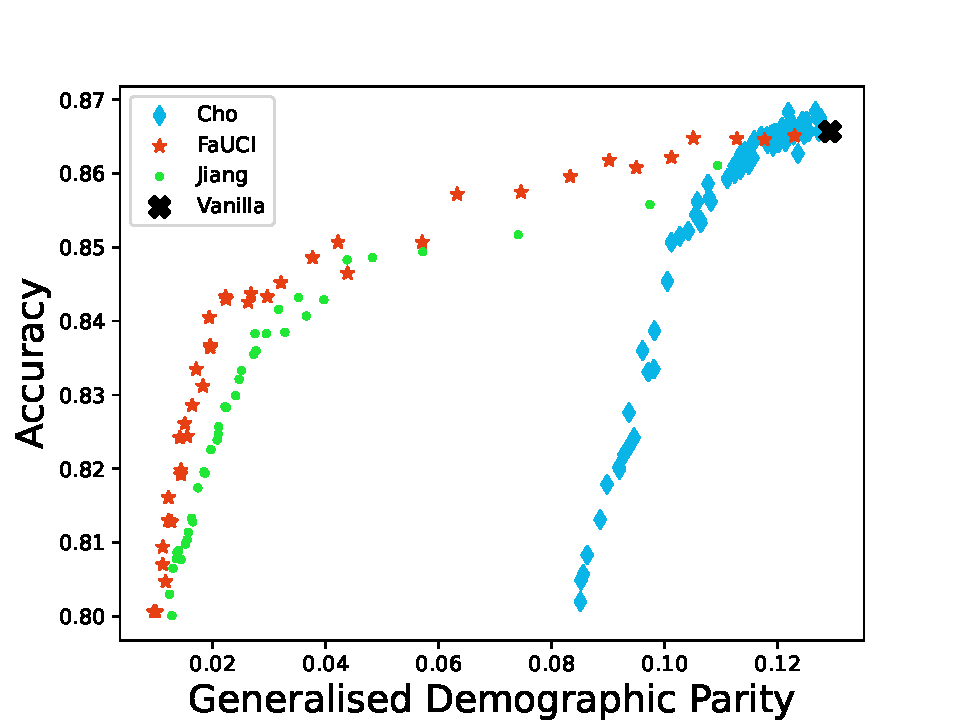
\includegraphics[width=\columnwidth]{figures/fauci/accuracy/demographic_parity_age}
        \caption{Sensitive attribute: age}
        \label{fig:dp-age}
    \end{subfigure}
    \label{fig:dp}
% \end{figure*}
% %
% \begin{figure*}[ht!]
%     \centering
%     \caption{%
%         Experiments applying DI constraints across different sensitive attributes. Legend as in \Cref{fig:dp}.
%         %
% %        Each dot is the average of 5 runs (5-folds cross-validation).
% %        %
% %        Red stars represent \fauci{}, the black cross the vanilla neural network (i.e., the NN without fairness constraints) and when possible, FNNC is represented as a purple square and Wagner's method as an orange cross.
%     }

    \begin{subfigure}[]{\onethirdsize}
        \centering
        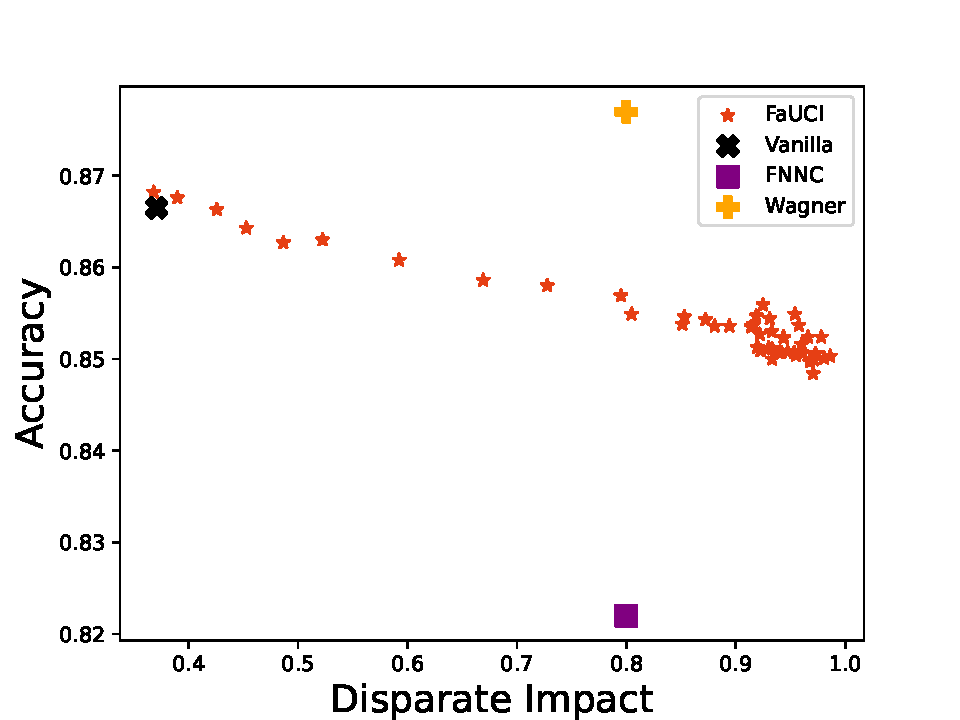
\includegraphics[width=\columnwidth]{figures/fauci/accuracy/disparate_impact_sex}
        \caption{Sensitive attribute: sex}
        \label{fig:di-sex}
    \end{subfigure}
    %
    \begin{subfigure}[]{\onethirdsize}
        \centering
        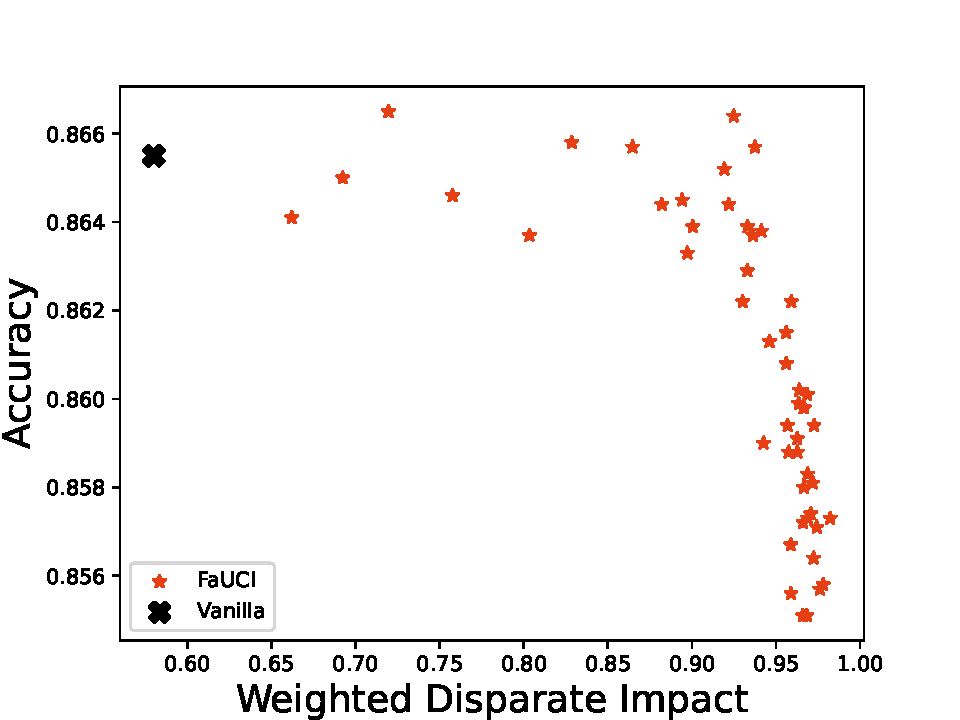
\includegraphics[width=\columnwidth]{figures/fauci/accuracy/disparate_impact_ethnicity}
        \caption{Sensitive attribute: ethnicity}
        \label{fig:di-ethnicity}
    \end{subfigure}
    %
    \begin{subfigure}[]{\onethirdsize}
        \centering
        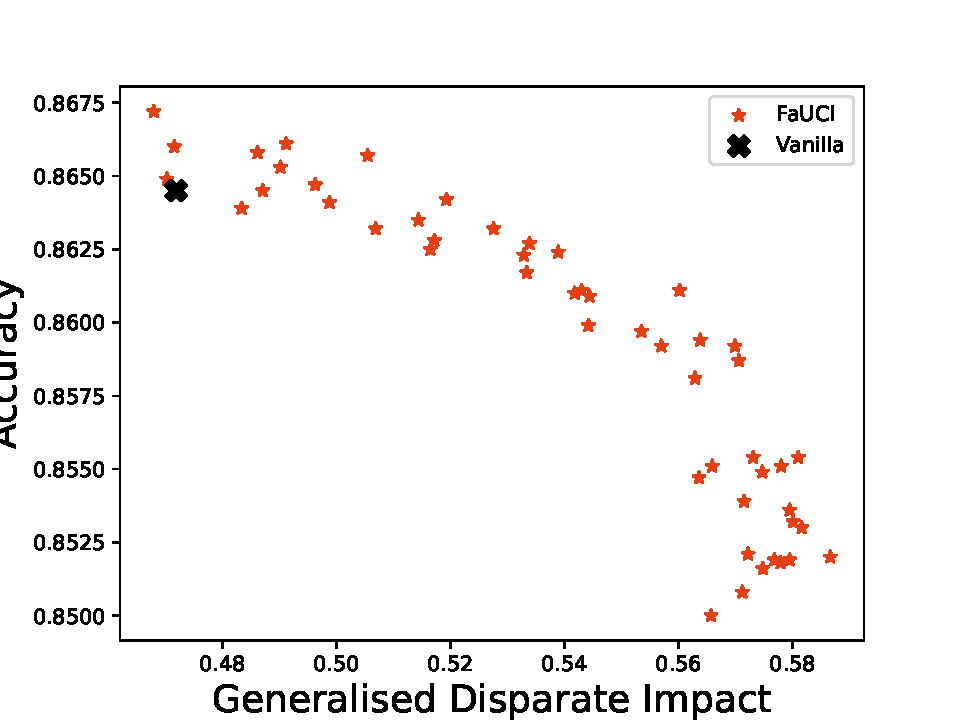
\includegraphics[width=\columnwidth]{figures/fauci/accuracy/disparate_impact_age}
        \caption{Sensitive attribute: age}
        \label{fig:di-age}
    \end{subfigure}
    \label{fig:di}
% \end{figure*}
% %
% \begin{figure*}[ht!]
%     \caption{%
%     	Experiments applying EO constraints across different sensitive attributes. Legend as in \Cref{fig:dp}.
%         %fairness methods results with different sensitive attributes.
%         %
% %        Each dot is the average of 5 runs (5-folds cross-validation).
% %        %
% %        Red stars represent our method, blue diamonds Cho's method, the black cross the vanilla neural network (i.e., the NN without fairness constraints) and when possible, FNNC is represented as a purple square.
%     }

    \begin{subfigure}[]{\onethirdsize}
        \centering
        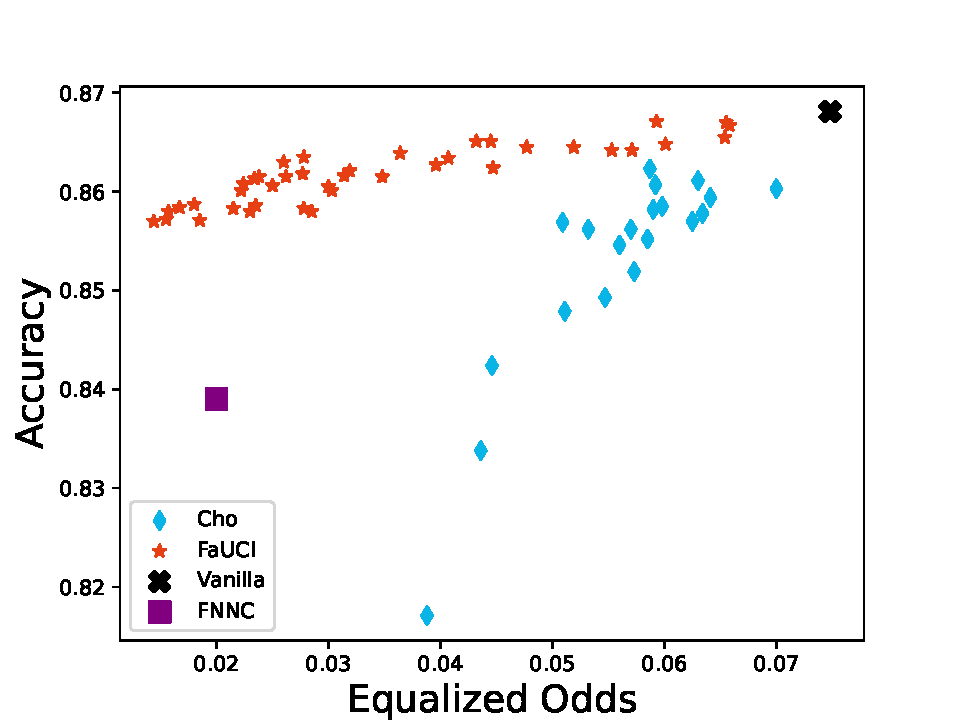
\includegraphics[width=\columnwidth]{figures/fauci/accuracy/equalized_odds_sex}
        \caption{Sensitive attribute: sex}
        \label{fig:eo-sex}
    \end{subfigure}
    %
    \begin{subfigure}[]{\onethirdsize}
        \centering
        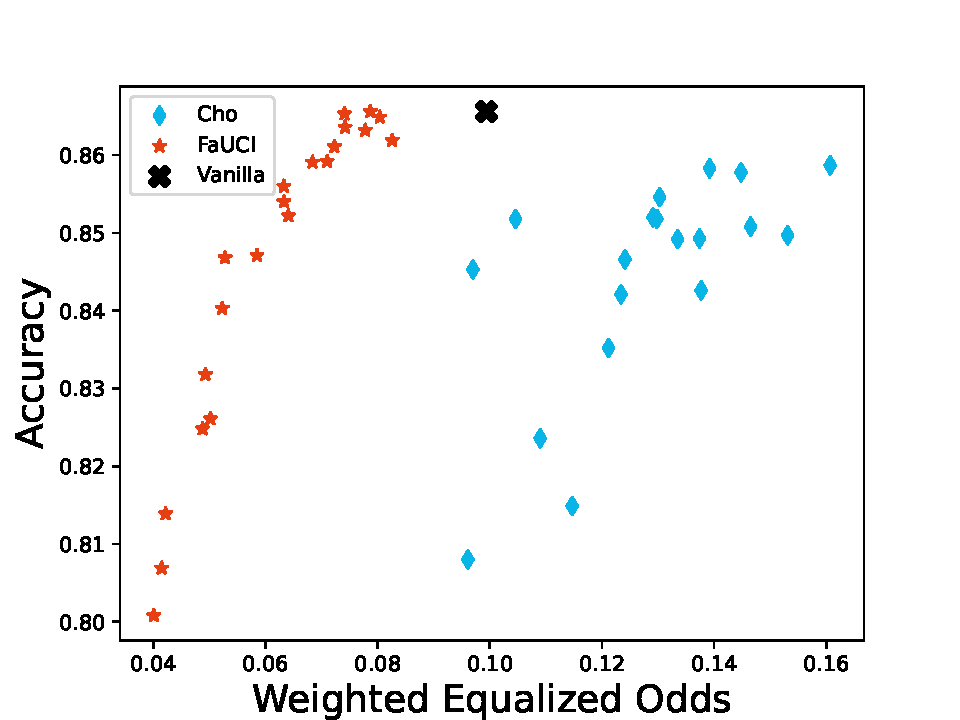
\includegraphics[width=\columnwidth]{figures/fauci/accuracy/equalized_odds_ethnicity}
        \caption{Sensitive attribute: ethnicity}
        \label{fig:eo-ethnicity}
    \end{subfigure}
    %
    \begin{subfigure}[]{\onethirdsize}
        \centering
        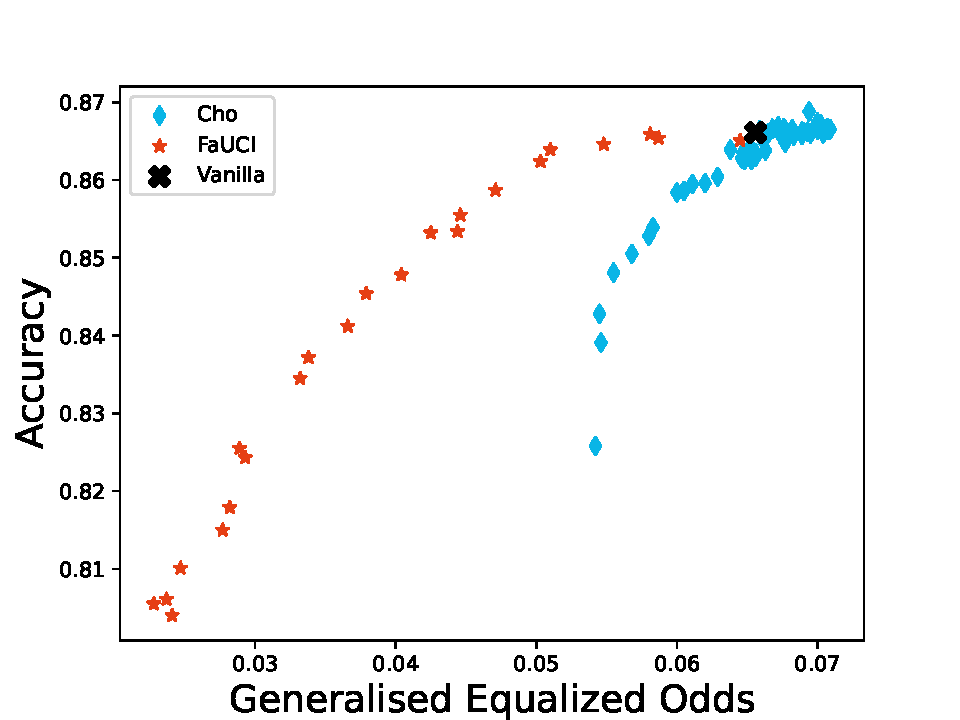
\includegraphics[width=\columnwidth]{figures/fauci/accuracy/equalized_odds_age}
        \caption{Sensitive attribute: age}
        \label{fig:eo-age}
    \end{subfigure}
    \label{fig:eo}
\end{figure}
%
\note{Update and improve the figures}
%
\paragraph{Demographic Parity Results}
%
\Cref{fig:dp} illustrates the trade-off between accuracy and \gls{DP} for \gls{FaUCI}, \gls{KDE}, \gls{GDP}, \gls{FNNC}, and \gls{NSIF} methods.
%
For \emph{sex} as a binary sensitive attribute, \gls{FaUCI} achieves an accuracy of \(85.27\%\) with \(\text{DP} \leq 0.01\), outperforming \gls{KDE} and matching \gls{GDP}'s performance.
%
\gls{FNNC} and \gls{NSIF} results are represented by single points, with accuracies of \(84\%\) and \(87.7\%\), respectively.
%
For \emph{ethnicity}, a categorical sensitive attribute, \gls{FaUCI} outperforms all methods, particularly when \(\text{DP} \leq 0.04\).
%
For \emph{age}, a continuous sensitive attribute, \gls{FaUCI} and \gls{GDP} perform similarly, but \gls{FaUCI} generally achieves better results.
%
Overall, \gls{FaUCI} demonstrates superior performance across all sensitive attributes.

%
\paragraph{Disparate Impact Results}
%
\Cref{fig:di} shows the trade-off between accuracy and \gls{DI}.
%
For \emph{sex}, \gls{FaUCI} achieves \(\text{DI} \geq 0.8\) with an accuracy of \(85.6\%\), surpassing \gls{FNNC} (\(82.2\%\)) and matching \gls{NSIF} (\(87.7\%\)).
%
For \emph{ethnicity}, \gls{FaUCI} maintains the accuracy of the uneducated model (\(86.8\%\)) while achieving \(\text{DI} \geq 0.8\).
%
For \emph{age}, \gls{FaUCI} improves \(\text{DI}\) to \(0.58\) with an accuracy of \(85.5\%\), though it does not reach the desired threshold of \(0.8\).
%
These results highlight \gls{FaUCI}'s ability to enhance \gls{DI} while preserving high accuracy.

%
\paragraph{Equalized Odds Results}
%
\Cref{fig:eo} presents the trade-off between accuracy and \gls{EO}.
%
For \emph{sex}, \gls{FaUCI} achieves \(\text{EO} \leq 0.02\) with an accuracy of \(\geq 85.9\%\), outperforming \gls{KDE} and \gls{FNNC} (\(83.9\%\)).
%
For \emph{ethnicity}, \gls{FaUCI} maintains high accuracy while reducing \gls{EO}, whereas Cho's accuracy drops significantly.
%
For \emph{age}, \gls{FaUCI} outperforms \gls{KDE} in both accuracy and \gls{EO}.
%
Overall, \gls{FaUCI} demonstrates consistent improvements in \gls{EO} while preserving a favorable accuracy-fairness trade-off.

\printbibliography[title=References,heading=bibintoc]
\end{refsection}

%----------------------------------------------------------------------------------------
%------------------------------------- PART III -----------------------------------------
%----------------------------------------------------------------------------------------

\part{Engineering of intelligent systems}\label{part:engineering-of-intelligent-systems}

\begin{refsection}
%! Author = matteomagnini
%! Date = 05/03/25

%----------------------------------------------------------------------------------------
\chapter{NeSy AI for real world applications}
\label{ch:nesy-ai-for-real-world-applications}

\begin{flushright}
\begin{minipage}{0.5\textwidth}
    How to apply \gls{SKI} and \gls{SKE} methods to design real-world \gls{AI} systems?

    How can \glspl{LLM} be exploited in the context of \gls{SKI} and \gls{SKE}?

    -- \textbf{\Cref{itm:rq0,itm:rq3,itm:rq4}}
\end{minipage}
\end{flushright}

\mtcaddchapter
\minitoc
%----------------------------------------------------------------------------------------


%
In this chapter we present a selection of contributions about \gls{NeSy} application in real-world scenarios.
%
These works involve the use of both \gls{SKE} and \gls{SKI} methods, as well as traditional \gls{ML} models and the recent \glspl{LLM}.


\section{\Gls{SKE} for explainable nutritional recommenders}\label{sec:ske-for-explainable-nutritional-recommenders}
%
``Symbolic knowledge extraction for explainable nutritional recommenders''~\cite{DBLP:journals/cmpb/MagniniCCAO23}, published on the Journal of Computer Methods and Programs in Biomedicine, presents a novel nutritional recommender system that leverages \gls{SKE}.


\subsection{Nutritional recommender systems}\label{subsec:nutritional-recommender-systems}

Eating habits significantly impact the well-being of individuals across all age groups, highlighting the importance of developing nutritional \glspl{RS}~\cite{EspinHN2016,Cioara2018,Shandilya2022}.
%
These systems address diverse user needs, including diet programs, chronic disease management, treatment for critically ill patients, allergies, lifestyle choices (e.g., sporty, vegetarian, organic, halal), and physical activity levels~\cite{Saiz2021,Hezarjaribi2019,AgapitoSCCLGPFC2018,FraserT1990,Tran2018}.
%
User preferences are represented either by expert knowledge, such as daily nutritional intake limits based on physical activity levels, or by user feedback, such as reviews on recipes~\cite{10.1145/3418211}.
%
Recommendation items, such as food, recipes, and meals, are represented in terms of their attributes, including cuisine, category, cooking style, preparation time, and nutritional levels.
%
The complexity of nutritional \glspl{RS} arises from the combination of multiple ingredients to form recipes and the diverse attributes influencing user preferences.

Classical approaches to nutritional recommendation rely on content based and collaborative filtering methods, which derive user profiles from past activities, such as ratings, clicks, reviews, and browsing history~\cite{Min2020}.
%
Recent advancements leverage \gls{ML} techniques, including question answering over knowledge bases, recipe retrieval from visual records of ingredients, and learning recipe representations from multi-modal data~\cite{Forbes2011,Bianchini2017,Freyne2010,Chen2021,Tian2022}.
%
Despite the availability of recipes online, many are suboptimal in terms of health~\cite{Trattner2017a}.
%
Recent studies aim to promote healthy eating by incorporating healthiness indicators into recommendations or enhancing the visual appeal of food~\cite{Saiz2021,10.1145/3418211}.
%
Providing explanations for recommendations improves user trust and acceptance, as transparent systems are preferred over black-box models~\cite{Anjomshoae2019}.
%
Explainable approaches, such as explanation ontologies and multi-agent architectures, have been proposed to enhance both personalisation and explainability in nutritional \glspl{RS}~\cite{DBLP:conf/icde/PadhiarSCGM21,Yera2022,expectation-extraamas2021}.

\subsection{Methodology}\label{subsec:methodology}
%
\begin{figure}
  \centering
  \includegraphics[width=\textwidth]{figures/ske-recommender-workflow}
  \caption[Data-flow perspective of a nutritional recommender system]{%
    Data-flow perspective of a nutritional \gls{RS}.
    %
    The user interacts -- via some smart/wearable device -- with a sub-symbolic AI predictor, continuously trained to predict whether the user likes a given recipe or not.
    %
    A knowledge base is then extracted from the predictor, representing the user's preferences in a human-interpretable logic form.
    %
    Dietary prescriptions -- provided by human experts -- are transformed into the same logic form.
    %
    Conversely, databases providing information about recipies -- there including ingredients and their nutrients -- are assumed to be remotely available via the Internet.
    %
    Finally, the recommending agent exploits a logic engine, combining all such information into recommendations which are simultaneously correct (w.r.t.\ experts prescriptions), acceptable (w.r.t.\ users' preferences), and explainable.
  }
  \label{fig:ske-recommender-workflow}
\end{figure}

We propose a general architecture for nutritional \glspl{RS}, designed to provide personalised dietary recommendations aligned with specific user goals.
%
\Cref{fig:ske-recommender-workflow} illustrates the main components and data flow within the system.
%
The proposed architecture personalises dietary recommendations by identifying recipes that lie at the intersection of user preferences and expert prescriptions.
%
This process relies on three distinct sources of information:
\begin{inlinelist}
    \item the user,
    \item the nutrition expert, and
    \item the recipe database.
\end{inlinelist}
%
Users provide their preferences, which are learned adaptively by a sub-symbolic \gls{ML} predictor.
%
Nutrition experts translate dietary goals into structured prescriptions, which define patterns of recipes suitable for achieving these goals.
%
The recipe database stores information about recipes, their ingredients, and corresponding nutrients, enabling the agent to propose admissible options.
%
Recommendations are generated by combining these sources using a logic-based approach, ensuring alignment with both user preferences and expert prescriptions.
%
In the following sections, we detail how preferences, prescriptions, and recipes are represented and manipulated within the system.
%
We also describe the algorithmic process for producing recommendations and discuss its underlying assumptions.


\paragraph{Recipes}\label{par:recipes}
%
Our architecture identifies three key data types: recipes, ingredients, and nutrients.
%
Recipes are composed of ingredients, which in turn contain various nutrients.
%
Each data type is named, meaning recipes, ingredients, and nutrients are uniquely identified by their names.
%
The architecture does not track the preparation process of meals but focuses on the nominal composition of ingredients and their quantities.
%
By analyzing the composition of ingredients in terms of nutrients, the system computes the overall nutritional values of recipes.
%
The recipes' database is responsible for storing information about recipes, ingredients, and nutrients.
%
It supports several types of queries, such as:
%
\begin{itemize}
  \item Selecting recipes based on their ingredients or nutrients.
  %
  \item Filtering recipes by specific quantities of ingredients or nutrients.
  %
  \item Retrieving the ingredients or nutrients associated with a recipe.
  %
  \item Clustering recipes with similar nutritional profiles.
\end{itemize}
%
These queries are essential for the recommender agent's functionality.


\paragraph{Users' Preferences}\label{par:users-preferences}
%
User preferences are represented sub-symbolically using a \gls{ML} predictor.
%
This predictor learns user tastes adaptively from data, which includes information about recipes the user likes or dislikes.
%
Preferences are modeled as a function:
%
\begin{equation}
  \label{eq:users-preferences}
  \text{appreciation}: R \to \mathbb{R}
\end{equation}
%
where \( R \) is the set of admissible recipes, and the output is an appreciation score.
%
Positive values indicate liking, negative values indicate dislike, and zero represents neutrality.
%
The appreciation score encapsulates user opinions, including factors such as taste, allergies, and ethical beliefs.
%
Data is collected during user interactions, often via smart or wearable devices, and used to train the \gls{ML} predictor.
%
The learning process is continual, ensuring the system adapts to evolving user preferences.
%
The sub-symbolic approach enables generalization of user data while leveraging information from the recipes' database.


\paragraph{Dietary Prescriptions}\label{par:dietary-prescriptions}
%
Dietary prescriptions are structured representations of what a user should eat and when, to achieve specific goals.
%
They are typically created by nutrition experts based on the user's physiological characteristics and expert knowledge.
%
Prescriptions consist of two components:
%
\begin{itemize}
  \item The \emph{what} component specifies ingredients or nutrients and their quantities for each meal.
  %
  \item The \emph{when} component indicates the time of consumption (e.g., breakfast, lunch, dinner).
\end{itemize}
%
The goal reflects the expected long-term effect on the user's health, though it may not be explicitly stated.
%
Prescriptions are often provided in quasi-natural language or tabular formats.
%
In tabular form, each cell corresponds to a specific time and meal, listing the recommended nutrients or ingredients.
%
Users may construct recipes based on these suggestions unless a nutritional \gls{RS} is available.
%
For simplicity, we focus on a single prescription for a given time \( t \), expressed as logic formulas.
%
These formulas define the properties a meal should have to align with dietary goals.
%
Details on the use of logic formulas for dietary prescriptions are provided in the next subsection.


\paragraph{The role of logic formulas}\label{par:the-role-of-logic-formulas}

The proposed architecture utilizes Horn clauses to represent both user preferences and expert prescriptions.
%
Horn logic provides a clear and computationally tractable framework for expressing dietary prescriptions.
%
These formulas can be manually written by humans or algorithmically generated, enabling their use in \glspl{RS} for dietary recommendations.

%
Expert prescriptions at time \( t \) are defined as a set of Horn clauses describing the \texttt{should\_eat/1} predicate.
%
This predicate specifies the recipes that the user should consume, based on admissible or forbidden ingredients and nutrients.
%
Two auxiliary predicates, \texttt{has/2} and \texttt{has\_no/2}, are used to assert the presence or absence of specific ingredients or nutrients.
%
Groups of ingredients or nutrients can also be defined using unary predicates, such as \texttt{vegetable/1}.

%
For example, a dietary prescription for Monday lunch can be expressed as:
%
\begin{align*}
  \begin{array}{rcl}
    \texttt{should\_eat}(R) &\leftarrow& \texttt{has}(R, \texttt{rice}) \land \texttt{has}(R, \texttt{chicken}) \\
                            &\land& \texttt{has\_no}(R, \texttt{salt}) \\
                            &\land& \texttt{has}(R, X) \land \texttt{vegetable}(X)
  \end{array}
\end{align*}
%
indicating that the user should consume recipes containing rice, chicken, and any vegetable, but excluding salt.

%
To ensure self-containment, additional rules must define the semantics of predicates such as \texttt{has/2}, \texttt{has\_no/2}, and \texttt{vegetable/1}.
%
For brevity, these definitions are omitted here.

%
Alternative encodings, such as including a predicate \texttt{quantity(X, Q)} to specify the quantity \( Q \) of ingredient \( X \), are possible but do not alter the core contribution.
%
Thus, simpler syntactic choices are preferred.

%
User preferences can also be represented as Horn clauses, defining the \texttt{likes/1} predicate.
%
These clauses may use the same auxiliary predicates (\texttt{has/2}, \texttt{has\_no/2}) and custom predicates for grouping ingredients or nutrients.

%
Consider the following example:
%
\begin{align*}
  \begin{array}{rcl}
    \texttt{likes}(R) &\leftarrow& \texttt{has}(R, \texttt{rice}) \land \texttt{has}(R, \texttt{chicken}) \\
                      &\land& \texttt{has\_no}(R, \texttt{broccoli}) \land \texttt{has}(R, \texttt{peas}) \\
    \texttt{vegetable}(\texttt{peas}) &\leftarrow \\
    \texttt{vegetable}(\texttt{broccoli}) &\leftarrow \\
    \texttt{has}(\texttt{paella}, \texttt{rice}) &\leftarrow \\
    \texttt{has}(\texttt{paella}, \texttt{chicken}) &\leftarrow \\
    \texttt{has}(\texttt{paella}, \texttt{peas}) &\leftarrow \\
    \texttt{has}(\texttt{paella}, \texttt{seafood}) &\leftarrow
  \end{array}
\end{align*}
%
This example states that the user likes recipes containing rice, chicken, and peas (e.g., paella), but dislikes broccoli.
%
It also defines peas and broccoli as vegetables and specifies the composition of paella.

%
When both prescriptions and preferences are expressed as Horn clauses, their intersection can be computed using logic resolution.
%
This involves proving the query:
%
\begin{equation}
    \label{eq:intersection-prescriptions-preferences}
    \texttt{likes}(R) \land \texttt{should\_eat}(R)
\end{equation}
%
against the merged clause set of prescriptions and preferences.
%
The logic solver identifies recipes \( R \) that satisfy both conditions or determines that no such recipes exist.

%
For instance, testing the query above against the merged clauses from the examples provided yields \( R = \texttt{paella} \).
%
This result is denoted as:
%
\begin{equation}
  \label{eq:intersection-prescriptions-preferences-final}
  (3) \cup (4) \models \texttt{likes}(\texttt{paella}) \land \texttt{should\_eat}(\texttt{paella})
\end{equation}


\paragraph{The role of \gls{SKE}}\label{par:the-role-of-ske}
%
Our proposed architecture requires both user preferences and expert prescriptions to be expressed as sets of Horn clauses.
%
This representation enables the use of logic resolution to construct recommendations.
%
Expert prescriptions are typically provided in formats, such as timetables of suggested recipes, that can be directly expressed or automatically converted into Horn clauses~\cite{DBLP:journals/jcss/Makowsky87}.
%
This assumption aligns with current practices in dietary planning.
%
In contrast, user preferences are modeled using sub-symbolic predictors, such as trained \glspl{NN}, which adaptively learn preferences from data.
%
While sub-symbolic representations are effective for capturing dynamic user preferences, they are incompatible with direct logic resolution.
%
To bridge this gap, the architecture incorporates a \gls{SKE} step.
%
This step extracts symbolic knowledge in the form of Horn clauses from the sub-symbolic predictor trained to model user preferences.
%
The choice of \gls{SKE} algorithm is left to the implementer, allowing flexibility to select the most suitable method for their application.
%
However, the extraction process must produce Horn clauses to ensure compatibility with the logic-based recommendation framework.
%
This approach combines the adaptability of sub-symbolic models with the interpretability and computational efficiency of symbolic reasoning.


\subsection{Validation}\label{subsec:validation-ske-nutrition}
%
To validate the proposed architecture, we conducted a series of experiments to assess its effectiveness in nutritional \glspl{RS}.
%
The source code and instructions for reproducing these experiments are public available\footnote{\url{https://github.com/pikalab-unibo/mccao-cmpb-experiments-2022}}
%
The experiments involved four main steps:
%
\begin{enumerate}
  \item Generating synthetic datasets to simulate a single user's food preferences.
  %
  \item Training a \gls{ML} predictor, specifically a neural network, to predict whether a recipe would be liked by the user.
  %
  \item Applying a \gls{SKE} algorithm to extract symbolic knowledge that represents the decision-making behavior of the predictor.
  %
  \item Evaluating the system's ability to recommend recipes that align with both user preferences and expert nutritional prescriptions.
\end{enumerate}
%
Details regarding data selection, synthesis, and experimental procedures are provided in the following subsections.

\paragraph{Datasets}\label{par:datasets-ske-nutrition}
%
We utilized a public dataset of recipes\footnote{available at \url{https://cosylab.iiitd.edu.in/culinarydb}} and generated 12 synthetic datasets to represent the preferences of imaginary users.
%
The recipe dataset consists of four files:
%
\begin{itemize}
  \item \textbf{Recipe Details:} Contains recipe IDs, titles, sources, and cuisines.
  %
  \item \textbf{Ingredients:} Lists basic ingredients with aliases, synonyms, entity IDs, and categories.
  %
  \item \textbf{Compound Ingredients:} Includes compound ingredients with their constituent components and categories.
  %
  \item \textbf{Recipe-Ingredients Aliases:} Maps recipes to their ingredients using aliases and entity IDs.
\end{itemize}
%
The dataset includes 929 unique basic ingredients and 103 compound ingredients, categorized into 21 groups (e.g., additive, bakery, beverage).
%
Recipes with at least one ingredient total 45,749, while recipes without ingredients are excluded.

Synthetic datasets were created in two steps.
%
First, unconditional preferences for individual ingredients were generated based on predefined user profiles.
%
Each profile specifies ranges of values for ingredients or categories (e.g., vegetables, meat), which are used to compute likelihoods via uniform distribution.
%
Second, recipe likability labels (like/dislike) were generated based on the likelihood values of the recipe's ingredients.
%
The synthesis process ensures no real personal data is used, avoiding ethical or privacy concerns.


\subsubsection{Learning User Preferences via Sub-Symbolic Predictors}\label{subsubsec:learning-user-preferences}
%
User preferences were modeled using fully-connected neural networks.
%
Each network consists of one input layer, two hidden layers, and one output layer, with 1032, 16, 8, and 1 neurons, respectively.
%
The activation functions for the input and hidden layers are \gls{ReLU}, while the output layer uses a sigmoid function.
%
The input to the network is a tensor representing the presence of 1032 ingredients in a recipe, and the output is a scalar indicating the likelihood of user appreciation.

A separate neural network was trained for each of the 12 synthetic users.
%
Training was performed on half of the dataset (22,874 records), while the remaining half was used for testing.
%
The training process lasted 20 epochs with a batch size of 32.
%
The average accuracy achieved on the test set was 85.6\%, with precision computed as the ratio of true positives to total positive predictions.
%
Precision is critical for systems where identifying true positives (liked recipes) is more important than minimizing false positives.

\subsubsection{Extracting User Preferences via \Gls{SKE}}\label{subsubsec:extracting-user-preferences}
%
\begin{table}%[!h]
    \centering
    \caption{
        Datasets statistics for each users on test sets.
        %
        The second column shows the \emph{like} class ratio.
        %
        Third and fourth columns describe the accuracy and precision score of trained neural networks.
        %
        Fifth and sixth columns describe the accuracy and precision score of the extracted rules.
        %
        The last column shows the fidelity of the extracted rules w.r.t.\ the NN.
    }
    % \begin{adjustbox}{width=\linewidth,center}
        \begin{tabular}{l||r|r|r|r|r|r}
            \textbf{users} & \textbf{liked ratio} & \textbf{net acc.} & \textbf{net prec.} & \textbf{r. acc.} & \textbf{r. prec.} & \textbf{r. fid.}\\
            \hline\hline
            user 1 & 0.336 & 0.9233 & 0.8855 & 0.864 & 0.8228 & 0.873\\
            user 2 & 0.2842 & 0.9714 & 0.9564 & 0.794 & 0.7688 & 0.7972\\
            user 3 & 0.3941 & 0.8503 & 0.8221 & 0.7726 & 0.7136 & 0.7955\\
            user 4 & 0.4502 & 0.8364 & 0.8165 & 0.7562 & 0.7145 & 0.7813\\
            user 5 & 0.3022 & 0.9621 & 0.9478 & 0.8381 & 0.8301 & 0.842\\
            user 6 & 0.2719 & 0.9722 & 0.9514 & 0.7997 & 0.7109 & 0.8034\\
            user 7 & 0.3504 & 0.8916 & 0.8369 & 0.7782 & 0.7311 & 0.7901\\
            user 8 & 0.449 & 0.7782 & 0.7594 & 0.6868 & 0.674 & 0.7283\\
            user 9 & 0.393 & 0.8085 & 0.7783 & 0.7493 & 0.7524 & 0.803\\
            user 10 & 0.4734 & 0.7381 & 0.7582 & 0.6862 & 0.7452 & 0.7616\\
            user 11 & 0.4359 & 0.7708 & 0.7863 & 0.7098 & 0.7426 & 0.7804\\
            user 12 & 0.4353 & 0.7772 & 0.7979 & 0.7047 & 0.7467 & 0.7814\\
            \hline\hline
            average & 0.3813 & 0.8567 & 0.8414 & 0.7616 & 0.7461 & 0.7948\\
        \end{tabular}
    % \end{adjustbox}
\label{tab:net-rules-stats}
\end{table}
%
Symbolic knowledge was extracted from the trained \gls{ML} predictors using the CART algorithm~\cite{DBLP:books/wa/BreimanFOS84}.
%
This algorithm generates decision trees, which are converted into logic rules.
%
Each path from the root to a leaf in the decision tree corresponds to a rule, where nodes represent logical conditions (e.g., presence or absence of ingredients) and leaves denote the predicted class.

The maximum number of leaves was set to \( R = 50 \), and the maximum depth of the decision tree was limited to \( D = 10 \).
%
These constraints balance computational efficiency and interpretability, ensuring the rules are concise and comprehensible.
%
For example, extracted rules for a user might include:
%
\begin{align*}
  \text{likes}(R) &\leftarrow \text{has\_no}(R, \text{egg}) \land \text{has\_no}(R, \text{pepper}) \land \text{has}(R, \text{almond}) \\
  \neg \text{likes}(R) &\leftarrow \text{has}(R, \text{egg}) \land \text{has}(R, \text{parsley})
\end{align*}
%
These rules approximate the decision-making process of the neural network, enabling explainability.

We constrain the output rules for two main reasons.
%
First, limiting the growth of the decision tree (\gls{DT}) reduces computational complexity.
%
Given \(N\) binary features, such as ingredients, the maximum depth of the \gls{DT} is \(N + 1\), and the maximum number of leaves is \(2^N\).
%
For \(N = 1032\), this would be computationally infeasible.
%
Second, we aim to ensure the extracted rules remain interpretable.
%
Rules with excessively long right-hand sides or an overwhelming number of conditions are difficult for humans to read and understand.
%
This trade-off prioritizes interpretability over performance metrics, such as accuracy and precision, which is essential for explaining why a prescription may or may not be suitable for a user.

\Cref{tab:net-rules-stats} summarizes the accuracy of the extracted rules on the test sets.
%
It also reports the fidelity of the rules with respect to the sub-symbolic predictors.
%
Fidelity is computed similarly to accuracy but compares the predictions of the extracted rules against the class values predicted by the \gls{ML} predictor, rather than the ground truth.
%
In other words, fidelity measures how closely the extracted rules replicate the behavior of the neural networks.


\subsubsection{Proposed Recipes}\label{subsubsec:proposed-recipes}
%
\begin{table}%[!h]
    \centering
    \caption[Precision of proposed recipes per user and prescription]{%
        Precision values of the algorithm per user and prescription. Precision values denote actually liked recipes (i.e., true positive) over the all proposed recipes (i.e., true positive plus false positive) obtained by prescriptions and extracted rules.
    }
    % \begin{adjustbox}{width=\linewidth,center}
        \begin{tabular}{l||r|r|r|r|r|r||r}
            \textbf{users} & \textbf{p. 1} & \textbf{p. 2} & \textbf{p. 3} & \textbf{p. 4} & \textbf{p. 5} & \textbf{p. 6} & \textbf{average}\\
            \hline\hline
            user 1 & 0.831 & 0.8 & 0.8621 & 0.6667 & 0.6875 & 0.7857 & 0.7722\\
            user 2 & 0.6338 & 0.2979 & 0.8 & 0.7083 & 0.9268 & 0.7727 & 0.6899\\
            user 3 & 0.7625 & 0.4333 & 0.7297 & 0.75 & 0.6111 & 0.6604 & 0.6578\\
            user 4 & 0.75 & 0.6 & 0.8387 & 0.65 & 0.5435 & 0.7755 & 0.693\\
            user 5 & 0.8571 & 0.7667 & 0.95 & 0.7083 & 0.8182 & 0.8095 & 0.8183\\
            user 6 & 0.6 & 0.5116 & 0.8636 & 0.8261 & 0.55 & 0.619 & 0.6617\\
            user 7 & 0.7625 & 0.4667 & 0.1852 & 0.8276 & 0.7391 & 0.7826 & 0.6273\\
            user 8 & 0.85 & 0.75 & 0.9048 & 0.5758 & 0.6667 & 0.7872 & 0.7558\\
            user 9 & 0.6316 & 0.9 & 0.8929 & 0.8085 & 0.8936 & 0.6809 & 0.8012\\
            user 10 & 0.875 & 0.66 & 0.7692 & 0.7879 & 0.717 & 0.7692 & 0.763\\
            user 11 & 0.8625 & 0.84 & 0.963 & 0.7391 & 0.64 & 0.8113 & 0.8093\\
            user 12 & 0.7875 & 0.8333 & 0.9024 & 0.8108 & 0.7037 & 0.8776 & 0.8192\\
            % \hline
            % \hline
            % average & 0.767 & 0.655 & 0.8051 & 0.7383 & 0.7081 & 0.761 & 0.7391\\
        \end{tabular}
        % \end{adjustbox}
    \label{tab:proposed-recipes-stats}
\end{table}


%
\begin{table}%[!h]
    \centering
    \caption{
        Precision values of the algorithm per user and prescription. Note that precision values denote actually liked recipes (i.e., true positive) over the all proposed recipes (i.e., true positive plus false positive) obtained by prescriptions and NN.
    }
    % \begin{adjustbox}{width=\linewidth,center}
        \begin{tabular}{l||r|r|r|r|r|r||r}
           \textbf{users} & \textbf{p. 1} & \textbf{p. 2} & \textbf{p. 3} & \textbf{p. 4} & \textbf{p. 5} & \textbf{p. 6} & \textbf{average}\\
            \hline\hline
            user 1 & 0.8267 & 0.8333 & 1.0 & 0.9474 & 0.8696 & 0.8913 & 0.8947\\
            user 2 & 0.95 & 0.9474 & 0.931 & 1.0 & 0.95 & 0.94 & 0.9531\\
            user 3 & 0.7875 & 0.7797 & 0.7273 & 0.8478 & 0.88 & 0.8163 & 0.8064\\
            user 4 & 0.775 & 0.7833 & 0.871 & 0.8158 & 0.7442 & 0.7447 & 0.789\\
            user 5 & 0.9265 & 0.9333 & 0.9565 & 0.9474 & 0.9524 & 0.9375 & 0.9423\\
            user 6 & 0.9375 & 0.9833 & 1.0 & 0.9615 & 0.9592 & 0.9583 & 0.9666\\
            user 7 & 0.8 & 0.8667 & 0.9 & 0.8571 & 0.8723 & 0.8913 & 0.8646\\
            user 8 & 0.8625 & 0.7833 & 0.8837 & 0.7 & 0.8077 & 0.8065 & 0.8073\\
            user 9 & 0.7875 & 0.7833 & 0.9118 & 0.8095 & 0.6786 & 0.6842 & 0.7758\\
            user 10 & 0.8125 & 0.5667 & 0.8049 & 0.7632 & 0.7959 & 0.84 & 0.7639\\
            user 11 & 0.8875 & 0.7667 & 0.7674 & 0.8723 & 0.7917 & 0.7931 & 0.8131\\
            user 12 & 0.825 & 0.8667 & 0.8049 & 0.68 & 0.8246 & 0.8364 & 0.8063\\
            % \hline
            % \hline
            % average & 0.8482 & 0.8245 & 0.8799 & 0.8502 & 0.8439 & 0.845 & 0.8486\\
        \end{tabular}
        % \end{adjustbox}
    \label{tab:proposed-recipes-stats-nn}
\end{table}


%
The experiments aim to evaluate how user preferences and expert prescriptions are combined to recommend recipes.
%
We rely on sets of logic rules to express domain-expert prescriptions, ensuring consistency with the formalism used for user preferences.
%
In total, six prescriptions are defined, corresponding to three days with two meals per day.
%
For each meal, multiple rules (ranging from two to four) are specified, one for each dish.

\begin{prescriptions}
  \item First day, lunch: ``Rice with vegetables.'' Ingredients include 80 grams of raw rice, 35 grams of raw lentils, 120 grams of raw chicken, 120 grams of mixed vegetables, garlic, herbs, 2 teaspoons of olive oil, and 1 orange.
  %
  \begin{align*}
    \begin{array}{rcl}
    \text{should\_eat}(R) & \leftarrow & \text{has}(R, \text{chicken}) \land \text{has}(R, \text{rice}) \\
    \text{should\_eat}(R) & \leftarrow & \text{has}(R, \text{lentils}) \\
    \text{should\_eat}(R) & \leftarrow & \text{has}(R, \text{orange}) \\
    \text{should\_eat}(R) & \leftarrow & \text{has}(R, \text{garlic})\\
                          & \land & \text{has}(R, X) \land \text{has}(R, Y) \land \text{has}(R, Z)\\
                          & \land & \text{vegetable}(X) \land \text{herb}(Y) \land \text{essential\_oil}(Z)
    \end{array}
  \end{align*}
  %
  \item First day, dinner: ``Burger and grilled vegetables.'' Ingredients include 90 grams of beef, 80 grams of bread, 120 grams of vegetables, 1 teaspoon of oil, and 1 cup of strawberries.
  %
  \begin{align*}
    \begin{array}{rcl}
      \text{should\_eat}(R) &\leftarrow& \text{has}(R, \text{beef}) \land \text{has}(R, \text{bread}) \\
      \text{should\_eat}(R) &\leftarrow& \text{has}(R, \text{strawberry}) \\
      \text{should\_eat}(R) &\leftarrow& \text{has}(R, X) \land \text{has}(R, Y) \\
                            &\land& \text{vegetable}(X) \land \text{essential\_oil}(Y)
    \end{array}
  \end{align*}
  %
  \item Second day, lunch: ``Tuna salad.'' Ingredients include 120 grams of tuna, 120 grams of vegetables, 1 teaspoon of olive oil, 80 grams of bread, 35 grams of raw beans, and 1 cup of blueberries.
  %
  \begin{align*}
    \begin{array}{rcl}
      \text{should\_eat}(R) &\leftarrow& \text{has}(R, \text{bread}) \land \text{has}(R, \text{beans}) \\
      \text{should\_eat}(R) &\leftarrow& \text{has}(R, \text{tuna}) \\
                            &\land& \text{has}(R, X) \land \text{has}(R, Y) \\
                            &\land& \text{vegetable}(X) \land \text{herb}(X) \land \text{essential\_oil}(Y) \\
      \text{should\_eat}(R) &\leftarrow& \text{has}(R, \text{blueberry})
    \end{array}
  \end{align*}
  %
  \item Second day, dinner: ``Chicken with mustard and lemon juice.'' Ingredients include 90 grams of chicken, 120 grams of vegetables, 80 grams of raw pasta, 1 teaspoon of olive oil, mustard, lemon juice, and 1 cup of clementines.
  %
  \begin{align*}
    \begin{array}{rcl}
      \text{should\_eat}(R) &\leftarrow& \text{has}(R, \text{chicken}) \land \text{has}(R, \text{mustard}) \land \text{has}(R, \text{lemon\_juice}) \\
      \text{should\_eat}(R) &\leftarrow& \text{has}(R, \text{pasta}) \\
                            &\land& \text{has}(R, X) \land \text{essential\_oil}(X) \\
      \text{should\_eat}(R) &\leftarrow& \text{has}(R, X) \land \text{vegetable}(X) \\
      \text{should\_eat}(R) &\leftarrow& \text{has}(R, \text{citrus\_fruits})
    \end{array}
  \end{align*}
  %
  \item Third day, lunch: ``Salmon with potatoes.'' Ingredients include 120 grams of salmon, 240 grams of cooked potatoes, 120 grams of vegetables, 1 teaspoon of butter, and 1 pear.
  %
  \begin{align*}
    \begin{array}{rcl}
      \text{should\_eat}(R) &\leftarrow& \text{has}(R, \text{compound\_salmon}) \land \text{has}(R, \text{potato}) \\
      \text{should\_eat}(R) &\leftarrow& \text{has}(R, \text{pear}) \\
      \text{should\_eat}(R) &\leftarrow& \text{has}(R, \text{butter}) \\
                            &\land& \text{has}(R, X) \land \text{vegetable}(X)
    \end{array}
  \end{align*}
  %
  \item Third day, dinner: ``Turkey in papillote.'' Ingredients include 90 grams of turkey, 1 teaspoon of olive oil, 120 grams of vegetables, 35 grams of raw gram beans, 80 grams of raw wholegrain rice, and 1 orange.
  %
  \begin{align*}
    \begin{array}{rcl}
      \text{should\_eat}(R) & \leftarrow & \text{has}(R, \text{gram\_bean}, \\
      \text{should\_eat}(R) & \leftarrow & \text{has}(R, \text{rice}) \\
      \text{should\_eat}(R) & \leftarrow & \text{has}(R, \text{orange}) \\
      \text{should\_eat}(R) & \leftarrow & \text{has}(R, \text{turkey}) \\
                            & \land & \text{has}(R, X) \land \text{has}(R, Y) \\
                            & \land & \text{vegetable}(X) \land \text{essential\_oil}(Y)
    \end{array}
  \end{align*}
\end{prescriptions}
%
For each user and prescription, recipes are computed based on the logic rules.
%
Precision is calculated as the ratio of recipes liked by users to the total number of proposed recipes.
%
Corner cases, where no recipes are recommended due to conflicting preferences and prescriptions, are resolved by adjusting prescriptions to better align with user preferences.


\subsection{Results and Discussion}\label{subsec:results-and-discussion}
%
To ensure realistic experiments, we adopted criteria to generate synthetic datasets representing user preferences.
%
We avoided synthesizing users with trivial rules, such as always liking a specific ingredient, which would result in predictable recommendations.
%
To address this, we introduced noise into the dataset synthesis process, assigning preference values within distributions and stochastically labeling classes.
%
This approach discourages oversimplified logic rules and mimics real-life scenarios where diverse ingredient combinations influence user preferences in complex ways.
%
\Cref{tab:net-rules-stats} reports the accuracy of the neural networks trained to predict user preferences, alongside the accuracy and fidelity of the extracted logic rules.
%
The accuracy of individual networks ranges from \(0.74\) to \(0.97\), with a mean value of approximately \(0.86\).
%
This variability reflects differences in user profiles, as some preferences are inherently more predictable than others.
%
The accuracy of the extracted rules ranges from \(0.68\) to \(0.86\), with a mean value of \(0.76\).
%
The mean difference of \(0.095\) between network accuracy and rule accuracy is expected, given the constraints imposed on decision tree depth during the extraction process.
%
Similar observations apply to precision measures.
%
It is important to note that extracted rules approximate the decision-making process of the neural networks and cannot outperform the original models.

\Cref{tab:proposed-recipes-stats-nn} summarizes the precision obtained during the recommendation phase using prescriptions and extracted rules.
%
The mean precision value across all experiments is approximately \(0.74\), which is close to the average precision of the rules reported in \Cref{tab:net-rules-stats}.
%
Applying the Student's \(t\)-test to the precision values in \Cref{tab:net-rules-stats} (``r. prec.'' column) and \Cref{tab:proposed-recipes-stats} (``average'' column) yields a \(p\)-value of \(0.386\).
%
This indicates no statistical difference between the two distributions.
%
In other words, recommending recipes liked by users from the entire dataset is as effective as recommending recipes prescribed by human experts.

\Cref{tab:proposed-recipes-stats-nn} compares the precision obtained using prescriptions and sub-symbolic predictors.
%
Similar statistical analysis yields a \(p\)-value of \(0.403\), leading to the same conclusion: the recommendation process is equally effective for prescribed liked recipes and liked recipes predicted by neural networks.

In summary, experiments demonstrate that sub-symbolic predictors outperform symbolic predictors in terms of overall precision for personalized food recommendations.
%
However, the primary goal of the framework is not to achieve higher performance compared to sub-symbolic predictors or existing systems.
%
Instead, the focus is on enhancing explainability, enabling users and experts to understand why certain recipes are recommended or rejected.
%
Extracted rules provide insights that allow experts to adjust prescriptions to better align with user preferences.
%
Despite lower performance compared to neural networks, the rules remain acceptable in real-world scenarios.
%
For instance, consider the recipe ``Shakkara (Sweet) Pongal'' (recipe ID \(4,055\)), which is liked by User~1.
%
This recipe contains ingredients such as basmati rice, butter, camphor, cardamom, cashew nuts, lentils, milk, raisins, and sugar.
%
The recommendation is justified by the presence of milk and sugar, as indicated by the extracted rules for User~1.
%
Conversely, the recipe ``Lasagna Spinach Roll-Ups'' (recipe ID \(10,815\)) is disliked due to the presence of eggs and pepper.
%
The symbolic approach adds value by providing explainability, allowing motivations for recommendations to be derived systematically.



\section{A general-purpose protocol for multi-agent based explanations}\label{sec:a-general-purpose-protocol-for-multi-agent-based-explanations}
%
In section we present the work ``A General-Purpose Protocol for Multi-agent Based Explanations''~\cite{DBLP:conf/extraamas/CiattoMBAO23}, presented at the \gls{EXTRAAMAS} international workshop, 5th edition, 2023.
%
This contribution is quite different from the previous one, and in general from the other contributions in this thesis.
%
While the majority of the works presented in this thesis vertically focus on \gls{SKI} or \gls{SKE} methods, or on the design of systems that leverage such methods, this work is more horizontal, in the sense that it proposes a general-purpose protocol for multi-agent based explanations.
%
Nonetheless, this work still falls within the scope of this chapter because its contribution is relevant to the design of explainable \glspl{MAS} that can potentially leverage \gls{SKE} methods.


\subsection{Motivation}\label{subsec:introduction-general-purpose-protocol-for-multi-agent-based-explanations}
%
The current focus of \gls{XAI} research is on developing techniques to ``open up'' black-box models and provide insights into how an intelligent system reaches specific decisions or predictions~\cite{DBLP:journals/csur/GuidottiMRTGP19}.
%
These techniques include methods for visualizing the internal workings of the system, such as feature importance scores, attention maps, and decision trees.
%
The primary goal of these methods is to assist \gls{AI} experts in understanding the system's behavior, rather than addressing the needs of non-expert users who seek to understand \emph{why} the system behaves in a particular way.

However, the expectations of the \gls{XAI} community extend beyond merely interpreting black-box models.
%
Ideally, \gls{XAI} systems should autonomously provide explanations that go beyond describing how the system works~\cite{DBLP:conf/aiia/CiattoCOC19}.
%
These explanations should offer insights into \emph{why} the system behaves -- or fails to behave -- in a specific manner, potentially through autonomous interaction with the explainee.

To achieve this, recent research emphasizes the automation and interactivity of the explanation process~\cite{DBLP:conf/atal/CiattoSOC20}.
%
This involves designing \gls{AI} systems capable of generating explanations dynamically and tailoring them to the explainee's knowledge level and needs.
%
In this context, \glspl{MAS} emerge as a suitable paradigm for building intelligent explainable systems, as they inherently support interaction and autonomy.
%
Explanations can thus be modeled as multi-agent interactions, where the explainee and the explainer agent (either human or software) collaborate to achieve the shared goal of providing clear and effective explanations.

This work addresses the general problem of enabling interaction between explainee and explainer agents.
%
To this end, it proposes a general-purpose protocol for multi-agent-based recommendations and explanations.
%
The protocol defines the roles and responsibilities of the explainee and explainer agents, as well as the types of information exchanged to ensure clarity and effectiveness.
%
Notably, the protocol builds upon prior efforts to model explanations as multi-agent interactions~\cite{buzcu-prima-2022}.
%
Its key features include:
%
\begin{inlinelist}
    \item the separation of recommendations from explanations, and
    \item support for contrastive explanations.
\end{inlinelist}

As a secondary contribution, the paper introduces a \texttt{Spade}-based Python library, \texttt{PyXMas}, which implements the proposed protocol.
%
This library allows the integration of various explanation strategies and representations.
%
It serves as a foundation for developing intelligent explainable systems where recommendation and explanation behaviors are delegated to individual agents.
%
Overall, this contribution represents a significant step toward building \gls{XAI} systems capable of providing automatic and interactive explanations.


\subsection{Background}\label{subsec:background-general-purpose-protocol-for-multi-agent-based-explanations}
%
\paragraph{Interactive recommendation systems}
%
Interactive \glspl{RS} have gained significant attention due to their ability to dynamically provide personalised recommendations based on user feedback and interactions~\cite{knijnenburg-2010}.
%
The key aspect of interactivity lies in collecting user feedback during the recommendation session to refine subsequent recommendations.
%
For instance, some systems employ a one-shot recommendation approach, where questions learned offline from past interactions are posed to users before generating recommendations~\cite{christakopoulou-2016}.
%
The answers to these questions enable the system to personalise and improve future suggestions.

\Gls{XAI} has been increasingly integrated into \glspl{RS} to enhance transparency~\cite{buzcu-prima-2022,zhang-2020}.
%
This is achieved through iterative recommendation sessions, where the system not only provides recommendations but also explanations, leveraging the positive impact of transparency on user trust~\cite{odonovan-2008}.
%
For example, visual explanations, such as grouped bar charts, have been used to compare user preferences with recommendation attributes~\cite{millecamp-2019}.
%
Similarly, conversational explanations have been employed to mimic human salesmanship, persuading users to consider alternative options~\cite{shimazu-2002}.


\paragraph{Prior work on explanation protocols}
%
This work builds upon the protocol introduced in~\cite{buzcu-prima-2022}, which focuses on food recommendations and explanations.
%
In this protocol, users specify constraints, such as allergies, preferred or disliked ingredients, and desired cuisine types.
%
The system responds with a recipe suggestion and an explanation.
%
Users can accept, reject, or provide feedback on the recommendation or explanation, initiating a turn-based interaction until the session concludes.
%
This framework promotes transparency by combining recommendations and explanations, which can increase user acceptance.
%
However, unrequested explanations may impose cognitive load, highlighting the importance of parsimony~\cite{MuallaTKNCAGN22}.
%
Parsimonious explanations are defined as the simplest descriptions that adequately convey the situation.

To address this, the revised protocol proposed in this work allows users to request explanations dynamically.
%
It also supports ``zooming'' explanations, where additional details are provided only upon user request.
%
This approach enables users to control the level of detail, ensuring explanations are tailored to their needs.


\paragraph{\textsc{Spade}: multi-agent programming in python}
%
\textsc{Spade} is an open-source \gls{MAS} platform implemented in Python\footnote{\url{https://spade-mas.readthedocs.io}}.
%
It provides a modular and extensible library for developing intelligent agents capable of interacting with each other and their environment.
%
\textsc{Spade} systems are distributed, with agents operating on the same or different network nodes.
%
Agent activities are governed by concurrent behaviours, implemented as Python classes that developers can extend.

Unlike \textsc{Jade}~\cite{jadebook-2007}, which is Java-based, \textsc{Spade} leverages Python's ecosystem, facilitating integration with \gls{ML} and \gls{AI} frameworks.
%
Agent communication in \textsc{Spade} is mediated by the \gls{XMPP} protocol, ensuring robust, interoperable, and scalable interactions.
%
This design supports blended applications where agents interact with both humans and software agents.

\textsc{Spade} includes features such as communication protocols, message passing, and event handling.
%
It also supports the implementation of interaction protocols using finite-state machine behaviours.
%
These capabilities make \textsc{Spade} a powerful tool for developing intelligent agents, widely adopted in \gls{MAS} research and development.


\subsection{Explanation-based recommendation protocol}
\label{subsec:explanation-based-recommendation-protocol}
%
The term ``explanation'' originates from the Latin word \emph{explicare}, meaning ``to unfold.''
%
In this context, an explanation is understood as the process of clarifying the meaning of a concept.
%
This process is inherently interactive, involving an explainee and an explainer.
%
Explanations are thus considered a social protocol.

In human interactions, explanation protocols are typically informal and unstructured.
%
They involve an explainee seeking clarification from an explainer, who is assumed to possess greater knowledge.
%
Explainers adapt their strategies and level of detail to the explainee's needs and knowledge as the interaction progresses.
%
Explanations are generally provided upon request and may respond to prior information shared by either party.

Modern intelligent systems, such as \gls{XAI} systems, aim to support decision-making by providing recommendations.
%
In these systems, the user typically acts as the explainee, while the software system assumes the roles of both the recommender and the explainer.
%
By adopting a \gls{MAS} perspective, recommendation and explanation can be modeled as a single interaction protocol between two agents.
%
One agent, often the explainee, is a human user, while the other, the explainer, is a software agent.

The proposed protocol assumes that the user initiates the interaction by submitting a query.
%
Upon receiving the query, the agent generates a recommendation.
%
This recommendation is computed using available information, such as the user's profile, interaction history, and possibly aggregated data from other users.
%
The agent may utilize both symbolic reasoning and \gls{ML} predictors to generate the recommendation.

%
After receiving the recommendation, the user may either accept or reject it, or request an explanation.
%
The explanation phase may involve multiple rounds of interaction, where the user can ask for additional details or comparisons.
%
The agent provides the requested information, aiming to clarify the recommendation.
%
Ultimately, the user decides to accept or reject the recommendation based on the explanation provided.

Feedback from the user, including the acceptance or rejection of recommendations and the amount of explanatory information required, is used to improve future interactions.
%
In cases of rejection, the agent may also seek the reason for the rejection to refine its recommendation and explanation strategies.


Explanations in this protocol are always:
%
\begin{inlinelist}
    \item provided upon request,
    \item related to the recommendation, and
    \item tailored to the user.
\end{inlinelist}
%
They can be categorized into two types:
%
\begin{itemize}
    \item \textbf{Ordinary explanations:} These address the question, ``Why did you recommend this?''
    %
    \item \textbf{Contrastive explanations:} These address the question, ``Why did you not recommend that instead?''
\end{itemize}
%
The protocol supports both types of explanations, allowing the user to choose the type they prefer.
%
The content and structure of the exchanged messages depend on the type of explanation requested.


\subsection{Abstract Formulation of the Protocol}
\label{subsec:abstract-formulation-of-the-protocol}
%
\begin{figure}
    \centering
    \includegraphics[width=\linewidth]{figures/pyxmas/user-agent-protocol}
    \caption[Message communication diagram between an explainer agent and an explainee]{%
      Message communication diagram between an explainer agent (blue boxes) and an explainee (green boxes).
      %
      Each box represents a message.
      %
      Arrows indicate the possible replies to each message.
    }
    \label{fig:protocol-messages}
\end{figure}
%
\Cref{fig:protocol-messages} presents an abstract formulation of the proposed protocol, which is independent of the specific representation or computation of recommendations and explanations.
%
The focus is on the exchange of messages between the explainer and the explainee, the information these messages carry, and the sequence in which they are exchanged.
%
The protocol defines two roles:
%
\begin{itemize}
    \item The explainee, who initiates the interaction.
    %
    \item The explainer, who responds to the explainee's queries.
\end{itemize}
%
Five data types are identified as the potential payloads exchanged during the protocol:
%
\begin{itemize}
    \item \textbf{Queries} (\(Q\)): Requests for recommendations submitted by the explainee.
    %
    \item \textbf{Recommendations} (\(R, R'\)): Responses to queries, provided by the explainer.
    %
    \item \textbf{Explanations} (\(E, E'\)): Information provided by the explainer to clarify recommendations.
    %
    \item \textbf{Features} (\(F\)): User-specific aspects that justify the rejection of a recommendation, which the explainer should consider in future interactions.
    %
    \item \textbf{Motivations} (\(M\)): Reasons for rejecting a recommendation, which may influence the explainer's behavior.
\end{itemize}
%
Thirteen message types are defined, each represented as a named record of the form \texttt{Name(Payload)}, where \texttt{Payload} consists of instances of the aforementioned data types.
%
Optional fields in the payload are denoted with a question mark.
%
The message types are summarized as follows:
%
\begin{enumerate}
    \item \texttt{Query(\(Q\))}: Sent by the explainee to initiate the protocol, carrying a recommendation request.
    %
    \item \texttt{Recommendation(\(Q, R\))}: Sent by the explainer in response to a query, carrying the query and the computed recommendation.
    %
    \item \texttt{Why(\(Q, R\))}: Sent by the explainee to request an explanation for a recommendation.
    %
    \item \texttt{WhyNot(\(Q, R, R'\))}: Sent by the explainee to request a contrastive explanation, comparing the recommendation with an alternative.
    %
    \item \texttt{Accept(\(Q, R, E?\))}: Sent by the explainee to accept a recommendation, optionally including the explanation.
    %
    \item \texttt{Collision(\(Q, R, F, E?\))}: Sent by the explainee to notify the explainer of a conflict between the recommendation and a personal feature.
    %
    \item \texttt{Disapprove(\(Q, R, M, E?\))}: Sent by the explainee to reject a recommendation, providing a reason and optionally the explanation.
    %
    \item \texttt{Details(\(Q, R, E\))}: Sent by the explainer to provide additional details about a recommendation.
    %
    \item \texttt{Comparison(\(Q, R, R', E\))}: Sent by the explainer to provide a contrastive explanation when the alternative recommendation is also valid.
    %
    \item \texttt{Invalid(\(Q, R', E\))}: Sent by the explainer to indicate that the alternative recommendation is invalid, with an explanation.
    %
    \item \texttt{Unclear(\(Q, R, E\))}: Sent by the explainee to indicate that the provided explanation is unclear.
    %
    \item \texttt{Prefer(\(Q, R, R'\))}: Sent by the explainee to express a preference for an alternative recommendation.
    %
    \item \texttt{Override(\(Q, R, R'\))}: Sent by the explainee to enforce an alternative recommendation, even if deemed invalid by the explainer.
\end{enumerate}
%
This abstract formulation ensures flexibility, allowing implementers to tailor the protocol to specific application domains.

Notably, messages are designed by keeping the \gls{ReST} [9] architectural style into account.
%
Hence, each message type is designed to carry all the information necessary for any involved party to decide which action to take next.
%
This is the reason why all/most messages carry the original query $Q$ and the recommendation $R$ (or $R'$) which they are referring to.
%
The message communication diagram from \Cref{fig:protocol-messages} depicts not only the messages exchanged by the explainee and explainer, but also the admissbile request-response patterns which the protocol allows.
%
There, a more detailed view of the message flow is provided, which we briefly summarise in the following.


\subsubsection{Relevant scenarios and protocol analysis}\label{subsubsec:relevant-scenarios}
%
% !TeX spellcheck = en_GB
% !TeX root = ../phd-thesis.tex

\begin{figure}
    \centering{
        \begin{subfigure}[t]{0.4\linewidth}
            \centering
            \includegraphics[width=\linewidth]{figures/quick-accept}
            \caption{Quick accept: the user accepts the recommendation without asking for explanations.}
            \label{fig:quick-accept}
        \end{subfigure}
        \hfill%\vline\hfill
        \begin{subfigure}[t]{0.4\linewidth}
            \centering
            \includegraphics[width=\linewidth]{figures/quick-retry}
            \caption{Quick retry: the user rejects the recommendation without asking for explanations. Another recommendation is proposed, accordingly.}
            \label{fig:quick-retry}
        \end{subfigure}
    }

    \medskip

    \centering{
        \begin{subfigure}[t]{0.4\linewidth}
            \centering
            \includegraphics[width=\linewidth]{figures/explanation-loop}
            \caption{Ordinary explanation loop: the user asks `why' after a recommendation, and then agent answers with further details. The request for details may be repeated several times.}
            \label{fig:explanation-loop}
        \end{subfigure}
        \hfill%\vline\hfill
        \begin{subfigure}[t]{0.4\linewidth}
            \centering
            \includegraphics[width=\linewidth]{figures/contrastive-explanation-loop}
            \caption{Contrastive explanation loop: the user asks `why not' another recommendation. The agent may then explain why the other recommendation is acceptable or invalid. The user may either accept the original recommendation or prefer their own.}
            \label{fig:contrastive-explanation-loop}
        \end{subfigure}
    }
    \caption{Sequence diagrams describing most common scenarios of the protocol.}
    \label{fig:protocol-sequence-diagrams}
\end{figure}

%
The proposed protocol is versatile and accommodates various user needs and desires.
%
These include:
%
\begin{inlinelist}
    \item requesting a recommendation,
    \item seeking an explanation for the recommendation,
    \item asking for additional details about the explanation,
    \item simulating alternative recommendations, and
    \item providing feedback on recommendations or explanations.
\end{inlinelist}
%
\Cref{fig:protocol-sequence-diagrams} illustrates these scenarios, which are detailed below.

%
\paragraph{Quick Accept}
%
In this scenario, depicted in \Cref{fig:quick-accept}, the user accepts the recommendation without requiring an explanation.
%
For example, a user requests a restaurant recommendation, and the agent suggests a restaurant that the user finds satisfactory.

%
\paragraph{Quick Retry}
%
In \Cref{fig:quick-retry} the user rejects the recommendation without asking for an explanation.
%
The rejection may occur because the recommendation conflicts with the user's preferences or is unsuitable for the current context.
%
For instance, if the agent recommends a steakhouse to a vegetarian user, the user may signal a conflict with their preferences.
%
Alternatively, the user may simply disapprove of the recommendation without providing specific feedback.
%
In both cases, the agent generates a new recommendation.
%
The agent is expected to learn from conflicts but not from generic disapprovals.

%
\paragraph{Ordinary Explanation Loop}
%
In the case shown in \Cref{fig:explanation-loop}, the user requests an explanation for the recommendation.
%
If the explanation is unsatisfactory, the user may ask for further details, initiating an iterative process.
%
This loop continues until the user either accepts the recommendation or requests a new one.
%
The protocol supports ``zooming'' explanations, where the agent adjusts the granularity of the explanation.
%
For example, the agent may first provide local explanations, describing how the specific recommendation was generated.
%
Subsequently, it may offer global explanations, detailing the general logic behind its recommendations.
%
The agent can also switch between textual and visual explanations to enhance clarity.
%
Consider a user who requests a restaurant recommendation.
%
The agent suggests an Asian restaurant with a high rating and proximity to the user.
%
If the user asks for an explanation, the agent may state that the restaurant matches the user's taste for sushi and is within 1 km.
%
If further details are requested, the agent may explain its general recommendation strategy, such as prioritizing highly rated restaurants within a certain distance.

%
\paragraph{Contrastive Explanation Loop}
%
Lastly, in \Cref{fig:contrastive-explanation-loop}, the user requests a contrastive explanation, comparing the given recommendation \(R\) with an alternative \(R'\).
%
If \(R'\) is valid, the agent provides a comparison, highlighting why one recommendation is preferable.
%
If \(R'\) is invalid, the agent explains why it cannot be recommended.
%
The user may then accept the original recommendation, prefer the alternative, or override the agent's decision.
%
For example, if the agent recommends an Asian restaurant, but the user prefers a steakhouse, the agent may compare the two options.
%
If the steakhouse aligns with the user's dietary goals, the agent may note that the Asian restaurant is closer.
%
If the steakhouse violates dietary goals, the agent explains this conflict.
%
In either case, the user decides whether to accept the original recommendation or override it.
%
The agent learns from overrides to refine future recommendations.


\subsubsection{Which Sorts of Explanations and Recommendations?}
\label{subsubsec:which-sorts-of-explanations-and-recommendations}

The proposed explanation protocol is agnostic regarding the specific representation of explanations and recommendations.
%
It is the responsibility of the implementer to define how explanations and recommendations are represented and computed.
%
The protocol only specifies \emph{when} these elements should be computed.

\Glspl{RS} typically rely on one or more \gls{ML} predictors trained on user data.
%
Whether the training of these predictors is performed by the recommender agent or if the agent is equipped with pre-trained predictors at deployment is an implementation detail.
%
In either case, the recommender agent must have access to user profile information.
%
This information can be obtained during an initial configuration phase or inferred from user interactions, such as accepted or rejected recommendations.
%
To support dynamic learning, the agent should include a learning algorithm capable of updating the predictors when new user data becomes available.
%
From this perspective, the explainer agent acts as a proxy for the \gls{ML} predictor(s).

Explanations, however, are not necessarily derived from \gls{ML} predictors.
%
The \gls{XAI} literature offers a wide range of approaches for generating explanations, including visual, textual, and numerical methods~\cite{DBLP:journals/inffus/ArrietaRSBTBGGM20,DBLP:journals/csur/GuidottiMRTGP19,DBLP:journals/csur/CiattoSAMO24}.
%
The explainer agent must not only wrap the \gls{ML} predictor(s) but also encapsulate the logic for computing and representing explanations.

A critical challenge arises when recommendations and explanations use different representation formats, such as textual and visual.
%
In such cases, the explainer agent must bridge the gap by providing a unified representation of both the recommendation and its explanation.
%
To address this, designers may consider adopting computational logic as a unifying framework for recommendations and explanations.
%
In computational logic, both knowledge bases and queries are represented as logic formulas.
%
These formulas can be used to represent recommendation requests, solutions, and explanations.

For example, a recommendation query can be expressed as the logic goal:
%
\[
\texttt{should\_eat(Food, lunch)},
\]
%
where \texttt{Food} is a logic variable representing an unknown value.
%
Recommendations, such as \( R, R', R'' \), correspond to logic solutions, e.g., \(\texttt{Food} = \texttt{paella}\).
%
Explanations \( E, E', E'' \) can take various forms:
%
\begin{itemize}
    \item \textbf{Local explanations:} The path in the proof tree computed by the explainer agent to derive the recommendation.
    %
    \item \textbf{Global explanations:} The logic program used by the explainer agent to generate the recommendation.
    %
    \item \textbf{Contrastive explanations:} Metrics comparing multiple recommendations or identifying constraints that make certain recommendations invalid.
    %
    \item \textbf{Combinations:} Any combination of the above types.
\end{itemize}

User features, such as \( F, F', F'' \), may include raw facts describing the user, e.g., \texttt{age(31)}, \texttt{goal(lose\_weight)}, or \texttt{category(vegetarian)}.
%
Motivations for disapproval can include predefined facts, such as:
%
\begin{itemize}
    \item \texttt{dislike:} The user dislikes the recommendation, prompting the agent to learn from this feedback.
    %
    \item \texttt{not\_now:} The user does not want the recommendation at the moment, but may accept it in the future.
    %
    In this case, the agent should not memorize the rejection.
    %
\end{itemize}


\subsection{From Theory to Practice with \textsc{PyXMas}}
\label{subsec:from-theory-to-practice-with-pyxmas}
%
\begin{figure}
    \centering
    \includegraphics[width=\linewidth]{figures/pyxmas/architecture}
    \caption[Modular architecture of \textsc{PyXMas}]{%
        Modular architecture of \textsc{PyXMas}.
        %
        The library provides parametric behaviours that can be customized by implementing specific components.
        %
        If the explainee agent is human, a UX component may be required to facilitate interaction via a device.
    }
    \label{fig:architecture}
\end{figure}
%
This section describes how the proposed protocol can be implemented as agent-oriented software.
%
We introduce \textsc{PyXMas}\footnote{\url{https://github.com/pikalab-unibo/pyxmas}}, a Python library for explainable multi-agent systems (\glspl{MAS}).
%
The library is built on \textsc{Spade} and provides reusable implementations of the protocol described in \Cref{subsec:abstract-formulation-of-the-protocol}.
%
This allows researchers and developers to focus on designing recommender and explainer agents, as well as defining the representation of recommendations and explanations, without re-implementing the protocol.


\subsubsection{\textsc{PyXMas} Architecture}
\label{subsubsec:pyxmas-architecture}
%
\Cref{fig:architecture} illustrates the modular architecture of \textsc{PyXMas}.
%
The library defines two main behaviours:
%
\begin{inlinelist}
    \item the \emph{initiator}, responsible for sending recommendation queries and processing responses, and
    %
    \item the \emph{responder}, responsible for computing and returning recommendations and explanations.
\end{inlinelist}
%
The initiator behaviour is designed for the explainee agent, while the responder behaviour is intended for the explainer agent.
%
Both behaviours are parametric, allowing users to customize their functionality by implementing specific components.

\paragraph{Explainer Agent}
%
The explainer agent requires the following components:
%
\begin{itemize}
    \item \textbf{Recommendation Strategy:} Computes recommendations based on user queries, preferences, and goals (e.g., ``vegetarian'' or ``weight loss'').
    %
    The strategy can adapt over time by learning from user feedback.
    %
    \item \textbf{Explanation Strategy:} Generates explanations for recommendations, leveraging user profiles and domain knowledge (e.g., ``ingredient X is plant-based'').
    %
    \item \textbf{User Profiler:} Learns user preferences from feedback using heuristic or \gls{ML}-based methods.
    %
    This enables the agent to refine recommendations and explanations dynamically.
    %
    \item \textbf{Interaction Strategy:} Manages how recommendations and explanations are presented to the explainee.
    %
    For example, a humanoid robot may use gestures or facial expressions to enhance interaction.
\end{itemize}
%
The explainer agent stores two types of data:
%
\begin{inlinelist}
    \item user profile data, and
    %
    \item domain knowledge.
\end{inlinelist}
%
These are maintained in dedicated data stores and updated as needed.

\paragraph{Explainee Agent}
%
The explainee agent requires the following components:
%
\begin{itemize}
    \item \textbf{Query Provider:} Generates queries based on the explainee's goals.
    %
    \item \textbf{Recommendation Evaluator:} Assesses recommendations and decides whether to accept or reject them.
    %
    \item \textbf{Explanation Evaluator:} Evaluates explanations and influences the recommendation evaluator accordingly.
\end{itemize}
%
If the explainee is a human user, the agent acts as a proxy, mediating interactions via a \gls{UI} on a device (e.g., a smartphone).
%
In this case, a \textbf{\gls{UX}} component is required to manage the \gls{UI}, process user inputs, and present recommendations and explanations.


\subsubsection{PyXMas Design}\label{subsubsec:pyxmas-design}
%
\begin{figure}
    \centering
    \includegraphics[width=0.7\linewidth]{figures/pyxmas/types}
    \caption{
        Abstract classes for message payloads in \textsc{PyXMas}.
    }
    \label{fig:types}
\end{figure}
%
\textsc{PyXMas} is a Python library designed for developing explainable \glspl{MAS}.
%
It provides:
%
\begin{itemize}
    \item Abstract classes for the (de)serialization of message payloads exchanged between the explainer and explainee agents (see \Cref{fig:types}).
    %
    \item Abstract classes defining the initiator and responder behaviors.
\end{itemize}
%
These abstract classes allow developers to extend and customize their functionality by overriding specific methods.
%
This flexibility enables the creation of tailored explainable \glspl{MAS}.
%
\paragraph{Data Types for Message Payloads}
%
As illustrated in \Cref{fig:types}, \textsc{PyXMas} provides five abstract classes corresponding to the data types defined in \Cref{subsec:abstract-formulation-of-the-protocol}.
%
These classes enforce serialization, ensuring that data can be converted to and from strings.
%
This is essential for enabling communication between the explainer and explainee agents over the network.
%
Developers can define custom representations for queries, recommendations, explanations, and other data types by extending these abstract classes.
%
The only requirement is that the serialized data must be both machine- and human-readable.
%
\paragraph{Predefined Behaviors}
%
\begin{figure}
    \centering
    \begin{subfigure}[t]{\linewidth}
        \centering
        \includegraphics[width=\linewidth]{figures/pyxmas/user-state-diagram}
        \caption{
            Initiator-side state diagram.
        }
        \label{fig:user-state-diagram}
    \end{subfigure}
    %
    \begin{subfigure}[t]{\linewidth}
        \centering
        \includegraphics[width=\linewidth]{figures/pyxmas/agent-state-diagram}
        \caption{
            Responder-side state diagram.
        }
        \label{fig:agent-state-diagram}
    \end{subfigure}
    \caption{
        State diagrams describing the initiator and responder behaviors in \textsc{PyXMas}.
    }
    \label{fig:state-diagrams}
\end{figure}
%
\textsc{PyXMas} provides two abstract classes for the protocol roles:
%
\begin{itemize}
    \item The \emph{initiator}, which represents the explainee agent.
    %
    \item The \emph{responder}, which represents the explainer agent.
\end{itemize}
%
These behaviors are implemented as finite-state machines (FSMs) using \textsc{Spade}.
%
Each state corresponds to a specific action, such as waiting for a message or processing a response.
%
\Cref{fig:state-diagrams} illustrates the state diagrams for the initiator and responder behaviors.
%
On the initiator side, developers can override callbacks to control:
%
\begin{itemize}
    \item Query generation.
    %
    \item Evaluation of recommendations and decisions to accept or reject them.
    %
    \item Evaluation of explanations and their influence on recommendation acceptance.
\end{itemize}
%
On the responder side, developers can override callbacks to control:
%
\begin{itemize}
    \item Recommendation generation.
    %
    \item Explanation generation.
    %
    \item Handling of accepted or rejected recommendations.
\end{itemize}
%
This design ensures that \textsc{PyXMas} can be adapted to various application domains while maintaining a clear and modular structure.


\section[\Gls{NeSy} \Gls{AI} for disease diagnosis and monitoring]{\Gls{NeSy} \gls{AI} for supporting Chronic disease diagnosis and monitoring}
\label{sec:nesy-ai-for-supporting-chronic-disease-diagnosis-and-monitoring}
%
\subsection{Motivations and background}
\label{subsec:motivations-and-background}
%
Telemedicine platforms are increasingly used for personal assistance, enabling patients to share their symptoms, medical history, and diagnostic data, such as medical images, lab results, or vital signs.
%
These platforms often leverage \gls{AI} data-driven models~\cite{HunterNEJMra2212850,topol2022}.
%
While promising, accurate disease monitoring and diagnosis require more than identifying patterns in data.
%
The integration of \gls{AI} into clinical practice remains limited due to several challenges.
%
First, the performance of \gls{AI} models is often suboptimal, primarily due to insufficient dataset sizes for effectively training \gls{ML} algorithms~\cite{benjamens2020state}.
%
Second, even high-performing \gls{AI} models frequently operate as black boxes, making their outputs difficult to interpret.
%
This lack of transparency hinders adoption in clinical settings, where healthcare professionals require interpretable outputs to make informed decisions~\cite{ALI2023107555}.
%
Traditional clinical protocols, while validated and robust, also exhibit limitations.
%
They often fail to classify all clinical cases, leaving certain scenarios unresolved.
%
Additionally, these protocols do not leverage data analytics, which could uncover hidden patterns and provide valuable insights for decision-making.

Combining data-driven and knowledge-based models has been identified as a promising solution to enhance \gls{ML} performance and improve explainability~\cite{von2021informed}.
%
This work focuses on \gls{NeSy} \gls{AI}, specifically \gls{SKI}~\cite{DBLP:journals/csur/CiattoSAMO24}.
%
Among the various \gls{SKI} methods, we evaluate the \gls{LTN} approach~\cite{BadreddineGSS22}.
%
The potential of this approach is demonstrated using the \gls{PID} dataset for diabetes prediction~\cite{smith1988using}.
%
We compare its performance against classical \gls{ML} models, including \gls{KNN}, \gls{LR}, \gls{DT}, \gls{RF}, and an uneducated \gls{MLP}.
%
Performance is evaluated based on criteria such as classification accuracy and robustness.

Results indicate that classical \gls{ML} models struggle to achieve consistent performance.
%
In contrast, injecting domain knowledge into neural networks via the \gls{LTN} method significantly improves clinically relevant metrics, such as recall, balanced accuracy, F1 score, and Matthews Correlation Coefficient~\cite{MATTHEWS1975442}.
%
Moreover, \gls{LTN} enhances adherence to clinical knowledge, a critical requirement in the medical domain.
%
It also demonstrates high robustness against data manipulation, including noise injection, data dropping, and label flipping.

\subsection{Knowledge integration in medicine}
\label{subsec:knowledge-integration-in-medicine}

The integration of medical knowledge into \gls{ML} pipelines can occur at various stages~\cite{von2021informed,kierner2023taxonomy}.
%
\begin{itemize}
    \item \textbf{Data pre-processing:} Errors in datasets can be mitigated by removing anomalous samples based on clinical norms.
    %
    Virtual samples adhering to medical knowledge can be generated to address insufficient or missing data.
    %
    \item \textbf{Feature engineering:} Novel features can be derived using mathematical or logical models informed by medical knowledge.
    %
    Feature selection can also be guided by prior knowledge.
    %
    \item \textbf{Model learning:} Rules can be incorporated into the model's loss function or architecture.
    %
    \item \textbf{Output evaluation:} \gls{ML} outputs can be integrated with clinical guidelines to filter predictions or verify consistency with domain knowledge.
\end{itemize}
%
While these strategies are promising, they often do not reference the \gls{SKI} framework or its complementary \gls{SKE} paradigm~\cite{DBLP:journals/csur/CiattoSAMO24}.
%
These paradigms have proven effective in other domains and hold potential for healthcare applications.
%
Preliminary experiments~\cite{sirocchiRuleML2024} suggest that further evaluation of \gls{SKI} methods, such as \gls{LTN}, is warranted.


\subsection{Materials and methods}
\label{subsec:materials-and-methods}
%
In this study, we utilize the \gls{PID} dataset~\footnote{\url{https://www.kaggle.com/datasets/uciml/pima-indians-diabetes-database}}, a widely recognized benchmark in medical-related \gls{ML} research~\cite{karegowda2011application,DBLP:journals/nca/ChangBXS23}.
%
We focus on the \gls{LTN} approach~\cite{BadreddineGSS22}, a \gls{SKI} method that combines structuring and constraining injection strategies.
%
This section details the dataset, the \gls{LTN} methodology, and the metrics used to evaluate the impact of \gls{SKI} on predictive performance and \gls{QoS} aspects.

%
\subsubsection{Dataset and knowledge}
\label{subsubsec:dataset-and-knowledge}
%
The \gls{PID} dataset consists of 768 medical profiles of women aged 21 and above who underwent an oral glucose tolerance test.
%
The dataset includes features such as glucose and insulin concentrations, blood pressure (BP), skin thickness (ST), body mass index (BMI), diabetes pedigree function, number of pregnancies, and age.
%
The target variable is binary, indicating whether diabetes was diagnosed within five years.

%
Missing values are present in several attributes, including insulin (48.70\%), ST (29.56\%), BP (4.55\%), BMI (1.43\%), and glucose (0.65\%).
%
These missing values were imputed using the median value of the respective attribute.
%
The dataset is imbalanced, with 65.1\% of instances labeled as negative and 34.9\% as positive.

%
Public health guidelines on type-2 diabetes risks indicate that individuals with a high BMI (\(\geq 30\)) and high blood glucose levels (\(\geq 126\)) are at severe risk for diabetes.
%
Conversely, individuals with a normal BMI (\(\leq 25\)) and low blood glucose levels (\(\leq 100\)) are less likely to develop diabetes.
%
These guidelines are encoded into logic formulas as follows:
%
\begin{align}
    \forall x.\, (\text{glucose}(x) \geq 125 \land \text{bmi}(x) \geq 30 \rightarrow \text{Diabetic}(x)), \label{eq:diabetes_rule1} \\
    \forall x.\, (\text{glucose}(x) \leq 100 \land \text{bmi}(x) \leq 25 \rightarrow \neg \text{Diabetic}(x)). \label{eq:diabetes_rule2}
\end{align}

%
\subsubsection{Logic Tensor Network for \gls{SKI}}
\label{subsubsec:ltn-for-ski}
%
The \gls{LTN} framework~\cite{BadreddineGSS22} extends \gls{FOL} with fuzzy semantics, where formulas are interpreted as continuous truth values in the interval \([0, 1]\).
%
This allows the definition of logic rules that are not strictly true or false but partially true, with predicates computed by neural networks.

%
In this study, we use \gls{LTN} to inject the knowledge encoded in Equations~\eqref{eq:diabetes_rule1} and~\eqref{eq:diabetes_rule2}.
%
The predicate \(\text{Diabetic}(x)\) is modeled as a neural predicate backed by a feed-forward \gls{NN} with three hidden layers.
%
The NN outputs a real number in \([0, 1]\), representing the truth value of \(\text{Diabetic}(x)\) for an input \(x \in \mathbb{R}^8\).

%
The training process maximizes the truth value of the logic formulas while considering the available data.
%
This is achieved by minimizing a loss function that penalizes violations of the injected knowledge.
%
The predicates \(\text{glucose}(x)\) and \(\text{bmi}(x)\) are grounded to the actual values in the dataset, while the following dummy formulas are added to supervise the training:
%
\begin{align}
    \forall x.\, (\text{outcome}(x) = \text{diabetes} \rightarrow \text{Diabetic}(x)), \\
    \forall x.\, (\text{outcome}(x) = \text{healthy} \rightarrow \neg \text{Diabetic}(x)).
\end{align}

%
\subsubsection{Evaluation Metrics}
\label{subsubsec:evaluation-metrics}
%
To assess the impact of \gls{SKI}, we evaluate both predictive performance and \gls{QoS} metrics.

%
\paragraph{Performance Metrics}
%
Predictive performance is evaluated using standard metrics for binary classification, including accuracy, precision, recall, F1-score, balanced accuracy (BA), and the \gls{MCC}.

%
\paragraph{Logic Adherence}
%
Inspired by fidelity metrics in the \gls{SKE} framework~\cite{DBLP:journals/csur/CiattoSAMO24}, we propose a metric to assess adherence to clinical rules.
%
For each rule, we create a test set of instances satisfying the rule, assign labels based on the rule, and compute the model's accuracy on this subset.

%
\paragraph{Quality of Service}
%
\gls{QoS} metrics evaluate non-functional aspects such as robustness and complexity.
%
This study focuses on robustness to data degradation, which occurs when input data is noisy, incomplete, or biased.
%
Robustness is quantified using a reproducible procedure where training data is perturbed, and the model's performance is evaluated on the perturbed data~\cite{DBLP:journals/aamas/AgiolloRMCO23}.
%
The robustness score \(\rho_{N, D}(D)\) of a predictor \(N\) trained on \(D\) is defined in \Cref{eq:robustness-score}.
%
The robustness gain \(R_{N, D}(I)\) of an injection mechanism \(I\) is computed as shown in \Cref{eq:robustness-gain}.
%
A value \(R_{N, D}(I) > 1\) indicates improved robustness, while \(R_{N, D}(I) < 1\) indicates reduced robustness.


\subsubsection{Experimental Design}
\label{subsubsec:experimental-design}
%
The experiments are designed to evaluate the impact of the \gls{LTN} approach on the performance of \gls{ML} models in a clinical context.
%
The implementation of \gls{LTN} used in this study is publicly available\footnote{\url{https://github.com/pikalab-unibo/experiments-ltn-2024}}, along with the code for replicating the experiments.
%
The evaluation focuses on three main aspects:
%
\begin{enumerate}
    \item The predictive performance of \gls{ML} models, with particular attention to recall and F1-score, given the medical domain's sensitivity to false negatives.
    %
    \item The adherence of \gls{ML} models to established medical protocols, assessing whether the educated model aligns more closely with the injected knowledge compared to the uneducated one.
    %
    \item The robustness of \gls{ML} models to data degradation, analyzing whether the performance of the educated model degrades less than that of the uneducated model under perturbed data.
\end{enumerate}
%
To ensure a fair comparison, a grid search is performed to optimize the hyperparameters of all models.
%
The best hyperparameters for the baseline models are as follows:
%
\begin{itemize}
    \item \gls{KNN}: \(k = 7\), L1 distance.
    %
    \item \gls{DT}: Entropy as the split criterion, maximum depth of 10.
    %
    \item \gls{RF}: 50 trees, maximum depth of 20, entropy as the criterion, and a minimum of 5 samples per leaf.
    %
    \item \gls{LR}: Regularization parameter of 10, maximum iterations of 1,000, and \texttt{liblinear} as the solver.
\end{itemize}
%
The uneducated \gls{MLP} and the educated \gls{LTN} models share the same feedforward \gls{NN} architecture:
%
\begin{itemize}
    \item An input layer with 8 neurons, one for each feature in the dataset, using the \gls{LeakyReLU}~\cite{maas2013rectifier} activation function and batch normalization.
    %
    \item Three hidden layers with 256, 128, and 64 neurons, respectively, each using \gls{LeakyReLU} and batch normalization.
    %
    \item An output layer with a single neuron and a sigmoid activation function.
\end{itemize}
%
The training of the \gls{LTN} model consists of two phases.
%
First, the uneducated model is trained for 50 epochs using the Adam optimizer with a learning rate of \(10^{-4}\), weight decay of \(10^{-4}\), a batch size of 32, and a binary cross-entropy loss function.
%
An early stopping criterion is applied, with a patience of 5 epochs.
%
Second, the knowledge is injected, and the model is fine-tuned for 200 epochs using the same early stopping criterion but with a reduced learning rate of \(10^{-6}\).
%
All models are evaluated using multiple runs of a 50--50 train-test split, with performance metrics averaged over 50 runs.
%
Statistical significance is assessed using the Wilcoxon signed-rank test with a significance level of 0.05.
%
To evaluate robustness, the experiments include multiple runs with different types and magnitudes of data perturbations.
%
The perturbations include noise addition, sample drop, and label flipping, following the methodology in~\cite{DBLP:journals/aamas/AgiolloRMCO23}.
%
The noise magnitude \(\mu\) ranges from 0.1 to 1.0 in steps of 0.1, while the percentages of sample drop and label flipping vary from 0 to 0.9 in steps of 0.1.


\subsection{Results and Discussion}
\label{subsec:results-discussion}
%
We now present and discuss the results obtained for predictive performance metrics, logical adherence, and robustness.

%
\subsubsection{Performance Metrics}
\label{subsubsec:performance-metrics}
%
\begin{table*}[]
    \centering
    \begin{adjustbox}{max width=\textwidth}
        \begin{tabular}{|l|c|c|c|c|c|c|}
            \hline
            \textbf{Model} & \textbf{Accuracy} & \textbf{Precision} & \textbf{Recall} & \textbf{F1 Score} & \textbf{Balanced Accuracy} & \textbf{MCC} \\
            \hline
            \gls{KNN}  & 0.738 $\pm$  0.02 & 0.636 $\pm$  0.03 & 0.583 $\pm$  0.05 & 0.607 $\pm$  0.03 & 0.702 $\pm$  0.02 & 0.413 $\pm$  0.05 \\
            \hline
            \gls{DT}   & 0.697 $\pm$  0.02 & 0.565 $\pm$  0.03 & 0.580 $\pm$  0.05 & 0.571 $\pm$  0.03 & 0.670 $\pm$  0.02 & 0.339 $\pm$  0.05 \\
            \hline
            \gls{RF}   & 0.758 $\pm$  0.02 & 0.677 $\pm$  0.03 & 0.592 $\pm$  0.05 & 0.630 $\pm$  0.03 & 0.720 $\pm$  0.02 & 0.456 $\pm$  0.04 \\
            \hline
            \gls{LR}   & \textbf{0.763 $\pm$  0.02 }& \textbf{0.702 $\pm$  0.04} & 0.560 $\pm$  0.04 & 0.622 $\pm$  0.03 & 0.716 $\pm$  0.02 & 0.460 $\pm$  0.04 \\
            \hline
            \gls{MLP}  & 0.754 $\pm$  0.02 & 0.644 $\pm$  0.03 & 0.665 $\pm$  0.05 & 0.653 $\pm$  0.03 & 0.733 $\pm$  0.02 & 0.464 $\pm$  0.04 \\
            \hline
            \gls{LTN}  & 0.747 $\pm$  0.02 & 0.620 $\pm$  0.03 & \textbf{0.725 $\pm$  0.05} & \textbf{0.666 $\pm$  0.02} & \textbf{0.742 $\pm$  0.02} & \textbf{0.471 $\pm$  0.03} \\
            \hline
        \end{tabular}
    \end{adjustbox}
%    \vspace{0.5em}
    \caption[Performance metrics for \gls{ML} models on the \gls{PID} Dataset]{
      Performance metrics (mean $\pm$ std) for \gls{ML} models.
      %
      The best scores are highlighted in bold.
      %
      According to the Wilcoxon signed-rank test with p-value=0.05, the \gls{LTN} model outperforms all other models in terms of Recall, F1 Score, and Balanced Accuracy.
    }
    \label{tab:ski-diabetes-performance-metrics}
%    \vspace{-3em}
\end{table*}
%
The performance metrics are summarized in \Cref{tab:ski-diabetes-performance-metrics}.
%
While \gls{LR} achieves the highest accuracy, this metric is less reliable for imbalanced datasets.
%
In this study, the minority class, representing diabetic instances, is the primary focus.
%
The \gls{LTN} model achieves the highest scores in balanced accuracy, F1-score, and \gls{MCC}.
%
These metrics are more suitable for evaluating clinical models as they account for class imbalance.
%
The \gls{LTN} also achieves the highest recall value of \(0.725\), which is critical in clinical settings.
%
Recall measures the proportion of diabetic patients correctly identified, minimizing false negatives.
%
False negatives can lead to missed diagnoses and untreated conditions, which are particularly problematic in healthcare.
%
In contrast, \gls{KNN} and \gls{DT} achieve recall values of \(0.583\) and \(0.580\), respectively, indicating their limited ability to detect positive cases.
%
\gls{LR} achieves a recall of \(0.560\), while \gls{RF} slightly improves with a recall of \(0.592\).
%
Although the \gls{MLP} shows some improvement with a recall of \(0.66\), the injection of domain knowledge via the \gls{LTN} yields a significant performance boost.
%
Precision, while highest for \gls{LR}, is less emphasized in clinical contexts, as false positives typically lead to follow-up testing with minimal consequences.
%
These results highlight the limitations of classical \gls{ML} models in achieving sufficient recall for clinical deployment.
%
The superior recall of the \gls{LTN} can be attributed to its incorporation of logic formulas, which effectively utilize background knowledge.
%
By grounding predictions in logical structures, the \gls{LTN} identifies patterns that simpler models may overlook.

%
\subsubsection{Logical Adherence}
\label{subsubsec:logical-adherence}
%
\begin{table}
  \centering
  \begin{adjustbox}{max width=0.8\textwidth}
    \begin{tabular}{|l|c|c|}
      \hline
      \textbf{Model} & \textbf{Rule 1} & \textbf{Rule 2} \\
      \hline
      \gls{KNN}  & 70.8 $\pm$  4.8   & 100.0 $\pm$  0.0 \\
      \hline
      \gls{DT}   & 66.5 $\pm$  6.3   & 97.0 $\pm$  4.8 \\
      \hline
      \gls{RF}   & 76.6 $\pm$  5.1   & 100.0 $\pm$  0.0 \\
      \hline
      \gls{LR}   & 75.0 $\pm$  4.2   & 100.0 $\pm$  0.0 \\
      \hline
      \gls{MLP}  & 82.0 $\pm$  5.8   & 100.0 $\pm$  0.0 \\
      \hline
      \gls{LTN}  & \textbf{87.4 $\pm$  5.2 }  & 100.0 $\pm$  0.0 \\
      \hline
    \end{tabular}
  \end{adjustbox}
%  \vspace{0.5em}
  \caption{
      Logic adherence results for Rule 1 and Rule 2 (mean $\pm$ std) across various models.
  }
  \label{tab:logic-adherence}
%  \vspace{-2em}
\end{table}
%
In clinical applications, models must not only make accurate predictions but also align with established medical protocols.
%
Adherence to clinical guidelines enhances trust and reliability, increasing the likelihood of adoption in practice.
%
The logical adherence results are presented in \Cref{tab:logic-adherence}.
%
All models, except for \gls{DT}, fully comply with the second rule, which classifies healthy patients.
%
However, the primary focus is on adherence to the first rule, which identifies diabetic patients.
%
The \gls{MLP} achieves \(82\%\) adherence to the first rule, outperforming classical \gls{ML} models such as \gls{RF}, which achieves \(76\%\).
%
The \gls{LTN} further improves adherence, achieving \(87\%\).
%
These results confirm that injecting domain knowledge through the \gls{LTN} modifies the model's structure, aligning it more closely with medical knowledge and clinical protocols.

%
\subsubsection{Robustness Analysis}
\label{subsubsec:robustness-analysis}
%
\begin{figure}
    \centering
    \includegraphics[width=\linewidth]{figures/ski-diabetes-robustness}
    \caption[Robustness analysis under noise injection, label flipping, and data dropping]{
        %
        Robustness analysis under noise injection, label flipping, and data dropping.
        %
        The \gls{LTN} demonstrates superior robustness across all metrics compared to other models.
    }
    \label{fig:robustness-analysis}
\end{figure}
%
Robustness refers to the model's ability to maintain performance under data perturbations, such as noise, missing data, or label flipping.
%
This evaluation is critical in clinical settings, where data collection is often noisy or incomplete.
%
The robustness results are illustrated in \Cref{fig:robustness-analysis}.
\note{TODO: generate again the figure because it is not vectorial and it has an error}
%
Under noise injection, the \gls{LTN} demonstrates the most stable performance across \gls{MCC}, balanced accuracy, F1-score, and recall.
%
Performance declines significantly only at noise levels above \(0.5\), which are uncommon in clinical environments.
%
For label flipping, the \gls{LTN} shows resilience up to a flipping rate of \(0.6\), with recall remaining virtually unchanged.
%
A notable drop is observed only at a flipping rate of \(0.7\), which is rare in practice.
%
In the case of data dropping, all models maintain stable performance up to a drop rate of \(0.8\).
%
However, the \gls{LTN} uniquely preserves recall, highlighting its ability to recover positive cases even with missing data.
%
These findings underscore the advantages of knowledge injection via the \gls{LTN}, which enhances robustness in complex clinical data scenarios.


%\subsection{\Gls{LLM}-based solutions for healthcare chatbots: a comparative analysis}\label{subsec:llm-based-solutions-for-healthcare-chatbots-a-comparative-analysis}

%\subsection{Open-source small language models for personal medical assistant chatbots}\label{subsec:open-source-small-language-models-for-personal-medical-assistant-chatbots}

\section[RAG on open LLM for medical chatbot]{Applying \gls{RAG} on open \glspl{LLM} for a medical chatbot supporting hypertensive patients}\label{sec:applying-rag-on-open-llm-for-a-medical-chatbot-supporting-hypertensive-patients}

\subsection{Motivations and Background}
\label{subsec:motivations-and-background-rag}
%
Managing chronic diseases, such as hypertension, poses significant challenges for both healthcare systems and patients.
%
These conditions require continuous monitoring, lifestyle adjustments, and often lead to substantial healthcare costs.
%
Frequent interactions with healthcare professionals can result in long wait times and limited accessibility for patients.
%
To address these issues, we propose the development of a chatbot to support patients in the self-management of chronic conditions, with a specific focus on hypertension.
%
The chatbot aims to empower hypertensive patients by providing timely, accurate, and empathetic guidance, particularly for acquiring vital signs and maintaining a healthy lifestyle~\cite{telmed2024,llm-goodit2023}.
%
Two critical requirements emerge for such a system.
%
First, the interaction must be empathetic to ensure patient engagement and motivation.
%
Second, the chatbot must provide highly accurate information, as no healthcare professional mediates the conversation.
%
Additionally, the system must comply with data privacy regulations, precluding the use of third-party systems for \gls{NLP} and \gls{NLG}.

%
Given these requirements, we consider \glspl{LLM} as the core technology for the chatbot.
%
\Glspl{LLM} have demonstrated the ability to generate trustworthy, reliable, and empathetic text, making them suitable for this application.
%
For instance, studies have shown that patients often prefer responses generated by \glspl{LLM} over those from physicians in online forums, rating the chatbot's quality and empathy higher~\cite{Chatbot-JAMAIntMed2023}.
%
To avoid reliance on proprietary third-party services, we focus on open \glspl{LLM}, including both domain-specific and general-purpose models.
%
To enhance their performance, we integrate \gls{RAG} techniques~\cite{Lewis-NIPS20}.
%
\Gls{RAG} enriches the \gls{LLM} with symbolic knowledge, which aligns with the definition of \gls{SKI} provided by~\cite{DBLP:journals/csur/CiattoSAMO24}.
%
Unlike traditional \gls{SKI} methods that rely on logic rules, \gls{RAG} incorporates symbolic knowledge in the form of free text, enabling the \gls{LLM} to generate contextually relevant and precise responses.

%
The \gls{RAG} approach involves constructing a knowledge base -- usually stored in a vectorial data base -- from data provided by medical professionals and enriching it with retrieval techniques.
%
This allows for a comprehensive comparison of retrieval strategies and \glspl{LLM}, both specialized and general-purpose.
%
Our findings demonstrate that \gls{RAG} significantly improves model performance, often surpassing specialized models in most tested cases.

%
\subsubsection{Applications of \Glspl{LLM} in Healthcare}
%
The adoption of \glspl{LLM} in healthcare has grown exponentially, with applications spanning patient care, research, and education.
%
In patient care, \glspl{LLM}-based chatbots can assist healthcare professionals by abstracting key results from literature, detecting medical errors, and supporting clinical decisions.
%
For patients, these chatbots can provide trustworthy and empathetic answers, resembling a dialogue with a physician, and proactively suggest actions based on tracked activities and vital signs.
%
In research, \glspl{LLM} can automate tasks such as data analysis, summarization, and literature search.
%
In education, they can serve as interactive tutors, providing teaching material and demonstrating strong performance in medical examinations.

%
\subsubsection{Challenges and Techniques}
%
Three key requirements must be addressed for deploying \glspl{LLM} in healthcare.
%
First, ethical concerns, including privacy and security risks, must be mitigated~\cite{lancet2023}.
%
Second, the system must be reliable, avoiding hallucinations and ensuring accuracy~\cite{EthicsLLMs-NatureDigitalMedicine2024}.
%
Third, the chatbot must communicate empathetically, motivating patients and providing real-time support~\cite{Chatbot-JAMAIntMed2023}.
%
To meet these requirements, open-source \glspl{LLM} are preferred, as they allow local deployment and direct access to model weights.
%
However, open models may generate irrelevant or incomplete content, undermining trust and compliance.
%
To address these limitations, two primary techniques are recommended: \gls{RAG} and fine-tuning.
%
While fine-tuning aligns models with domain-specific datasets, \gls{RAG} dynamically updates the knowledge base, ensuring relevance to recent information.

%
\subsubsection{\Gls{RAG} in the Medical Domain}
%
\Gls{RAG} represents an innovative integration of information retrieval and generative models, enabling access to a medical knowledge base for generating precise and contextually relevant responses.
%
This approach enhances the safety and effectiveness of \glspl{LLM} in healthcare, where accuracy and specificity directly impact patient care quality.
%
For example, \gls{RAG} has been used to improve \glspl{LLM} in digestive diseases~\cite{Giuf2024} and Hepatitis C management~\cite{Kresevic2024-NPJ}, outperforming baseline models in delivering guideline-specific recommendations.
%
However, implementing \gls{RAG} in healthcare requires tailoring solutions to local needs, considering factors such as demographics, resources, and cultural practices.
%
This flexibility necessitates a modular and configurable architecture.

%
\subsubsection{Fine-Tuning in the Medical Domain}
%
Fine-tuning has demonstrated impressive results in specialized medical domains~\cite{Maharjan2024-ScientificReports}.
%
For instance, Wang et al.~\cite{Wang2023-Jamia} fine-tuned the Llama 2 model using clinical concepts from standardized vocabularies, such as the Human Phenotype Ontology (HPO), to address underdiagnosis and misdiagnosis.
%
However, due to the limited dataset size in this study, we focus on \gls{RAG}, which allows dynamic updates to the knowledge base, ensuring the model remains relevant with recent information.


\subsection{Materials and Methods}
\label{subsec:materials-and-methods-rag}

\subsubsection{Fine-Tuning}
\glspl{LLM} are initially pre-trained on large, general-purpose text corpora to predict the next token in a sequence.
%
This process equips the model with a broad understanding of language and serves as a foundation for fine-tuning.
%
Fine-tuning involves further training the model on smaller, domain-specific datasets to adapt it to specific tasks or fields.
%
This approach is computationally efficient as it leverages the model's pre-existing knowledge while refining it for specialized applications.

Full fine-tuning updates all the model's parameters to optimize its performance for a specific task.
%
While effective, this method is resource-intensive, requiring significant computational power and memory.

Parameter-efficient fine-tuning (PEFT) updates only a subset of the model's parameters, freezing the rest.
%
This reduces memory requirements while retaining the model's general linguistic knowledge.
%
Techniques such as low-rank adaptation (LoRA) and quantized LoRA (QLoRA) further minimize resource usage by refining smaller weight matrices and lowering the precision of adapter weights~\cite{DBLP:conf/iclr/HuSWALWWC22,DBLP:conf/nips/DettmersPHZ23}.
%
By selecting the appropriate fine-tuning method, models can be optimized for specific use cases while minimizing resource consumption.

\subsubsection{\gls{RAG}}
%
\begin{figure}
    \centering
    \includegraphics[width=0.8\linewidth]{figures/rag-architecture}
    \caption[\Gls{RAG} architecture]{
        \Gls{RAG} architecture.
        %
        The retriever identifies relevant information from a knowledge base, which the generator uses to produce a contextually appropriate response.
    }
    \label{fig:rag-architecture}
\end{figure}
%
Traditionally, \glspl{LLM} generate responses based solely on patterns and information learned during pre-training.
%
This limitation often results in responses lacking depth or specific knowledge.
%
\gls{RAG} addresses this by integrating external data during the response generation process.

The \gls{RAG} framework consists of two main phases:
%
\begin{enumerate}
    \item Retrieving relevant information from a large dataset or knowledge base in response to a query.
    %
    \item Using the retrieved information to guide the generation of the response.
\end{enumerate}
%
This enables software agents, such as chatbots, to provide accurate and context-specific answers by supplementing the model's internal knowledge with external information, such as private documentation or databases.

The retriever component identifies relevant information by splitting documents into smaller fragments (chunks) and converting these chunks into embedding vectors.
%
These vectors are stored in an indexed knowledge base for efficient retrieval.
%
When a query is processed, the system generates a query vector and matches it with stored document vectors using vector similarity techniques.
%
Sparse embeddings, such as those based on TF-IDF or BM25~\cite{DBLP:books/cu/LeskovecRU14,DBLP:journals/ftir/RobertsonZ09}, rely on keyword matches but may struggle with synonyms and semantic meaning.
%
Dense embeddings, generated by models like \gls{BERT}, capture deeper semantic relationships, enabling retrieval based on meaning rather than exact words~\cite{DBLP:conf/naacl/DevlinCLT19}.
%
Hybrid approaches combine both methods to balance speed and semantic depth.
%
The generator component, a \gls{LLM}, produces the final text response.
%
\Cref{fig:rag-architecture} illustrates the \gls{RAG} architecture, highlighting the interaction between the retriever and generator components.


\subsubsection{\gls{RAG} vs. Fine-Tuning}
\gls{RAG} and fine-tuning represent distinct approaches to enhancing \glspl{LLM}, each with unique advantages.
%
\begin{itemize}
    \item \textbf{Knowledge Integration vs. Task Specialization:} \gls{RAG} integrates external knowledge dynamically, enhancing versatility and ensuring up-to-date information.
    %
    Fine-tuning specializes the model for specific tasks, improving task-specific accuracy.
    %
    \item \textbf{Dynamic vs. Static Learning:} \gls{RAG} allows dynamic access to external data, while fine-tuning updates the model based on a static training cycle.
    %
    \item \textbf{Generalization vs. Customization:} \gls{RAG} preserves the model's generality, making it adaptable across tasks, whereas fine-tuning tailors the model for specific use cases.
    %
    \item \textbf{Resource Demands:} \gls{RAG} requires runtime retrieval mechanisms, while fine-tuning is resource-intensive during training but efficient during deployment.
\end{itemize}

\subsubsection{Chosen Approach}
%
\begin{table}
  \begin{tabular}{|l|p{0.7\textwidth}|}
      \hline
      \textbf{Model} & \textbf{Description} \\
      \hline
      Llama3.1 & A general-purpose \gls{LLM} based on the Llama3 architecture with 8B parameters, trained on a diverse range of text data~\cite{llama3}. \\
      \hline
      Llama3.1-Medical & A medical-domain-specific version of Llama3.1, fine-tuned on medical data to enhance its performance in healthcare applications: \url{https://ollama.com/qordmlwls/llama3.1-medical}. \\
      \hline
      Qwen2 & A general-purpose \gls{LLM} with 7B parameters, trained on 29 different languages to improve cross-lingual performance~\cite{qwen2}. \\
      \hline
      Qwen2-Medical & A medical-domain-specific version of Qwen2, fine-tuned on medical data to improve its performance in healthcare tasks: \url{https://ollama.com/echelonify/med-qwen2}. \\
      \hline
      Mistral-Nemo & A 12B parameter model with a large context window (128K tokens) developed by Nvidia: \url{https://ollama.com/library/mistral-nemo}. \\
      \hline
      Phi3 & A relatively small \gls{LLM} with 3B parameters, trained by Microsoft on filtered high-quality data~\cite{abdin2024phi3technicalreporthighly}. \\
      \hline
      Gemma2 & A 9B parameter model based on Deepmind Gemini developed by Google~\cite{gemmateam2024gemma2improvingopen}. \\
      \hline
  \end{tabular}
  \centering
  \caption{Evaluated \gls{LLM} for our study.}
  \label{tab:evaluated-llms}
\end{table}
%
This study employs \gls{RAG} techniques to enhance the performance of open \glspl{LLM} for developing a chatbot supporting hypertensive patients.
%
\gls{RAG} was chosen over fine-tuning for several reasons:
%
\begin{itemize}
    \item It dynamically integrates external data, allowing the system to adapt to diverse contexts and provide accurate information.
    %
    \item Fine-tuning requires extensive computational resources, which are currently unavailable.
    %
    \item \gls{RAG} mitigates issues such as model drift, hallucinations, and biases that can arise during fine-tuning.
\end{itemize}

\paragraph{Retrieval Strategies}
Three retrieval strategies were tested:
%
\begin{itemize}
    \item \textbf{Base Retriever:} Retrieves information based on vector similarity using maximum marginal relevance~\cite{DBLP:conf/sigir/CarbonellG98}.
    %
    \item \textbf{Multi-Query Retriever:} Enhances diversity and relevance by generating multiple queries with a \gls{LLM} and retrieving relevant chunks for each query.
    %
    \item \textbf{Ensemble Retriever:} Combines outputs from multiple retrievers, such as the base retriever and BM25, using reciprocal rank fusion~\cite{DBLP:conf/sigir/CormackCB09}.
\end{itemize}

The dataset used for \gls{RAG} consists of 1,473 question-answer pairs extracted from medical consultations.
%
The questions cover topics related to hypertension, including symptoms, causes, treatments, and lifestyle recommendations.
%
All answers, written in Italian, were reviewed by medical professionals to ensure accuracy and relevance.

The evaluated \glspl{LLM} include both general-purpose models (e.g., Llama 3.1, Qwen2, Mistral Nemo) and medical-domain-specific models (e.g., Llama 3.1-Medical, Qwen2-Medical).
%
Further details are provided in Table~\ref{tab:evaluated-llms}.


\subsection{Evaluation}
\label{subsec:evaluation-rag}

\subsubsection{Experimental Setup}
We evaluated the effectiveness of various \gls{RAG} techniques using the RAGAS framework\footnote{\url{https://docs.ragas.io/en/stable/}}.
%
This framework provides a comprehensive suite of metrics for assessing retrieval and generation aspects of \gls{LLM}-based systems.
%
Instead of partitioning the dataset into training and test sets, we leveraged an external \gls{LLM} (GPT-4o) to generate a test set of 20 question-context-answer triplets.
%
These triplets were designed to maintain statistical relevance to the original dataset.
%
We evaluated a range of state-of-the-art open-source \glspl{LLM}, both general-purpose and domain-specific, with and without \gls{RAG}.
%
The evaluation employed the following prompt:
%
\begin{promptbox}[Medical system prompt]
    \scriptsize
    You are an AI medical assistant specializing in hypertension.
    Provide detailed and evidence-based answers, using clear and accessible language. Always respect patient privacy, and if you are unsure of the answer,
    state ``I am not sure of the answer.''
    Base your response on the provided context to answer accurately.
    Include current recommendations and explain medical concepts in an understandable way.

    **Context:** { context }

    **Question:** { question }
\end{promptbox}
%
In the case of \gls{RAG}, the context was the retrieved information from the knowledge base.
%
Otherwise, the context was left empty.


\subsubsection{Metrics}
To evaluate the performance of the \gls{RAG} systems, we employed three key metrics: \textit{Answer Relevancy}, \textit{Answer Correctness}, and \textit{Faithfulness}.
%
These metrics were computed using a reference \gls{LLM} (GPT-4o) to analyze the quality of the generated responses.

\paragraph{Answer Relevancy}
This metric measures the alignment between the generated response and the original question.
%
It is computed as the cosine similarity between the embedding of the original question, \(E_o\), and the embeddings of the generated responses, \(E_{g_i}\), for \(i \in \{1, \dots, N\}\):
%
\begin{equation}
    \label{eq:answer-relevancy}
    \text{Answer Relevancy} = \frac{1}{N} \sum_{i=1}^{N} \cos(E_{g_i}, E_o) = \frac{1}{N} \sum_{i=1}^{N} \frac{E_{g_i} \cdot E_o}{\|E_{g_i}\| \|E_o\|}.
\end{equation}
%
Higher values indicate greater relevance.

\paragraph{Answer Correctness}
This metric, denoted as \(AC\), evaluates the factual accuracy of a generated answer \(A\) with respect to a ground truth answer \(G\).
%
It combines \textit{Factual Correctness} (\(FC\)) and \textit{Semantic Similarity} (\(SS\)), both ranging from 0 to 1:
%
\begin{equation}
    \label{eq:answer-correctness}
    AC = w_1 \cdot FC + w_2 \cdot SS, \quad w_1 + w_2 = 1.
\end{equation}
%
The \(FC\) is computed using the \(F_1\)-score:
%
\begin{equation}
    \label{eq:factual-correctness}
    FC = \frac{|TP|}{|TP| + 0.5 \cdot (|FP| + |FN|)},
\end{equation}
%
where \(TP\), \(FP\), and \(FN\) represent true positives, false positives, and false negatives, respectively.
%
The \(SS\) is calculated as the cosine similarity between the embeddings of \(A\) and \(G\).

\paragraph{Faithfulness}
This metric assesses the consistency of the generated answer \(A\) with the provided context \(C\).
%
Let \(C_A = \{c_1, c_2, \dots, c_n\}\) be the set of claims in \(A\).
%
The faithfulness score \(F\) is defined as:
%
\begin{equation}
    \label{eq:faithfulness}
    F(A, C) = \frac{|\{c_i \in C_A \mid c_i \text{ can be inferred from } C\}|}{n}.
\end{equation}
%
Higher scores indicate greater factual consistency.

\subsubsection{Results}
%
\begin{figure}[h]
    \centering
    \begin{subfigure}{0.9\textwidth}
        \includegraphics[width=\textwidth]{figures/RAGvsNoRAG_correctness}
        \caption{Answer Correctness}
        \label{fig:ragvsnorag_correctness}
    \end{subfigure}
        \begin{subfigure}{0.9\textwidth}
        \includegraphics[width=\textwidth]{figures/RAGvsNoRAG_relevancy}
        \caption{Answer Relevancy}
        \label{fig:ragvsnorag_relevancy}
    \end{subfigure}
    \caption[Performance comparison of \gls{RAG}-based systems against plain \gls{LLM} systems]{
      Performance comparison of \gls{RAG}-based systems against plain \gls{LLM} systems.
      %
      (a) Answer Correctness, (b) Answer Relevancy.
      %
      The results demonstrate that \gls{RAG} significantly enhances both answer correctness and relevancy across all tested models.
    }
    \label{fig:ragvsnorag}
\end{figure}
%
Our experiments revealed that \gls{RAG}-based systems consistently outperformed plain \glspl{LLM} in terms of \textit{Answer Relevancy} and \textit{Answer Correctness} as shown in \Cref{fig:ragvsnorag}.
%
The performance boost was particularly significant for models trained on medical data, with improvements of up to 20\% in correctness and 40\% in relevancy.

\paragraph{Impact of Retrieval Strategies}
%
\begin{figure}[h]
  \centering
  \begin{subfigure}{0.49\textwidth}
    \includegraphics[width=\textwidth]{figures/heatmap_Base}
    \caption{Base Retriever}
  \end{subfigure}
  \begin{subfigure}{0.49\textwidth}
    \includegraphics[width=\textwidth]{figures/heatmap_Ensemble}
    \caption{Ensemble Retriever}
  \end{subfigure}
  \begin{subfigure}{0.49\textwidth}
    \includegraphics[width=\textwidth]{figures/heatmap_Multi}
    \caption{MultiQuery Retriever}
  \end{subfigure}
  \caption[Performance comparison of different retrieval strategies]{
      Performance comparison of different retrieval strategies: (a) Base Retriever, (b) Ensemble Retriever, (c) MultiQuery Retriever.
      %
      Each strategy demonstrates strengths and weaknesses across various evaluation metrics, highlighting the need for careful selection based on the specific task and model.
  }
  \label{fig:retrievers}
\end{figure}
%
The choice of retrieval strategy significantly influenced performance.
%
As illustrated in \Cref{fig:retrievers}, each strategy exhibited distinct strengths and weaknesses across the evaluation metrics.
%
The \textit{Base Retriever} excelled in correctness and faithfulness, while the \textit{Ensemble Retriever} achieved superior relevancy.
%
The \textit{Multi-Query Retriever} showed promise in relevancy but struggled with correctness due to the inclusion of irrelevant information.

\paragraph{Domain-Specific Fine-Tuning}
%
Specialized models, such as LlamaMed and Qwen2-Med, outperformed their general-purpose counterparts in relevancy (up to 5\%) and correctness (up to 3\%).
%
However, \gls{RAG}-augmented base models consistently surpassed even specialized models without \gls{RAG}, highlighting the advantages of retrieval augmentation.

\subsubsection{Discussion}
The findings demonstrate the effectiveness of \gls{RAG} as a robust tool for enhancing open-source \glspl{LLM} in the medical domain.
%
By incorporating a verified knowledge base, \gls{RAG} significantly improves the accuracy and relevance of chatbot responses, making it an optimal solution for supporting hypertensive patients.
%
Even without large datasets for fine-tuning, \gls{RAG} provides an efficient, out-of-the-box solution for creating high-performance chatbots in specialized domains.
%
Future work should include human evaluation by medical professionals to assess clinical accuracy and explore metrics for evaluating empathetic responses.
%! Author = matteomagnini
%! Date = 05/03/25

%----------------------------------------------------------------------------------------
\chapter{Autonomous learning systems}
\label{ch:autonomous-learning-systems}

\begin{flushright}
\begin{minipage}{0.5\textwidth}
    What if \gls{SKI} and \gls{SKE} methods are paired together?

    How to design autonomous learning systems exploiting \gls{SKI} and \gls{SKE}?

    -- \textbf{\Cref{itm:rq0,itm:rq3,itm:rq4}}
\end{minipage}
\end{flushright}

\minitoc
%----------------------------------------------------------------------------------------


This is arguably the most important chapter of the thesis, the crucial moment when all the bricks come together.
%
Here we present key contributions of the PhD towards the development of autonomous learning systems exploiting \gls{SKI} and \gls{SKE}.
%
In particular, we make use of \gls{SKE} to systematically extract symbolic knowledge from a trained sub-symbolic model, and conversely, we exploit \gls{SKI} to provide the sub-symbolic model with relevant context information.
%
This cycle between \gls{SKI} and \gls{SKE} is an early idea of my PhD, and it is presented in~\Cref{sec:cycle-ski-ske}.


\note{Add references for this section}
%
The goal of autonomous learning systems is straightforward: to create systems that can learn -- and possibly adapt -- independently, without requiring constant human intervention.
%
The knowledge that is learnt can be presented in many forms.
%
We discussed in details about the differences between symbolic and sub-symbolic representations in~\Cref{sec:ai} and also the many forms of symbolic knowledge that can be used to represent knowledge, such as rules, ontologies, and knowledge graphs~\Cref{subsec:symbolic-ai}.
%
We believe that the knowledge learnt by autonomous learning systems should be represented symbolically.
%
The advantages of symbolic representations are many, as we discussed in~\Cref{subsec:symbolic-ai}.
%
Here, we recall the most important ones:
%
\begin{inlinelist}
    %
    \item interpretability: symbolic knowledge is human-readable, which makes it easier to understand and verify;
    %
    \item reasoning: symbolic knowledge can be used to perform logical reasoning;
    %
    \item transferability: symbolic knowledge can be easily transferred between different systems and domains, which makes it more versatile;
    %
    \item model compression: symbolic knowledge can be more compact than sub-symbolic representations, which makes it more efficient;
    %
    \item model checking: symbolic knowledge can be formally verified, which makes it more reliable.
    %
\end{inlinelist}


On the other hand, sub-symbolic models have recently reached impressive performance in many tasks, especially in \gls{NLP} and \gls{NLG}, thanks to the advent of \glspl{LLM}.
%
Indeed, \glspl{LLM} are de-facto the new drivers of \gls{AI}.
%
Their presence is already ubiquitous, and they are used daily by millions of people.
%
Many \glspl{LLM} are so good at understanding and generating natural language that they can be considered as domain experts in many fields.
%
Still, limitations exist, and the possibility to generate hallucinations is always present.


In the following sections, we will present first the conceptual \gls{SKI}-\gls{SKE} loop, and then two main contributions towards the development of autonomous learning systems.
%
Both contributions exploit \glspl{LLM} to generate or finetune symbolic knowledge about specific domains.


\section{Bridging Symbolic and Sub-symbolic \gls{AI}}
\label{sec:cycle-ski-ske}
%
In the discussion paper ``Bridging Symbolic and Sub-symbolic AI: Towards Cooperative Transfer Learning in Multi-Agent Systems''~\cite{DBLP:conf/aiia/MagniniCO22} presented at the 22nd International Conference of the Italian Association for Artificial Intelligence (AIxIA 2022), we introduced the ideas of a loop between \gls{SKI} and \gls{SKE} processes in the context of \glspl{MAS}.
%
For computational agents, algorithms exist to mimic basic cognitive capabilities such as induction, communication, knowledge representation, and reasoning.
%
These capabilities are developed under the domains of symbolic \gls{AI} and \gls{ML}.
%
However, unlike humans, symbolic \gls{AI} and \gls{ML} algorithms are typically designed to solve specific tasks and do not inherently support interaction, cooperation, or knowledge exchange.


This work proposes that \gls{ML}-based intelligent systems can benefit from symbolic knowledge exchange to enhance their learning capabilities~\cite{imagination-extraamas2021,not-just-for-humans-omicini-2020,expectation-extraamas2021}.
%
We argue that symbolic knowledge exchange can play a crucial role in enabling software agents to achieve the ability to \emph{learn to learn} new tasks.


We introduce two types of intelligent systems: \gls{CoL} and \gls{CoTL}.
%
\Gls{CoL} systems are \glspl{MAS} in which agents can retrieve or provide knowledge about specific tasks to or from other agents.
%
This knowledge can be used during learning or inference.
%
\gls{CoTL} systems extend \gls{CoL} systems by enabling agents to acquire, exploit, and combine knowledge about related tasks to learn novel tasks they were not explicitly designed for.
%
Both systems aim to mimic the learning processes of human societies, albeit to varying extents.
%
Agents in these systems collaborate by sharing symbolic and, potentially, sub-symbolic knowledge about their tasks, similar to human interactions.

This chapter outlines a roadmap for leveraging knowledge representation and sharing to achieve higher levels of artificial intelligence through \gls{CoL} and \gls{CoTL} systems.
%
We analyze the requirements of these systems in relation to the state of the art and discuss their potential implementation.
%

\subsection{Background}
\label{subsec:background}

\subsubsection{Symbolic and Sub-symbolic}
\label{subsubsec:symbolic-and-sub-symbolic}
%
Symbolic and sub-symbolic representations are two fundamental paradigms for knowledge representation, extensively discussed in~\Cref{sec:ai,subsec:symbolic-ai}.
%
Symbolic representations, such as propositional logic, \glspl{KG}, and \gls{FOL}, are interpretable, compact, and versatile, supporting both intensional and extensional knowledge representation~\cite{DBLP:conf/ogai/Gelder90,DBLP:conf/aiia/CiattoCOC19}.
%
These properties make them suitable for tasks requiring reasoning, transferability, and formal verification.
%
In contrast, sub-symbolic representations, commonly used in \gls{ML} and \glspl{NN}, encode knowledge as numerical arrays and functions, often treated as black-box models due to their complexity~\cite{interpretability-lipton-2018}.
%
Despite their lack of interpretability, they excel in performance across various tasks.
%
The interplay between these paradigms is explored through \gls{SKE} and \gls{SKI}, as introduced in~\Cref{sec:ske,sec:ski}.
%
\gls{SKE} extracts symbolic knowledge from sub-symbolic models, aiding interpretability and training, while \gls{SKI} injects symbolic knowledge into sub-symbolic models to enhance their efficiency and accuracy~\cite{survey-ske-andrews-1995,survey-ski-besold-2017}.
%

\subsubsection{Transfer vs.\ Multi-Task Learning}
\label{subsubsec:tl-mtl}
%
A \emph{task} in \gls{ML} refers to any supervised learning problem.
%
\Gls{TL} enables a predictor \(P\) trained on a task \(T'\) to transfer knowledge \(K\) to another predictor \(P'\) targeting a related task \(T\).
%
The primary goals of \gls{TL} are to:
%
\begin{inlinelist}
    \item reduce the data required to train \(P'\),
    %
    \item accelerate training, and
    %
    \item improve predictive performance.
    %
\end{inlinelist}

\Gls{TL} methods vary in \emph{what}, \emph{how}, and \emph{when} to transfer knowledge~\cite{survey-transfer-learning-sinno-2010}.
%
Most \gls{TL} techniques focus on sub-symbolic knowledge transfer, such as reusing shallow layers of a \gls{NN}~\cite{cnn-tl-imagenet-shin-2016}.
%
To date, no \gls{TL} methods explicitly leverage symbolic knowledge transfer.

\gls{MTL} extends \gls{TL} by training multiple predictors \(P_1, \dots, P_m\) on a set of related tasks \(\{T_1, \dots, T_m\}\) simultaneously~\cite{multi-task-learning-caruana-1997}.
%
This approach allows each predictor to benefit from the knowledge shared across tasks~\cite{survey-multi-task-learning-zhang-2021}.
%
Unlike \gls{TL}, where knowledge flows in one direction, \gls{MTL} facilitates bidirectional knowledge transfer.

\gls{MTL} techniques are classified based on whether they target \emph{homogeneous} or \emph{heterogeneous} tasks~\cite{survey-heterogeneous-transfer-learning-day-2017}.
%
Homogeneous tasks share the same input and output attributes, differing only in data distribution.
%
Heterogeneous tasks, on the other hand, have distinct attributes with little or no overlap.

In \gls{MTL}, determining task similarity remains an open challenge, particularly for heterogeneous tasks.
%
Empirical methods, such as testing performance improvements with \gls{MTL}, are often used to assess task relatedness.


\subsection{Contributions}
\label{subsec:contributions}

\subsubsection{\gls{CoL}}
\label{subsubsec:col}
%
\begin{figure*}[t]
    \centering
    \begin{subfigure}[t]{0.49\linewidth} % <--- [t] per top alignment
        \centering
        \includegraphics[width=\linewidth]{figures/cl-agent}
        \caption{
            Agent's architecture for \gls{CoL}.
            %
            The agent is equipped with a set of \gls{SKE} and \gls{SKI} methods to manipulate knowledge, plus some functions to pre/post-process knowledge.
        }
        \label{fig:cl-agent-architecture}
    \end{subfigure}%
    \hfill
    \begin{subfigure}[t]{0.49\linewidth} % <--- [t] per top alignment
        \centering
        \includegraphics[width=\linewidth]{figures/ctl-agent}
        \caption{
            Agent's architecture for \gls{CoTL}.
            %
            The agent is equipped with a set of \gls{SKE} and \gls{SKI} methods to manipulate knowledge, functions to pre/post-process knowledge, plus a task space and relatedness functions to evaluate if two different tasks are related.
            %
            Each task in the task space $T$ is paired with its specific knowledge. For each task the agent has at least one predictor.
            %
            In the example are represented the knowledge of four tasks but they can come in arbitrary number.}
        \label{fig:ctl-agent-architecture}
    \end{subfigure}
    \caption{Architectures for \gls{CoL} and \gls{CoTL} agents.}
    \label{fig:architectures}
\end{figure*}

%
A \gls{CoL} system is a \gls{MAS} where agents can exchange knowledge about specific tasks.
%
This exchange includes both retrieving knowledge from other agents and providing knowledge when requested.
%
Symbolic knowledge sharing is particularly crucial, as it enables effective agent-to-agent communication and transfer~\cite{not-just-for-humans-omicini-2020}.
%
% Symbolic knowledge is preferred due to its interpretability and transferability.

To enable \gls{CoL}, agents must possess the following capabilities:
%
\begin{enumerate}
    \item\label{capability:learning} learning from experience and adapting their behavior accordingly,
    %
    \item\label{capability:extraction} representing their internal behavior in a symbolic format,
    %
    \item\label{capability:injection} updating their behavior based on symbolic specifications,
    %
    \item\label{capability:interaction} interacting with other agents to exchange symbolic knowledge.
\end{enumerate}
%
Capabilities~\ref{capability:extraction} and~\ref{capability:injection} are complementary.
%
When combined with~\ref{capability:interaction}, they facilitate cooperative learning through interaction.
%
Capability~\ref{capability:learning} ensures that agents can independently acquire new behaviors.

In practice, \gls{CoL} systems often rely on sub-symbolic \gls{ML} to support capability~\ref{capability:learning}.
%
Each agent is typically equipped with an \gls{ML} predictor to learn from local data.
%
Since \glspl{MAS} often consist of heterogeneous agents with diverse purposes, multiple types of predictors may coexist within the same system.

To support capability~\ref{capability:interaction}, agents must agree on a shared symbolic representation for describing and exchanging behavioral specifications.
%
\gls{SKE} and \gls{SKI} techniques are instrumental in enabling capabilities~\ref{capability:extraction} and~\ref{capability:injection}, respectively.

%
\Cref{fig:cl-agent-architecture} illustrates the architecture of a \gls{CoL} agent.
%
Each agent is equipped with one or more \gls{SKE} and \gls{SKI} algorithms to handle symbolic knowledge input and output.
%
When queried, an agent extracts symbolic knowledge from its internal \gls{ML} predictor using \gls{SKE} and shares it with the requesting agent.
%
The recipient agent can then update its predictor by injecting the received knowledge using \gls{SKI}.
%
Pre- and post-processing steps, such as pruning or merging formulas, may be applied to regulate the transferred knowledge.

Key design considerations for \gls{CoL} systems include:
%
\begin{inlinelist}
    \item\label{itm:logic-formalism} selecting appropriate formalisms for knowledge representation, and
    %
    \item\label{itm:arsenal} choosing suitable \gls{SKI}/\gls{SKE} techniques based on the predictors' knowledge representation.
\end{inlinelist}
%
For~\ref{itm:logic-formalism}, while \gls{FOL} offers high expressiveness, it may limit the availability of compatible techniques.
%
Less expressive logics, such as propositional logic, may also be considered for practical reasons.

Agents can be trained without prior knowledge.
%
During training, they can extract knowledge, combine it with knowledge from other agents, inject it back, and continue training.
%
This iterative process, known as the train-extract-fix-inject cycle, improves the agent's performance over time.
%
With each cycle, the extracted knowledge becomes increasingly accurate, as the predictor itself improves.


\subsubsection{\gls{CoTL}}
\label{subsubsec:cotl}
%
A \gls{CoTL} system extends \gls{CoL} by enabling agents to leverage knowledge from related tasks to learn \emph{novel} tasks.
%
The ultimate goal of \gls{CoTL} systems is to enable agents to ``learn to learn.''

The concept of learning to learn builds on the definition of \gls{ML}~\cite{DBLP:books/daglib/0087929} and was introduced in~\cite{learning-to-learn-thrun-1998}.
%
Formally, given:
%
\begin{itemize}
    \item a set of tasks \(\mathcal{T} = \{T_{1}, \dots, T_{n}\}\),
    %
    \item trainable experience for each task \(\mathcal{E} = \{E_{1}, \dots, E_{n}\}\), such as \gls{ML} predictors or symbolic knowledge bases, and
    %
    \item a performance measure \(f_i : \mathcal{T} \times \mathcal{E} \rightarrow \mathbb{R}\) for each task,
\end{itemize}
%
an agent is capable of learning to learn if \(f_i\) improves as a function of all items in \(\mathcal{E}\) and the number of tasks \(n\).

Practical aspects of \gls{CoTL} include determining \emph{when} and \emph{how} to transfer experience.
%
For the `when,' agents must autonomously compute task similarity, as manual intervention is infeasible.
%
Similarity measures, such as distance-based or learning-based methods, can be employed~\cite{multi-task-learning-caruana-1997}.

For the `how,' the approach depends on whether tasks are \emph{homogeneous} or \emph{heterogeneous}.
%
Homogeneous tasks share input and output spaces but differ in data distribution, allowing straightforward knowledge transfer.
%
Heterogeneous tasks, however, differ in both input and output features, requiring more complex strategies.

Consider two heterogeneous classification tasks \(T_1\) and \(T_2\) with knowledge bases \(K_1\) and \(K_2\) composed of Horn clauses.
%
Knowledge transfer can proceed as follows:
%
\begin{enumerate}
    \item\label{itm:overlap-rule} If a rule \(r \in K_1 \cup K_2\) refers only to shared input features and classes, it can be used as-is.
    %
    \item\label{itm:quasi-overlap-rule} If \(r\)'s body refers to shared features but its head targets task-specific classes, \gls{SKI} techniques or class mappings may be required.
    %
    \item If \(r\) involves both shared and task-specific features:
    %
    \begin{enumerate}
        \item Relax the rule to include only shared features, then apply step~\ref{itm:overlap-rule}.
        %
        \item Map task-specific features between tasks~\cite{survey-heterogeneous-transfer-learning-day-2017}, then apply step~\ref{itm:overlap-rule}.
        %
        \item If neither is possible, discard the rule.
    \end{enumerate}
\end{enumerate}
%
This procedure can be adapted for other tasks, such as regression, and other knowledge representations.

%
\Cref{fig:ctl-agent-architecture} depicts the architecture of a \gls{CoTL} agent.
%
In addition to \gls{SKE} and \gls{SKI} algorithms, \gls{CoTL} agents require a task similarity function \(\sigma : \mathcal{T}^2 \rightarrow \mathbb{R}_{\geq 0}\) to evaluate task relatedness.

Another design consideration is the criterion for selecting knowledge from related tasks.
%
For example, designers may use a threshold-based approach, selecting knowledge from tasks with a similarity score above a certain threshold.
%
Alternatively, the \(k\) most similar tasks can be chosen.


\subsection{Discussion and conclusions}
\label{subsec:discussion-conclusions}

The integration of symbolic and sub-symbolic knowledge representations, along with knowledge manipulation tools, represents a promising direction for advancing \glspl{MAS}.
%
This approach aims to mimic the knowledge-sharing capabilities of human societies.
%
It has the potential to address several limitations in the current state of the art.
%
For instance, \gls{TL} focuses exclusively on sub-symbolic knowledge, which lacks human interpretability.
%
Similarly, \gls{MTL} requires simultaneous training on related tasks, posing scalability challenges.
%
Moreover, \gls{MTL} is currently limited to sub-symbolic knowledge alone.
%

\gls{CoL} and \gls{CoTL} systems offer significant opportunities for the development of intelligent systems.
%
Some of their key advantages include:
%
\begin{inlinelist}
    \item providing more accurate and human-interpretable explanations for tasks;
    %
    \item improving the performance of agents or predictors in solving individual tasks;
    %
    \item enabling improvements in one agent to positively influence others;
    %
    \item facilitating knowledge transfer between tasks, leading to improvements across multiple domains;
    %
    \item supporting continuous and automated learning without human intervention.
\end{inlinelist}
%

Despite these advantages, several challenges remain.
%
First, while many \gls{SKE} and \gls{SKI} algorithms have been proposed, their practical implementations are still rare.
%
Second, determining task similarity in \gls{CoTL} systems is non-trivial and can significantly impact system performance.
%
Third, trust mechanisms must be considered.
%
For example, how reliable is the knowledge received by an agent?
%
What is the reputation of the knowledge source?
%
Finally, there is a need for datasets -- likely smaller than those required for systems without \gls{CoL} and \gls{CoTL} -- to train predictors effectively on new tasks.
%
Humans, for instance, can perform new tasks with minimal training, often relying solely on explanations (e.g., learning to play a new game).
%
Achieving such capabilities would mark a significant step toward artificial general intelligence.
%

In summary, this work introduces the novel concepts of \gls{CoL} and \gls{CoTL} within the scope of \glspl{MAS}.
%
These systems integrate symbolic and sub-symbolic knowledge representations and manipulation tools to emulate the learning processes of human societies.
%
We propose a general agent architecture for both \gls{CoL} and \gls{CoTL}, highlighting their advantages and limitations.
%





\section{\Glspl{LLM} as oracles for instantiating ontologies with domain-specific knowledge}
\label{sec:llm-as-oracles-for-instantiating-ontologies-with-domain-specific-knowledge}
%
In this section we present the paper ``Large language models as oracles for instantiating ontologies with domain-specific knowledge''~\cite{DBLP:journals/kbs/CiattoAMO25}, which is published in the international journal \emph{Knowledge-Based Systems}.

The demand for intelligent systems capable of understanding, reasoning, and interacting with complex information is rapidly increasing.
%
The development of such systems relies on the integration of machine-interpretable knowledge representations that can encapsulate human domain-specific knowledge across diverse fields.


The proliferation of data and its varied representation formats raises the question: \emph{How can domain-specific information be precisely represented in a machine-understandable manner?}
%
The answer lies in the concept of ontology~\cite{DBLP:books/daglib/p/Grimm10}.
%
Ontologies are formal, extensional representations of knowledge based on the principles of \glspl{DL}.
%
They define concepts, relationships, and properties in a structured, machine-readable format, enabling computational systems to reason about the world in a manner akin to human cognition.


Unlike sub-symbolic approaches, which rely on distributed or loosely organized data~\cite{DBLP:journals/csur/CiattoSAMO24}, ontologies provide a structured framework.
%
This framework bridges the \emph{semantic gap}, allowing \gls{AI} systems to move beyond superficial pattern recognition and grasp the underlying meaning of data.
%
From a human perspective, ontologies offer a shared vocabulary and an unambiguous understanding of domain-specific knowledge.
%
However, creating ontologies is a meticulous and time-consuming process, requiring adherence to the real-world domain they represent.


Currently, ontology population is performed either manually by domain experts or communities, or through semi-automatic extraction from data~\cite{petasis-2011}.
%
Manual population, while time-intensive and prone to human error, can yield high-quality results if the process is thorough and inclusive.
%
In contrast, data-driven approaches offer speed and scalability but may result in lower-quality ontologies due to biases in the data or limitations in the extraction process.


An ideal ontology population method would combine human- and data-driven approaches.
%
The former would refine and validate the ontology, while the latter would provide the necessary volume of instances.
%
To this end, we introduce \llmfkg, a novel approach that amalgamates the strengths of both methods.


Leveraging the observation that \glspl{LLM} are trained on diverse data from the web, we hypothesize that these models encapsulate substantial domain-specific knowledge.
%
\llmfkg{} is an automated procedure designed to extract this knowledge from \glspl{LLM} and use it to populate ontologies.
%
Starting with an initial schema of interrelated classes and properties, and a set of query templates, the method queries the \gls{LLM} multiple times.
%
It generates instances for classes, relationships, and properties based on the responses.
%
Further queries refine the ontology and balance the class hierarchy, ensuring compliance with the initial schema.
%
The result is an enriched ontology that experts can review, adjust, or complement as needed.


Our method has several advantages over state-of-the-art approaches.
%
First, it is not tied to any specific dataset, as it uses \glspl{LLM} as oracles to generate data.
%
Second, it supports both ontology population and refinement, making it incremental and applicable to pre-existing ontologies.
%
Finally, it is general-purpose, suitable for various domains and different \glspl{LLM}.


To validate our approach, we implemented \llmfkg{} in Python and used it to populate a custom \gls{OWL} ontology.
%
We evaluated the quality of the populated ontology through a detailed inspection of the generated instances, assessing their meaningfulness and placement within the ontology structure.
%
The experiment was repeated with different \glspl{LLM}, and the results were compared.


In summary, our method contributes to the ongoing discourse on ontology population by presenting a hybrid approach that leverages the capabilities of \glspl{LLM}.
%
To further analyze the strengths, weaknesses, opportunities, and threats of our approach, we dedicate a section to a detailed \gls{SWOT} analysis.


\subsection{Related work}
\label{subsec:related-work-kgfiller}

\paragraph{Ontology Population}
\label{par:related-workd-ontology-population}
%
The task of populating ontologies with instances, commonly referred to as \emph{ontology population}, is well-established in the semantic web community~\cite{lubani-2019}.
%
This process involves expanding an ontology with additional assertions, also known as \emph{ABox axioms}, while ensuring compliance with the concepts and properties defined in the \emph{TBox axioms}.
%
Some authors use the term \emph{ontology learning} to emphasize the (semi-)automatic inference of the entire ontology, including TBox axioms.
%
However, in this work, we adhere to the term \emph{ontology population}.


The need for (semi-)automatic ontology population arises from the limitations of manual methods, which are time-consuming, error-prone, and inherently costly~\cite{cherifa-2021}.
%
To address these challenges, various methods for structured data extraction from text have been proposed.
%
These methods can be broadly categorized into \emph{linguistics-based} and \gls{ML} approaches.


Linguistics-based approaches~\cite{finkestein-1999,morin-1999,harith-2003} include techniques such as syntactic analysis, pattern-based extraction, part-of-speech tagging, and the use of dictionaries.
%
While effective, these methods require significant human effort for tasks like corpus selection, supervision, and parameter fine-tuning.
%
Additionally, they are often domain-specific, as different corpora may yield varying statistical information, necessitating tailored thresholds.


ML-based approaches can be further divided into \emph{shallow \gls{ML}} and \emph{deep learning} techniques.
%
Shallow \gls{ML} methods rely on classical \gls{NLP} techniques, such as \gls{TF-IDF}, to convert text into numerical data, which is then processed by algorithms like decision trees~\cite{tanev-2006,yoon-2007,maynard-2008,celjuska-2004,etzioni-2005,jiang-2011,souili-2015}.
%
However, these methods often struggle to capture contextual information.
%
In contrast, deep learning approaches automatically learn representations from data, enabling them to better capture contextual nuances~\cite{liu-2013,zeng-2014,ayadi-2019}.


Despite their advancements, all these methods require a large corpus of textual documents for extracting concepts, instances, and properties.
%
This reliance on external data introduces challenges such as bias, incompleteness, and domain non-representativeness.
%
Moreover, state-of-the-art methods are highly domain-sensitive and lack incrementality.
%
Domain sensitivity refers to the difficulty of finding sufficient relevant documents for narrow domains or avoiding irrelevant information in broad domains.
%
Poor incrementality implies that once an ontology is populated, adding new instances often requires re-populating it from scratch.


\paragraph{\glspl{LLM} and Knowledge Graphs}
\label{par:related-works-on-llm-and-knowledge-graphs}
%
In recent years, \glspl{LLM} have been applied to (semi-)automatic manipulation of \glspl{KG}~\cite{roadmap-kg-2024,ZhuWCQOYDCZ24,PanRKSCDJO0LBMB23}.
%
\glspl{KG} represent knowledge as structured triplets of the form \((s, p, o)\), where \(s\) is the subject, \(p\) the predicate, and \(o\) the object.
%
Unlike ontologies, \glspl{KG} do not impose strict schema constraints, making them more flexible but less amenable to automated reasoning~\cite{kg-vs-ontology-2016}.
%
Conversely, ontologies use a well-defined set of axioms, ensuring compliance with the original schema.
%
Applications of \glspl{LLM} to \glspl{KG} can be categorized into \emph{\gls{KG} completion} and \emph{\gls{KG} construction}.


\Gls{KG} completion involves predicting missing facts, where \glspl{LLM} act as either \emph{encoders} or \emph{generators}.
%
As encoders, \glspl{LLM} encode textual information to assist another model in predicting missing facts~\cite{llm-as-encoders-choi-2021,llm-as-encoders-wang-2021,llm-as-encoders-shen-2023}.
%
As generators, they directly extract missing facts~\cite{kg-complenion-saxena-2022,kg-complenion-chen-2022,kg-complenion-xin-2022,ZhuWCQOYDCZ24}.
%
However, these methods often require input text or ad-hoc training, which our approach does not.


\Gls{KG} construction involves building a \gls{KG} from scratch, including tasks like entity discovery, end-to-end construction, and KG distillation.
%
Entity discovery identifies entities in text data and links them to form a \gls{KG}~\cite{entity-discovery-ayoola-2022,entity-discovery-decao-2021}.
%
End-to-end methods generate \glspl{KG} directly but rely on domain-specific textual data~\cite{end-to-end-kg-kumar-2020,end-tp-end-kg-melnyk-2021,end-to-end-kg-han-2023}.
%
\Gls{KG} distillation uses \glspl{LLM} as oracles to generate triplets.
%
Notable examples include \texttt{Comet}~\cite{comet-2019} and \texttt{Harvest}~\cite{HaoTTNSZXH23}, which generate triplets based on prompts.
%
While similar to our method, these approaches are not tailored for ontologies and may produce inconsistent \glspl{KG}.
%
Additionally, they often require prompt engineering or specific training phases, which our method avoids.


\subsection{Filling Ontologies with \llmfkg}
\label{subsec:filling-ontologies-kgfiller}
%
\begin{figure}
    \centering
    \includegraphics[width=\linewidth]{figures/kgfiller/roadmap}
    \caption[Overview of \llmfkg{}]{%
        Overview of \llmfkg{}, illustrated with a running example.
        %
        The example assumes an ontology about animals, including classes such as $\concept{Cat}$, $\concept{Dog}$, and $\concept{Mouse}$, which are subclasses of $\concept{Animal}$, itself a subclass of $\concept{Thing}$ (\(\top\)).
        %
        Initially, the ontology contains no instances.
        %
        A property $\relation{chasedBy} : \concept{Animal} \times \top$ is defined, indicating that animals can be chased by other entities.
        %
        The figure outlines the four phases of the \llmfkg{} algorithm, with changes highlighted in blue.
    }
    \label{fig:roadmap}
\end{figure}

The \llmfkg{} framework is designed for semi-automatic ontology population, leveraging \glspl{LLM} as oracles.
%
An overview of the \llmfkg{} framework is depicted in \Cref{fig:roadmap}.
%
This section provides a concise yet general description of the framework.

%
\paragraph{Core Functionality}
\label{par:core-functionality}

At its core, \llmfkg{} operates on a partially instantiated ontology.
%
The ontology must include class and property definitions, organized hierarchically as a directed acyclic graph (DAG).
%
Classes may or may not have instances.

%
Class names should be meaningful, concise, and unambiguous to avoid issues during query generation for the \gls{LLM}.
%
The same applies to property names.

%
Given these assumptions, \llmfkg{} generates individuals for all classes and associates them using the ontology's properties.
%
Generated individuals are assigned meaningful names and placed in the most specific class available.

%
The framework supports two primary use cases:
%
\begin{inlinelist}
    \item ontology designers have defined the ontology's structure but lack instances, and
    %
    \item designers want to add more instances to an already populated ontology.
\end{inlinelist}
%
These use cases can be combined, allowing iterative rounds of population and manual refinement.

%
\paragraph{Query Templates}
\label{par:query-templates}

\llmfkg{} relies on query templates to generate questions for the \gls{LLM}.
%
Templates are text strings containing placeholders, which are replaced with actual values during execution.
%
For example, the template \(t = \)\text{``What is the capital of \(\langle c \rangle\)?''} can be instantiated with the substitution \(\sigma = \{\langle c \rangle \mapsto \text{``Italy''}\}\), resulting in \(t / \sigma = \text{``What is the capital of Italy?''}\).

%
We define four types of query templates:
%
\begin{itemize}
    \item \textbf{Individual-seeking templates:} Ask for instances of a class, e.g., ``Examples of \(\langle \text{class} \rangle\)?''.
    %
    \item \textbf{Relation-seeking templates:} Ask for individuals related to a given individual via a property, e.g., ``Examples of \(\langle \text{property} \rangle\) for \(\langle \text{individual} \rangle\)?''.
    %
    \item \textbf{Best-match templates:} Ask for the best class for an individual among candidates, e.g., ``What class is best for \(\langle \text{individual} \rangle\) among \(\langle \text{classes} \rangle\)?''.
    %
    \item \textbf{Individuals-merging templates:} Ask if two instances in a class are identical, e.g., ``In \(\langle \text{class} \rangle\), are \(\langle \text{ind1} \rangle\) and \(\langle \text{ind2} \rangle\) the same?''.
\end{itemize}

%
\paragraph{\gls{LLM} Oracle}
We do not impose constraints on the nature of the \gls{LLM} oracle or the underlying model.
%
\texttt{KGFiller} is agnostic to the specific \gls{LLM} used, as long as it supports generating textual responses from textual prompts.
%
Both prompts and responses are assumed to be strings of arbitrary length, written in a natural language.
%
The natural language must match the one used for naming classes and properties in the ontology.
%
Without loss of generality, we assume this language is English.
%
A key assumption is that the \gls{LLM} oracle is pre-trained on a large corpus of textual data, which includes domain-specific knowledge relevant to the ontology.


\paragraph{Problem Statement}
We formalize the ontology population problem addressed by \texttt{KGFiller} as follows:
%
\begin{enumerate}
    \item A partially instantiated ontology \(\mathcal{O} = \mathcal{C} \cup \mathcal{P} \cup \mathcal{I}\), where:
    %
    \begin{itemize}
        \item \(\mathcal{C} \neq \emptyset\) is a non-empty set of class definitions,
        \item \(\mathcal{P} \neq \emptyset\) is a non-empty set of property definitions, and
        \item \(\mathcal{I}\) is a possibly empty set of individuals and their relationships.
    \end{itemize}
    %
    \item A subsumption relation \(\sqsubseteq\) among the classes in \(\mathcal{C}\).
    %
    \item A set of query templates \(\mathcal{T} = \mathcal{T}_I \cup \mathcal{T}_R \cup \mathcal{T}_B \cup \mathcal{T}_M\), where:
    %
    \begin{itemize}
        \item \(\mathcal{T}_I\) contains individual-seeking templates,
        \item \(\mathcal{T}_R\) contains relation-seeking templates,
        \item \(\mathcal{T}_B\) contains best-match templates, and
        \item \(\mathcal{T}_M\) contains individuals-merging templates.
    \end{itemize}
    %
    \item A trained \gls{LLM} oracle \(\mathcal{L}\), encapsulating domain-specific knowledge.
\end{enumerate}

%

The goal of \texttt{KGFiller} is to generate a set of individuals and relationships \(\mathcal{I}'\) such that \(\mathcal{I} \subseteq \mathcal{I}'\).
%
All new individuals and relationships in \(\mathcal{I}'\) must be consistent with the class and property definitions in \(\mathcal{C}\) and \(\mathcal{P}\), respectively.
%
Specifically:
%
\begin{itemize}
    \item Every individual is associated with the most specific concept in \(\mathcal{C}\) with respect to \(\sqsubseteq\).
    %
    \item For every property in \(\mathcal{P}\), every individual in the property’s domain is associated with one or more individuals in the property’s range.
\end{itemize}


\paragraph{Phases}
To compute \(\mathcal{I}'\), \texttt{KGFiller} executes four sequential phases:
%
\begin{enumerate}
    \item \textbf{Population Phase:} Novel individuals are identified for each class in \(\mathcal{C}\).
    %
    \item \textbf{Relation Phase:} New relationships are identified for each property in \(\mathcal{P}\).
    %
    \item \textbf{Redistribution Phase:} Individuals are redistributed among the classes in \(\mathcal{C}\) to ensure each individual is placed in the most specific class available.
    %
    \item \textbf{Merge Phase:} Semantic duplicates within each class in \(\mathcal{C}\) are detected and merged.
\end{enumerate}
%
The order of these phases is critical.
%
The population phase generates individuals used in the relation phase, which may, in turn, generate additional individuals.
%
The redistribution phase ensures all individuals are placed in the most specific class, while the merge phase reduces semantic duplication.


\paragraph{Ancillary functions}
%
The next section introduces several auxiliary functions used throughout the framework.
%
The function \texttt{GetRange} (resp., \texttt{GetDomain}) retrieves the range (resp., domain) of a given property.
%
The function \texttt{AskOracle} models queries to the \gls{LLM} oracle, accepting and returning arbitrary strings.
%
The function \texttt{ExtractBinary} (resp., \texttt{ExtractNames}) extracts binary values (resp., relevant names of individuals or concepts) from the textual responses of the \gls{LLM}.
%
It returns a Boolean value (resp., a list of names) and accepts a string as input.
%
Finally, the function \texttt{AddToClass} assigns an individual to a class.
%
If the individual is already part of the class or any of its subclasses, the function performs no action.


\subsubsection{Population Phase}
\label{subsubsec:population-phase}
%
\begin{algorithm}
    \captionsetup{font=\algCaptionSize}
    \caption{Populates the given ontology with novel individuals queried from an LLM oracle}
    \label{alg:populate}
    \begin{algorithmic}[1]\algCodeSize
        \Require $\relset{O} = \relset{C} \cup \relset{P} \cup \relset{X}$: partially populated ontology
        \Require $\relset{T}_{I}$: individual seeking query templates
        \Require $\relset{L}$: LLM oracle
        \Require $\concept{R} \in \relset{C}$: root concept to be populated
        \Ensure $\relset{X}'$ contains novel individuals, assigned to the classes in $\relset{C}$
        \medskip
        \Function{\populate}{$\relset{O}, \relset{T}_I, \relset{L}, \concept{R}$}
            \State $\relset{X}' \gets \relset{X}$
            \ForAll{$\concept{C} \in \relset{C} \suchThat \concept{C} \sqsubset \concept{R} \wedge \concept{C} \neq \bot$}
                \State $\relset{O}' \gets \relset{C} \cup \relset{P} \cup \relset{X}'$
                \State $\relset{X}' \gets \Call{\populate}{\relset{O}', \relset{T}_{I}, \relset{L}, \concept{C}}$
            \EndFor
            \ForAll{$\mathit{t} \in \relset{T}_{I}$}
                \State $\mathit{q} \gets \mathit{t}/\{ \var{class} \mapsto \concept{R} \}$
                \State $\mathit{text} \gets \Call{\askOracle}{\relset{L}, \mathit{q}}$
                \ForAll{$\instance{i} \in \Call{\extractNames}{\mathit{text}}$}
                    \State $\relset{O}' \gets \relset{C} \cup \relset{P} \cup \relset{X}'$
                    \State $\relset{X}' \gets \Call{\addToClass}{\relset{O}', \instance{i}, \concept{R}}$
                \EndFor
            \EndFor
            \State \Return $\relset{X}'$
        \EndFunction
    \end{algorithmic}
\end{algorithm}
%
The population phase is based on the \populate{} function, as defined in \Cref{alg:populate}.
%
This function is designed to populate a partially instantiated ontology, denoted as $\relset{O}$, with new instances.
%
It achieves this by querying a \gls{LLM} oracle, represented as $\relset{L}$, using a set of instance-seeking query templates, $\relset{T}_{I}$.


The process begins with a root class $\concept{R} \in \relset{O}$.
%
The function then traverses the class hierarchy defined by the subsumption relation $\sqsubseteq$, following a depth-first post-order strategy.
%
This means that all direct and indirect subclasses of $\concept{R}$ are visited before $\concept{R}$ itself, ensuring that the most specific classes are populated first.
%
Such a strategy is crucial to guarantee that any individual generated during this phase is assigned to the most specific class available.


For each subclass $\concept{C} \sqsubseteq \concept{R}$, the function generates queries by replacing the placeholder $\var{class}$ in each template from $\relset{T}_{I}$ with the name of $\concept{C}$.
%
These queries are then submitted to the \gls{LLM} oracle $\relset{L}$, and the responses are processed to extract the names of the individuals.
%
The number of individuals generated per query is unbounded and depends on the capabilities of the \gls{LLM} oracle $\relset{L}$ and other implementation-specific factors.


It is possible for the same individual to be generated by multiple queries or for multiple subclasses of $\concept{R}$.
%
However, this does not pose any issues, as the \addToClass{} function ensures that individuals are not duplicated and are always assigned to the most specific class.
%
This behavior aligns with the post-order exploration strategy, which prioritizes the population of specific concepts over more general ones.


To populate the entire ontology $\relset{O}$, the function can be invoked with the top class $\top$ as the root:
%
\Call{\populate}{$\relset{O}, \relset{T}_I, \relset{L}, \top$}.
%
This ensures that all classes in $\relset{O}$ are visited and populated systematically.


\subsubsection{Relation Phase}
\label{subsubsec:relation-phase}
%
\begin{algorithm}
    \captionsetup{font=\algCaptionSize}
    \caption{Populates the given ontology with novel relationships queried from an LLM oracle}
    \label{alg:relate}
    \begin{algorithmic}[1]\algCodeSize
        \Require $\relset{O} = \relset{C} \cup \relset{P} \cup \relset{X}$: partially populated ontology
        \Require $\relset{T}_{R}$: relation seeking query templates
        \Require $\relset{L}$: LLM oracle
        \Require $\relation{P} \in \relset{P}$: property to be populated
        \Ensure $\relset{X}'$ contains novel relationships, involving individuals in $\relset{X}$
        \medskip
        \Function{\relate}{$\relset{O}, \relset{T}_R, \relset{L}, \relation{P}$}
            \State $\relset{X}' \gets \relset{X}$
            \State $\concept{D} \gets \Call{\getDomain}{\relation{P}}$
            \State $\concept{R} \gets \Call{\getRange}{\relation{P}}$
            \ForAll{$(\instance{i} : \concept{D}) \in \relset{X}$}
                \ForAll{$\mathit{t} \in \relset{T}_{R}$}
                    \State $\mathit{q} \gets \mathit{t}/\{ \var{individual} \!\mapsto\! \instance{i}, \var{property} \!\mapsto\! \relation{P} \}$
                    \State $\mathit{text} \gets \Call{\askOracle}{\relset{L}, \mathit{q}}$
                    \ForAll{$\instance{i}' \in \Call{\extractNames}{\mathit{text}}$}
                        \State $\relset{O}' \gets \relset{C} \cup \relset{P} \cup \relset{X}'$
                        \State $\relset{X}' \gets \Call{\addToClass}{\relset{O}', \instance{i}', \concept{R}}$
                        \State $\relset{X}' \gets \relset{X}' \cup \{ \relation{P}(\instance{i}, \instance{i}') \}$
                    \EndFor
                \EndFor
            \EndFor
            \State \Return $\relset{X}'$
        \EndFunction
    \end{algorithmic}
\end{algorithm}
%
The relation phase utilizes the \relate{} function to populate a partially instantiated ontology, \(\relset{O}\), with new relationships.
%
These relationships link existing individuals and may introduce novel individuals, based on queries to a \gls{LLM} oracle, \(\relset{L}\), using a set of relation-seeking query templates, \(\relset{T}_{R}\).

%
Consider a property \(\relation{p} \in \relset{O}\), defined as \(\relation{p} : \concept{D} \times \concept{R}\), where \(\concept{D}\) and \(\concept{R}\) represent the domain and range of \(\relation{p}\), respectively.
%
The function queries the \gls{LLM} oracle, \(\relset{L}\), to identify relationships between each individual \(\instance{i} \in \concept{D}\) and potential individuals \(\instance{i}' \in \concept{R}\) through \(\relation{p}\).

%
For each individual \(\instance{i}\) and each query template \(t \in \relset{T}_{R}\), a query \(q\) is generated by substituting placeholders \(\var{property}\) and \(\var{individual}\) in \(t\) with the names of \(\relation{p}\) and \(\instance{i}\), respectively.
%
The query \(q\) is submitted to the \gls{LLM} oracle, and the response is processed to extract the names of individuals to be added to the ontology.
%
Each new individual \(\instance{i}'\) is added to the range \(\concept{R}\) of \(\relation{p}\), along with the relationship \(\relation{p}(\instance{i}, \instance{i}')\).

%
To populate relationships for all properties \(\relation{p} \in \relset{O}\), the function is invoked for each property as follows:
%
\Call{\relate}{$\relset{O}, \relset{T}_R, \relset{L}, \relation{p}$}.

%
It is important to note that the \relate{} function may generate new individuals during its execution.
%
In some cases, the range \(\concept{R}\) of the property \(\relation{p}\) may not be the most specific class for these individuals.
%
For example, a subclass \(\concept{C} \sqsubset \concept{R}\) might better represent some of the generated individuals.
%
This necessitates the redistribution phase, which ensures that all individuals are assigned to the most specific class available.


\subsubsection{Redistribution Phase}
\label{subsubsec:redistribution-phase}
%
\begin{algorithm}
    \captionsetup{font=\algCaptionSize}
    \caption{Redistributes individuals from the given ontology's classes, in such a way that each individual is assigned to the most specific class available}
    \label{alg:redistribute}
    \begin{algorithmic}[1]\algCodeSize
        \Require $\relset{O} = \relset{C} \cup \relset{P} \cup \relset{X}$: partially populated ontology
        \Require $\relset{T}_{B}$: relation seeking query templates
        \Require $\relset{L}$: LLM oracle
        \Require $\concept{R} \in \relset{C}$: root concept within which redistribution should occur
        \Ensure $\relset{X}'$ contains the different assignments of individuals to classes
        \medskip
        \Function{\redistribute}{$\relset{O}, \relset{T}_B, \relset{L}, \concept{R}$}
            \State $\relset{X}' \gets \relset{X}$
            \State $\relset{S} \gets \{ \concept{S} \in \relset{C} \mid \concept{S} \sqsubset \concept{R} \}$
            \ForAll{$(\instance{i} : \concept{R}) \in \relset{X}'$}
                \State $\concept{B} \gets \concept{R}$
                \ForAll{$\mathit{t} \in \relset{T}_{B}$}
                    \State $\mathit{q} \gets \mathit{t}/\{ \var{individual} \mapsto \instance{i}, \var{classes} \mapsto \relset{S} \}$
                    \State $\mathit{text} \gets \Call{\askOracle}{\relset{L}, \mathit{q}}$
                    \ForAll{$\concept{C} \in \Call{\extractNames}{\mathit{text}}$}
                        \State $\concept{B} \gets \concept{C}$
                        \State \Break{going to line \ref{line:first-result}}
                    \EndFor
                \EndFor
                \State $\relset{O}' \gets \relset{C} \cup \relset{P} \cup \relset{X}'$ \label{line:first-result}
                \State $\relset{X}' \gets \Call{\addToClass}{\relset{O}', \instance{i}, \concept{B}}$
            \EndFor
            \ForAll{$\concept{C} \in \relset{C} \suchThat \concept{C} \sqsubset \concept{R} \wedge \concept{C} \neq \bot$}
                \State $\relset{O}' \gets \relset{C} \cup \relset{P} \cup \relset{X}'$
                \State $\relset{X}' \gets \Call{\redistribute}{\relset{O}', \relset{T}_{B}, \relset{L}, \concept{C}}$
            \EndFor
            \State \Return $\relset{X}'$
        \EndFunction
    \end{algorithmic}
\end{algorithm}
%
The redistribution phase utilizes the \redistribute{} function, as defined in \Cref{alg:redistribute}.
%
This function redistributes individuals among the classes of an instantiated ontology, \(\relset{O}\), ensuring that each individual is assigned to the most specific class available.
%
To achieve this, the function queries the \gls{LLM} oracle, \(\relset{L}\), using a set of best-match query templates, \(\relset{T}_{B}\).

%
Starting from a root class \(\concept{R} \in \relset{O}\), the function recursively explores the class hierarchy defined by the subsumption relation \(\sqsubseteq\).
%
It follows a depth-first pre-order traversal strategy, visiting each class before its subclasses.
%
This approach ensures that individuals can be reassigned to more specific classes as the traversal progresses.

%
For each visited class \(\concept{C} \sqsubseteq \concept{R}\), the function evaluates whether \(\concept{C}\) is the most appropriate class for all individuals currently assigned to it.
%
If a more specific subclass of \(\concept{C}\) is better suited for an individual, the function reassigns the individual accordingly.
%
For example, if \(\concept{Cat} \sqsubset \concept{Animal}\) and an individual \(\instance{tom}\) is initially assigned to \(\concept{Animal}\), the function reassigns \(\instance{tom}\) to \(\concept{Cat}\).

%
To determine the best class for an individual \(\instance{i} : \concept{C}\), the function generates a query for each template \(t \in \relset{T}_{B}\).
%
The placeholders \(\var{individual}\) and \(\var{classes}\) in \(t\) are replaced with the name of \(\instance{i}\) and the concatenated names of all direct subclasses of \(\concept{C}\), respectively.
%
The resulting query is submitted to the \gls{LLM} oracle, and the response is processed to extract candidate class names.
%
The first class in the response is selected as the best match, and \(\instance{i}\) is reassigned to it.

%
Since the function is recursive, an individual may be reassigned multiple times until it reaches the most specific class available in the ontology.
%
The depth-first pre-order strategy is crucial for this process, as it allows individuals to ``move down'' the class hierarchy efficiently while keeping query sizes manageable.

%
To redistribute all individuals in an ontology, the function can be invoked with the top class \(\top\) as the root:
%
\Call{\redistribute}{$\relset{O}, \relset{T}_{B}, \relset{L}, \top$}.
%
This ensures that every individual in \(\relset{O}\) is assessed and reassigned to the most specific class, if necessary.


\subsubsection{Merge Phase}
\label{subsubsec:merge-phase}
%
\begin{algorithm}
    \captionsetup{font=\algCaptionSize}
    \caption{Merges syntactically and semantically similar individuals from the given ontology's classes}
    \label{alg:merge}
    \begin{algorithmic}[1]\algCodeSize
        \Require $\relset{O} = \relset{C} \cup \relset{P} \cup \relset{X}$: partially populated ontology
        \Require $\relset{T}_{M}$: indivuals merging query templates
        \Require $\relset{L}$: LLM oracle
        \Require $\concept{R} \in \relset{C}$: root concept within which merge should occur
        \Ensure $\relset{X}'$ contains no duplicated individuals
        \medskip
        \Function{\merge}{$\relset{O}, \relset{T}_{M}, \relset{L}, \concept{R}$}
            \State $\relset{X}' \gets \relset{X}$
            \ForAll{$\concept{C} \in \relset{C} \suchThat \concept{C} \sqsubset \concept{R}$}
                \State $\mathcal{D} \gets \emptyset$
                \ForAll{$\instance{i}, \instance{j} : \concept{C} \suchThat ( \instance{i}, \instance{j} ) \in \relset{X}' \times \relset{X}'$}
                    \If{$\Call{\synSimilar}{\instance{i}, \instance{j}}$}
                        \State $\mathcal{D} \gets \mathcal{D} \cup \{\{\instance{i}, \instance{j}\}\}$
                    \EndIf
                \EndFor
                \ForAll{$\{ \instance{i}, \instance{j} \} \in \mathcal{D}$}
                    \ForAll{$\mathit{t} \in \relset{T}_{M}$}
                    \label{line:next-couple}
                        \State $\mathit{q} \gets \mathit{t}/\{ \var{ind_1}\!\mapsto\!\instance{i}, \var{ind_2}\!\mapsto\!\instance{j},
                            \var{class}\!\mapsto\!\concept{C} \}$
                        \State $\mathit{text} \gets \Call{\askOracle}{\relset{L}, \mathit{q}}$
                        \If{$\Call{\extractBinary}{text}$}
                            \State $\relset{X}' \gets \Call{\mergeInst}{i, j}$
                            \State \Break{going to line \ref{line:next-couple}}
                        \EndIf
                    \EndFor
                \EndFor
            \EndFor
        \EndFunction
    \end{algorithmic}
\end{algorithm}

%
The \merge{} function is responsible for identifying and merging duplicated individuals in an instantiated ontology, denoted as $\relset{O}$.
%
Duplicated individuals are defined as those with slightly different names but representing the same semantic entity.
%
Such duplicates often arise as a by-product of earlier phases in the ontology population process.


For example, consider the individuals $\instance{maincoone\_cat}$ and $\instance{maincoone}$, both belonging to the class $\concept{Cat} \sqsubset \concept{Animal}$.
%
Although their names differ syntactically, they refer to the same entity.
%
To address this, the \merge{} function queries the \gls{LLM} oracle, denoted as $\relset{L}$, to identify semantically similar individuals and merge them into a single entity.


The \merge{} function operates by scanning the ontology $\relset{O}$ for pairs of syntactically similar individuals.
%
For each pair, it uses a set of merging query templates, $\relset{T}_{M}$, to query the \gls{LLM} oracle.
%
The oracle's response determines whether the individuals should be merged.


The process begins with a root class $\concept{R} \in \relset{O}$ and recursively explores the class hierarchy defined by the subsumption relation $\sqsubseteq$.
%
For each class $\concept{C} \sqsubseteq \concept{R}$, the function identifies a set $\mathcal{D}$ of candidate duplicate pairs using the \synSimilar{} function.
%
Each pair is then evaluated using the \extractBinary{} function, which interprets the oracle's response as a Boolean value.
%
If the response is positive, the \mergeInst{} function is invoked to merge the individuals.
%
This involves transferring all information from one individual to the other and removing the redundant individual, resulting in an updated ontology $\relset{X}'$.


The merging process relies on templates in $\relset{T}_{M}$.
%
For each candidate pair, a query is generated by replacing the placeholders $\var{ind\_1}$, $\var{ind\_2}$, and $\var{class}$ in the template with the names of the individuals and the class $\concept{C}$, respectively.
%
The first template yielding a positive response is considered definitive, and further templates are not queried.
%
To ensure deterministic behavior and avoid issues arising from the oracle's creativity, the temperature parameter is set to 0.0 during these queries.


To detect and merge all duplicated individuals in an ontology $\relset{O}$, the function can be invoked as follows:
%
\Call{\merge}{$\relset{O}, \relset{T}_M, \relset{L}, \top$}.
%
This ensures that all classes in $\relset{O}$ are systematically visited, and any semantic duplicates are resolved.


\paragraph{Remarks}
%
\Cref{alg:merge} employs a post-order exploration strategy.
%
However, the choice of exploration strategy is \emph{not} critical for the merging phase.
%
Alternative strategies can be used, provided they visit all direct and indirect subclasses of $\concept{R}$.

%
The \synSimilar{} function plays a crucial role in determining whether two instances, $\instance{i}$ and $\instance{j}$, are sufficiently similar to be considered for merging.
%
Its implementation significantly impacts the overall performance of the \merge{} function.
%
% For example, one could define similarity based on shared substrings longer than a threshold $\lambda$.
% %
% Empirically, $\lambda$ can be set to 4 characters.

%
Regarding the merging phase, one might question why entity alignment approaches~\cite{ZhaoTkde2022} are not used.
%
While effective for identifying similar instances across different \glspl{KG}, these methods typically require additional domain-specific data~\cite{ChenIjcai2018,XuAcl2019}.
%
This is because entity alignment systems rely on ad-hoc \gls{ML} models trained for the alignment task, introducing extra complexity.

%
In contrast, our approach leverages the same \gls{LLM} oracle for both ontology population and duplicate identification.
%
Although not entirely error-free, this method avoids additional computational overhead during the population phase.
%
It also eliminates the need for users to provide extra domain-specific data or train additional models, simplifying the overall process.
%



\subsection{Case Study and Experiments}
\label{subsec:case-study}
%
This section presents a case study designed to empirically validate \llmfkg{}.

%
\subsubsection{Experimental Setup}
\label{subsubsec:experimental-setup}
%
The experimental setup involves designing a non-trivial ontology, as detailed in \Cref{subsubsec:kgfiller-ontology}.
%
The ontology includes a class hierarchy and a set of properties, which are populated using \llmfkg{}.
%
We fine-tune specific query templates (\Cref{subsubsec:query-templates}) and utilize various \glspl{LLM} from different families and technologies (\Cref{subsubsec:llms-oracles}).
%
This process generates a set of populated ontologies, all sharing the same structure but differing in their content.
%
The populated ontologies are analyzed and compared to evaluate the performance of \llmfkg{} and the impact of the chosen \gls{LLM} on the quality of the population process.
%
To achieve this, we define a taxonomy of errors and a set of metrics (\Cref{subsec:performance-metrics}) to measure the quality of the generated ontologies.
%
The evaluation is performed through a manual inspection of the populated ontologies, examining each individual and relationship (\Cref{subsec:results}).

%
Testing \llmfkg{} on a custom ontology, rather than a publicly available one, offers several advantages.
%
First, it allows precise control over the experiment's complexity and content.
%
Second, it avoids potential biases where \glspl{LLM} perform well due to prior exposure to the ontology during training.
%
However, this approach lacks ground truth data, making automatic validation infeasible.
%
Thus, manual inspection is necessary to identify errors and ensure the correctness of the algorithm's output.

%
\subsubsection{Code and Data}
\label{subsubsec:code-and-data}
%
The experiments are conducted using a Python implementation of \llmfkg{}, which is publicly available on GitHub\footnote{\url{https://github.com/Chistera4-Expectation/kg-filler}}.
%
The experimental results are also available on a dedicated repository\footnote{\url{https://github.com/Chistera4-Expectation/knowledge-graphs/branches}}, where each Git branch corresponds to a specific experiment.
%
The \texttt{main} branch contains the initial ontology, which includes only class and property definitions without any individuals.

%
For reproducibility, each experiment branch includes the populated ontology and the cache of query--response pairs from the \gls{LLM}.
%
This allows others to inspect the exact queries and responses and reproduce the experiments deterministically.
%
Additionally, the experiments are automated, with each commit in the branch corresponding to a single operation performed by \llmfkg{} (e.g., populating a class or property).
%
This commit history provides a detailed sequence of operations for each experiment.

%
\subsubsection{Ontology}
\label{subsubsec:kgfiller-ontology}
%
\begin{figure*}
    \centering
    \includegraphics[width=\linewidth]{figures/kgfiller/ontology-skeleton}
    \caption[Class hierarchy of the ontology used in the experiments]{
        %
        Class hierarchy of the case study ontology.
        %
        Notice that the hierarchy is not really a tree, but rather a \gls{DAG}.
        %
        The asterisk (*) denotes classes having multiple super-classes (they are depicted once per super-class for the sake of readability).
    }
    \label{fig:ontology}
\end{figure*}
%
The ontology is designed in the \emph{nutritional} domain, as required by the \expectation{} project~\cite{expectation-extraamas2021}.
%
In \expectation{}, the ontology serves as the foundation for a nutritional recommender system, which suggests recipes based on users' dietary needs and preferences~\cite{DBLP:journals/cmpb/MagniniCCAO23}.
%
Although the recommender system is outside the scope of this work, this context helps clarify the ontology design choices.

%
The ontology focuses on representing \emph{recipes} and their \emph{ingredients}.
%
It categorizes \emph{edible} items into several subclasses to accommodate diverse dietary requirements and preferences.
%
\Cref{fig:ontology} illustrates the class hierarchy, which is structured as a directed acyclic graph (DAG).
%
The root class is \concept{Edible}, with subclasses such as \concept{Recipe}, which further branches into various cuisines (e.g., \concept{Italian}, \concept{Chinese}).

%
Some classes include an annotation property, \relation{fancyName}, to provide a more descriptive label for the class.
%
Another key property is $\relation{ingredientOf} : \concept{Edible} \times \concept{Recipe}$, which links recipes to their ingredients.
%
Initially, the ontology is a skeleton containing no individuals.

%
\subsubsection{Query Templates}
\label{subsubsec:query-templates}
%
To query the \gls{LLM} oracle, we define and fine-tune specific query templates.

%
The set of individual-seeking templates, $\relset{T}_{I}$, is defined as:
%
\str{$ ( $instances$ \mid $examples$ ) $ list for class $\var{class} ( $, names only$ )? $}.
%
Here, $(A|B)$ denotes two template variants, one with $A$ and one with $B$, while $(A)?$ indicates optional inclusion of $A$.

%
The set of relation-seeking templates, $\relset{T}_{R}$, includes:
%
\str{ingredient list for $\var{individual}$, names only}.
%
This template uses a hard-coded property name for natural phrasing.

%
The set of best-match templates, $\relset{T}_{B}$, is defined as:
%
\str{most adequate class for $\var{individual}$ among: $\var{classes}$. concise}.

%
Finally, the set of individual-merging templates, $\relset{T}_{M}$, is:
%
\str{in the $\var{class}$ class, should instances $\var{ind_1}$ and $\var{ind_2}$ be merged together as semantic and ontologic duplicates? yes or no answer only}.

%
\subsubsection{\gls{LLM} Oracles}
\label{subsubsec:llms-oracles}
%
To evaluate the impact of \gls{LLM} quality on \llmfkg{}, we integrate several state-of-the-art \glspl{LLM}.
%
These include both open-source models (e.g., OpenChat, Llama) and closed-source models (e.g., GPT), as well as \gls{MoE} models like Mixtral.

%
Open-source models are queried using the Hugging Chat API\footnote{\url{https://github.com/Soulter/hugging-chat-api}}, a third-party library for the HuggingFace platform\footnote{\url{https://huggingface.co}}.
%
This API supports multiple simultaneous conversations with different \glspl{LLM}.
%
The selected open-source models include:
%
\begin{description}
    \item[Llama 2:] A family of open-source \glspl{LLM}, with the 70 billion parameters model used in our experiments~\cite{llama2}.
    %
    \item[OpenChat 3.5:] A 13 billion parameters model fine-tuned from the Llama family, optimized for mixed-quality data~\cite{wang2023openchat}.
    %
    \item[Mistral 7B:] A 7 billion parameters model, designed for high performance relative to its size~\cite{mistral}.
    %
    \item[Gemma:] A lightweight model from Google, based on the Gemini research~\cite{gemini}.
\end{description}

%
For \gls{MoE} models, we include:
%
\begin{description}
    \item[Mixtral:] A sparse \gls{MoE} aggregating eight 7 billion parameters models~\cite{mixtral}.
    %
    \item[Nous Hermes:] A flagship model trained on high-quality data, including GPT-4 outputs.
\end{description}

%
Closed-source models are queried using the OpenAI API\footnote{\url{https://openai.com/blog/openai-api}}.
%
The selected models include:
%
\begin{description}
    \item[GPT 3.5 Turbo:] A widely used model with significant performance improvements~\cite{gpt3-2020}.
    %
    \item[GPT 4 Turbo:] The latest version, reported to be a \gls{MoE}~\cite{gpt4}.
\end{description}

%
\Cref{tab:llms_sizes} summarizes the \glspl{LLM} used, their sizes, and relevant hyperparameters.
%
The size of the \gls{LLM} significantly impacts its performance, with GPT-4 being nearly 200 times larger than the largest open-source model (Llama 2).
%
This size difference is expected to influence the quality of the constructed ontology, as discussed in \Cref{subsec:results}.

\begin{table}
    \caption[LLMs sizes and setup]{%
        Size (number of parameters) and experiments setup of the different LLMs used in \llmfkg{}.
        Values reported with $^{\ast}$ are an educated estimate
        -- not confirmed --,
        as the corresponding models have not be fully disclosed to the public.
    }
    \resizebox{\columnwidth}{!}{
    \centering
    \begin{tabular}{l | c c c c c} \toprule
        LLM & size [B] & max tokens & max retries & back-off time [s] & temperature \\ \midrule
        GPT 3.5 Turbo~\cite{gpt3-2020} & 375$^{\ast}$ & 1000 & 2 & 30 & 0.7 \\
        GPT 4 Turbo~\cite{gpt4} & 1500$^{\ast}$ & 1000 & 2 & 30 & 0.7 \\ \midrule
        Openchat~\cite{wang2023openchat} & 13 & 1000 & 2 & 30 & 0.1 \\
        Llama2~\cite{llama2} & 70 & 1000 & 2 & 30 & 0.1 \\
        Mistral~\cite{mistral} & 7 & 1000 & 2 & 30 & 0.1 \\
        Gemma~\cite{gemini} & 7 & 1000 & 2 & 30 & 0.1 \\ \midrule
        Mixtral~\cite{mixtral} & 56 & 1000 & 2 & 30 & 0.1 \\
        Nous Hermes & 56 & 1000 & 2 & 30 & 0.1 \\ \bottomrule
    \end{tabular}
    }
    \label{tab:llms_sizes}
\end{table}


\subsection{Performance Metrics}
\label{subsec:performance-metrics}
%
Evaluating the quality of ontology construction and population processes is challenging.
%
This is due to the interplay of various factors, such as the quality of the generated instances and the validity of the relationships.
%
In this section, we outline the potential issues in the \llmfkg{} framework and define corresponding quantitative performance metrics.


\subsubsection{Types of Errors}
\label{subsubsec:error_types}
%
When using sub-symbolic black-box models, such as \glspl{LLM}, for ontology population, several types of errors may arise.
%
These errors depend on the quality of the oracle's output and the robustness of the post-processing procedure.
%
\glspl{LLM} are prone to hallucinations, which can lead to unreliable suggestions.
%
Additionally, the structure of their output is often unpredictable, making post-processing complex and error-prone.
%
We categorize the errors as follows:

%
\paragraph{Misplacement Error (\(E_{\text{mis}}\))}

This error occurs when an individual is added to the ontology but assigned to the wrong class.
%
It is common in large ontologies with many classes.
%
We distinguish between two cases:
%
\begin{inlinelist}
    \item the individual is assigned to a class that is too general, where a more specific subclass exists, and
    %
    \item the individual is assigned to a semantically incorrect class.
\end{inlinelist}
%
While both cases are treated equally in our analysis, the first represents a lack of precision, whereas the second is a more severe semantic issue.

%
\paragraph{Incorrect Individual (\(E_{\text{ii}}\))}

This error arises when an individual is added to the ontology but is irrelevant to its context, despite having a meaningful name.
%
Such errors may result from:
%
\begin{inlinelist}
    \item hallucinated responses from the \gls{LLM}, suggesting out-of-scope instances, or
    %
    \item incorrect post-processing of valid \gls{LLM} outputs.
\end{inlinelist}
%
For example, the \gls{LLM} might suggest that ``\emph{dog}'' is an instance of the class ``\emph{Edible meat}''.

%
\paragraph{Meaningless Individual (\(E_{\text{mi}}\))}

This error occurs when the name of an individual is nonsensical and should not be part of the ontology.
%
It often results from the failure to interpret negative responses or to correctly extract valid instances from the \gls{LLM} output.
%
For instance, failing to recognize a response like ``\emph{I do not have access to such data}'' as negative could lead to meaningless entries.

%
\paragraph{Class-Like Individuals (\(E_{\text{ci}}\))}

These errors occur when an individual has the same or a very similar semantic meaning as the class it belongs to.
%
This often happens due to overly broad responses from the \gls{LLM}.
%
For example, querying for ``\emph{meat}'' instances might result in the \gls{LLM} suggesting ``\emph{meat}'' as an individual of the class ``\emph{Meat}''.

%
\paragraph{Duplicate Individuals (\(E_{\text{di}}\))}

Duplicate individuals are semantically identical or very similar entries in the ontology.
%
They may arise from:
%
\begin{inlinelist}
    \item repeated suggestions by the \gls{LLM}, or
    %
    \item errors in post-processing.
\end{inlinelist}
%
The iterative nature of the ontology population process can also lead to duplicates.
%
The \emph{merge phase} of \llmfkg{} aims to address this issue by identifying and merging duplicates, but errors may still persist.

%
\paragraph{Wrong Relation (\(E_{\text{wr}}\))}

This error occurs when a relationship between two individuals is invalid.
%
During the relation phase, \llmfkg{} queries the \gls{LLM} to populate relationships.
%
However, hallucinated responses can lead to incorrect relationships.
%
For example, the \gls{LLM} might suggest that ``\emph{onions}'' are an ingredient of ``\emph{carbonara spaghetti},'' which is inconsistent with the ontology.

%
\paragraph*{On Subjectivity}

The identification of these errors involves a degree of subjectivity, particularly for \(E_{\text{ii}}\) and \(E_{\text{wr}}\).
%
To mitigate this, multiple evaluators independently assess the ontology, and disagreements are resolved through majority voting.

%
\subsubsection{Measures}
\label{subsubsec:measures}

To assess the quality of the ontology population process, we define the following metrics:

%
\begin{enumerate}
    \item The total number of generated individuals, \(\mathit{TI}\), which evaluates the ability of \llmfkg{} to generate diverse instances.
    %
    \item The minimum and maximum class weights, \(\mathit{minCW}\) and \(\mathit{maxCW}\), representing the smallest and largest number of individuals per class, respectively.
    %
    \item The total number of individuals in leaf classes, \(\mathit{TL}\), which measures the specificity of the generated instances.
    %
    \item The total number of individuals affected by errors, \(\mathit{TE}\), where each individual is counted once, regardless of the number of errors.
    %
    \item The relative individual error, \(\mathit{RIE}\), defined as:
    %
    \begin{equation}
        \label{eq:relative_individual_error}
        \mathit{RIE} = \frac{\mathit{TE}}{\mathit{TI}}.
    \end{equation}
    %
    \item The total number of errors for each error type, as defined in \Cref{subsubsec:error_types}.
    %
    \item The total number of generated relationships, \(\mathit{TR}\).
    %
    \item The relative relation error, \(\mathit{RRE}\), defined as:
    %
    \begin{equation}
        \label{eq:relative_relation_error}
        \mathit{RRE} = \frac{E_{\text{wr}}}{\mathit{TR}}.
    \end{equation}
\end{enumerate}

%
Finally, we define an overall quality metric, \(Q\), which summarizes the correctness of the ontology:
%
\begin{equation}
    \label{eq:quality_metric}
    Q = \frac{\mathit{TI} - \mathit{TE} + \mathit{TR} - E_{\text{wr}}}{\mathit{TI} + \mathit{TR}}.
\end{equation}
%
This metric ranges from 0 (all data is invalid) to 1 (all data is valid).

%
\subsubsection{Quality of Service}

To evaluate the quality of service (QoS) of the \gls{LLM} oracle, we consider the following metrics:

%
\begin{itemize}
    \item The time required to populate the ontology, \(\Delta t\), measured as the difference between the first and last query timestamps.
    %
    \item The total number of queries, \(N\), submitted to the \gls{LLM}, including inconclusive ones.
    %
    \item The total cost, \(\$\), in USD, of a single \llmfkg{} run, considering cached queries.
\end{itemize}

%
These metrics are influenced by factors such as network latency, response length, and the pricing scheme of the \gls{LLM} provider.
%
At the time of writing, Hugging Face models are free but rate-limited, while OpenAI models have the following costs:
%
\begin{description}
    \item[GPT 3.5 Turbo:] \$0.5 (input) and \$1.5 (output) per million tokens.
    %
    \item[GPT 4 Turbo:] \$10 (input) and \$30 (output) per million tokens.
\end{description}
%


\subsection{Results}
\label{subsec:results}
%
\begin{table*}
    \caption[Performance of \llmfkg{} over different state-of-the-art LLMs]{
        Performance of \llmfkg{} over different state-of-the-art LLMs.
        For each performance metric (column) we denote with $^{\dag}$ and $^{\ddag}$
        the best and second best performing model respectively.
    }
    \resizebox{\textwidth}{!}{
    \centering
    \begin{tabular}{l | c c c c c c c c c c c c c c | c} \toprule
        LLM & $\mathit{TI}$ & $\mathit{minCW}$ & $\mathit{maxCW}$ & $\mathit{TL}$ & $\mathit{TE}$ & $\mathit{RIE}$ & $E_{mis}$ & $E_{ii}$ & $E_{mi}$ & $E_{ci}$ & $E_{di}$ & $\mathit{TR}$ & $E_{wr}$ & $\mathit{RRE}$ & $Q$
        \\ \midrule
        GPT 3.5 Turbo~\cite{gpt3-2020} & 511 & 4 & 40 & 495 & 44$^{\dag}$ & 0.0861$^{\dag}$ & 37$^{\dag}$ & 1$^{\dag}$ & 0$^{\dag}$ & 13$^{\dag}$ & 3$^{\dag}$ & 736 & 51$^{\dag}$ & 0.0693$^{\dag}$ & 0.924$^{\dag}$
        \\
        GPT 4 Turbo~\cite{gpt4} & 735 & 5 & 56 & 727 & 91$^{\ddag}$ & 0.1238 & 40$^{\ddag}$ & 5 & 18 & 19 & 8 & 1061 & 96$^{\ddag}$ & 0.0905$^{\ddag}$ & 0.896$^{\ddag}$ 
        \\ \midrule
        Openchat~\cite{wang2023openchat} & 997 & 9 & 105 & 970 & 244 & 0.2447 & 105 & 65 & 11 & 23 & 32 & 1329$^{\dag}$ & 440 & 0.3311 & 0.706 
        \\
        Llama2~\cite{llama2} & 665 & 6 & 55 & 609 & 119 & 0.1789 & 84 & 8 & 4$^{\ddag}$ & 21 & 7 & 1062 & 197 & 0.1855 & 0.817
        \\
        Mistral~\cite{mistral} & 1176$^{\dag}$ & 11$^{\dag}$ & 110 & 1113$^{\dag}$ & 255 & 0.2168 & 133 & 14 & 60 & 32 & 72 & 1211 & 284 & 0.2345 & 0.774 
        \\
        Gemma~\cite{gemini} & 433 & 1 & 40 & 407 & 107 & 0.2471 & 70 & 2$^{\ddag}$ & 21 & 16$^{\ddag}$ & 3$^{\dag}$ & 989 & 290 & 0.2932 & 0.721 
        \\ \midrule
        Mixtral~\cite{mixtral} & 841 & 3 & 111$^{\ddag}$ & 819 & 228 & 0.2711 & 94 & 22 & 78 & 22 & 15 & 960 & 174 & 0.1813 & 0.777 
        \\
        Nous Hermes & 1121$^{\ddag}$ & 11$^{\dag}$ & 121$^{\dag}$ & 1082$^{\ddag}$ & 123 & 0.1097$^{\ddag}$ & 59 & 12 & 11 & 28 & 11 & 1222$^{\ddag}$ & 227 & 0.1858 & 0.851 
        \\ \bottomrule
    \end{tabular}
    }
    \label{tab:performance}
\end{table*}
%
\Cref{tab:performance} summarizes the results obtained from different runs of \llmfkg{}, supported by the various \glspl{LLM} discussed in \Cref{subsubsec:llms-oracles}.
%
Overall, the results demonstrate the feasibility of constructing ontologies by leveraging the implicit knowledge embedded in \glspl{LLM} during their training.
%
Focusing on the quality metric \(Q\), at least \(75\%\) of the instances and relations added to the initial empty ontology are valid for most of the evaluated \glspl{LLM}.
%
For instance, GPT 3.5 Turbo achieves \(92.4\%\) valid instances and relations, while its successor, GPT 4 Turbo, achieves a comparable performance with \(Q = 89.6\%\).
%
These findings highlight the reliability of the proposed approach.

The analysis of error types during the ontology population phase provides additional insights.
%
Most errors are related to the relative positioning of added instances rather than the inclusion of nonsensical entries.
%
This observation reinforces the potential of \glspl{LLM} to extract structured and precise knowledge for specific domains, such as the food domain in this case study.

Different models excel in different performance metrics.
%
For example, the \emph{Mistral} model constructs one of the largest ontologies, adding 1176 instances and 1211 relations.
%
However, the large size of the ontology introduces quality issues, resulting in a high relative error rate.
%
In contrast, GPT-based models achieve lower relative error rates, with GPT 3.5 Turbo achieving a relative individual error of \(0.0861\) and a relative relation error of \(0.0693\).
%
Despite this, GPT-based models tend to produce smaller ontologies, with the GPT 3.5 Turbo version containing nearly half the instances of other models.

When minimizing erroneous instances and relations, GPT-based solutions, particularly GPT 3.5, emerge as the most effective.
%
The significant size difference between GPT-based models and their counterparts provides an advantage in handling complex tasks, such as classifying instances into semantic classes or listing recipe ingredients without hallucinations or inaccuracies.
%
Ontologies constructed using the GPT family exhibit the fewest critical mistakes or hallucinations (see \Cref{subsubsec:interesting_samples}).

Nevertheless, the results also indicate that closed-source models are not the only viable option.
%
Some open-source models achieve comparable performance levels.
%
For instance, the \emph{Llama 2} model constructs a smaller but effective ontology, maintaining low counts of incorrect (\(E_{\text{ii}}\)) and meaningless (\(E_{\text{mi}}\)) individuals, thereby demonstrating its potential.

Additionally, the \emph{Nous Hermes} model, leveraging the \gls{MoE} process, constructs a large ontology—nearly twice the size of the GPT 3.5 version.
%
It achieves nearly \(90\%\) correctness for added individuals, surpassing GPT 4 Turbo, with an overall quality metric of \(Q = 85.1\%\).
%
These results confirm the correlation between the dimensionality of \glspl{LLM} and the quality of the constructed ontology, as \emph{Llama 2} and \emph{Nous Hermes} are among the largest open-source models (see \Cref{tab:llms_sizes}).

A strong proportionality is observed between the relative individual error (\(\mathit{RIE}\)) and the relative relation error (\(\mathit{RRE}\)).
%
Models achieving low \(\mathit{RIE}\) also tend to achieve low \(\mathit{RRE}\).
%
This suggests that the ability of \glspl{LLM} to suggest instances for specific classes or classify random instances correctly is proportional to their ability to establish valid relationships between instances without proposing meaningless associations.
%
This finding underscores the general capability of \glspl{LLM} to handle both instances and relationships in ontology construction.


\paragraph{\Gls{QoS}-Related Remarks}
%
\begin{table}
    \caption[\llmfkg{} \gls{QoS} measurements]{%
        \Gls{QoS} measurements (duration, number of queries, cost) of \llmfkg{} over different state-of-the-art LLMs.
        Each line describes the \gls{QoS} of the experiment corresponding to the same line in \Cref{tab:performance}.
    }
    % \resizebox{\linewidth}{!}{
    \centering
    \begin{tabular}{l | c c c} \toprule
        LLM & $\mathit{\Delta t}$ & $\mathit{N}$ & $\$$
        \\ \midrule
        GPT 3.5 Turbo~\cite{gpt3-2020} & 15m 39s & 1236 & 0.06
        \\
        GPT 4 Turbo~\cite{gpt4} & 58m 43s & 2414 & 2.16
        \\ \midrule
        Openchat~\cite{wang2023openchat} & 11h 50m 25s & 4710 & n.a.
        \\
        Llama2~\cite{llama2} & 5h 8m28s & 1990 & n.a.
        \\
        Mistral~\cite{mistral} & 2h 19m 40s & 907 & n.a.
        \\
        Gemma~\cite{gemini} & 4h 55m 2s & 1141 & n.a.
        \\ \midrule
        Mixtral~\cite{mixtral} & 12h 51m 2s & 2620 & n.a.
        \\
        Nous Hermes & 14h 40m 3s & 6083 & n.a.
        \\ \bottomrule
    \end{tabular}
    % }
    \label{tab:kgfiller-qos}
\end{table}
%
\Cref{tab:kgfiller-qos} summarizes the \gls{QoS} measurements from the experiments.
%
GPT-based models generally exhibit faster execution times (\(\Delta t\)), primarily due to the looser rate limitations applied by OpenAI for paying users.
%
However, this comes at the cost of moderate expenses in USD (\(\$\)).
%
In contrast, models accessible via the Hugging Face API are free to use but subject to stricter rate limitations, resulting in longer execution times for \llmfkg{}.

The total number of queries (\(N\)) varies significantly across runs, depending on the \gls{LLM} model.
%
Given that all models were subject to the same length limitations, this variability likely stems from differences in the verbosity of the \glspl{LLM}'s responses, which depend on their training data and architecture.

\subsubsection{Mistakes and Hallucinations Examples}
\label{subsubsec:interesting_samples}
%
This section presents and analyzes notable examples of mistakes and hallucinations encountered during the investigation.
%
The examples are ranked from least to most significant to provide insights into the shortcomings of \llmfkg{}.

\paragraph{Minor Mistakes}
%
Most models, particularly smaller open-source ones, struggle with identifying the correct spices for recipes.
%
These errors are not considered hallucinations, as they remain within the recipe context and are not blatantly incorrect.
%
For instance, the concept of a recipe varies based on personal preferences.
%
Such mistakes, including misclassifying sauces as toppings or vice versa, are minor and can be easily corrected after the ontology is populated.
%
An example of a fuzzy classification is whether \emph{peanut butter} qualifies as \emph{butter}.

\paragraph{Mistakes Due to Ontology Structure}
%
The completeness of the initial empty ontology skeleton significantly impacts the classification of fuzzy instances.
%
Uncommon suggestions or peculiar items may not fit neatly into predefined classes.
%
For example, the \emph{Nous Hermes} model classified \emph{crocodile} and \emph{alligator} as instances of the \emph{poultry-derived food} class.
%
While these are valid food items in some contexts, their classification highlights the need for a rigorous and complete ontology structure.
%
The boundary between reasonable and unreasonable suggestions is often tight, requiring careful consideration during ontology population.

\paragraph{\Gls{LLM} Hallucinations}
%
\glspl{LLM} are prone to hallucinations, which can lead to the inclusion of irrelevant or factually incorrect instances in the ontology.
%
For example, the \emph{Mistral} model suggested \emph{chemotherapy infusion} as an instance of the \emph{infusion} class in the food domain.
%
Although grammatically and semantically valid, this suggestion is contextually incorrect.
%
Similarly, the \emph{Mixtral} model confidently classified \emph{pizza} as an American recipe, despite its Italian origin.
%
Addressing such issues is challenging, as verifying the validity of all suggestions would require multiple queries, significantly increasing inefficiency.

\paragraph{Worrying Hallucinations}
%
In some cases, hallucinations result in factually incorrect but contextually plausible suggestions, posing a significant challenge.
%
For instance, the \emph{Gemma} model suggested \emph{Amanita muscaria}, a poisonous mushroom, as an instance of the \emph{edible mushrooms} class.
%
While the suggestion aligns with the context, it introduces dangerous misinformation.
%
Interestingly, the \emph{Gemma} model correctly identified \emph{Amanita muscaria} as poisonous when queried separately.
%
Such cases highlight the complexity of detecting and addressing hallucinations in ontology construction.


\subsection{Comparison with Related Works}
\label{subsec:comparison}
%
This section compares \llmfkg{} with other methods for \gls{LLM}-augmented \gls{KG} construction, as surveyed in \Cref{subsec:related-work-kgfiller}.
%
The comparison is conducted in two phases.
%
First, we perform a feature-based analysis to identify key characteristics of an ideal ontology population method.
%
Next, we filter out methods that differ significantly in their approach, retaining only those suitable for a performance-based comparison with \llmfkg{}.


\subsubsection{Feature-Based Comparison}
\label{subsubsec:comparison-features}
%
\definecolor{darkgreen}{rgb}{0.0, 0.5, 0.0}
\newcommand{\ok}{{\color{darkgreen}\cmark}}
\newcommand{\ko}{{\color{red}\xmark}}

\begin{table}
    \caption[\llmfkg{} feature-based comparison]{%
        Feature-based comparison between \llmfkg{} and state-of-the-art KG construction methods.
        %
        The arrow ($\rightarrow$) denotes the best-featured method from the literature,
        namely Harvest,
        which we compare with \llmfkg{} under a performance-based perspective.
    }
    \resizebox{\columnwidth}{!}{
    \centering
    \begin{tabular}{c | c c c c c} \toprule
        \textbf{Method} & \makecell{\textbf{Document}\\\textbf{Free \ref{itm:f1}}} & \makecell{\textbf{Training}\\\textbf{Free \ref{itm:f2}}} & \makecell{\textbf{Construction}\\\textbf{\ref{itm:f3}}} & \makecell{\textbf{Prompt}\\\textbf{Templating \ref{itm:f4}}} & \makecell{\textbf{Consistency}\\\textbf{\ref{itm:f5}}} \\
        \midrule
        \cite{LuanEmnlp2018} & \ko & \ko & \ok & \ko & \ko \\
        \cite{comet-2019} & \ko & \ko & \ok & \ko & \ko \\
        \cite{end-to-end-kg-kumar-2020} & \ko & \ko & \ok & \ko & \ko \\
        \midrule
        \cite{llm-as-encoders-choi-2021} & \ko & \ko & \ko & \ko & \ko \\
        \cite{llm-as-encoders-wang-2021} & \ko & \ko & \ko & \ko & \ko \\
        \cite{entity-discovery-decao-2021} & \ko & \ko & \ok & \ko & \ko \\
        \cite{end-tp-end-kg-melnyk-2021} & \ko & \ko & \ok & \ko & \ko \\
        \midrule
        \cite{kg-complenion-saxena-2022} & \ko & \ko & \ko & \ko & \ko \\
        \cite{kg-complenion-chen-2022} & \ko & \ko & \ko & \ko & \ko \\
        \cite{kg-complenion-xin-2022} & \ko & \ko & \ko & \ko & \ko \\
        \cite{entity-discovery-ayoola-2022} & \ko & \ok & \ok & \ko & \ko \\
        \midrule
        \cite{llm-as-encoders-shen-2023} & \ko & \ko & \ko & \ko & \ko \\
        \cite{end-to-end-kg-han-2023} & \ko & \ok & \ok & \ok & \ko \\
        $\rightarrow$\cite{HaoTTNSZXH23} & \ok & \ok & \ok & \ok & \ko \\
        \midrule
        \cite{LieEacl2024} & \ok & \ko & \ok & \ok & \ko \\
        \cite{FanIpm2024} & \ok & \ko & \ok & \ok & \ko \\
        \midrule
        \midrule
        \makecell{\textbf{Ours}\\(\llmfkg)} & \ok & \ok & \ok & \ok & \ok \\
        \bottomrule
    \end{tabular}
    }
    \label{tab:compare-features}
\end{table}
%
An ideal ontology population method should satisfy the following features:
%
\begin{featurelist}
    \item\label{itm:f1} It should adopt a \emph{document-free} approach, relying solely on the knowledge embedded in the \gls{LLM} oracle during training, without requiring textual input for instance or relation extraction.
    %
    \item\label{itm:f2} It should be \emph{training-free}, avoiding the need for additional training or fine-tuning of the \gls{LLM} oracle.
    %
    \item\label{itm:f3} It should support the \emph{construction} of the entire ontology, encompassing both entities and relationships.
    %
    \item\label{itm:f4} It should allow user-defined \emph{prompt templates} to customize \gls{LLM} queries for the specific domain.
    %
    \item\label{itm:f5} It must ensure \emph{consistency} in the generated ontology, preserving its structural integrity throughout the population process.
\end{featurelist}
%
\Cref{tab:compare-features} summarizes the feature-based comparison of \llmfkg{} and other methods discussed in \Cref{subsec:related-work-kgfiller}.
%
Most surveyed approaches either depend on user-provided textual data or require costly model training.
%
Additionally, they often fail to guarantee the structural integrity of the generated ontology, as they primarily target \glspl{KG} without considering ontological constraints.
%
In contrast, \llmfkg{} satisfies all the above features, offering a document- and training-free approach that ensures consistency through prompt templating and the use of the \gls{LLM} as an oracle.
%
Harvest~\cite{HaoTTNSZXH23} emerges as the second-best approach in terms of feature satisfaction.

Given this, Harvest is the only method suitable for a fair performance-based comparison with \llmfkg{}.
%
The next section evaluates their empirical performance.



\subsubsection{Performance-Based Comparison}
\label{subsubsec:comparison-performance}
%
\begin{table*}
    \caption[Performance of Harvest over different LLMs]{%
        Performance of Harvest~\cite{HaoTTNSZXH23} over different state-of-the-art pre-trained models.
    }
    \resizebox{\textwidth}{!}{
    \centering
    \begin{tabular}{l | c c c c c c c c c c c c c c | c} \toprule
        LLM                                 & $\mathit{TI}$        & $\mathit{minCW}$     & $\mathit{maxCW}$    & $\mathit{TL}$        & $\mathit{TE}$          & $\mathit{RIE}$         & $E_{mis}$       & $E_{ii}$      & $E_{mi}$      & $E_{ci}$      & $E_{di}$      & $\mathit{TR}$       & $E_{wr}$       & $\mathit{RRE}$      & $Q$
        \\ \midrule
        RoBERTa base                        & 812	               & 2                    & 36                  & 682                  & 617                    & 0.7599                 & 391             & 118           & 84            & 70            & 20            & 40                  & 25             & 0.6250              & 0.2465
        \\
        RoBERTa large                       & 580                  & 0                    & 36                  & 867                  & 440                    & 0.7586                 & 479             & 126           & 54            & 30            & 25            & 55                  & 27             & 0.4909              & 0.2646
        \\
        BERT large cased                    & 1086                 & 22                   & 61                  & 942                  & 909                    & 0.8370                 & 734             & 153           & 45            & 97            & 125           & 51                  & 37             & 0.7255              & 0.1680
        \\ \bottomrule
    \end{tabular}
    }
    \label{tab:compare-performance}
\end{table*}

The performance comparison focuses on populating the ontology schema described in \Cref{subsubsec:kgfiller-ontology}.
%
We evaluate Harvest using the same metrics defined in \Cref{subsubsec:performance-metrics}, replicating the experiments on the \gls{LLM} families tested in the original paper~\cite{HaoTTNSZXH23}.
%
The selected models include:
%
\begin{description}
    \item[RoBERTa base:] A 12-layer, 768-hidden, 12-heads model with 125M parameters~\cite{roberta-2019}.
    %
    \item[RoBERTa large:] A larger version with 24 layers, 1024 hidden dimensions, 16 heads, and 355M parameters.
    %
    \item[BERT large cased:] A 24-layer, 1024-hidden, 16-heads model with 340M parameters, trained on cased English text~\cite{DBLP:conf/naacl/DevlinCLT19}.
\end{description}
%
The terms \emph{heads} and \emph{hidden} refer to the number of attention heads and the hidden dimension of each transformer block, respectively\footnote{\url{https://huggingface.co/transformers/v3.3.1/pretrained_models.html}}.

The results of these experiments are presented in \Cref{tab:compare-performance}.
%
The source code for the comparison is publicly available\footnote{\url{https://github.com/Chistera4-Expectation/experiments-knowledge-harvest-from-llm}}.
%
To facilitate comparison, \Cref{fig:compare-performance} highlights the best-performing runs of both \llmfkg{} and Harvest.
%
As shown, \llmfkg{} outperforms Harvest across all metrics.
%
The quality metric of the generated ontology is up to five times higher with \llmfkg{}, while the relative individual error (\(RIE\)) and relative relation error (\(RRE\)) are up to ten times lower.

\begin{figure}
    \centering
    \includegraphics[width=\linewidth]{figures/kgfiller/comparison}
    \caption[Performance Comparison of Harvest and \llmfkg{}]{
        Performance comparison of Harvest~\cite{HaoTTNSZXH23} and \llmfkg{} for populating the food ontology (\Cref{subsubsec:kgfiller-ontology}).
        %
        The best-performing closed-source and open-source \gls{LLM} models are considered: GPT 3.5 Turbo and Nous Hermes, respectively.
    }
    \label{fig:compare-performance}
\end{figure}



\subsection{Discussion and \Glsentryshort{SWOT} Analysis}
\label{subsec:discussion}

To the best of our knowledge, this work introduces a novel methodology for ontology population, enabling the generation of structured knowledge tailored to specific domains or schemas.
%
This section provides a \gls{SWOT} analysis, highlighting the \textit{Strengths}, \textit{Weaknesses}, \textit{Opportunities}, and \textit{Threats} of \llmfkg{}.
%
The discussion transitions from technical aspects to strategic considerations, including potential applications, limitations, and future directions.

\subsubsection{Strengths}
\label{subsubsec:strengths}

\paragraph{Automation}
%
\llmfkg{} leverages \glspl{LLM} trained on extensive general-knowledge datasets.
%
This eliminates the need for large \emph{corpora} of textual documents and makes it the first fully automatic ontology population method.
%
No prior domain knowledge representation is required from the user.

\paragraph{Generality}
%
\glspl{LLM} enable \llmfkg{} to operate across virtually any domain, irrespective of the availability of domain-specific data.
%
Unlike traditional methods, which rely on potentially incomplete or biased document collections, \llmfkg{} benefits from the broad and diverse knowledge embedded in \glspl{LLM}.

\paragraph{Incrementality}
%
\llmfkg{} supports both ontology population and refinement.
%
It can be applied iteratively to enrich existing ontologies, allowing for incremental improvements over multiple runs.
%
This flexibility contrasts with traditional methods, which are often constrained by predefined input datasets.

\paragraph{Future Potential}

As \glspl{LLM} continue to evolve, their emergent capabilities are expected to enhance the quality of ontology population.
%
Future advancements may enable \llmfkg{} to extract knowledge beyond the explicit content of training data.

\subsubsection{Weaknesses}
\label{subsubsec:weaknesses}
%
\paragraph{Completeness}
%
\llmfkg{} does not guarantee completeness in the populated ontology.
%
Instances or relations may be missing, as the method is not designed to extract all knowledge from the \gls{LLM}.
%
This limitation is inherent to any (semi-)automatic data-driven approach.

\paragraph{Sampling Bias}
%
The reliance on \glspl{LLM} trained on web data introduces potential sampling biases.
%
Underrepresented topics on the web may result in unbalanced or biased ontologies.
%
Further research is needed to mitigate these biases in \glspl{LLM}.

\paragraph{Correctness}
%
\llmfkg{} cannot ensure the correctness of extracted information.
%
\glspl{LLM} are prone to hallucinations, which may lead to the inclusion of false or misleading data in the ontology~\cite{hallucination-2023}.
%
Careful validation of the populated ontology is necessary to address this limitation.


\subsubsection{Opportunities}
\label{subsubsec:opportunities}
%
\paragraph{Cold Start}
%
\llmfkg{} addresses the cold start problem in knowledge-based systems by providing a quick and cost-effective way to generate domain-specific data.
%
This capability is particularly valuable in early-stage projects where data availability is limited.

\paragraph{Automatic Hierarchy Construction}
%
Extensions of \llmfkg{} could enable the automatic construction of ontology schemas, a task often referred to as \emph{hierarchy construction}~\cite{funk2023ontology}.
%
Such advancements could automate the entire ontology creation process, combining schema construction with population.


\paragraph{Zero-Shot Ontology Creation}
%
Building on the idea of hierarchy construction, \llmfkg{} could be adapted to create ontologies from scratch.
%
This would involve generating both the schema and instances based on a natural-language description of the domain.

\paragraph{Procedural Knowledge Extraction}
%
\llmfkg{} could be extended to extract procedural knowledge, representing structured steps to achieve specific goals.
%
This application has potential in fields like automated planning and \glspl{MAS}, where agents require executable plans to perform tasks.


\subsubsection{Threats}
\label{subsubsec:threats}
%
\paragraph{Dependence on \glspl{LLM}}
%
The effectiveness of \llmfkg{} is tied to the quality and capabilities of the underlying \glspl{LLM}.
%
Limitations in \glspl{LLM}, such as biases or inaccuracies, directly impact the quality of the populated ontology.

\paragraph{Cost and Efficiency}
%
The computational and financial costs of querying \glspl{LLM} may pose challenges, especially for large-scale ontology population tasks.
%
Optimizing the process to balance cost and quality remains an open research question.

\paragraph{Ethical Concerns}
%
The use of \glspl{LLM} trained on web data raises ethical concerns, including data privacy and the propagation of biases.
%
Addressing these issues is critical to ensure responsible deployment of \llmfkg{}.

% The SWOT analysis highlights the potential and limitations of \llmfkg{},
% providing a roadmap for future research and development.


\subsection{Conclusion}
\label{subsec:kgfiller-conclusion}
%
Ontologies provide a structured framework to define concepts, relationships, and properties within a specific domain.
%
This ensures an unambiguous and comprehensible representation of domain-specific knowledge.
%
However, the process of ontology population is often meticulous, time-consuming, and prone to human errors and biases.
%

In this work, we hypothesize that \glspl{LLM}\footnote{Defined in \texttt{my\_acronyms.sty}} embed a significant amount of domain-specific knowledge.
%
This knowledge is acquired during their domain-agnostic training on vast datasets collected from the Web.
%
Based on this hypothesis, we propose \llmfkg{}, a novel approach for automatic ontology population leveraging \glspl{LLM}.
%

The proposed method starts with:
%
\begin{inlinelist}
    \item an initial schema consisting of interrelated classes and properties, and
    %
    \item a set of query templates.
\end{inlinelist}
%
\llmfkg{} queries the \gls{LLM} multiple times to generate instances for classes, relationships, and properties based on its responses.
%
Additional queries are performed to refine the ontology, ensuring balanced class hierarchies and avoiding duplicate entries.
%

The validity of \llmfkg{} is demonstrated through a case study in the food domain.
%
This domain requires the population of an ontology with food ingredients, categorized across multiple classes, and recipes.
%
We evaluate \llmfkg{} using various state-of-the-art \glspl{LLM}, including open-source, closed-source, and \glspl{MoE}.
%
The evaluation employs a range of metrics to assess the quality of the constructed ontology.
%

Our results show that \llmfkg{} reliably populates ontologies across different \glspl{LLM}.
%
For instance, the GPT 3.5 model achieves accuracies of up to \(0.91\) for instances and \(0.93\) for relations.
%
As expected, larger \glspl{LLM} generally perform better.
%
We also observe a correlation between erroneous instances and misplaced relations, highlighting areas for improvement.
%

Finally, we analyze the severity of errors, emphasizing how hallucinations from \glspl{LLM} can negatively impact the ontology population process.
%
Despite these challenges, the results are promising.
%
They demonstrate that the complex task of ontology construction can be partially automated, requiring only minor post-processing efforts.
%



\section{Actively learning \EL terminologies from \glspl{LLM}}\label{sec:actively-learning-ontologies}
%
We now present the paper ``Actively Learning \EL Terminologies from Large Language Models'', accepted at the 28th European Conference on Artificial Intelligence (ECAI 2025)\footnote{\url{https://ecai2025.org/}}.
%
In active learning, a \emph{learner} attempts to learn from a \emph{teacher} by posing questions.
%
The questions made by the learner are called \emph{membership queries} and are answered with `yes' or `no'.
%
This kind of query is often studied as part of a communication protocol that also includes \emph{equivalence queries}.
%
Intuitively, equivalence queries ask whether the idea of the learner about the knowledge of the teacher is correct or not.
%
If not, then the teacher should provide a counterexample showing the difference (or equivalently, with `true' or `false').
%
In this work, we consider the teacher as a \gls{LLM} and study the case in which knowledge is expressed as an \EL terminology.
%
Membership queries ask whether concept inclusions are true or not.
%
Equivalence queries are simulated by a sample with concept inclusions labelled as  positive or negative.
%
We present a non-trivial extension of the ExactLearner tool to extract \EL terminologies from \glspl{LLM}.
%
The ExactLearner was originally designed to run with a synthetic teacher that answers membership queries together with equivalence queries.
%
Given the relevant symbols as input (e.g., algae, plant, etc.), the tool tries to find how these symbols should be logically connected by posing questions to \glspl{LLM}.
%
To evaluate the approach, we present performance results of the ExactLearner in the task of reconstructing existing \EL terminologies.


\subsection{Introduction}
\label{subsec:actively-learning-introduction}
\glspl{LLM} have accumulated vast amounts of information and significantly improved their question-answering capabilities.
%
This has led to the development of methods to interact with and extract knowledge from these models.
%
Prompts to \glspl{LLM} range from general knowledge questions, such as definitions and historical events, to domain-specific queries, such as scientific facts in health and medicine.
%
Recent efforts have focused on automating the extraction of knowledge from \glspl{LLM}, often representing this knowledge in the form of an \emph{ontology}~\cite{10.1093/bioinformatics/btae104,DBLP:journals/kbs/CiattoAMO25,DBLP:conf/ekaw/DurantiGMRR24,funk2023ontology,DBLP:conf/ontobras/SoaresW24}.
%
Ontologies, a cornerstone of \gls{KR}, provide a structured representation of the conceptual knowledge within a domain.
%
The most widely used formalism for specifying ontologies is \emph{description logic}~\cite{DBLP:books/daglib/0041477}.
%
In life sciences, ontologies are extensively used for tasks such as data integration, information retrieval, and automated reasoning~\cite{DBLP:conf/semweb/NoySDDGJMRYM08}.

%
A key question arises: \emph{What can we learn from \glspl{LLM}?}
%
Moreover, given that \glspl{LLM} can produce incorrect or inconsistent information, is there an automated way to identify such inaccuracies?
%
To address these questions, this work explores an active learning approach to construct \emph{description logic ontologies} from \glspl{LLM}.
%
Our approach is grounded in Angluin's exact learning framework~\cite{DBLP:journals/ml/Angluin87}, where a \emph{learner} acquires knowledge from a \emph{teacher} by posing queries.
%
This method, known as \emph{active learning}~\cite{DBLP:conf/stoc/Angluin92}, involves two types of queries: \emph{membership queries} and \emph{equivalence queries}.
%
Here, we consider the \gls{LLM} as the teacher and aim to learn ontologies formulated in the \EL description logic~\cite{DBLP:conf/ijcai/BaaderBL05}.

%
Exact learning of lightweight description logic ontologies has been studied extensively for theoretical purposes~\cite{DBLP:conf/ijcai/FunkJLPW19,DBLP:conf/ijcai/FunkJL21,DBLP:conf/aaai/KonevOW16,DBLP:journals/jmlr/KonevLOW17,DBLP:conf/dlog/OzakiPM20}.
%
However, a major challenge in applying these algorithms is finding a suitable teacher capable of answering the required queries.
%
The only known implementation for exact learning of \EL ontologies is the \emph{ExactLearner} tool~\cite{DBLP:conf/kr/DuarteKO18}.
%
This tool learns \EL terminologies\footnote{An \EL terminology is an ontology with specific syntactic restrictions (see~\Cref{subsec:active-learning-ontologies})} from a synthetic teacher that can answer membership and equivalence queries.
%
Membership queries verify whether a given concept inclusion is true or false, while equivalence queries check whether the learner's hypothesis matches the teacher's knowledge.
%
If the hypothesis is incorrect, the teacher provides a counterexample.

%
The synthetic teacher in \emph{ExactLearner} was designed to test the tool using ontologies from the Oxford Ontology Repository\footnote{\url{https://www.cs.ox.ac.uk/isg/ontologies/}}.
%
Given a set of relevant symbols, referred to as the \emph{vocabulary} or \emph{signature} (e.g., algae, plant), the tool determines how these symbols are logically connected by posing queries to the teacher.

%
In this work, we extend the \emph{ExactLearner} tool to interact with \glspl{LLM} as teachers, naming the extended version \emph{ExactLearner+LLM}.
%
We use the Manchester OWL Syntax~\cite{DBLP:conf/owled/HorridgeDGRSW06} and a custom parsing function to translate concept inclusions from description logic into natural language.
%
While membership queries can be directly mapped to a question-answering setting with \glspl{LLM}, equivalence queries are more challenging~\cite{DBLP:journals/ml/WeissGY24,BLUM2023109026}.
%
To address this, we simulate equivalence queries using a sample of randomly generated concept inclusions classified as true or false by the \gls{LLM}.
%
This approach aligns with the theoretical analysis of Angluin's framework within the \gls{PAC} learning paradigm~\cite{DBLP:journals/ml/Angluin87}.

%
To evaluate our approach, we conducted experiments using \emph{ExactLearner+LLM} with open-source \glspl{LLM}.
%
The tool was provided with a signature and tasked with reconstructing existing ontologies.
%
We tested it on small ontologies from the original \emph{ExactLearner} benchmark and modules extracted from the GALEN ontology~\cite{Rector2008TheGH}, which contains medical terms.
%
Our results also examine whether there is statistical evidence of correlation between the concept inclusions extracted by \emph{ExactLearner+LLM} and those in the original ontologies created by human engineers.
%
% This highlights the potential of \glspl{LLM} in ontology construction.


\subsection{Background and related work}
\label{subsec:active-learning-ontologies}
%
In this section, we define the concept of an \EL terminology, elaborate on the exact and \gls{PAC} learning frameworks, and describe the algorithm implemented in the \emph{ExactLearner} tool~\cite{DBLP:conf/kr/DuarteKO18}, which is designed to learn \EL terminologies from a teacher capable of answering membership and equivalence queries.
%
\paragraph{The \EL Description Logic}
Let \(\NC\) and \(\NR\) be countably infinite and disjoint sets of \emph{concept names} and \emph{role names}, respectively.
%
In some cases, we may consider \(\NC\) and \(\NR\) as finite sets, depending on the context.
%
An \EL \emph{concept} is defined as \(C, D \coloneqq C \sqcap D \mid \exists r.C \mid A \mid \top\), where \(A \in \NC\) and \(r \in \NR\).
%
An \EL \emph{concept inclusion} is an expression of the form \(C \sqsubseteq D\), where \(C\) and \(D\) are \EL concepts.
%
An \EL \emph{equivalence} is expressed as \(C \equiv D\), which is equivalent to \(C \sqsubseteq D\) and \(D \sqsubseteq C\).
%
An \EL \emph{ontology} is a finite set of \EL concept inclusions \(C \sqsubseteq D\).
%
For a given ontology \(\Omc\), we denote the sets of concept names and role names occurring in \(\Omc\) as \(\NC(\Omc)\) and \(\NR(\Omc)\), respectively.
%
These sets are also referred to as the \emph{signature} of \(\Omc\).
%
If, for all concept inclusions \(C \sqsubseteq D\) in \(\Omc\), at least one of \(C\) or \(D\) belongs to \(\NC\), and there is at most one inclusion of the form \(A \sqsubseteq C\) for every \(A \in \NC\), then \(\Omc\) is called a \emph{terminology}\footnote{This definition is slightly more flexible than the standard one in the description logic literature~\cite{DBLP:books/daglib/0041477}.}.
%
The semantics of \EL is defined using interpretations, as described in~\cite{DBLP:books/daglib/0041477}.
%
Given an ontology \(\Omc\) and a concept inclusion \(C \sqsubseteq D\), we say that \(\Omc\) \emph{entails} \(C \sqsubseteq D\), denoted as \(\Omc \models C \sqsubseteq D\), if every interpretation satisfying \(\Omc\) also satisfies \(C \sqsubseteq D\).
%
Two ontologies \(\Omc\) and \(\Hmc\) are \emph{equivalent}, denoted as \(\Omc \equiv \Hmc\), if they are satisfied by the same interpretations.
%
This means that, for all concept inclusions \(C \sqsubseteq D\), \(\Omc \models C \sqsubseteq D \iff \Hmc \models C \sqsubseteq D\).


\paragraph{Exact Learning}
The exact learning framework, introduced by Angluin~\cite{DBLP:journals/ml/Angluin87}, involves a \emph{learner} attempting to acquire a target concept, which in this work is an \EL terminology, from a \emph{teacher}.
%
The communication protocol between the learner and the teacher includes two types of queries:
%
\begin{itemize}
    \item \emph{Membership queries}, where the learner asks whether a specific statement is true or false.
    %
    \item \emph{Equivalence queries}, where the learner proposes a hypothesis and receives either confirmation that the hypothesis matches the target or a counterexample highlighting the difference~\cite{DBLP:journals/ml/Angluin87}.
\end{itemize}
%
In our context, membership queries verify whether an \EL concept inclusion \(C \sqsubseteq D\) is true or false.
%
For example, the learner may ask whether \(\mathsf{Algae} \sqsubseteq \mathsf{Plant}\) holds true.


\paragraph{Simulating Equivalence Queries}
To simulate equivalence queries, we adopt a \emph{sampling} strategy.
%
Instead of directly asking the \gls{LLM} to evaluate the hypothesis and provide a counterexample, we generate a random set of \EL concept inclusions and query the \gls{LLM} to classify them as true or false.
%
We then verify whether the learner's hypothesis is consistent with the \gls{LLM}'s classification.
%
Consistency is achieved if all true concept inclusions are logical consequences of the hypothesis and all false inclusions are not.
%
If the hypothesis is consistent, the learning process terminates.
%
Otherwise, a counterexample is identified, and the process continues as if the \gls{LLM} had returned a counterexample in response to an equivalence query.
%
This approach has been used in prior work to simulate equivalence queries~\cite{DBLP:journals/ml/WeissGY24,BLUM2023109026}.
%
Under certain conditions, this strategy provides theoretical guarantees within the \gls{PAC} learning framework~\cite{DBLP:journals/ml/Angluin87,DBLP:journals/cacm/Valiant84}.
%
In \gls{PAC} learning, the required sample size is determined by the hypothesis space \(\mathbf{H}\) (in this case, \EL terminologies of a specific size and structure defined by a given signature) and two parameters, \(\epsilon\) and \(\delta\), representing the error tolerance and confidence level, respectively.
%
According to \gls{PAC} theory~\cite[Cor. 2.3]{DBLP:books/daglib/0033642}, the sample size must be at least \(\mathsf{\ln}(|\mathbf{H}|/\delta)/\epsilon\) for finite \(\mathbf{H}\).


\paragraph{The Algorithm for \EL Terminologies}
%
\begin{algorithm}
\caption{The learning algorithm for $\mathcal{EL}$~\cite{DBLP:conf/kr/DuarteKO18}}
\label{alg:learn}
\begin{algorithmic}[1]
\State \textbf{Input:} $\NC(\Omc) \cup \NR(\Omc)$ and access to a teacher that can answer membership and equivalence queries (or just membership queries if equivalence queries are simulated in a PAC setting).
\State \textbf{Output:} An $\mathcal{EL}$ terminology $\Hmc$ such that $\Omc \equiv \Hmc$.
\Statex
\State Initialize $\Hmc \gets \{A \sqsubseteq B \mid \Omc \models A \sqsubseteq B, A,B\in \NC(\Omc)\}$
\While{$\Hmc \not\equiv \Omc$} \label{line:while}
    \State Let $C \sqsubseteq D$ be a positive counterexample for $\Omc$ relative to $\Hmc$
    \State Compute $C' \sqsubseteq D'$ with $C'$ or $D'$ in $\NC(\Omc)$
    \label{line:counterexample}
    \If{$C' \in \NC(\Omc)$}
        \State Compute a right $\Omc$-essential $\alpha$ from
        \[
        C' \sqsubseteq D' \sqcap \bigsqcap_{C' \sqsubseteq F' \in \Hmc} F'
        \]
        \label{line:right-essential}
    \Else
        \State Compute a left $\Omc$-essential $\alpha$ from $C' \sqsubseteq D'$
        \label{line:left-essential}
    \EndIf
    \State Add $\alpha$ to $\Hmc$
    \label{line:add-to-hypothesis}
\EndWhile
\State \Return $\Hmc$
\end{algorithmic}
\end{algorithm}
%
The \emph{ExactLearner} tool~\cite{DBLP:conf/kr/DuarteKO18} is designed to learn \EL terminologies by interacting with a synthetic teacher that answers membership and equivalence queries.
%
The teacher's responses are logically consistent with a target \EL terminology, and the communication is conducted in \gls{OWL} rather than natural language.
%
The main steps of the learning procedure are outlined in \Cref{alg:learn}.
%
The algorithm performs equivalence queries in line~\ref{line:while} and membership queries in lines~\ref{line:counterexample},~\ref{line:right-essential}, and~\ref{line:left-essential}.
%
In line~\ref{line:counterexample}, a counterexample \(C' \sqsubseteq D'\) is extracted from \(C \sqsubseteq D\), ensuring that one of the sides belongs to \(\NC(\Omc)\).
%
This step is guaranteed to find a counterexample because \(\Omc\) is a terminology~\cite{DBLP:conf/kr/DuarteKO18}.
%
The algorithm applies various operations using membership queries, including \emph{concept saturation for \(\Omc\)}, \emph{sibling merging}, \emph{decomposition on the right}, and \emph{decomposition on the left}.
%
Additionally, two heuristics, \emph{desaturation} and \emph{branching}, are employed.
%
These operations aim to maximize the informativeness of concept inclusions while minimizing their size.
%
The resulting concept inclusions, referred to as \(\Omc\)-essential, are added to the hypothesis in line~\ref{line:add-to-hypothesis}.


\subsection{\glspl{LLM} as teachers}
\label{subsec:probing}
%
\glspl{LLM} present significant opportunities for acquiring knowledge in the form of ontologies.
%
However, several challenges must be addressed to effectively employ them as teachers in an active learning framework.
%
The main challenges are as follows:
%
\begin{itemize}
    \item Membership queries in the \emph{ExactLearner} tool are expressed in \gls{OWL}, whereas \glspl{LLM} are designed to process natural language inputs.
    %
    \item Responses from \glspl{LLM} may deviate from the expected format, even when explicitly instructed to answer with `yes' or `no'.
    %
    \item Queries generated by the \emph{ExactLearner} can be lengthy and complex, involving multiple logical operators, which may hinder the ability of \glspl{LLM} to provide accurate answers.
    %
    \item Even when responses are concise and well-formatted, they may be logically inconsistent with previous answers or incorrect, and they may vary if the same query is repeated.
    %
    \item The expressivity of the ontology language used (\EL) limits the scope of the knowledge that can be extracted.
\end{itemize}
%
Below, we discuss how these challenges are addressed.


\paragraph{Input Format}
\label{par:input-format}
%
The format of the queries plays a crucial role in ensuring effective communication with \glspl{LLM}.
%
We use both the Manchester \gls{OWL} syntax~\cite{DBLP:conf/owled/HorridgeDGRSW06} and controlled natural language to standardize the queries.
%
Queries in Manchester \gls{OWL} syntax take the form \texttt{[A] SubClassOf [B]}.
%
In natural language, these are translated into questions such as:
%
\begin{center}
    ``Can \texttt{[A]} be considered a subcategory of \texttt{[B]}? Answer only with yes or no.''
\end{center}
%
Here, \texttt{[A]} and \texttt{[B]} are placeholders for the left-hand and right-hand sides of the concept inclusion.
%
This approach aligns with the third formulation proposed by Funk et al.~\cite{funk2023ontology}, which is well-suited to our setting.
%
The translation of \gls{OWL} concept expressions into natural language is applied recursively:
%
\begin{enumerate}
    \item Expressions of the form \texttt{[A] and [B]} are replaced with ``\texttt{[A]} that is also \texttt{[B]}''.
    %
    \item Expressions of the form \texttt{[r] some [A]}, where \texttt{[r]} is a role name, are replaced with ``something that \texttt{[r]} \texttt{[A]}''.
\end{enumerate}
%
\begin{example}\upshape
    The concept inclusion \texttt{Person SubClassOf Human} is translated into:
    %
    ``Can Person be considered a subcategory of Human?''
    %
    Similarly, \texttt{Carnivore SubClassOf Animal and eats some Meat} becomes:
    %
    ``Can Carnivore be considered a subcategory of Animal that is also something that eats Meat?''
    %
    Finally, \texttt{(Bird and Fish) SubClassOf Animal} is translated to:
    %
    ``Can Bird that is also Fish be considered a subcategory of Animal?''
\end{example}


\paragraph{Unexpected Responses}
\label{par:unexpected-responses}
%
\glspl{LLM} may return arbitrary responses, even when the expected answer is a single word such as `true' or `false'.
%
To mitigate this, we explicitly instruct the \gls{LLM} to answer with `true' or `false' by appending this requirement to the query.
%
Alternatively, we use system prompts or adjust hyperparameters, such as temperature, to guide the model's responses.
%
Despite these precautions, unexpected responses may still occur:
%
\begin{enumerate}
    \item The response may include additional text beyond `true' or `false'.
    %
    \item Both `true' and `false' may appear in the response.
    %
    \item Neither `true' nor `false' may be present in the response.
\end{enumerate}
%
To address these issues, we limit the maximum number of tokens in the response.
%
If the response does not contain `true' or `false', we treat it as `false'.


\paragraph{Length of Queries}
\label{par:length-of-queries}
%
Long and complex queries can lead to biased responses from \glspl{LLM}, such as always answering `true'.
%
To address this, we modify the \emph{ExactLearner} tool as follows:
%
\begin{itemize}
    \item \emph{Simplification:} Concept expressions are simplified by removing redundant concept names.
    %
    For example, if $A \sqcap B$ is a concept expression and $A \sqsubseteq B$ is entailed by the hypothesis, $B$ is omitted.
    %
    \item \emph{Splitting:} Long queries with multiple conjuncts are split into smaller queries.
    %
    For instance, instead of asking whether $C \sqsubseteq D_1 \sqcap \ldots \sqcap D_n$, we ask whether $C \sqsubseteq D_1$, $C \sqsubseteq D_2$, and so on.
\end{itemize}
%
These modifications reduce the likelihood of biased responses and improve the accuracy of the \gls{LLM}.


\paragraph{Correctness and Logical Consistency}
\label{par:correctness-and-consistency}
%
Responses from \glspl{LLM} may not always reflect the truth or be logically consistent with an \EL ontology.
%
Errors can occur in the following cases:
%
\begin{enumerate}
    \item A false inclusion $C \sqsubseteq D$ is incorrectly answered as `true'.
    %
    \item A true inclusion $C \sqsubseteq D$ is incorrectly answered as `false'.
    %
    \item The \gls{LLM} answers `true' for all inclusions in an ontology $\Omc$, but answers `false' for a logical consequence of $\Omc$.
\end{enumerate}
%
To handle logical inconsistencies, we compute the \emph{closure} under logical consequence~\cite{BLUM2023109026}.
%
Additionally, we use a caching mechanism to store the first response to each query, ensuring consistency across repeated queries.

%
\paragraph{Expressivity}
\label{par:expressivity}
%
The algorithm focuses on extracting \EL terminologies, which may not fully capture knowledge better expressed in more expressive languages.
%
However, \EL is widely used in real-world ontologies, particularly in the medical domain~\cite{Rector2008TheGH,bioportal}.
%
Its polynomial-time reasoning complexity~\cite{DBLP:conf/ijcai/BaaderBL05} and the availability of efficient reasoning tools~\cite{DBLP:journals/jar/KazakovKS14} make it a practical choice for ontology construction.



\subsection{Experiments}
\label{subsec:experiments}

The code for the experiments is publicly available on GitHub\footnote{\url{https://github.com/MatteoMagnini/ExactLearner-LLM/}}.
%
All experiments were conducted on a workstation equipped with two NVIDIA Tesla V100S-PCIE-32GB GPUs and dual Intel\textcopyright~Xeon\textcopyright~Gold 6226R CPUs, providing a total of 64 threads.
%
The system was configured with CUDA 12.5 and NVIDIA driver version 535.183.01.
%

\paragraph{Evaluation Approach}
\label{par:evaluation-approach}
\Cref{alg:learn} takes as input the signature, which consists of finite sets of concept and role names, and constructs an \gls{EL} terminology by posing membership and equivalence queries.
%
Equivalence queries are simulated using a \emph{\gls{PAC} sample}, which is a set of concept inclusions randomly generated and answered by the \gls{LLM}.
%
For an ontology \(\Omc\) with \(n\) logical axioms, the \gls{PAC} sample size is computed as:
\[
\frac{\ln(A^n / \delta)}{\epsilon},
\]
where \(\delta = 0.1\), \(\epsilon = 0.2\), and \(A\) is the number of all possible axioms of the form:
\[
A \sqsubseteq B, \quad A \sqcap B \sqsubseteq C, \quad B \sqsubseteq \exists r.A, \quad \text{and} \quad \exists r.A \sqsubseteq B,
\]
with \(A, B, C \in \NC\) and \(r \in \NR\), formulated using the signature of \(\Omc\).
%
We refer to these axioms as \emph{normalized}.
%
The ability of ExactLearner+LLM to reconstruct existing ontologies is tested by posing queries to the \gls{LLM}.
%

\paragraph{Hypotheses}
\label{par:hypotheses}
We test the following hypotheses in our experiments:
%
\begin{enumerate}
    \item Even though \glspl{LLM} may make mistakes and the simulation strategy does not guarantee exact learnability, we expect a correlation between the ontologies built by ExactLearner+LLM and the original ontologies.
    %
    \item Queries expressed in controlled natural language using our parsing function will yield better results than those using the OWL Manchester syntax.
    %
    \item Larger \glspl{LLM} will perform better than smaller ones.
    %
    \item Ontologies expressing common knowledge, such as family relations, will be easier to learn than those with specialized knowledge, such as medical ontologies.
    %
    \item Simplifications introduced to reduce query length (see \Cref{subsec:probing}) will improve the performance of \glspl{LLM} and, consequently, the ontologies constructed by ExactLearner+LLM.
\end{enumerate}
%

\paragraph{Datasets}
\label{par:datasets}
We use two datasets:
%
\begin{enumerate}
    \item Five small ontologies from the ExactLearner benchmark~\cite{DBLP:conf/kr/DuarteKO18}.
    %
    \item Ten modules extracted from the GALEN ontology~\cite{Rector2008TheGH}, which contains medical information.
\end{enumerate}
%
The small ontologies include:
%
\begin{itemize}
    \item \emph{Animals}, which describes the animal realm, including subphyla, classes, and orders.
    %
    \item \emph{Cell}, which provides information about cells based on type, development stage, and organism.
    %
    \item \emph{Football}, a minimal ontology describing relations between football games, teams, players, and managers.
    %
    \item \emph{Generations}, which describes family members and their relations.
    %
    \item \emph{University}, focusing on the professor role.
\end{itemize}
%
\Cref{tab:small-ontologies} summarizes the size of the signature, logical axioms, \gls{PAC} sample size, and possible normalized axioms for these ontologies.
\begin{table}[]
\centering
\caption[Small Ontologies Statistics and \gls{PAC} Sample Sizes]{
    Ontology statistics and \glsentryshort{PAC} sample sizes with $\epsilon=0.2$ and $\gamma=0.1$.
    $\NC$ and $\NR$ are the number of concept and role names occurring in the ontologies.
}
\label{tab:small-ontologies}
\resizebox{\columnwidth}{!}{
\begin{tabular}{|l|c|c|c|c|c|}
\hline
\textbf{Ontology} & \textbf{$\NC$} & \textbf{$\NR$} & \textbf{Log. Ax.} & \textbf{PAC Sample} & \textbf{Poss. Ax.} \\
\hline
\rowcolor[HTML]{EFEFEF}
Animals & 17 & 4 & 12 & 542 & 6,936\\
\hline
\rowcolor[HTML]{FFFFFF}
Cell & 22 & 0 & 24 & 1,119 & 10,164\\
\hline
\rowcolor[HTML]{EFEFEF}
Football & 10 & 3 & 9 & 341 & 1,500\\
\hline
\rowcolor[HTML]{FFFFFF}
Generations & 20 & 4 & 18 & 847 & 10,800\\
\hline
\rowcolor[HTML]{EFEFEF}
University & 7 & 3 & 4 & 139 & 588\\
\hline
\end{tabular}}
\end{table}

%

The GALEN ontology is a large medical ontology with \(22,286\) concept names, \(950\) role names, and \(46,558\) logical axioms.
%
Since not all axioms are connected, we modularize GALEN using the bottom locality strategy~\cite{DBLP:journals/jair/GrauHKS08}\footnote{\url{https://github.com/ernestojimenezruiz/locality-module-extractor}}.
%
This method generates \(22,286\) modules, one for each concept name.
%
We randomly select 10 modules, ensuring each has at least one concept and one role name, and no more than 50 concept or role names.
%
\Cref{tab:modules-ontologies} lists the selected modules.
\begin{table}[]
\centering
\caption{Ontology statistics and \gls{PAC} sample sizes with $\epsilon=0.2$ and $\gamma=0.1$ for medical ontologies.}
\label{tab:modules-ontologies}
\resizebox{\columnwidth}{!}{
\begin{tabular}{|l|c|c|c|c|c|}
\hline
\textbf{Ontology} & \textbf{\NC} & \textbf{\NR} & \textbf{Log. Ax.} & \textbf{PAC Sample}  & \textbf{Pos. Ax.}  \\
\hline
\rowcolor[HTML]{EFEFEF}
Ab. Elb. J. C. & 27 & 14 & 43 & 2,286 & 39,366\\
\hline
\rowcolor[HTML]{FFFFFF}
BNF Sec. & 36 & 24 & 80 & 4,646 & 107,568\\
\hline
\rowcolor[HTML]{EFEFEF}
Chlorhexidine & 23 & 14 & 38 & 1,946 & 26,450\\
\hline
\rowcolor[HTML]{FFFFFF}
Cone of Tissue & 42 & 42 & 100 & 6,163 & 220,500\\
\hline
\rowcolor[HTML]{EFEFEF}
Kalli Krein & 18 & 10 & 27 & 1,279 & 11,988\\
\hline
\rowcolor[HTML]{FFFFFF}
Neon & 16 & 10 & 25 & 1,149 & 8,960\\ 
\hline
\rowcolor[HTML]{EFEFEF}
Pin & 43 & 40 & 99 & 6,113 & 225,578\\
\hline
\rowcolor[HTML]{FFFFFF}
Pros. Drug & 29 & 14 & 47 & 2,540 & 47,096\\
\hline
\rowcolor[HTML]{EFEFEF}
Zopiclone & 32 & 36 & 77 & 4,465 & 105,472\\
\hline
\rowcolor[HTML]{FFFFFF}
Zuccini & 33 & 22 & 58 & 3,295 & 82,764\\
\hline
\end{tabular}}
\end{table}

%

\paragraph{LLMs, Query Format, and Prompts}
We use four open \glspl{LLM}: Mistral~\cite{mistral} (7B parameters), Mixtral~\cite{mixtral} (47B parameters), Llama2 (13B parameters), and Llama3 (8B parameters)~\cite{llama2}, accessed via Ollama's API\footnote{\url{https://github.com/ollama/ollama}}.
%
Queries are expressed in either Manchester OWL syntax or controlled natural language (see \Cref{par:input-format}).
%
We use two system prompts:
%
\begin{promptbox}[Simple system prompt]
    \scriptsize
    Answer with only True or False.
\end{promptbox}
%
\begin{promptbox}[Advanced system prompt]
    \scriptsize
    You need to classify the following statements as True or False. The statement will be provided in either Manchester OWL syntax or natural language. Strictly follow these guidelines:

    1. Answer with only True or False.

    2. Entities with \texttt{has part} relations are not in a subclass relation.

    3. Statements containing numerous entities are most probably False.

    4. Take a deep breath before answering.

    5. If unsure, answer False.
\end{promptbox}
%
The advanced prompt provides additional contextual information and guidelines to improve \gls{LLM} performance.
%
For instance, it emphasizes that entities with \texttt{has part} relations should not be in a subclass relation~\cite{funk2023ontology}.
%
It also mitigates the tendency of \glspl{LLM} to answer ``True'' to long queries, which may arise during the computation of \(\Omc\)-essential concept inclusions (\Cref{subsec:active-learning-ontologies}).
%

\paragraph{Experimental Details}
To constrain \gls{LLM} responses, we limit the maximum number of tokens to 2, ensuring answers are either ``True'' or ``False''\footnote{A token is a unit of text, typically corresponding to a few characters. For example, ``False'' requires 2 tokens. See \url{https://help.openai.com/en/articles/4936856}.}.
%
We also employ a caching mechanism to store \gls{LLM} responses, reducing computation time and ensuring consistency when the same query is posed multiple times.



\subsection{Evaluation and Results}
\label{subsec:evaluation-and-results}
%
We evaluate the experimental results by computing the following metrics: accuracy, precision, recall, and F1-score.
%
These metrics are calculated considering all possible axioms of the form:
%
\[
A \sqsubseteq B, \quad A \sqcap B \sqsubseteq C, \quad B \sqsubseteq \exists r.A, \quad \text{and} \quad \exists r.A \sqsubseteq B,
\]
%
where \(A, B, C \in \NC\) and \(r \in \NR\), formulated using a finite signature.
%
Tautologies, such as \(A \sqsubseteq A\), \(A \sqcap B \sqsubseteq B\), and \(A \sqcap B \sqsubseteq A\), are excluded to avoid artificially inflating the number of true positives.
%
Our language does not allow for the expression of contradictions.

%
Axioms entailed by both the original and the learned ontology are labeled as true positives.
%
Those not entailed by either are labeled as true negatives.
%
Axioms entailed by the original ontology but not by the learned one are labeled as false negatives, and vice versa for false positives.

%
\subsubsection{Learning Performance}
\label{subsubsec:learning-performance}
%

\begin{table}[]
\centering
\caption{Results of ExactLearner+LLM grouped by ontologies.}
\label{tab:results-small-ontologies}
\resizebox{\columnwidth}{!}{
\begin{tabular}{|l|c|c|c|c|}
\hline
\textbf{Ontology} & \textbf{Accuracy} & \textbf{Recall} & \textbf{Precision} & \textbf{F1-Score} \\
\hline
\rowcolor[HTML]{EFEFEF}
Animals & 0.737 & 0.858 & 0.381 & 0.428 \\
\hline
\rowcolor[HTML]{FFFFFF}
Cell & 0.391 & 0.733 & 0.206 & 0.284 \\
\hline
\rowcolor[HTML]{EFEFEF}
Football & 0.553 & 0.89 & 0.422 & 0.477 \\
\hline
\rowcolor[HTML]{FFFFFF}
Generations & 0.691 & 0.658 & 0.564 & 0.476 \\
\hline
\rowcolor[HTML]{EFEFEF}
University & 0.622 & 0.629 & 0.313 & 0.302 \\
\hline
\end{tabular}}
\end{table}


\begin{table}[]
\centering
\caption{Results of ExactLearner+LLM grouped by models.}
\label{tb:results-small-models}
\resizebox{\columnwidth}{!}{
\begin{tabular}{|l|c|c|c|c|}
\hline
\textbf{Model} & \textbf{Accuracy} & \textbf{Recall} & \textbf{Precision} & \textbf{F1-Score} \\
\hline
\rowcolor[HTML]{EFEFEF}
Llama2 (13b) & 0.521 & 0.71 & 0.294 & 0.314 \\
\hline
\rowcolor[HTML]{FFFFFF}
Llama3 (8b) & 0.43 & 0.947 & 0.218 & 0.333 \\
\hline
\rowcolor[HTML]{EFEFEF}
Mistral (7b) & 0.741 & 0.747 & 0.45 & 0.49 \\
\hline
\rowcolor[HTML]{FFFFFF}
Mixtral (47b) & 0.705 & 0.611 & 0.547 & 0.436 \\
\hline
\end{tabular}}
\end{table}


\begin{table}[]
\centering
\caption{Results of  ExactLearner+LLM grouped by prompts.}
\label{tb:results-small-prompt}
\resizebox{\columnwidth}{!}{
\begin{tabular}{|l|c|c|c|c|}
\hline
\textbf{Prompt Type} & \textbf{Accuracy} & \textbf{Recall} & \textbf{Precision} & \textbf{F1-Score} \\
\hline
\rowcolor[HTML]{EFEFEF}
M. OWL Syntax & 0.34 & 0.93 & 0.165 & 0.262 \\
\hline
\rowcolor[HTML]{FFFFFF}
Natural Language & 0.751 & 0.811 & 0.414 & 0.511 \\
\hline
\rowcolor[HTML]{EFEFEF}
A. M. OWL Syntax & 0.537 & 0.767 & 0.326 & 0.347 \\
\hline
\rowcolor[HTML]{FFFFFF}
A. Natural Language & 0.767 & 0.506 & 0.603 & 0.454 \\
\hline
\end{tabular}}
\end{table}
%
\begin{table}[ht]
\centering
\caption[Results on the Animals ontology]{
    Individual results of ExactLearner+LLM on the Animals ontology.
    %
    All the results have been analysed with the Chi-Squared test. The null hypothesis is that there is no correlation between the ontology constructed by ExactLearner+LLM and the Animals ontology. They all have p-value lower than 0.05 (i.e., refused null hypothesis).
}
\label{tab:results-animal}
\resizebox{0.48\textwidth}{!}{
\begin{tabular}{|l|l|l|l|l|l|}
\hline
\multicolumn{1}{|c|}{\textbf{Model}} & \multicolumn{1}{|c|}{\textbf{Prompt \& Query}} & \multicolumn{1}{c|}{\textbf{Accuracy}} & \multicolumn{1}{c|}{\textbf{Recall}} & \multicolumn{1}{c|}{\textbf{Precision}} & \multicolumn{1}{c|}{\textbf{F1-Score}} \\
\hline
\multirow{4}{*}{Llama2 (13b)} 
 & \cellcolor[HTML]{EFEFEF} M. OWL Syntax         & \cellcolor[HTML]{EFEFEF} 0.276 & \cellcolor[HTML]{EFEFEF} 0.982 & \cellcolor[HTML]{EFEFEF} 0.074 & \cellcolor[HTML]{EFEFEF} 0.138 \\ \cline{2-6}
 & Natural Language                               & 0.859 & 0.930 & 0.286 & 0.437 \\ \cline{2-6}
 & \cellcolor[HTML]{EFEFEF} E. M. OWL Syntax      & \cellcolor[HTML]{EFEFEF} 0.380 & \cellcolor[HTML]{EFEFEF} 0.945 & \cellcolor[HTML]{EFEFEF} 0.083 & \cellcolor[HTML]{EFEFEF} 0.152 \\ \cline{2-6}
 & E. Natural Language                            & 0.970 & 0.651 & 0.801 & 0.718 \\ \cline{1-6}
\hline
\multirow{4}{*}{Llama3 (8b)} 
 & \cellcolor[HTML]{EFEFEF} M. OWL Syntax         & \cellcolor[HTML]{EFEFEF} 0.309 & \cellcolor[HTML]{EFEFEF} 1.000 & \cellcolor[HTML]{EFEFEF} 0.078 & \cellcolor[HTML]{EFEFEF} 0.145 \\ \cline{2-6}
 & Natural Language                               & 0.920 & 0.890 & 0.414 & 0.565 \\ \cline{2-6}
 & \cellcolor[HTML]{EFEFEF} E. M. OWL Syntax      & \cellcolor[HTML]{EFEFEF} 0.314 & \cellcolor[HTML]{EFEFEF} 0.985 & \cellcolor[HTML]{EFEFEF} 0.078 & \cellcolor[HTML]{EFEFEF} 0.145 \\ \cline{2-6}
 & E. Natural Language                            & 0.894 & 0.842 & 0.339 & 0.483 \\ \cline{1-6}
\hline
\multirow{4}{*}{Mistral (7b)} 
 & \cellcolor[HTML]{EFEFEF} M. OWL Syntax         & \cellcolor[HTML]{EFEFEF} 0.552 & \cellcolor[HTML]{EFEFEF} 0.996 & \cellcolor[HTML]{EFEFEF} 0.116 & \cellcolor[HTML]{EFEFEF} 0.207 \\ \cline{2-6}
 & Natural Language                               & 0.955 & 0.912 & 0.575 & 0.706 \\ \cline{2-6}
 & \cellcolor[HTML]{EFEFEF} E. M. OWL Syntax      & \cellcolor[HTML]{EFEFEF} 0.830 & \cellcolor[HTML]{EFEFEF} 0.945 & \cellcolor[HTML]{EFEFEF} 0.250 & \cellcolor[HTML]{EFEFEF} 0.396 \\ \cline{2-6}
 & E. Natural Language                            & 0.943 & 0.890 & 0.511 & 0.649 \\ \cline{1-6}
\hline
\multirow{4}{*}{Mixtral (47b)} 
 & \cellcolor[HTML]{EFEFEF} M. OWL Syntax         & \cellcolor[HTML]{EFEFEF} 0.712 & \cellcolor[HTML]{EFEFEF} 0.904 & \cellcolor[HTML]{EFEFEF} 0.158 & \cellcolor[HTML]{EFEFEF} 0.269 \\ \cline{2-6}
 & Natural Language                               & 0.970 & 0.893 & 0.690 & 0.779 \\ \cline{2-6}
 & \cellcolor[HTML]{EFEFEF} E. M. OWL Syntax      & \cellcolor[HTML]{EFEFEF} 0.960 & \cellcolor[HTML]{EFEFEF} 0.739 & \cellcolor[HTML]{EFEFEF} 0.636 & \cellcolor[HTML]{EFEFEF} 0.684 \\ \cline{2-6}
 & E. Natural Language                            & 0.955 & 0.228 & 1.000 & 0.371 \\ \cline{1-6}
\hline
\end{tabular}
}
\end{table}


%
\begin{table}[ht]
\centering
\caption[Results on the Cell ontology]{
    Individual results of ExactLearner+LLM on the Cell ontology.
    %
    All the results have been analysed with the Chi-Squared test.
    %
    The null hypothesis is that there is no correlation between the ontology constructed by ExactLearner+LLM and the Cell ontology.
    %
    A yellow line means that the p-value is greater than 0.05 (i.e., the null hypothesis cannot be refused).
    %
    The red line means that no axiom has been learnt (i.e., empty ontology).
}
\label{tab:results-cell}
\resizebox{0.48\textwidth}{!}{
\begin{tabular}{|l|l|l|l|l|l|}
\hline
\multicolumn{1}{|c|}{\textbf{Model}} & \multicolumn{1}{|c|}{\textbf{Prompt \& Query}} & \multicolumn{1}{c|}{\textbf{Accuracy}} & \multicolumn{1}{c|}{\textbf{Recall}} & \multicolumn{1}{c|}{\textbf{Precision}} & \multicolumn{1}{c|}{\textbf{F1-Score}} \\
\hline
\multirow{4}{*}{Llama2 (13b)}
 & \cellcolor[HTML]{FFFF00} M. OWL Syntax       & \cellcolor[HTML]{FFFF00} 0.163 & \cellcolor[HTML]{FFFF00} 1.0 & \cellcolor[HTML]{FFFF00} 0.163 & \cellcolor[HTML]{FFFF00} 0.280 \\ \cline{2-6}
 & Natural Language                               & 0.586 & 0.715 & 0.241 & 0.360 \\ \cline{2-6}
 & \cellcolor[HTML]{FFFF00} E. M. OWL Syntax    & \cellcolor[HTML]{FFFF00} 0.163 & \cellcolor[HTML]{FFFF00} 1.0 & \cellcolor[HTML]{FFFF00} 0.163 & \cellcolor[HTML]{FFFF00} 0.280 \\ \cline{2-6}
 & E. Natural Language                            & 0.830 & 0.002 & 0.049 & 0.005 \\ \cline{1-6}
\hline
\multirow{4}{*}{Llama3 (8b)}
 & \cellcolor[HTML]{FFFF00} M. OWL Syntax       & \cellcolor[HTML]{FFFF00} 0.163 & \cellcolor[HTML]{FFFF00} 1.0 & \cellcolor[HTML]{FFFF00} 0.163 & \cellcolor[HTML]{FFFF00} 0.280 \\ \cline{2-6}
 & Natural Language                               & 0.208 & 1.0 & 0.171 & 0.292 \\ \cline{2-6}
 & \cellcolor[HTML]{EFEFEF} E. M. OWL Syntax    & \cellcolor[HTML]{EFEFEF} 0.208 & \cellcolor[HTML]{EFEFEF} 1.0 & \cellcolor[HTML]{EFEFEF} 0.171 & \cellcolor[HTML]{EFEFEF} 0.292 \\ \cline{2-6}
 & E. Natural Language                            & 0.254 & 1.0 & 0.179 & 0.304 \\ \cline{1-6}
\hline
\multirow{4}{*}{Mistral (7b)}
 & \cellcolor[HTML]{EFEFEF} M. OWL Syntax       & \cellcolor[HTML]{EFEFEF} 0.254 & \cellcolor[HTML]{EFEFEF} 1.0 & \cellcolor[HTML]{EFEFEF} 0.179 & \cellcolor[HTML]{EFEFEF} 0.304 \\ \cline{2-6}
 & Natural Language                               & 0.779 & 0.432 & 0.354 & 0.390 \\ \cline{2-6}
 & \cellcolor[HTML]{EFEFEF} E. M. OWL Syntax    & \cellcolor[HTML]{EFEFEF} 0.224 & \cellcolor[HTML]{EFEFEF} 0.946 & \cellcolor[HTML]{EFEFEF} 0.167 & \cellcolor[HTML]{EFEFEF} 0.284 \\ \cline{2-6}
 & E. Natural Language                            & 0.769 & 0.337 & 0.308 & 0.322 \\ \cline{1-6}
\hline
\multirow{4}{*}{Mixtral (47b)}
 & \cellcolor[HTML]{FFFF00} M. OWL Syntax       & \cellcolor[HTML]{FFFF00} 0.163 & \cellcolor[HTML]{FFFF00} 1.0 & \cellcolor[HTML]{FFFF00} 0.163 & \cellcolor[HTML]{FFFF00} 0.280 \\ \cline{2-6}
 & Natural Language                               & 0.654 & 0.970 & 0.317 & 0.477 \\ \cline{2-6}
 & \cellcolor[HTML]{EFEFEF} E. M. OWL Syntax    & \cellcolor[HTML]{EFEFEF} 0.840 & \cellcolor[HTML]{EFEFEF} 0.320 & \cellcolor[HTML]{EFEFEF} 0.514 & \cellcolor[HTML]{EFEFEF} 0.394 \\ \cline{2-6}
 & \cellcolor[HTML]{FF0000} E. Natural Language & \cellcolor[HTML]{FF0000} - & \cellcolor[HTML]{FF0000} - & \cellcolor[HTML]{FF0000} - & \cellcolor[HTML]{FF0000} - \\ \cline{1-6}
\hline
\end{tabular}
}
\end{table}

%
\begin{table}[]
\centering
\caption[Results on the modules of Galen]{
    %
    Results of the Exact Learner using Mistral with the advanced system prompt and the natural language query format on the modules of Galen.
    %
    The orange colour line means that we ran  out of memory.
}
\label{tab:result-modules}
\resizebox{\columnwidth}{!}{
\begin{tabular}{|l|c|c|c|c|}
\hline
\textbf{Ontology} & \textbf{Accuracy} & \textbf{Recall} & \textbf{Precision} & \textbf{F1-Score} \\
\hline
\rowcolor[HTML]{EFEFEF}
Above Elbow Jacket Cast & 0.86 & 0.185 & 0.441 & 0.261 \\
\hline
\rowcolor[HTML]{FFFFFF}
BNF Section 13.11 & 0.834 & 0.394 & 0.341 & 0.365 \\
\hline
\rowcolor[HTML]{EFEFEF}
Chlorhexidine & 0.891 & 0.199 & 0.522 & 0.288 \\
\hline
\rowcolor[HTML]{FFA000}
Cone of Tissue & - & - & - & - \\
\hline
\rowcolor[HTML]{EFEFEF}
Kallikrein & 0.877 & 0.283 & 0.771 & 0.414 \\
\hline
\rowcolor[HTML]{FFFFFF}
Neon & 0.868 & 0.163 & 0.564 & 0.253 \\
\hline
\rowcolor[HTML]{EFEFEF}
Pin & 0.87 & 0.482 & 0.204 & 0.287 \\
\hline
\rowcolor[HTML]{FFFFFF}
Prostaglandin Drug & 0.887 & 0.36 & 0.546 & 0.434 \\
\hline
\rowcolor[HTML]{EFEFEF}
Zopiclone & 0.923 & 0.233 & 0.303 & 0.263 \\
\hline
\rowcolor[HTML]{FFFFFF}
Zuccini & 0.915 & 0.182 & 0.588 & 0.278 \\
\hline
\end{tabular}}
\end{table}

%
For the Animals ontology learned using the Mistral model, the learner correctly inferred that ``Carnivore is an animal that eats some meat,'' consistent with the original ontology.
%
However, it also inferred that ``Carnivore is a mammal,'' which is incorrect as some carnivores are not mammals.
%
Additionally, it inferred that ``Carnivore is an animal that eats some animal,'' which aligns with real-world knowledge but is not entailed by the dataset ontology.
%
To provide a comprehensive analysis, we present aggregated results in \Cref{tab:results-small-ontologies,tab:results-small-models,tab:results-small-prompt}.

%
\Cref{tab:results-small-ontologies} summarizes the results grouped by ontology.
%
Ontologies in technical domains, such as the Cell ontology, exhibit lower average F1-scores (e.g., 0.284), while non-technical domains, such as Animals (0.428), Football (0.477), and Generations (0.476), perform better.
%
This supports \textbf{hypothesis (4)}.

%
\Cref{tab:results-small-models} shows the aggregated results by \gls{LLM}.
%
The Mistral model achieves the highest average F1-score (0.49), outperforming larger models like Mixtral.
%
This contradicts \textbf{hypothesis (3)}.

%
\Cref{tab:results-small-prompt} compares query formats and prompt types.
%
Natural language prompts yield significantly higher F1-scores (0.511 and 0.454) compared to Manchester OWL syntax (0.262 and 0.347), confirming \textbf{hypothesis (2)}.

%
\paragraph{Results on GALEN Modules}
\label{par:results-on-galen-modules}
%
For experiments on GALEN ontology modules, we used the best-performing \gls{LLM} from \Cref{tab:results-small-models} with the advanced natural language prompt.
%
Due to the larger size of these modules, we limited experiments to one \gls{LLM}.
%
\Cref{tab:result-modules} shows heterogeneous F1-scores, ranging from 0.253 (Neon) to 0.434 (Prostaglandin Drug).
%
This variability is attributed to the lack of fine-tuning for medical domains.
%
Nevertheless, all experiments passed a Chi-Square correlation test, confirming \textbf{hypothesis (1)}.

%
\paragraph{Synthetic Teacher Evaluation}
\label{par:synthetic-teacher-evaluation}
%
\begin{table}[]
\centering
\caption{
    Results of ExactLearner+LLM with the synthetic teacher on small ontologies and modules extracted from Galen.
}
%
\label{tab:results-synthetic}
%
\resizebox{\columnwidth}{!}{
\begin{tabular}{|l|c|c|c|c|}
\hline
\textbf{Ontology} & \textbf{Accuracy} & \textbf{Recall} & \textbf{Precision} & \textbf{F1-Score} \\
\hline
\rowcolor[HTML]{EFEFEF}
Animals & 0.997 & 0.941 & 1.0 & 0.97 \\
\hline
\rowcolor[HTML]{FFFFFF}
Cell & 1.0 & 1.0 & 1.0 & 1.0 \\
\hline
\rowcolor[HTML]{EFEFEF}
Football & 0.995 & 0.969 & 1.0 & 0.984 \\
\hline
\rowcolor[HTML]{FFFFFF}
Generations & 0.977 & 0.859 & 1.0 & 0.924 \\
\hline
\rowcolor[HTML]{EFEFEF}
University & 0.984 & 0.794 & 1.0 & 0.885 \\
\hline
\hline
\rowcolor[HTML]{FFFFFF}
Above Elbow Jacket Cast & 0.991 & 0.932 & 1.0 & 0.965 \\
\hline
\rowcolor[HTML]{EFEFEF}
BNF Section 13.11 & 0.992 & 0.935 & 1.0 & 0.967 \\
\hline
\rowcolor[HTML]{FFFFFF}
Chlorhexidine & 0.993 & 0.936 & 1.0 & 0.967 \\
\hline
\rowcolor[HTML]{EFEFEF}
Cone of Tissue & 0.996 & 0.931 & 1.0 & 0.964 \\
\hline
\rowcolor[HTML]{FFFFFF}
Kallikrein & 0.994 & 0.962 & 1.0 & 0.981 \\
\hline
\rowcolor[HTML]{EFEFEF}
Neon & 1.0 & 1.0 & 1.0 & 1.0 \\
\hline
\rowcolor[HTML]{FFFFFF}
Pin & 0.997 & 0.94 & 1.0 & 0.969 \\
\hline
\rowcolor[HTML]{EFEFEF}
Prostaglandin Drug & 0.993 & 0.941 & 1.0 & 0.97 \\
\hline
\rowcolor[HTML]{FFFFFF}
Zopiclone & 0.995 & 0.916 & 1.0 & 0.956 \\
\hline
\rowcolor[HTML]{EFEFEF}
Zuccini & 0.993 & 0.918 & 1.0 & 0.957 \\
\hline
\rowcolor[HTML]{FFFFFF}

\end{tabular}}
\end{table}

%
\begin{figure}
    \centering
    \includegraphics[width=0.75\linewidth]{figures/combined_models}
    \caption[Learner operations by teacher type]{%
        Aggregated results of the operations performed by the learner during the \gls{PAC} learning of all the ontologies grouped by teacher type (\glspl{LLM} and synthetic).
    }
    \label{fig:learner-operations-models}
\end{figure}
%
\begin{figure}
    \centering
    \includegraphics[width=0.75\linewidth]{figures/query_counts_by_model}
    \caption[Queries by \gls{LLM}]{%
        Average number of membership and (simulated) equivalence queries grouped by \gls{LLM}.
        %
        Each equivalence query is simulated by a batch of randomly generated queries.
    }
    \label{fig:queries}
\end{figure}
%
To validate our implementation, we tested ExactLearner+LLM with a synthetic teacher capable of perfectly answering membership queries.
%
\Cref{tab:results-synthetic} reports the results.
%
Precision is always 1, as the synthetic teacher has full knowledge of the target ontology.
%
Other metrics may not reach 1 due to the PAC stopping criterion with \(\epsilon = 0.2\) and \(\delta = 0.1\).

%
\paragraph{Learner Behavior Analysis}
\label{par:learner-behavior-analysis}
%
\Cref{fig:learner-operations-models} illustrates the operations performed by the learner, grouped by teacher type.
%
For \glspl{LLM}, saturation is the most frequent operation, followed by right decomposition, left decomposition, and desaturation.
%
In contrast, the synthetic teacher primarily involves saturation and right decomposition.

%
\Cref{fig:queries} shows the average number of membership and simulated equivalence queries per \gls{LLM}.
%
The choice of \gls{LLM} significantly impacts the number of queries posed during learning.

%
Simplification and splitting operations improved F1-scores across most \gls{LLM} and prompt combinations, confirming \textbf{hypothesis (5)}.
%
For instance, the Mistral model with natural language prompts saw an F1-score increase from approximately 0.5 to 0.7.

%
\subsection{Conclusion and Discussion}
\label{subsec:actively-learning-conclusion}
%
We introduced \emph{ExactLearner+LLM}, an extension of the ExactLearner tool that leverages \glspl{LLM} as teachers to learn \EL ontologies.
%
The tool addresses challenges such as query input format, unexpected responses, and logical consistency.
%
Mechanisms like query simplification and splitting were implemented to adapt to \gls{LLM} behavior.

%
Experimental results demonstrate statistical evidence of correlation between learned and original ontologies.
%
Key findings include:
%
\begin{enumerate}
    \item Concept inclusions of the form \(A \sqsubseteq B\) are easier to learn than \(A \sqsubseteq \exists r.B\) or \(\exists r.B \sqsubseteq A\), leading to worse results for ontologies with more of the latter types.
    %
    \item Operations such as saturation, desaturation, and right decomposition were successfully applied.
    %
    \item The Mistral model outperformed larger models like Mixtral.
    %
    \item Natural language prompts significantly improved performance compared to Manchester OWL syntax.
\end{enumerate}

%
Our approach guarantees the construction of \EL terminologies with a specified vocabulary, even in a zero-shot setting.
%
Future work includes exploring efficient counterexample generation, enhancing ontology language expressivity, and fine-tuning \glspl{LLM} for technical domains like medicine.
%! Author = matteomagnini
%! Date = 05/03/25

%----------------------------------------------------------------------------------------
\chapter{Conclusions}
\label{ch:conclusions}
\minitoc
%----------------------------------------------------------------------------------------

This thesis situates itself at the intersection of symbolic and sub-symbolic \gls{AI}, focusing on the integration of both to enhance the capabilities of intelligent systems.
%
The foundation of this work lies in classical \gls{AI} techniques and \gls{KR} such as computational logic and ontologies (\Cref{ch:intelligent-systems}).
%
An \gls{SLR} was conducted to explore the current landscape of \gls{SKI} and \gls{SKE} techniques (\Cref{ch:nesy-ai}) defining a taxonomy to categorize existing approaches and identifying gaps in the literature.
%
A considerable amount of the work carried out in this thesis contributed to the design and development of \gls{SKI} methods, a novel \gls{SKI} framework (\gls{PSyKI}), and evaluation metrics (\Cref{ch:ski-methods-and-contributions,ch:psyki}).
%
Also, studies about \gls{AI} and society, in particular related to the fairness of \gls{AI} systems through \gls{SKI} methods, were conducted (\Cref{ch:fairness-through-ski}).
%
Real-world applications of \gls{SKI} techniques were explored, demonstrating their effectiveness in various domains (\Cref{ch:nesy-ai-for-real-world-applications}).
%
Finally, because the ultimate goal of this work is to design and implement intelligent systems that can autonomously learn knowledge about a given domain, solutions based on \gls{SKI} and \gls{SKE} techniques were proposed and evaluated (\Cref{ch:autonomous-learning-systems}).


\section{Discussion}\label{sec:discussion}

\subsection*{About the relevance of \gls{SKI} and \gls{SKE} techniques}
%
Regarding the research question \Cref{itm:rq0}, introduced in \Cref{ch:introduction}, we conducted an \gls{SLR} to investigate the current state of \gls{SKI} and \gls{SKE} techniques (\Cref{ch:nesy-ai}).
%
The \gls{SLR} investigated \emph{249} relevant papers, identifying \emph{117} distinct \gls{SKI} works and \emph{132} \gls{SKE} methods.
%
These high numbers, along with the increasing trend of publications in recent years, indicate that \gls{SKI} and \gls{SKE} are active research areas within the \gls{AI} community.
%
In the course of other chapters -- e.g., when presenting the possibility to use \gls{SKI} techniques to enhance the fairness of \gls{AI} systems in \Cref{ch:fairness-through-ski} and when showing real-world applications in \Cref{ch:nesy-ai-for-real-world-applications} -- we further demonstrated the relevance of \gls{SKI} and \gls{SKE} techniques in addressing contemporary challenges in \gls{AI}.


\subsection*{About the characteristics of \gls{SKI} and \gls{SKE} techniques}
%
The \gls{SLR} also provided insights into the characteristics of existing \gls{SKI} and \gls{SKE} techniques posed by the research question \Cref{itm:rq1}.
%
A comprehensive taxonomy was developed to categorize the techniques based on various dimensions.


For \gls{SKI}, the dimensions that characterise most the methods are \emph{input knowledge type}, \emph{sub-symbolic model target}, and \emph{injection strategy}.
%
We observed that \gls{SKI} techniques predominantly utilize structured knowledge representations, such as ontologies and knowledge graphs, to inject knowledge into sub-symbolic models.
%
Also logic rules are widely used.
%
Regarding the target sub-symbolic models, \gls{SKI} methods mainly focus on \glspl{NN} of any kind, with a predominance of feed-forward architectures.
%
Finally, the injection strategies are quite balanced among the three main categories: \emph{structuring}, \emph{embedding}, and \emph{guided learning}.


For \gls{SKE}, the most characterising dimensions are \emph{output knowledge shape}, \emph{output knowledge expressiveness}, and \emph{translucency}.
%
\gls{SKE} techniques predominantly generate knowledge in the form of logic rules, with \gls{DT} being the second most common shape.
%
The expressiveness of the extracted knowledge is often limited to propositional logic, with fewer methods producing first-order logic or more complex representations.
%
Regarding translucency, \gls{SKE} methods are fairly evenly distributed among \emph{pedagogical} and \emph{decompositional} approaches.


\subsection*{Measuring the effectiveness of \gls{SKI} and \gls{SKE} techniques}
%
Accuracy, precision, recall, and F1-score are the most commonly used metrics to evaluate \gls{ML} models, but these metrics do not capture the full spectrum of qualities of \gls{SKI} and \gls{SKE} techniques.
%
To answer the research question \Cref{itm:rq2}, we proposed \gls{QoS} metrics specifically designed to assess other aspects beyond traditional performance metrics (\Cref{ch:ski-methods-and-contributions}).
%
In particular, in \Cref{sec:ski-meets-intelligent-agents} four different \gls{QoS} metrics were proposed: \emph{memory footprint}, \emph{energy consumption}, \emph{latency}, and \emph{data efficiency}.
%
Additionally, in \Cref{sec:empirical-study-on-the-robustness-of-ski-methods}, we introduced a \emph{robustness} metric to evaluate the resilience of \gls{SKI} methods against different types of data degradation.
%
All the metrics were rigorously defined and empirically validated through experiments.
%
Finally, the fairness dimension was explored in \Cref{ch:fairness-through-ski}, where we demonstrated how \gls{SKI} techniques can mitigate the bias of \gls{ML} models, quantifiable through established fairness metrics.


\subsection*{When and where to use \gls{SKI} and \gls{SKE} techniques}
%
In the context of real-world applications, we addressed the research question \Cref{itm:rq3} by exploring various domains and purposes where \gls{SKI} and \gls{SKE} techniques have been successfully applied (\Cref{ch:nesy-ai-for-real-world-applications}).
%
Specifically:
%
\begin{inlinelist}
    %
    \item we mitigated bias in \gls{AI} systems (\Cref{sec:fauci}) using \gls{SKI} techniques to enhance fairness,
    %
    \item we examined applications in healthcare (\Cref{sec:ske-for-explainable-nutritional-recommenders}) using \gls{SKE} to enhance explainability and customization of nutritional recommendations,
    %
    \item we introduced a protocol for multi-agent based explanations in \gls{AI} systems (\Cref{sec:a-general-purpose-protocol-for-multi-agent-based-explanations}) to improve transparency and user trust,
    %
    \item again in the healthcare domain (\Cref{sec:nesy-ai-for-supporting-chronic-disease-diagnosis-and-monitoring}), we used \gls{SKI} to provide established domain knowledge to \gls{ML} predictors in the context of chronic diseases,
    %
    \item finally, we explored the use of \gls{RAG} -- that falls into our \gls{SKI} definition -- by providing contextual prior knowledge to \glspl{LLM}.
    %
\end{inlinelist}


\subsection*{\gls{SKI} and \gls{SKE} techniques for designing \gls{NeSy} \gls{AI} systems}
%
The last research question \Cref{itm:rq4} was addressed in both \Cref{ch:nesy-ai-for-real-world-applications} (already summarised in the previous paragraph) and \Cref{ch:autonomous-learning-systems}.
%
Because the ultimate goal of this thesis is to design and implement intelligent systems that can autonomously learn, in \Cref{ch:autonomous-learning-systems} we focused entirely on this aspect.
%
In \Cref{sec:cycle-ski-ske} we proposed a conceptual architecture for autonomous learning systems that leverage \gls{SKI} and \gls{SKE} techniques to continuously acquire, integrate, and refine knowledge.
%
The idea consists in cycle of \gls{SKI} and \gls{SKE} steps, where knowledge is injected into sub-symbolic models, which are then used to extract new knowledge that can be reintegrated.
%
Concrete systems that automatically learn knowledge are presented in \Cref{sec:llm-as-oracles-for-instantiating-ontologies-with-domain-specific-knowledge,sec:actively-learning-ontologies}.
%
The first work (\Cref{sec:llm-as-oracles-for-instantiating-ontologies-with-domain-specific-knowledge}) uses \glspl{LLM} as oracles to populate ontologies starting from a predefined schema (the schema itself can be asked to the \gls{LLM}).
%
One can perform multiple iterations to refine the ontology at will.
%
The second work (\Cref{sec:actively-learning-ontologies}) instead consists in an active-learning framework that exploits \glspl{LLM} as a teacher and the student learns the target ontology by posing queries to the teacher.
%
Membership queries are directly answered by the \gls{LLM}, while equivalence queries are simulated through the \gls{PAC} framework.
%
These contributions demonstrate the feasibility of designing autonomous learning systems.



\section{Future work}\label{sec:future-work}
\printbibliography[title=References,heading=bibintoc]
\end{refsection}

\adjustmtc

\end{document}